%\documentclass[upright, contnum]{umemoria}
\documentclass[12pt, a4paper]{book}

\usepackage[utf8]{inputenc} % encoding
\usepackage[T1]{fontenc}    % use 8-bit T1 fonts
\usepackage[top=2cm, left=3cm, bottom=2cm, right=2cm, paper=letterpaper]{geometry} % márgenes
\usepackage{mathtools, amssymb, amsthm, graphicx} % Varios
\usepackage[spanish, es-nolists, es-lcroman]{babel} % Lenguaje
\usepackage[pdfpagelabels]{hyperref} % Links y numeracion del PDF

\usepackage{multirow, bigstrut}
\usepackage{physics} % for differentials
%%!TEX root = thesis.tex

%packages

\usepackage[utf8]{inputenc} % allow utf-8 input
\usepackage[T1]{fontenc}    % use 8-bit T1 fonts
\usepackage{hyperref}       % hyperlinks
% For citations 
%\usepackage{natbib}
\usepackage{url}            % simple URL typesetting
\usepackage{booktabs}       % professional-quality tables
\usepackage{amsfonts}       % blackboard math symbols
\usepackage{nicefrac}       % compact symbols for 1/2, etc.
\usepackage{microtype}      % microtypography
\usepackage{graphicx} % more modern
\usepackage{amsmath, amsthm, amssymb}
\usepackage{tabularx}
\usepackage{color}
\usepackage{natbib}
\usepackage{algorithm}
\usepackage{algorithmic}
\usepackage{subfig}
\usepackage{enumerate}
%\usepackage[numbers,sort&compress]{natbib}
\usepackage{mathrsfs} 
\usepackage{appendix}
\usepackage{mathtools}
\usepackage{bbm}
\usepackage{latexsym}
\usepackage[mathscr]{euscript}
\usepackage{tikz}
\usepackage{pgfplots}
\usepackage{pgfplotstable}
\usepackage{afterpage}
\usepackage{float}
\usepackage{wrapfig}
%\usepackage[nottoc,notlot,notlof]{tocbibind}
\usetikzlibrary{bayesnet, arrows,positioning,chains,fit,shapes,calc}
%\RequirePackage[colorlinks,citecolor=blue,urlcolor=blue]{hyperref}

\newtheorem{theorem}{Theorem}[section]
\newtheorem{assumption}[theorem]{Assumption}
\newtheorem{corollary}[theorem]{Corollary}
\newtheorem{definition}[theorem]{Definition}
\newtheorem{lemma}[theorem]{Lemma}
\newtheorem{proposition}[theorem]{Proposition}

\newtheorem*{importantconvention}%[theorem]
{Important Convention}

\theoremstyle{remark}
\newtheorem{remark}[theorem]{Remark}
\newtheorem{example}[theorem]{Example}
\newtheorem{conjecture}[theorem]{Conjecture}
\newtheorem{question}[theorem]{Question}

%\providecommand{\red}[1]{\textcolor{red}{{\bf [#1]}}}
\providecommand{\red}[1]{\textcolor{red}{#1}}
\providecommand{\blue}[1]{\textcolor{blue}{#1}}
\providecommand{\keywords}[1]{\textcolor{black}{{\bf #1}}}
\DeclareFontFamily{OT1}{pzc}{}
\DeclareFontShape{OT1}{pzc}{m}{it}{<-> s * [1.300] pzcmi7t}{}
\DeclareMathAlphabet{\mathpzc}{OT1}{pzc}{m}{it}
\newcommand\blankpage{%
	\null
	\thispagestyle{empty}%
	\addtocounter{page}{-1}%
	\newpage}
%\newcommand{\arrow}[1]{\overrightarrow{#1}}
%\newcommand{\ft}[1]{\widehat{ #1 }}
%\newcommand{\conj}[1]{\overline{#1}}
%\newcommand{\overbar}[1]{\mkern 1.5mu\overline{\mkern-1.5mu#1\mkern-1.5mu}\mkern 1.5mu}

\newcommand{\eps}{\varepsilon}
\renewcommand{\eps}{\varepsilon}
\renewcommand{\epsilon}{\varepsilon}
\newcommand{\diag}{\mathop{\mathrm{diag}}}


\DeclareMathOperator{\supp}{supp}
\DeclareMathOperator*{\argmin}{argmin}
\DeclareMathOperator*{\argmax}{argmax}
\DeclareMathOperator{\Tr}{Tr}
\DeclareMathOperator\arcsinh{arcsinh}
\DeclareMathOperator\asinh{asinh}
\DeclareMathOperator\chol{chol}
\DeclareMathOperator\Be{Be}




\def\sgn{{\text{sgn}}}
\def\U{{\mathbf{U}}}
\def\u{{\mathbf{u}}}
\def\v{{\mathbf{v}}}
\def\t{{\mathbf{t}}}
\def\s{{\mathbf{s}}}
\def\x{{\mathbf{x}}}
\def\y{{\mathbf{y}}}
\def\z{{\mathbf{z}}}
\def\f{{\mathbf{f}}}
\def\tto{\bar{\mathbf{t}}}

\def\no{\bar n}
\def\ro{\bar r}
\def\xo{\bar{\mathbf{x}}}
\def\yo{\bar{\mathbf{y}}}
\def\fo{\bar{\mathbf{f}}}
\def\GP{{\mathcal{GP}}}
\def\WGP{{\mathcal{WGP}}}
\def\O{{\mathcal{O}}}
\def\R{{\mathbb{R}}}
\def\GH{{\text{GH}}}
\def\NR{{\text{NR}}}
\def\sgn{{\text{sgn}}}
\def\N{{\mathcal{N}}}
\def\Id{{\mathbf{id}}}
\def\H{{\mathcal{H}}}
\def\X{{\mathcal{X}}}
\def\Y{{\mathcal{Y}}}
\def\I{{\mathcal{I}}}
\def\T{{\mathcal{T}}}
\def\W{{\mathcal{W}}}
\def\P{{\mathcal{P}}}
\def\E{{\mathbb{E}}}
\def\L{{\mathcal{L}}}

\def\bx{\bar x}


\def\xs{\lVert \x \rVert_1}
\def\ys{\lVert \y \rVert_1}

\def\xn{\lVert \x \rVert_2}
\def\yn{\lVert \y \rVert_2}

\def\xon{\lVert \xo \rVert_2}
\def\yon{\lVert \yo \rVert_2}

\def\xxo{ \x, \xo }
\def\yyo{ \y, \yo }

\def\xxon{\lVert \x, \xo \rVert_2}
\def\yyon{\lVert \y, \yo \rVert_2}


\def\etan{\left\Vert \eta\right\Vert_{2}}
\def\pin{\left\Vert \pi\right\Vert_{2}}

\def\etatn{\left\Vert \eta_{\t}\right\Vert_{2}}
\def\pitn{\left\Vert \pi_{\t}\right\Vert_{2}}

\def\lv{\left\vert} 
\def\rv{\right\vert} 
\def\lV{\left\Vert} 
\def\rV{\right\Vert} 



%fix for the oneside argument
\makeatletter
\g@addto@macro\titlepage{\pagenumbering{Alph}}
\g@addto@macro\endtitlepage{\pagenumbering{roman}}
\makeatother

\makeatletter
\newenvironment{chapquote}[2][2em]
{\setlength{\@tempdima}{#1}%
	\def\chapquote@author{#2}%
	\parshape 1 \@tempdima \dimexpr\textwidth-2\@tempdima\relax%
	\itshape}
{\par\normalfont\hfill--\ \chapquote@author\hspace*{\@tempdima}\par\bigskip}
\makeatother
%\usepackage{natbib} % citations
%\usepackage{url}            % para escribir URL de forma simple CHECKED
\usepackage{booktabs}       % professional-quality tables CHECKED
\usepackage{algpseudocode}
%\usepackage{subfig} NOT USED?
%\usepackage[numbers,sort&compress]{natbib}
%\usepackage{appendix}
%\usepackage{mathtools}
\usepackage{tikz}
\usepackage{pgfplots}
\usepackage{algorithm}
\usepackage{algorithmicx}
%\usepackage{pgfplotstable}
%\usepackage{afterpage}
%\usepackage{float}
%\usepackage{wrapfig}
%\usepackage[nottoc,notlot,notlof]{tocbibind}
\usetikzlibrary{bayesnet, tikzmark, babel, arrows, positioning, chains, fit, shapes, calc}

\graphicspath{{imagenes/}}

% Theorem definitons

\theoremstyle{definition}
\newtheorem{definition}{Definición}[section]

\theoremstyle{plain}
\newtheorem{theorem}{Teorema}[section]
\newtheorem{assumption}[theorem]{Suposición}
\newtheorem{corollary}[theorem]{Corolario}
\newtheorem{lemma}[theorem]{Lema}
\newtheorem{proposition}[theorem]{Proposición}

\newtheorem*{importantconvention}%[theorem]
{Important Convention}

\theoremstyle{remark}
\newtheorem{remark}[theorem]{Observación}
\newtheorem{example}[theorem]{Ejemplo}
\newtheorem{conjecture}[theorem]{Conjetura}
\newtheorem{question}[theorem]{Pregunta}

%\providecommand{\red}[1]{\textcolor{red}{{\bf [#1]}}}
\providecommand{\red}[1]{\textcolor{red}{#1}}
\providecommand{\blue}[1]{\textcolor{blue}{#1}}
\providecommand{\keywords}[1]{\textcolor{black}{{\bf #1}}}
\DeclareFontFamily{OT1}{pzc}{}
\DeclareFontShape{OT1}{pzc}{m}{it}{<-> s * [1.300] pzcmi7t}{}
\DeclareMathAlphabet{\mathpzc}{OT1}{pzc}{m}{it}
\newcommand\blankpage{%
	\null
	\thispagestyle{empty}%
	\addtocounter{page}{-1}%
	\newpage}
%\newcommand{\arrow}[1]{\overrightarrow{#1}}
%\newcommand{\ft}[1]{\widehat{ #1 }}
%\newcommand{\conj}[1]{\overline{#1}}
%\newcommand{\overbar}[1]{\mkern 1.5mu\overline{\mkern-1.5mu#1\mkern-1.5mu}\mkern 1.5mu}

\newcommand{\eps}{\varepsilon}
\renewcommand{\eps}{\varepsilon}
\renewcommand{\epsilon}{\varepsilon}
\renewcommand{\tikzmark}[1]{\tikz[overlay, remember picture] \node (#1) {};}

% operators
\DeclareMathOperator{\supp}{supp}
\DeclareMathOperator*{\argmin}{\arg\min}
\DeclareMathOperator*{\argmax}{\arg\max}
%\DeclareMathOperator{\Tr}{Tr} % already defined by physics package
%\DeclareMathOperator{\tr}{tr} % already defined by physics package
\DeclareMathOperator{\arcsinh}{arcsinh}
\DeclareMathOperator{\asinh}{asinh}
\DeclareMathOperator{\chol}{chol}
\DeclareMathOperator{\Be}{Be}
\DeclareMathOperator{\sgn}{sgn}
\DeclareMathOperator{\variance}{Var}
\DeclareMathOperator{\cov}{Cov}
\DeclareMathOperator{\KL}{KL}
\DeclareMathOperator{\GP}{\mathcal{GP}}
\DeclareMathOperator{\WGP}{\mathcal{WGP}}
\DeclareMathOperator{\MOGP}{\mathcal{MOGP}}
\DeclareMathOperator{\CN}{\mathcal{CN}}
\DeclareMathOperator{\CP}{CP}
\DeclareMathOperator{\diag}{diag}
\DeclareMathOperator{\blockdiag}{blockdiag}
\DeclareMathOperator{\realpart}{Re}
\DeclareMathOperator{\imagpart}{Im}
\DeclareMathOperator{\median}{mediana}
\DeclareMathOperator{\mode}{moda}
\DeclareMathOperator{\Beta}{Beta}
\DeclareMathOperator{\Betaloc}{BetaLoc}
\DeclareMathOperator{\relu}{ReLU}
% blackboard notation (sets, probability, expectation, etc.)
\newcommand{\complex}{\mathbb{C}}
\newcommand{\mean}{\mathbb{E}} % \E
\newcommand{\naturals}{\mathbb{N}}
\newcommand{\prob}{\mathbb{P}}
\newcommand{\probQ}{\mathbb{Q}}
\newcommand{\reals}{\mathbb{R}}

% math bold commands
\newcommand{\bfa}{\mathbf{a}}
\newcommand{\bfb}{\mathbf{b}}
\newcommand{\bff}{\mathbf{f}}
\newcommand{\bfh}{\mathbf{h}}
\newcommand{\bfk}{\mathbf{k}} % \k
\newcommand{\bfm}{\mathbf{m}}
\newcommand{\bfp}{\mathbf{p}}
\newcommand{\bfr}{\mathbf{r}}
\newcommand{\bfs}{\mathbf{s}}
\newcommand{\bfu}{\mathbf{u}}
\newcommand{\bfU}{\mathbf{U}}
\newcommand{\bft}{\mathbf{t}} % \t
\newcommand{\bfv}{\mathbf{v}}
\newcommand{\bfx}{\mathbf{x}} % \x
\newcommand{\bfy}{\mathbf{y}} % \y
\newcommand{\bfz}{\mathbf{z}}
\newcommand{\bfto}{\bar{\bft}} % \tto
\newcommand{\bfxo}{\bar{\bfx}} % \xo
\newcommand{\bfyo}{\bar{\bfy}} % \yo
\newcommand{\bfalpha}{\boldsymbol{\alpha}}
\newcommand{\bfgamma}{\boldsymbol{\gamma}}
\newcommand{\bfeta}{\boldsymbol{\eta}}
\newcommand{\bftau}{\boldsymbol{\tau}}
\newcommand{\bfphi}{\boldsymbol{\phi}}

% math calligraphic commands
\newcommand{\calB}{\mathcal{B}}
\newcommand{\calC}{\mathcal{C}}
\newcommand{\calD}{\mathcal{D}}
\newcommand{\calF}{\mathcal{F}}
\newcommand{\calH}{\mathcal{H}}
\newcommand{\calI}{\mathcal{I}}
\newcommand{\calL}{\mathcal{L}} % \L
\newcommand{\calM}{\mathcal{M}} % \M
\newcommand{\calN}{\mathcal{N}} % \N
\newcommand{\calP}{\mathcal{P}} % \P
\newcommand{\calT}{\mathcal{T}} % \T
\newcommand{\calU}{\mathcal{U}}
\newcommand{\calX}{\mathcal{X}} % \X
\newcommand{\calY}{\mathcal{Y}}

% miscellanea
\newcommand{\no}{\bar{n}}
\newcommand{\parents}{\mathrm{Pa}}
\newcommand{\lv}{\left\vert} 
\newcommand{\rv}{\right\vert} 
\newcommand{\lV}{\left\Vert} 
\newcommand{\rV}{\right\Vert} 
\newcommand{\bfxs}{\lVert \bfx \rVert_1}
\newcommand{\bfys}{\lVert \bfy \rVert_1}
\newcommand{\bfxn}{\lVert \bfx \rVert_2}
\newcommand{\bfyn}{\lVert \bfy \rVert_2}
\newcommand{\bfxon}{\lVert \bfxo \rVert_2}
\newcommand{\bfyon}{\lVert \bfyo \rVert_2}
\newcommand{\comment}[1]{\textcolor{red}{\textbf{#1}}}


%fix for the oneside argument
\makeatletter
\g@addto@macro\titlepage{\pagenumbering{Alph}}
\g@addto@macro\endtitlepage{\pagenumbering{roman}}
\makeatother

\makeatletter
\newenvironment{chapquote}[2][2em]
{\setlength{\@tempdima}{#1}%
	\def\chapquote@author{#2}%
	\parshape 1 \@tempdima \dimexpr\textwidth-2\@tempdima\relax%
	\itshape}
{\par\normalfont\hfill--\ \chapquote@author\hspace*{\@tempdima}\par\bigskip}
\makeatother

\title{Procesos Estocásticos, Gaussianos y No Gaussianos Aplicados al Aprendizaje de Máquinas y al Marketing}
\author{Gonzalo Andrés Ríos Díaz\\ Ignacio Alejandro Correa Falconi}
\date{2023}

\allowdisplaybreaks

\makeatletter
\let\Hy@linktoc\Hy@linktoc@none
\makeatother

% \includeonly{framework}

\begin{document}
	
	\frontmatter
	
	\maketitle
	
	%!TEX root = main.tex
\chapter{Introducción}

\begin{chapquote}{Arthur Samuel, 1959}
	``El aprendizaje de máquinas es el campo de estudio que le da a las computadoras la capacidad de aprender sin ser programadas explícitamente.''
\end{chapquote}

\comment{Definir bien el publico objetivo: deberia ser tanto estudiasten con conocimiento de machine learning, como profesores buscando un libro para su estanteria, tambien profesionales y estudiantes de doc.}


\comment{partir hablanco para quien es este libro, que es lo que tiene}
Debido al tremendo desarrollo tecnológico de la última década, la cantidad de datos generados y recopilados ha alcanzado dimensiones desconocidas para la humanidad hasta ahora. Por este hecho, el campo del aprendizaje de máquinas, o automático, ha llamado la atención de manera transversal en diversas áreas de las ciencias naturales, las ciencias sociales, la ingeniería y la medicina, por mencionar algunas. Además, el desarrollo no solo se ha dado en la academia, sino que grandes empresas como Google, Facebook y Amazon han fortalecido el área con sus propios equipos de investigación y desarrollo. 

La sociedad ha vivido tres revoluciones industriales: la revolución de la máquina de vapor y la imprenta (1760--1840), la revolución de la electricidad y el motor a petróleo (1870--1900), y la tercera revolución industrial de internet, información y comunicación (1969 a la fecha). La sociedad vive la cuarta revolución industrial, la de la inteligencia artificial y los datos, donde el aprendizaje automático ocupa un papel central: hacer que las máquinas aprendan de los datos.

Existen múltiples clasificaciones y divisiones de los métodos y modelos de aprendizaje automático, pero podemos destacar una característica que los divide en dos grandes grupos: los que tienen un enfoque probabilístico y los que no. Este libro adopta el punto de vista de que la mejor manera de hacer máquinas que puedan aprender de los datos es a través de las herramientas de la teoría de probabilidad, el pilar de la estadística y la ingeniería durante siglos. Podemos decir, con orgullo, que este libro sigue el paradigma bayesiano. Es un hecho que la mayoría de los datos del mundo real son observaciones ruidosas de fenómenos latentes, por lo que es necesario modelar estas fuentes aleatorias, y el paradigma bayesiano nos permite inferir modelos y hacer predicciones de forma natural.

\comment{explicar un poco más el concepto}
Después de una introducción al paradigma bayesiano para el modelado, este trabajo introduce los procesos gaussianos (GP por sus siglas en inglés): distribuciones \emph{a priori} no paramétricas sobre funciones, utilizadas como modelos generativos con propiedades de modelado atractivas para la inferencia bayesiana. Pueden modelar relaciones no lineales con observaciones ruidosas, tienen expresiones con forma cerrada para el entrenamiento e inferencia, y se rigen por hiperparámetros interpretables.

En este trabajo se realiza una revisión del estado del arte de algunos de los aspectos más importantes de los modelos basados en GP, los cuales presentan un poderoso esquema de estimación de funciones aplicado principalmente a los problemas de regresión. Una vez que entendemos su elegancia como modelos de regresión, esto nos hace preguntarnos: ¿existen procesos estocásticos más generales que mantengan la misma gracia y belleza que los procesos gaussianos? Los GP se basan en la gaussianidad, una suposición que no es cierta en varios escenarios del mundo real. Por ejemplo, observaciones acotadas por ciertos límites, o con dependencias de valor extremo (fenómenos naturales en física, finanzas y ciencias sociales) no siguen la suposición de gaussianidad.

Para modelar datos no gaussianos, es útil considerar el \emph{compositionally-warped} GP, un modelo generativo no gaussiano computacionalmente eficiente. Después se estudia el concepto de cópula de procesos estocásticos para así introducir los modelos basados en procesos elípticos. Componiendo estos elementos es posible aislar dependencia de la correlación y de sus marginales, por lo que el modelo propuesto, llamado proceso de transporte gaussiano (TGP por sus siglas en inglés), abarca los modelos de GP, \emph{warped} GP, procesos de \(t\) de Student, y otros modelos bajo un enfoque unificador. Para todos los casos proporcionamos expresiones analíticas y algoritmos para el entrenamiento e inferencia de los modelos de regresión.

\comment{extender harto esto, la idea es hacer un mapa de como leer el libro}
Este libro sigue un orden basados en capítulos autocontenidos, en el sentido que se abarca en profundidad un tema particular de los procesos gaussianos que es necesario para hacer modelos más expresivos. El libro se distribuye en los siguientes capítulos:

\comment{tratar de evitar lenguaje muuuy tecnico}
\begin{enumerate}
	\item \textbf{Marco Teórico}: se definen los conceptos básicos de probabilidades, como los tipos de distribuciones de probabilidad, las reglas de marginalización y condicionalidad, el teorema de Bayes y el teorema de consistencia de Kolmogorov, que son necesarios para definir y entender mejor que son los procesos estocásticos y sus propiedades básicas, para luego introducir la familia particular y distinguida de los procesos gaussianos.
	
	\item \textbf{Modelos Bayesianos de Regresión}: se introduce el paradigma bayesiano para modelos de regresión, el enfoque paramétrico, los estimadores de Bayes, y modelos bayesianos jerárquicos. Luego se muestran los diferentes métodos de inferencia bayesiana utilizados en la literatura para el entrenamiento de modelos, tales como muestreo por rechazo o por importancia, o los métodos basados en las cadenas de Markov de Monte Carlo (MCMC en inglés).
	
	\item \textbf{Procesos Gaussianos de Regresión}: se realiza una construcción desde los modelos de regresión lineal y no lineal, incorporando ruido a la señal observada, estimación bayesiana de los parámetros, versiones no paramétricas de los modelos, para luego introducir la función de kernel, que juego un papel fundamental en la definición de un proceso gaussiano. La función de kernel puede ser interpretada como un producto punto de un espacio de gran dimensión o como la función de covarianza de un proceso gaussiano, que corresponde a una distribución de probabilidades de un espacio de funciones. Otro elemento importante es la incorporación de una función de media, que puede modelarse de forma bayesiana agregando mayor expresividad al modelo. Finalmente se profundiza en la tarea de entrenamiento del modelo, analizando el enfoque bayesiano y el enfoque de máxima verosimilitud, incorporando una función de riesgo para la selección de los parámetros, versión modificada de la verosimilitud si se considera realizar validación cruzada, y las versiones de los kernels si se desea realizar selección de variables.
	
	\item \textbf{Funciones de Kernel}: se revisan resultados clásicos de análisis funcional sobre kernels, los cuales nos permiten relacionar la propiedad de «definición positiva» con sus valores propios, definir el espacio de funciones que reproduce un kernel y caracterizarlo como un espacio de Hilbert, aplicando teoremas de representación para caracterizar sus elementos. Después se realiza una caracterización de algunos de los kernels estacionarios más importantes, y se revisan kernels no estacionarios tales como los de producto punto. Finalmente se ven las diferentes operaciones que podemos realizar sobre uno o más kernels para obtener nuevos kernels que mantengan la propiedad de ser definido positivo, estudiando los diferentes efectos obtenidos dependiendo de los kernels a componer, para terminar analizando como se componen y como se comportan en el caso que el espacio de entrada sea multidimensional.
	
	\item \textbf{Procesos Gaussianos \textit{Sparse}}: se presentan las versiones \emph{sparse} de los procesos gaussianos que se utilizan para reducir la complejidad computacional de los modelos, ya que la inversión de la matriz de covarianza es muy costosa computacionalmente, llegando a no ser tratable en el caso que la cantidad de datos sea grande. Se presenta un enfoque que unifica las diferentes aproximaciones \emph{sparse} bajo los supuestos de independencia condicional entre los datos y las variables latentes llamadas \emph{pseudo-inputs}, las cuales se utilizan para aproximar los datos originales de la mejor forma posible. Los modelos presentados se diferencian entre sí en la forma de modelar dichas dependencias, produciendo en algunos casos modelos que no son procesos gaussianos, pero bajo supuestos razonables es posible de mantener la propiedad de gaussianidad. Estos métodos permiten bajar la complejidad computacional de \( O\left(n^{3}\right) \) a \( O\left(m^{2} n\right) \), donde \(n\) es la cantidad de datos y \(m\) es la cantidad de \emph{pseudo-inputs}.
	
	\item \textbf{Procesos Gaussianos Multioutput}: se introducen los procesos gaussianos con salida multidimensional, donde se presentan los principales modelos que extienden a los procesos gaussianos unidimensionales a varias dimensiones. Mientras que la forma más directa de modelar múltiples salidas es utilizando varios procesos independientes en paralelo, este enfoque no incorpora la información que pueden entregar las diferentes salidas entre si. El enfoque clásico se basa en aumentar el espacio de entrada del kernel en una dimensión categórica, que indica cuál es la salida, y componer esta dimensión de forma multiplicativa se basa en multiplicar el kernel por un único coeficiente por cada par de salidas. Un enfoque novedoso se deriva de modelar el espacio de salida como el plano complejo, por lo que el proceso debe cumplir las propiedades de una normal compleja, que se modela con las funciones de covarianza y de pseudocovarianza, para luego derivar el proceso real bidimensional equivalente. Una forma de abarcar varias dimensiones es considerar varios procesos gaussianos latentes, y las salidas se modelan como combinaciones lineales de dichos procesos. Mientras todos estos modelos se basan en funciones de covarianza auxiliares, una forma más general es considerar filtros lineales de convolución, los cuales son más flexibles y permiten modelar funciones de covarianza cruzada más expresivas.
	
	\item \textbf{Procesos Gaussianos Deformados}: así como algunos modelos transforman los datos de entrada, el modelo de Procesos Gaussianos Deformados (WGP por sus siglas en inglés) aplica una transformación no lineal a los datos de salida, y aplicando el teorema de cambio de variables somos capaces de calcular la log-verosimilitud de los hiperparámetros y la distribución posterior del proceso. Se describe una familia de transformaciones elementales no lineales, que se pueden componer para generar un espacio de transformaciones más expresivo que el estado del arte.
	
	\item \textbf{Procesos Gaussianos Transportados}: en este capítulo se muestra que el modelo WGP tiene marginales no gaussianas, pero introduciendo el concepto de cópula se demuestra que la estructura de dependencia es intrínsecamente gaussiana. A continuación se introducen los transportes radiales para considerar el caso de la \(t\) de Student y finalizar con la generalización de los GP y WGP, llamados Procesos Gaussianos Transportados (TGP en inglés).
	
	\item \textbf{Marketing Mix Modeling}: en este último capítulo, se enseña a construir modelos de marketing con diferentes variables de control, como la inversión de medios, el precio y la distribución, para estimar la variable objetiva de ventas. La construcción del modelo se realiza a través de los Procesos Gaussianos Transportados presentados anteriormente. Se explica como incorporar efectos paramétricos aditivos y multiplicativos, así como la existencia de una componente no paramétrica en el modelo. Esta última representa la suma de todos los efectos no modelados directamente, tales como la competencia y la economía. Después, se analiza el papel que juega el paradigma bayesiano en este tipo de modelos, mostrando como llevar a cabo el entrenamiento y la simulación, así como la forma de visualizar los resultados. Finalmente se muestra cómo se utiliza este tipo de modelos para optimizar la inversión en medios de forma eficiente.
	
	\item \textbf{Anexo de Optimización}: en este anexo se encuentra una rápida introducción a la optimización no lineal, explicando diferencias entre las derivadas numéricas y derivación automática, presentando diferentes métodos iterativos de optimización, criterios de parada, reglas del tamaño del paso, planteamiento del problema de control óptimo, restricciones de igual, desigualdad e intervalo, y se muestra el método de multiplicadores de Lagrange para resolver esos problemas.
\end{enumerate}


	
	\mainmatter
	
	\tableofcontents
	% %!TEX root = main.tex
\chapter{Notación}

\section{Marco Teórico}
\(\prob : \calB \to [0, 1]\)

\(A,B,E \in \calB\)

\(X(\omega) \in \reals\) con \(\omega \in \Omega\)

\(\{X_t\}_{t \in \calT}\) proceso estocástico

\(f_{1, \dotsc, n}(\bfx) = \calN_{n} (\mu_{\bfx}, \Sigma_{\bfx,\bfx})\)

observaciones \((\bft,\bfx)\)

\textbf{Propuesta:} complemento de un conjunto: \(A^\mathsf{c}\) versus \(A^c\)

\textbf{Propuesta:} traspuesta de una matriz o vector: \(\bfa^\intercal\) versus \(\bfa^\top\)

\section{Paradigma Bayesiano}
\(\calD = \{x_1, \dotsc, x_n\}\) de un espacio de datos \( \calX\)

% https://tex.stackexchange.com/questions/12913/customizing-theorem-name


observaciones de entrada y salida \((\bft, \bfx) = \{(t_i, x_i)\}_{i=1}^n\)


\section{Procesos Gaussianos de Regresión}

\section{Funciones de Kernel}

\section{Procesos Gaussianos Sparse}

\section{Procesos Gaussianos Multioutput}

\section{Procesos Gaussianos Deformados}

\section{Procesos Gaussianos Transportados}

\section{Marketing Mix Modeling}

\section{Anexo de Optimización}
	%!TEX root = main.tex

\chapter{Marco Teórico}
\label{sec:introduction}

\begin{chapquote}{Carl Friedrich Gauss}
	«No es el conocimiento, sino el acto de aprender, no la posesión sino el acto de llegar, lo que otorga el mayor disfrute.»
\end{chapquote}

\comment{parrafo: resumen de todo el capitulo, si es necesario otro anterior, explicar brevemente el porque de este capitulo, asi como que contiene}



\comment{introducir un poco mas}
Los procesos gaussianos (GP por sus siglas en inglés) cumplen con la propiedad que sus distribuciones de probabilidades conjunta, marginal y condicional se pueden escribir de forma explícitas, permitiendo utilizar los GP para modelar funciones de forma no paramétricas y realizar las tareas de suavizado, interpolación y predicción en términos probabilísticos. Dichas técnicas son muy utilizada en aprendizaje de máquinas. En este libro nos concentraremos en la definición formal, propiedades, tipos y diferentes arquitecturas de los GP. Para introducir los GP es necesario presentar los conceptos básicos necesarios para poder definirlos en términos formales, empezando por probabilidades, distribuciones y procesos estocásticos.

\section{Probabilidades}
\label{sec:probability}

Un espacio muestral \(\Omega\) es un conjunto con todos los posibles resultados para modelar un cierto experimento aleatorio. Por ejemplo, si el experimento es lanzar un dado de seis caras, entonces el espacio muestral corresponde a todos los posibles resultados del dado, es decir \(\Omega = \{1, 2, 3, 4, 5, 6\}\).

Un conjunto de resultados del espacio muestral \(E \subseteq \Omega\) se denomina evento, y una \(\sigma\)-álgebra \(\calB \subseteq \calP(\Omega)\) asociada a \(\Omega\) se llama espacio de sucesos o eventos medibles. Se dice que un evento \(E\) es medible si \(E \in \calB\). Se puede interpretar que un evento es un conjunto que representa una propiedad, y por lo cual una \(\sigma\)-álgebra representa el conjunto de propiedades expresables (medibles) sobre un espacio muestral. Una \(\sigma\)-álgebra \(\calB\) cumple tres propiedades, enumeradas a continuación:
\begin{enumerate}
	\item El conjunto vacío es un evento medible, es decir \(\varnothing \in \calB\).
	\item Si \(E \in \calB\) es un evento medible entonces su complemento también lo es, es decir, \(E^\mathsf{c} \in \calB\).
	\item Si \(E_1, E_2, E_3, \dotsc\) es una sucesión de eventos medibles, entonces su unión también es un evento, es decir, \(\bigcup_{i=1}^\infty E_i \in \calB\).
\end{enumerate}

Para el ejemplo anterior, la \(\sigma\)-álgebra \(\calB = \{\Omega, \varnothing, \{1, 3, 5\}, \{2, 4, 6\}\}\) codifica los eventos que, además del vacío y el conjunto muestral, permiten distinguir los pares de los impares, pero no es posible distinguir eventos tales como \emph{menor a 3} o \emph{igual a 5}, ya que \(\calB\) no contiene ningún conjunto que coincida con esa propiedad. Si se quisiera codificar los eventos \emph{menor a 3} e \emph{igual a 5}, entonces la \(\sigma\)-álgebra que contiene todos los eventos generados por complemento e uniones es la siguiente: \[\calB = \big\{\Omega, \varnothing, \{1, 2\}, \{3, 4, 5, 6\}, \{5\}, \{1, 2, 3, 4, 6\}, \{1, 2, 5\}, \{3, 4, 6\}\big\}.\]

Si se quisiera poder distinguir (i.e. medir) otros tipos de eventos adicionales, entonces es necesaria una \(\sigma\)-álgebra \(\hat{\calB}\) más \emph{grande} que \(\calB\), de modo que \(\calB \subset \hat{\calB}\). Tal \(\sigma\)-álgebra se dice \emph{más fina}. Es claro que la \(\sigma\)-álgebra \(\calB = \calP(\Omega)\), el conjunto potencia de las partes de \(\Omega\) que contiene a todos los conjuntos posibles, es la \(\sigma\)-álgebra más fina, pues todo es medible. Esto siempre es posible de aplicar en el caso en que \(\Omega\) es discreto, pero no en el caso infinito.

Finalmente, una medida o ley de probabilidad \(\prob\) en el espacio muestral \(\Omega\) es una función que a cada evento \(E\) de la \(\sigma\)-álgebra \(\calB\) le asigna un valor entre \(0\) y \(1\) (su probabilidad) y cumple con las siguientes propiedades:
\begin{enumerate}
	\item Para todo \(E \in \calB\) se tiene que \(0 \leq \prob(E) \leq 1\).
	\item \(\prob(\varnothing) = 0\) y \(\prob(\Omega) = 1\).
	\item Si \(E_1, E_2, E_3, \dotsc\) es una sucesión de eventos disjuntos, es decir, \(E_i \cap E_j = \varnothing\) para \(i \neq j\), entonces \(\prob(\bigcup_{i=1}^\infty E_i) = \sum_{i=1}^\infty \prob(E_i)\).
\end{enumerate}

Lo que codifican las 3 propiedades anteriores es que una medida de probabilidad es consistente con las operaciones de conjuntos, es decir, mide bien los eventos medibles. Un espacio muestral \(\Omega\) dotado de una \(\sigma\)-álgebra \(\calB \subseteq \calP(\Omega)\) y una medida o ley de probabilidades \(\prob : \calB \to [0, 1]\) se llama espacio de probabilidades.

De las propiedades anteriores se derivan otras más, tales como que la probabilidad del evento complemento se puede expresar como el «complemento» de la probabilidad del evento, es decir \(\prob(A^\mathsf{c}) = 1 - \prob(A)\). Una medida de probabilidad es una forma de medir los eventos de una \(\sigma\)-álgebra de forma consistente. Para el ejemplo del dado, suponiendo que este es equiprobable, la medida de probabilidad se define completamente por \(\prob(\{1, 3, 5\}) = \frac{1}{2}\), que asigna la misma probabilidad a los pares e impares. Sin embargo, dependiendo de que tan equilibrado sea el dado, existen infinitas medidas de probabilidad que asigna \(\prob(\{1, 3, 5\}) = p\) y \(\prob(\{2, 4, 6\}) = 1 - p\), con \(p \in [0, 1]\). Este experimento es muy similar a lanzar una moneda.

\comment{parrafo: aterrizada del tema, pequeño resumen y encadenar al siguiente tema}

\subsection{Independencia y Condicionalidad}

\comment{parrafo: continuar con encadenamiento anterior, establecer brevemente que sera esta seccion}

Sea \((\Omega, \calB, \prob)\) un espacio de probabilidades. Se puede interpretar el concepto de independencia entre dos (o más) eventos medibles como que el resultado de un evento no afecta al otro y viceversa. Un ejemplo de eventos independientes es el lanzamiento de dos monedas, ya que el resultado de una moneda no afecta el resultado de la otra moneda. La definición formal de independencia es que la probabilidad de que ambos eventos sucedan a la vez es igual a la multiplicación de las probabilidades de ambos eventos.

\begin{definition}
	Sean \(A, B \in \calB\) dos eventos medibles. \(A\) se dice independiente de \(B\), denotando que \(A \perp B\), si y solo si \(\prob (A, B) = \prob (A \cap B) = \prob (A) \prob (B)\).
\end{definition}

Formalizando el ejemplo, tenemos que el espacio muestral son los cuatro posibles resultados de lanzar dos monedas es \(\Omega = \{(\mathrm{c}, \mathrm{c}), (\mathrm{c}, \mathrm{s}), (\mathrm{s}, \mathrm{c}), (\mathrm{s}, \mathrm{s})\}\), donde «c» y «s» denotan que el resultado sea cara o sello, respectivamente. Como este caso es discreto, se puede usar la \(\sigma\)-álgebra potencia \(\calB = \calP(\Omega)\), y la medida de probabilidades equiprobable, es decir, \(\prob(\{(\mathrm{e}_1, \mathrm{e}_2)\}) = \frac{1}{4}\), para dos resultados cualquiera. Calculando para \(A = \{(\mathrm{e}_1, \mathrm{c}), (\mathrm{e}_1, \mathrm{s})\}, B = \{(\mathrm{c}, \mathrm{e}_2), (\mathrm{s}, \mathrm{e}_2)\}\) con \(\mathrm{e}_1, \mathrm{e}_2 \in \{\mathrm{c}, \mathrm{s}\}\), se tiene que:
\begin{equation*}
	\prob (A, B) = \prob(\{(\mathrm{e}_1, \mathrm{e}_2)\}) = \frac{1}{4} = \frac{1}{2} \cdot \frac{1}{2} = \prob(\{(\mathrm{e}_1, \mathrm{c}),(\mathrm{e}_1, \mathrm{s})\}) \prob(\{(\mathrm{c}, \mathrm{e}_2), (\mathrm{s}, \mathrm{e}_2)\}) = \prob(A) \prob(B).
\end{equation*}

Otro concepto importante es el de probabilidad condicional entre dos eventos medibles.
\begin{definition}
	Sean \(A, B \in \calB\) dos eventos medibles tales que \(\prob(B) > 0\). La probabilidad condicional de \(A\) dado \(B\) se define como \(\prob(A \mid B) \coloneqq \frac{\prob(A, B)}{\prob(B)}\).
\end{definition}

La forma de interpretar la probabilidad condicional del evento \(A\) dado el evento \(B\) es suponer cierta la propiedad que representa a \(B\), y se quiere calcular la medida de probabilidad de \(A\) bajo ese supuesto.

Por ejemplo, considere que tiene un libro rojo para niños, un libro rojo para adultos, dos libros azules para niños y tres libros azules para adultos. En este caso se puede ver que los eventos «libro azul» y «libro para niños» no son independientes, ya que
\[\prob(\textrm{niño}, \mathrm{azul}) = \frac{2}{7} \neq \frac{3}{7} \cdot \frac{5}{7} = \prob(\textrm{niño}) \prob(\textrm{azul}).\]
Si se saca completamente al azar un libro, surge la pregunta: ¿cuál es la probabilidad de sacar un libro de niño, dado que se sacó un libro azul? La respuesta es
\[\prob(\textrm{niño} \mid \textrm{azul}) = \frac{\prob(\textrm{niño}, \textrm{azul})}{\prob(\textrm{azul})} = \frac{2}{5}.\]

Con estas primeras definiciones, se pueden deducir simples pero poderosas propiedades que permitirán inferir probabilidades de eventos desconocidos (abajo denotados \(A\)) a partir de datos (abajo denotados \(E\)):

\begin{theorem}[Teorema de Bayes]
	La probabilidad condicional de un evento \(A\) dado un evento \(E\) puede escribirse como
	\[\prob(A \mid E) = \frac{\prob(E \mid A) \prob(A)}{\prob(E)},\]
	donde \(\prob(A \mid E)\) se llama la distribución \emph{a posteriori} de \(A\) dado \(E\), \(\prob(E \mid A)\) se conoce como la verosimilitud de los datos, \(\prob(A)\) es la probabilidad \emph{a priori} de \(A\) y \(\prob(E)\) es la probabilidad de los datos.
\end{theorem}

La demostración del teorema de Bayes es bastante directa, ya que basta con expandir la definición de probabilidad condicional y simplificar. Sin embargo, a lo largo de este libro se verá que esta propiedad tiene una implicancia fundamental en el paradigma bayesiano, el cual permite aplicar el teorema de Bayes a través de diferentes niveles conceptuales.

Existe una relación entre independencia y probabilidad condicional, dada por la siguiente propiedad:
\begin{proposition}
	Dos eventos \(A\) y \(B\) son independientes si y solo si la distribución \emph{a priori} y \emph{a posteriori} coinciden, es decir, \(A \perp B \iff \prob(A \mid B) = \prob(A)\).
\end{proposition}
Lo anterior se puede interpretar como que si dos eventos son independientes entonces un evento no agrega información al otro evento, y viceversa. Mezclando los conceptos de independencia y condicionalidad, se puede definir la independencia condicional de la siguiente forma.

\begin{definition}
	\(A\) se dice independiente de \(B\) dado \(E\), denotado \(A \perp B \mid E\) si y solo si \(\prob(A, B \mid E) = \prob(A \mid E) \prob(B \mid E)\). Esta propiedad se llama independencia condicional.
\end{definition}
Esta definición es bastante poderosa, pues si se considera \(E = \Omega\) se obtiene la definición de independencia vista inicialmente. Se puede interpretar que \(E\) representa la información (o datos) que se tiene en cierto momento, y esta información puede hacer que dos eventos que no son independientes se conviertan en independientes de forma condicional a \(E\). De forma similar al caso estándar, se puede enunciar la siguiente proposición:
\begin{proposition}
	Dos eventos \(A\) e \(B\) son independientes condicionados al evento \(E\) si y solo si la probabilidad de \(A\) dado \(B, E\) coincide con la probabilidad de \(A\) dado solo \(E\), es decir, \(A \perp B \mid E \iff \prob (A \mid B, E) = \prob (A \mid E)\).
\end{proposition}

Las siguientes proposiciones son reglas que permiten calcular probabilidades bajo el paradigma de «divide y vencerás», descomponiendo el cálculo deseado en otros más simples.
\begin{proposition}[Regla de Marginalización]
	Sea \(\{E_i\}_{i \in \naturals}\) una partición de \(\Omega\) (conjuntos disjuntos tales que \(\bigcup\limits_{i\in \naturals} E_i = \Omega\)). Entonces la probabilidad de \(A\) se puede expresar como:
	\[\prob(A) = \sum_{i \in \naturals} \prob(A \mid E_i) \prob(E_i).\]
\end{proposition}

\begin{proposition}[Regla de la Cadena]
	Sean \(E_1, \dotsc, E_N\) eventos medibles. Entonces su probabilidad conjunta puede escribirse como
	\[\prob (E_1, \dotsc, E_N) = \prob(E_1) \prod_{i=2}^N \prob (E_i \mid E_1, \dotsc, E_{i-1}).\]
\end{proposition}

\subsection{Distribuciones de Probabilidades}
\label{sec:distributions}
Ahora que los conceptos de eventos y medida de un espacio de probabilidades están definidos, se puede estudiar cómo se comportan las funciones que van desde dicho espacio al conjunto de los reales. Se introducen a continuación los conceptos de las funciones conocidas como variables aleatorias.

\begin{definition}
	Una variable aleatoria \(X\) es una función medible de \(\Omega\) a valores en \(\reals\), es decir, \(X(\omega) \in \reals\) con \(\omega \in \Omega\). Se dice que \(X\) es un vector aleatorio si es una función medible de \(\Omega\) a valores en \(\reals^n\).
\end{definition}

Que \(X\) sea medible significa que, dado que \(\reals\) está dotado de una \(\sigma\)-álgebra (normalmente la \(\sigma\)-álgebra de Borel o de Lebesgue), la preimagen \(X^{-1}(E)\) es medible en \(\Omega\) para todo conjunto \(E\) medible en \(\reals\).

Una variable aleatoria tiene múltiples propiedades, pero existen dos valores muy utilizados en la literatura, que corresponden a una medida central y a una medida de dispersión, llamadas esperanza (o media) y varianza respectivamente.
\begin{definition}
	Dada una variable aleatoria \(X\), se definen su esperanza y varianza como
	\begin{align*}
		\mu_X		&= \mean(X) = \int_\Omega X(\omega) \dd{\prob(\omega)},\\
		\sigma_X^2	&= \variance(X) = \int_\Omega (X(\omega) - \mu_X)^2 \dd{\prob(\omega)}.
	\end{align*}
\end{definition}

Una propiedad muy deseada de una variable aleatoria \(X\) es contar con una función \(F\), llamada función de distribución de probabilidades, que permita calcular la probabilidad de eventos de la forma \(E = \{\omega \in \Omega : X(\omega) \leq c\}\) evaluando \(F(c)\).

\begin{definition}
	Dada una variable aleatoria \(X\) a valores reales, se dice que \(X\) sigue una distribución de probabilidades si existe una función \(F\) que cumple:
	\begin{enumerate}
		\item \(F\) es no decreciente,
		\item \(F\) es continua por la derecha,
		\item \(F : \reals \to [0,1]\),
		\item \(F(x) \to 0\) cuando \(x \to -\infty\), y \(F(x) \to 1\) cuando \(x \to \infty\),
	\end{enumerate}
	y tal que para todo \(c \in \reals\), \(\prob(\{\omega \in \Omega : X(\omega) \leq c\}) = F(c)\). Se dice además que \(X\) tiene una función de densidad \(f\) (también denotada como \(p\)) si se cumple que
	\begin{equation*}
		F(c) = \int_{-\infty}^c f(x) \dd{x} = \int\limits_{\{\omega \in \Omega : X(\omega) \leq c\}} \dd{\prob(\omega)}.
	\end{equation*}
\end{definition}

La imagen de la variable aleatoria \(X(\Omega) \subseteq \reals\) se conoce como el soporte de la distribución \(F\). Si el soporte de \(F\) es numerable entonces se dirá que la variable aleatoria sigue una distribución discreta, en caso contrario se dice que sigue una distribución continua. En el caso discreto las integrales se reemplazan por sumatorias, ya que la función de densidad corresponde a una función de masa puntual correspondiente a una suma de distribuciones delta de Dirac \(\delta_i\):
\begin{align*}
	F(c) &= \sum_{i\leq c} p_i,		& f(x) &= \sum_{i \in \naturals} p_i \delta_i(x).
\end{align*}

Si la función de densidad \(f(x)\) de una variable aleatoria \(X\) es conocida, entonces se pueden calcular las probabilidades de eventos asociados a dicha variable sin la necesidad de conocer directamente \(\prob\). En particular es posible calcular su esperanza y varianza en función de \(f\).

\begin{proposition}
	Dada una variable aleatoria \(X\) con densidad de probabilidad \(f\), se tiene que su esperanza y ¸varianza son
	\begin{align*}
		\mu_X		&= \mean(X) = \int_{\reals} x f(x) \dd{x}, \\
		\sigma_X^2	&= \variance(X) = \int_{\reals} (x - \mu_X)^2 f(x) \dd{x}.
	\end{align*}
\end{proposition}

Finalmente, el concepto de independencia entre variables aleatorias \(X\), \(Y\) con distribuciones de probabilidad \(F_X\), \(F_Y\) es equivalente a que la distribución conjunta, asociada a la variable aleatoria \((X, Y)\), exista y que esta sea la multiplicación de las funciones de distribución, es decir, si \(X, Y\) son dos variables aleatorias con distribuciones \(F_X, F_Y\) respectivamente, entonces la función de distribución conjunta existe y está dada por \(F_{X, Y}(x, y) = F_X(x) F_Y(y)\).

\subsection{Distribuciones Discretas}

En esta sección se presentan las distribuciones discretas más utilizadas. Para cada una de ellas se lista una breve descripción, los parámetros necesarios para definirla, su conjunto soporte, su función de densidad de probabilidad \(f\), su media \(\mu_X\) y su varianza \(\sigma^2_X\). En muchas de ellas se usa un parámetro \(p \in [0, 1]\) y se denota por \(q = 1 - p\).

\begin{enumerate}
	\item La distribución \textbf{degenerada} es aquella que concentra toda la probabilidad en solo un punto. Se define con solo un parámetro \(c \in \reals\). Su conjunto soporte es \(\{c\}\), y la densidad es
	\[ f(k) = \begin{dcases*}
		1,	& si \(k = c\),\\
		0,	& en otro caso.
	\end{dcases*} \]
	Su media es \(\mu_X = c\) y su varianza es \(\sigma^2_X = 0\).
	\item La distribución \textbf{uniforme} es aquella que le asigna la misma probabilidad a cada punto en un conjunto. Sus parámetros son \(c_1, \dotsc, c_n \in \reals\). Su conjunto soporte es \(\{c_1, \dotsc, c_n\}\) y la densidad es \(f(c_i) = 1 / n\). Su media y su varianza son
	\begin{align*}
		\mu_X		&= \frac{1}{n} \sum_{i=1}^n c_{i},	& \sigma^2_X	&= \frac{1}{n} \sum_{i=1}^n (c_i - \mu)^{2}.
	\end{align*}
	\item La distribución \textbf{Bernoulli} modela un experimento aleatorio con dos resultados posibles. Su parámetro es \(p \in [0, 1]\), la probabilidad de éxito. Su conjunto soporte es \(\{0, 1\}\) y su densidad es
	\[f(k) = \begin{dcases*}
		p,		& si \(k = 1\),\\
		1-p,	& si \(k = 0\).
	\end{dcases*}\]
	Su media es \(\mu_X = p\) y su varianza es \(\sigma^2_X = p (1-p)\).
	\item La distribución \textbf{binomial} modela el número de éxitos obtenidos en una serie de experimentos tipo Bernoulli. Sus parámetros son \(n \in \naturals\), el número de intentos; y \(p \in [0, 1]\), la probabilidad de éxito. Su soporte es \(\{0, \dotsc, n\}\), y su densidad es
	\[f(k) = \binom{n}{k} p^k q^{n-k}.\]
	Su media es \(\mu_X = np\) y su varianza es \(\sigma^2_X = npq\).
	\item La distribución \textbf{geométrica} modela el número de fracasos hasta obtener un éxito. Su parámetro es \(p \in [0, 1]\), la probabilidad de éxito. Su soporte es \(\naturals\), y su densidad es \(f(k) = q^{k} p\). Su media es \(\mu_X = q / p\) y su varianza es \(\sigma^2_X = q / p^2\).
	\item La distribución \textbf{binomial negativa} modela el número de fracasos hasta obtener un número fijo de éxitos. Sus parámetros son \(r \in \naturals\), el número de éxitos; y \(p \in [0, 1]\), la probabilidad de éxito. Su soporte es \(\naturals\), y su densidad es
	\[f(k) = \binom{k + r - 1}{k} q^k p^{r}.\]
	Su media es \(\mu_X = rq / p\) y su varianza es \(\sigma^2_X = rq / p^2\).
	\item La distribución de \textbf{Poisson} modela el número de veces que ocurre un suceso en un cierto intervalo, suponiendo que ocurren a cierta tasa e independientes entre sí. Su parámetro es \(\lambda > 0\), la tasa de ocurrencia. Su soporte es \(\naturals\), y su densidad es
	\[f(k) = \frac{e^{-\lambda} \lambda^k}{k!}.\]
	Su media es \(\mu_X = \lambda\) y su varianza es \(\sigma^2_X = \lambda\).
	\item La distribución \textbf{hipergeométrica} modela el número de éxitos en \(n\) intentos, pero sin reemplazo, en donde el número de la población \(N\) y el número de la población que se considera «exitosa» \(K\) están fijos. Sus parámetro son \(N \in \naturals\), el tamaño de la población; \(K \in \{0, \dotsc, N\}\), el tamaño de la población que se considera «exitosa»; y \(n \in \{0, \dotsc, N\}\), el número de intentos. Su soporte es el conjunto \(\{k \mid \max\{0, n+K-N\} \leq k \leq \min\{K, n\}\}\), y su densidad es
	\[f(k) = \frac{\binom{K}{k} \binom{N-K}{n-k}}{\binom{N}{n}}.\]
	Su media y su varianza son
	\begin{align*}
		\mu_X		&= n\frac{K}{N},	& \sigma^2_X	&= n\frac{K}{N} \frac{N-K}{N} \frac{N-n}{N-1}.
	\end{align*}
\end{enumerate}

\subsection{Distribuciones Continuas}

Así como con las distribuciones discretas, en esta sección se presentan las continuas discretas más utilizadas, con una breve descripción, los parámetros necesarios para definirla, su conjunto soporte, su función de densidad de probabilidad \(f\), su media \(\mu_X\) y su varianza \(\sigma^2_X\).

\begin{enumerate}
	\item La distribución \textbf{uniforme}, así como su par discreto, le asigna la misma probabilidad a un conjunto de puntos, pero esta vez el conjunto es un intervalo. Sus parámetros son \(a, b \in \reals\) con \(a < b\). Su soporte es \([a, b]\), y su densidad es \(f(x) = 1 / (b-a)\). Su media es \(\mu_X = (a+b) / 2\) y su varianza es \(\sigma^2_X = (b-a)^2 / 12\).
	\item La distribución \textbf{normal} o \textbf{gaussiana} modela una suma de un gran número de elementos independientes, y muchas veces se usa para modelar eventos que se sabe son aleatorios, pero cuya distribución es desconocida. Sus parámetros son \(\mu \in \reals\), la media; y \(\sigma^2 > 0\), la varianza. Su soporte es \(\reals\), y su densidad es
	\[f(x) = \frac{1}{\sigma \sqrt{2\pi}} \exp\biggl(-\frac{(x - \mu)^2}{2 \sigma^2}\biggr).\]
	Su media y su varianza son, valga la redundancia, \(\mu_X = \mu\) y \(\sigma^2_X = \sigma^2\).
	\item La distribución \textbf{log-normal}, similar a la normal, modela un producto de un gran número de elementos independientes. Sus parámetros son \(\mu \in \reals\), la media del logaritmo de la variable aleatoria; y \(\sigma^2 > 0\), la varianza del logaritmo de la variable aleatoria. Su soporte es \(\reals\), y su densidad es
	\[f(x) = \frac{1}{x \sigma \sqrt{2\pi}} \exp\biggl(-\frac{(\ln(x) - \mu)^2}{2 \sigma^2}\biggr).\]
	Su media y su varianza son
	\begin{align*}
		\mu_X	&= e^{\mu + \frac{\sigma^2}{2}},	& \sigma^2_X &= (e^{\sigma^2}-1)(e^{2\mu + \sigma^2}).
	\end{align*}
	\item La distribución \textbf{logística} modela procesos de crecimiento con estados de saturación. Sus parámetros son \(\mu \in \reals\), la locación; y \(s > 0\), la escala. Su soporte es \(\reals\), y su densidad es
	\[f(x) = \frac{e^{-\frac{x-\mu}{s}}}{s(1+e^{-\frac{x-\mu}{s}})^2}.\]
	Su media es \(\mu_X = \mu\) y su varianza es \(\sigma_X^2 = s^2 \pi^2 / 3\).
	\item La distribución \textbf{exponencial} modela el tiempo que ocurre entre dos sucesos consecutivos que ocurren a tasa constante (cf. distribución de Poisson). Su parámetro es \(\lambda > 0\), la tasa. Su soporte es \([0, \infty)\), y su densidad es \(f(x) = \lambda e^{-\lambda x}\). Su media es \(\mu_X = \lambda^{-1}\) y su varianza es \(\sigma_X^2 = \lambda^{-2}\).
	\item La distribución \textbf{gamma} modela el tiempo de espera hasta que un suceso ocurra un cierto número de veces. Sus parámetros son \(k > 0\), la forma (o número de veces que el suceso debe ocurrir); y \(\lambda > 0\), la tasa. Su soporte es \((0, \infty)\), y su densidad es
	\[f(x) = \lambda^k e^{-\lambda x}\frac{x^{k-1}}{\Gamma(k)}.\]
	Su media es \(\mu_X = k / \lambda\) y su varianza es \(\sigma_X^2 = k / \lambda^2\).
	\item La distribución \textbf{beta} se usa para modelar el comportamiento aleatorio de porcentajes y proporciones. Sus parámetros son \(\alpha > 0\) y \(\beta > 0\), ambos llamados «de forma». Su soporte es \([0, 1]\), y su densidad es
	\[f(x) = \frac{\Gamma(\alpha + \beta)}{\Gamma(\alpha) \Gamma(\beta)} x^{\alpha-1}(1-x)^{\beta-1}.\]
	Su media y su varianza son
	\begin{align*}
		\mu_X	&= \frac{\alpha}{\alpha + \beta},	& \sigma^2_X	&= \frac{\alpha\beta}{(\alpha+\beta+1)(\alpha + \beta)^2}.
	\end{align*}
	\item La distribución \(\boldsymbol{\chi}^2\) \textbf{de Pearson} modela pruebas de independencia, homogeneidad, bondad de ajuste, y la construcción de intervalos de confianza. Su parámetro es \(n \in \naturals_{\geq 0}\), los grados de libertad. Su soporte es \((0, \infty)\) si \(n = 1\), y \([0, \infty)\) en otro caso, y su densidad es
	\[f(x) = \frac{e^{-\frac{x}{2}} x^{\frac{n}{2}-1}}{2^{\frac{n}{2}} \Gamma(\frac{n}{2})}.\]
	Su media es \(\mu_X = n\) y su varianza es \(\sigma^2_X = 2n\).
	\item La distribución \(\bft\) \textbf{de Student} se usa para estimar la media de muestras que son normalmente distribuidas, pero son pequeñas y la varianza es desconocida. Su parámetro es \(\nu > 0\), los grados de libertad (parámetro real, cf. distribución \(\chi^2\) de Pearson, donde los grados de libertad son enteros). Su soporte es \(\reals\), y su densidad es
	\[f(x) = \frac{\Gamma(\frac{\nu+1}{2}) (1 + \frac{x^2}{\nu})^{-\frac{\nu + 1}{2}}}{\sqrt{\nu \pi} \Gamma(\frac{\nu}{2})}.\]
	Su media es \(\mu_X = 0\) y su varianza es
	\[\sigma^2_X = \begin{dcases*}
		\frac{\nu}{\nu - 2},	& si \(\nu > 2\),\\
		\infty,					& si \(1 < \nu \leq 2\),\\
		\text{indefinida},		& en otro caso.
	\end{dcases*}\]
	\item La distribución \textbf{F de Fisher-Snedecor} se usa en pruebas de ANOVA para comparar varianzas entre poblaciones, y como la distribución de la hipótesis nula. Sus parámetros son \(n > 0\) y \(m > 0\), los grados de libertad (si bien usualmente estos grados son naturales, la distribución está bien definida para grados de libertad reales). Su soporte es \((0, \infty)\) si \(m = 1\), y \([0, \infty)\) en otro caso, y su densidad es
	\[f(x) = \frac{\sqrt{\frac{(mx)^m n^n}{(mx+n)^{n+m}}}}{x B(\frac{m}{2}, \frac{n}{2})},\]
	donde \(B\) es la función beta. Su media es \(\mu_X = n / (n - 2)\) solo cuando \(n > 2\) y su varianza es
	\[\sigma^2_X = \frac{2n^2 (n+m-2)}{m(n-2) (n-4)},\]
	solo cuando \(n > 4\). En otro caso, están indefinidas.
	\item La distribución de \textbf{Cauchy} modela la distancia horizontal de un segmento con un ángulo aleatorio, así como la razón entre dos variables aleatorias independientes normales de media cero. Sus parámetros son \(x_0 \in \reals\), la locación; y \(\gamma > 0\), la escala. Su soporte es \(\reals\), y su densidad es
	\[f(x) = \frac{1}{\pi} \left[\frac{\gamma}{(x - x_0)^2 + \gamma^2} \right].\]
	Tanto su media como su varianzas están indefinidas.
	\item La distribución de \textbf{Weibull} modela la vida útil de un sistema donde la tasa de error cambia con el tiempo, y es muy usada en teoría de valores extremos. Sus parámetros son \(\lambda > 0\), la escala; y \(k > 0\), la forma. Su soporte es \([0, \infty)\), y su densidad es
	\[f(x) = \frac{k}{\lambda}\Bigl(\frac{x}{\lambda}\Bigr)^{k-1} \exp(-\Bigl(\frac{x}{\lambda}\Bigr)^k).\]
	Su media y su varianza son
	\begin{align*}
		\mu_X	&= \lambda \Gamma\biggl(\frac{k+1}{k}\biggr),	& \sigma^2_X	& = \lambda^2 \Gamma\biggl(\frac{k+2}{k}\biggr) - \mu^2.
	\end{align*}
	\item La distribución de \textbf{Laplace} se usa en reconocimiento de audio para modelar coeficientes de la transformada de Fourier discreta, así como en movimientos brownianos exponenciales. Sus parámetros son \(\mu \in \reals\), la locación; y \(b > 0\), la escala. Su soporte es \(\reals\), y su densidad es
	\[f(x) = \frac{1}{2b} \exp(-\frac{\lvert x - \mu \rvert}{b}).\]
	Su media es \(\mu_X = \mu\) y su varianza es \(\sigma_X^2 = 2b^2\).
	\item La distribución de \textbf{Pareto} modela la distribución de la riqueza en una sociedad y procesos que siguen la ley de Zipf. Sus parámetros son \(x_m > 0\), la escala; y \(\alpha > 0\), la forma. Su soporte es \([x_m, \infty)\), y su densidad es \(f(x) = \alpha x_m^\alpha / x^{\alpha + 1}\). Su media y su varianza son
	\begin{align*}
		\mu_X	&= \frac{x_m}{\alpha-1},	& \sigma^2_X	&= \frac{x_m^2 \alpha}{(\alpha-1)^2 (\alpha-2)}.
	\end{align*}
	\item La distribución de \textbf{Gumbel} modela la distribución del máximo o mínimo para calcular valores extremos. Sus parámetros son \(\mu \in \reals\), la locación; y \(\beta > 0\), la escala. Su soporte es \(\reals\), y su densidad es
	\[f(x) = \frac{1}{\beta} \exp(-\frac{x-\mu}{\beta} - \exp(-\frac{x-\mu}{\beta})).\]
	Su media es \(\mu_X = \mu + \beta \gamma\), con \(\gamma\) la constante de Euler--Mascheroni, y su varianza es \(\sigma_X^2 = \pi^2 \beta^2 / 6\).
	\item La distribución \textbf{triangular} se usa para describir a una población cuando hay datos limitados y cuando se sabe que hay una relación entre variables, pero los datos son escasos. Sus parámetros son \(a \in \reals\), el límite inferior; \(b > a\), el límite superior; y \(c \in [a, b]\), la moda. Su soporte es \([a, b]\), y su densidad es
	\[f(x) = \begin{dcases*}
		\frac{2(x-a)}{(b-a)(c-a)},	& si \(x \in [a, c)\),\\
		\frac{2}{b-a},				& si \(x = c\),\\
		\frac{2(b-x)}{(b-a)(b-c)},	& si \(x \in (c, b]\).
	\end{dcases*}\]
	Su media es \(\mu_X = (a+b+c) / 3\) y su varianza es
	\[\sigma^2_X = \frac{a^2 + b^2 + c^2 - ab - ac - bc}{18}.\]
\end{enumerate}

\subsection{Distribución Gaussiana}

Para poder definir un proceso gaussiano, es necesario estudiar su elemento basal: la distribución normal o gaussiana. Valga la redundancia, su definición es la siguiente:
\begin{definition}
	Se dice que una variable aleatoria \(X\) a valores reales sigue una distribución normal de media \(\mu \in \reals\) y varianza \(\sigma^2 > 0\), denotada \(\calN \left(\mu, \sigma^2\right)\), si su función de densidad está dada por
	\[ f( x; \mu, \sigma) = \frac{1}{\sqrt{2\pi} \sigma} e^{-\frac{(x - \mu)^2}{2\sigma^2}}.\]
\end{definition}

\begin{figure}[h]
	\centering
	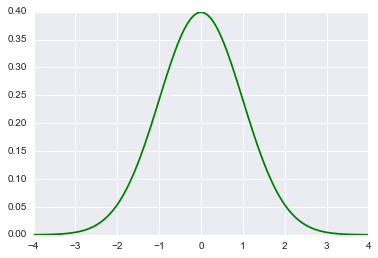
\includegraphics[scale=0.55]{normal}
\end{figure}

Como la densidad solo depende de \(\mu\) y \(\sigma^2\), conociendo estos dos valores se define por completo su función de distribución. Más aún, estos valores coinciden con la media y la varianza, por lo que la distribución normal es definida completamente con sus dos primeros momentos:
\begin{align*}
	\mean(X)		&= \mu,\\
	\variance(X)	&= \sigma^2.
\end{align*}
Para ayudar a entender por qué esta distribución es tan importante, se mencionan a continuación algunas de las propiedades que la distribución normal cumple.

\begin{proposition}
	Si \(X\sim \calN (\mu, \sigma^2)\) entonces se tiene que:
	\begin{itemize}
		\item Su función de densidad es simétrica respecto a su media, es decir, \(f(\mu + x; \mu, \sigma) = f(\mu - x; \mu, \sigma)\).
		\item La moda, la media y la mediana de \(X\) coinciden y todas son iguales a \(\mu\).
		\item La densidad se concentra en torno a \(\mu\) vía la regla empírica «\(68\), \(95\), \(99.7\)»:
		\begin{align*}
			\prob(\vert X - \mu \vert \leq \sigma)		& \approx 0.6826,\\
			\prob(\vert X - \mu \vert \leq 2 \sigma)	& \approx 0.9544,\\
			\prob(\vert X - \mu \vert \leq 3 \sigma)	& \approx 0.9974.
		\end{align*}
		\item La transformación lineal de una variable normal sigue siendo una variable normal escalada de la forma \(aX + b \sim \calN(a \mu + b, a^2\sigma^2)\).
		\item La suma de dos variables normales independientes sigue siendo una variable normal. Si \(X\sim \calN (\mu_X, \sigma_X^2)\), \(Y\sim \calN (\mu_Y, \sigma_Y^2)\) y \(X \perp Y\), entonces \(X + Y \sim \calN (\mu_X + \mu_Y, \sigma_X^2 + \sigma_Y^2)\).
	\end{itemize}
\end{proposition}

La distribución normal no solo cumple estas propiedades simples, sino que está presente en algunos resultados de diferentes áreas, tales como estadística, procesamiento de señales, y ecuaciones diferenciales, por nombrar algunas. A continuación se listan tres resultados de la matemática donde el objeto principal es la distribución normal. Se comienza primero con un importante resultado sobre el promedio de variables aleatorias.

\begin{theorem}[Teorema del Límite Central] Sea \((X_n)_{n \in \naturals}\) una sucesión de variables aleatorias, independientes e idénticamente distribuidas (i.i.d.) de media \(\mu\) y varianza \(\sigma^2\). Sea
	\[\bar{X}_{n} = \frac{X_1 + \dotsb + X_n}{n}.\]
	Entonces se tiene el siguiente resultado con respecto al límite:
	\begin{equation*}
		\lim_{n \to \infty} \sqrt{n} \left(\frac{\bar{X}_n - \mu }{\sigma}\right) \sim \calN (0, 1).
	\end{equation*}
\end{theorem}

En términos informales, se puede ver que si \(n\) es lo suficientemente grande, entonces el promedio \(\bar{X}_n\) converge a una distribución normal \(\calN (\mu, \frac{\sigma^{2}}{n})\). Cabe destacar que este resultado no tiene ningún supuesto sobre la distribución de las variables aleatorias \(X_i\).

La función de densidad de la distribución normal cumple otra propiedad interesante en el área de procesamiento de señales. Es necesario definir una famosa transformación lineal de funciones, la llamada transformada de Fourier.
\begin{definition} La Transformada de Fourier \(\calF : L^2(\reals) \to L^2(\complex)\) es una aplicación lineal continua entre espacios de funciones integrables de valores reales a valores complejos, que transforma una función \(f(t)\) a otra \(\hat{f}(w)\) de la siguiente forma:
	\begin{equation*}
		\calF \left[ f(t) \right] = \hat{f}(w) = \frac{1}{\sqrt{2\pi}} \int_{-\infty}^\infty f(t) e^{-iwt} \dd{t}.
	\end{equation*}
\end{definition}

En procesamiento de señales, la transformada de Fourier suele considerarse como la descomposición de una señal en componentes de frecuencias diferentes, es decir, \(\hat{f}(w)\) corresponde al espectro de frecuencias de la señal \(f(t)\). Una propiedad interesante que cumple la función de densidad de una gaussiana estándar es ser punto fijo de la transformada de Fourier.

\begin{proposition}
	La transformada de Fourier de una función gaussiana de media 0 y varianza 1 también es una función gaussiana de media 0 y varianza 1, es decir,
	\begin{align*}
		f(t)		&= e^{-\frac{t^{2}}{2}}, \\
		\hat{f}(w)	&= e^{-\frac{w^{2}}{2}}.
	\end{align*}
\end{proposition}

Finalmente, en el área de ecuaciones diferenciales parciales la función de densidad de una gaussiana también cumple con un rol importante, ya que es la solución de la ecuación del calor homogénea.

\begin{proposition}
	Considere la siguiente ecuación en derivadas parciales con condición inicial de parámetro \(\frac{\sigma^{2}}{2}\):
	\begin{align*}
		\pdv{f(x, t)}{t} - \frac{\sigma^2}{2}\pdv[2]{f(x, t)}{x}	&= 0 \text{ para } (x, t) \in \reals \times (0, \infty), \\
		f(x, 0)														&= \delta(x) \text{ para } x \in \reals.
	\end{align*}
	Esta ecuación tiene como solución la función gaussiana:
	\[f(x, t) = \frac{1}{\sigma \sqrt{2\pi t}} e^{-\frac{x^2}{2\sigma^2 t}}.\]
\end{proposition}

\section{Procesos Estocásticos y Campos Aleatorios}
Ahora que una variable aleatoria está definida, se puede introducir el concepto de proceso estocástico, que corresponde a una sucesión de variables aleatorias que cumplen alguna ley de probabilidad conjunta.

\begin{definition}
	Dado un espacio de probabilidades \((\Omega, \calB, \prob)\), un proceso estocástico \(\{X_t\}_{t \in \calT}\) es una colección de vectores aleatorios \(X_t : \Omega \to \reals^{n}\) de dimensión \(n\) e indexadas por un conjunto de índices (o parámetros) \(\calT\).
\end{definition}

\begin{figure}[h]
	\centering
	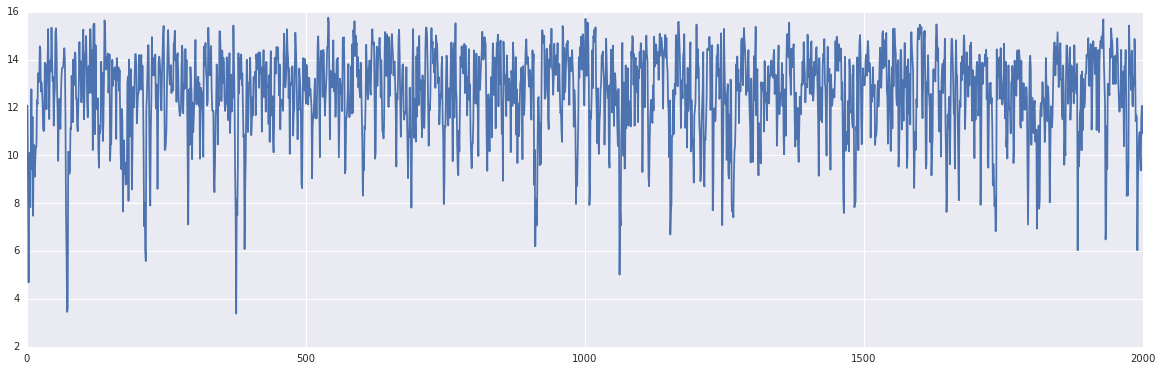
\includegraphics[scale=0.4]{stochasticprocesses}
\end{figure}

Por simplicidad de notación vamos a denotar \(\{X_t\}_{t \in \calT}\) al proceso estocástico, y a continuación mostraremos una clasificación que se puede encontrar en la literatura. El conjunto \(\calT\) es conocido como espacio de parámetros\footnote{No confundir con el concepto de parámetros de una distribución o función paramétrica.} (\emph{parameter space} en inglés), y si es un intervalo de \(\reals\) (los reales no negativos normalmente) se dice que el proceso \(\{X_t\}_{t \in \calT}\) es a tiempo continuo. Si \(\calT\) es un conjunto numerable (los números naturales normalmente), entonces se dice que el proceso \(\{X_t\}_{t \in \calT}\) es a tiempo discreto. En el caso de que \(\calT\) sea un espacio topológico de mayor dimensión (\(\reals^{d}\) por ejemplo), se dirá que \(\{X_t\}_{t \in \calT}\) es un campo aleatorio (o \emph{random field} en inglés).

La imagen de \(X_t\) es conocida como espacio de estados (o \emph{state space} en inglés). En el caso en que los estados son discretos, si el tiempo es discreto también se dice que el proceso es una cadena, y si el tiempo es continuo entonces se dice que es un proceso puntual. En cambio, si los estados y el tiempo son continuos se dice que el proceso es continuo, y si sólo el tiempo es discreto entonces se dice que el proceso es una sucesión discreta de variables aleatorias, donde una realización parcial del proceso se llama serie temporal.

\subsection{Teorema de Consistencia de Kolmogorov}

Así como existe el concepto de función de distribución para variables aleatorias, este se puede extender al caso multidimensional de forma directa. Sea \(X_1, \dotsc, X_n\) un conjunto de variables aleatorias. La función de distribución conjunta del vector aleatorio \((X_1, \dotsc, X_n)\) es de la forma
\[F(c_1, \dotsc, c_n) = \prob(\{\omega : X_i(\omega) \leq c_{i} \text{ para todo } i\}).\]

Mientras que el enfoque de teoría de la medida parte con un espacio de probabilidades para definir a los procesos estocásticos, el enfoque de aprendizaje de máquinas parte desde una colección de leyes finito-dimensionales, que mediante el Teorema de Consistencia de Kolmogorov es posible construir modelos predictivos.

\begin{definition}
	La familia de distribuciones finito-dimensionales del proceso estocástico \(\{X_t\}_{t \in \calT}\) es una colección de funciones \(\calF = \{F_{t_1, \dotsc, t_n} : t_1, \dotsc, t_n \in \calT, n \in \naturals\}\) que, dada una colección finita cualquiera de puntos \(t_1, \dotsc, t_n\in \calT\), la distribución conjunta del vector aleatorio \((X_{t_1}, \dotsc, X_{t_n})\) está dada por \(F_{t_1, \dotsc, t_n} (c_{1}, \dotsc, c_n)\).
\end{definition}

El conjunto \(\calF\) de familia de distribuciones finito-dimensionales satisface las bien conocidas condiciones de consistencia de Kolmogorov:
\begin{enumerate}
	\item \textbf{Permutación}: para cualquier \(n\)-permutación \(\pi\), conjunto de índices \(t_1, \dotsc,t_{n} \in \calT\) y valores \(x_1, \dotsc,x_n \in \calX\) se tiene que
	\[F_{t_{\pi(1)}, \dotsc, t_{\pi(n)}} \left(x_{\pi(1)}, \dotsc, x_{\pi(n)}\right) = F_{t_1, \dotsc, t_n} \left(x_1, \dotsc, x_n\right).\]
	\item \textbf{Marginalización}: para cualquier conjunto de índices \(t_1, \dotsc, t_{n+m} \in \calT\) y todo conjunto de valores \(x_1, \dotsc, x_n \in \calX\) se tiene que
	\[F_{t_1, \dotsc, t_{n+m}} (x_1, \dotsc, x_n, +\infty, \dotsc, +\infty) = F_{t_1, \dotsc, t_n} (x_1, \dotsc, x_n).\]
\end{enumerate}

Si una familia de distribuciones finito-dimensional \(\calF\) satisface las condiciones de consistencia, entonces el \emph{Teorema de Consistencia de Kolmogorov} \cite{tao2011introduction} nos permite construir un proceso estocástico \(\hat{f} = \{\hat{f}_t\}_{t \in \calT}\) tal que su familia de distribuciones finito-dimensionales \(\hat{\calF}\) coincide con \(\calF\). La implicancia de este resultado repercute en el aprendizaje de máquinas de modo que, al tener una regla para construir un conjunto de distribuciones finito-dimensionales de forma consistente, podemos calcular probabilidades posteriores de cualquier vector aleatorio \(X\) dados los datos \(E\).

Como la ley de un proceso estocástico está completamente determinada por la asociada familia de leyes finito-dimensionales (l.f.d. de ahora en adelante) \cite{ross1996stochastic}, por abuso de notación nos referiremos a su ley como \(\calF\). Ahora podemos caracterizar al proceso \(\{X_t\}_{t \in \calT}\) según las propiedades que cumple su familia de leyes finito-dimensionales. Así como una variable aleatoria tiene media y varianza, un proceso estocástico tiene una función de media y una función de covarianza, definidas a continuación.

\begin{definition}
	Dado un un proceso estocástico \(\{X_t\}_{t \in \calT}\), sus funciones de media \(\mu\) (también denotada como \(m\)) y de covarianza \(k\) se definen como
	\begin{align*}
		\mu(t)	&= \mean(X_t), \\
		k(t, s)	&= \cov(x_t, x_s) = \mean\left[(x_t - \mu(t)) (x_s - \mu(s))\right].
	\end{align*}
\end{definition}

Cabe destacar que \(k(t, t) = \cov(x_t, x_t) = \variance(x_t)\). A continuación definiremos dos propiedades interesantes sobre las l.f.d. y las funciones de media y covarianza.

\begin{definition}
	Un proceso estocástico \(\{X_t\}_{t \in \calT}\) se dice estacionario débil si \(\mu(t) = \mu\), \(k(t, t) = \sigma^2\) y para cualquier índice \(j\), \(k(t, t + j) = k(s, s + j) = \sigma_j\).
\end{definition}

\begin{definition}
	Un proceso estocástico \(\{X_t\}_{t \in \calT}\) se dice estacionario fuerte si sus l.f.d. son invariantes a la traslación temporal, es decir, para todo \(\tau \in \calT\) se tiene que \(F_{t_1, \dotsc, t_N} = F_{t_1 + \tau, \dotsc, t_N + \tau}\).
\end{definition}

El siguiente resultado caracteriza la función de covarianza en el caso que el proceso sea estacionario fuerte, en particular estacionario débil.
\begin{proposition}
	Si \(\{X_t\}_{t \in \calT}\) es estacionario fuerte, entonces es estacionario débil. En ese caso, su función de covarianza se puede escribir en función de la distancia del tiempo, es decir \(k(t, s) = k(t - s, 0) = k_\rho( t - s)\).
\end{proposition}

En general, un proceso estacionario débil no es necesariamente estacionario fuerte. Sin embargo, la clase de procesos conocidos como procesos gaussianos cumple con la propiedad de que las nociones de estacionalidad débil y fuerte coinciden. Esta es una de mucha propiedades que poseen, que son de gran utilidad para la modelación de procesos estocásticos.

\subsection{Normal Multivariada}
Como vimos anteriormente, la función gaussiana tiene una naturaleza tan especial que la hace un objeto de estudio aplicado a diferentes áreas de las matemáticas y de las ciencias en general. Veamos a continuación como se generaliza esta función a múltiples dimensiones.

\begin{figure}[h]
	\centering
	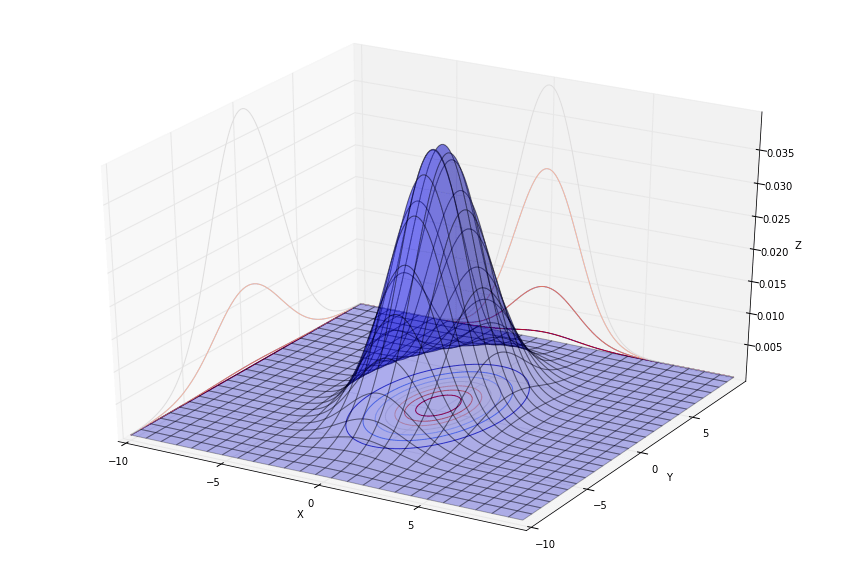
\includegraphics[scale=0.5]{gaussian2d}
\end{figure}

\begin{definition}
	Sea \(\bfx = (X_1, \dotsc, X_n)\) un vector aleatorio de dimensión \(n\). Se dice que \(\bfx\) es conjuntamente gaussiano de vector de media \(\mu_\bfx \in \reals^n\) y matriz de covarianza \(\Sigma_\bfx \in \reals^{n \times n}\) definida positiva, si su función de densidad conjunta \(f_{1, \dotsc, n}\) es de la forma
	\begin{equation*}
		f_{1, \dotsc, n}(\bfx) = \frac{1}{(2 \pi)^{\frac{n}{2}} \left\vert \Sigma_\bfx \right\vert^{\frac{1}{2}}} e^{-\frac{1}{2} (\bfx - \mu_\bfx)^\top \Sigma_\bfx^{-1} (\bfx - \mu_\bfx)}.
	\end{equation*}
\end{definition}
Por abuso de notación vamos a identificar la densidad conjunta con la distribución, es decir \(f_{1, \dotsc, n}(\bfx) = \calN_{n} (\mu_{\bfx}, \Sigma_{\bfx,\bfx})\). La siguiente proposición entrega una caracterización diferente de una normal multivariada:
\begin{proposition}
	El vector aleatorio \(\bfx = (X_1, \dotsc, X_n)\) de media \(\mu\) y matriz de covarianza \(\Sigma\) es conjuntamente gaussiana si satisface las siguientes condiciones equivalentes:
	\begin{itemize}
		\item Toda combinación lineal \(Y = a_1 X_1 + \dotsb + a_n X_n\) está normalmente distribuida.
		\item Existe una matriz \(L\) de tamaño \(n \times m\) tal que \(\Sigma = LL^\top\) y \(\bfz = (Z_1, \dotsc, Z_m)\) un vector aleatorio de \(m\) variables aleatorias normales independientes de media nula y varianza unitaria de modo que \(\bfx = L \bfz + \mu\).
	\end{itemize}
\end{proposition}
\subsection{Consistencia}

Como veremos, la distribución gaussiana satisface propiedades útiles para nuestros propósitos, es decir, las condiciones de consistencia de Kolmogorov. Sean \(\bfx : \Omega \to \calX^n, \bfxo : \Omega \to \calX^{\no}\) vectores aleatorios indexados por los tiempos disjuntos \(\bft\) y \(\bfto\) respectivamente. Si ambos vectores son conjuntamente distribuidos gaussianos entonces tenemos que
\begin{equation*}
	f_{\bft, \bfto} \left(\bfx, \bfxo\right) = \calN_{n + \no} \left( \begin{bmatrix} \mu_{\bfx} \\ \mu_{\bfxo} \end{bmatrix},
	\begin{bmatrix}
		\Sigma_{\bfx} & \Sigma_{\bfx \bfxo} \\
		\Sigma_{\bfxo \bfx} & \Sigma_{\bfxo}
	\end{bmatrix} \right).
\end{equation*}

La condición de marginalización se satisface debido a que
\[ \int_{\calX^n} f_{\bft, \bfto} (\bfx, \bfxo) \dd{\bfx} = \calN_{\no} (\mu_{\bfxo}, \Sigma_{\bfxo,\bfxo}) = f_{\bfto} (\bfxo),\]
y la condición de permutación se satisface ya que dada una \(n\)-permutación \(\pi\), existe una matriz de permutación \(P\) tal que \(P^{-1} = P^\top\) y se satisface que
\[f_{\pi(\bft)}(\pi(\bfx)) = \frac{1}{\left(2\pi\right)^{\frac{n}{2}} \left\vert P \Sigma P^\top \right\vert^{\frac{1}{2}}} e^{-\frac{1}{2} (\bfx - \mu)^\top P^\top (P\Sigma P^{\top})^{-1} P (\bfx - \mu)} = f_{\bft}(\bfx).
\]

\subsection{Procesos Gausianos}

Debido a su consistencia bajo marginalización y permutación, podemos extender la distribución gaussiana al caso infinito-dimensional gracias al Teorema de Consistencia de Kolmogorov. A esta construcción se le conoce como proceso gaussiano (o GP) \cite{rasmussen06}, que se puede interpretar como una distribución de probabilidades a priori sobre funciones que definen modelos de regresión no lineales y no paramétricos.

\begin{definition}
	Un proceso estocástico \(\{X_t\}_{t \in \calT}\) se dice un proceso gaussiano si sus distribuciones finito dimensionales son distribuciones gaussianas.
\end{definition}

Una de las principales ventajas es que un proceso gaussiano \(\{X_t\}_{t \in \calT}\) está completamente definido con su función de media \(\mu(t)\) y de covarianza \(k(t, s)\), por lo que denotamos que \(X_t \sim \GP(\mu(t), k(t, s))\). Por esta razón, la propiedad de estacionalidad fuerte coincide con la propiedad de estacionalidad débil.

\begin{proposition}
	Dado un proceso gaussiano \(\{X_t\}_{t \in \calT}\), todas sus propiedades de distribución son determinadas por sus funciones de media \(\mu(t)\) y de covarianza \(k(t, s)\). En particular, el proceso gaussiano será estacionario fuerte si su función de media es constante y la función de covarianza es en función de la diferencia temporal, es decir \(\mu(t) = \mu\) y \(k(t, s) = k_\rho(t - s)\).
\end{proposition}

\subsection{Proceso Browniano}
Uno de los procesos estocásticos más utilizado en probabilidades es el proceso de Wiener, más conocido como movimiento browniano (\emph{Brownian motion} en inglés), el cual es utilizado fuertemente para resolver ecuaciones diferenciales estocásticas y definir objetos matemáticos tales como la integral estocástica. Este proceso es un caso particular de proceso gaussiano, en donde la función de media es nula y su función de covarianza está dada por \(k(t, s) = \min\{t, s\}\).

\subsection{Machine Learning}

Los parámetros de \(\mu(t)\) y \(k(t, s)\) son llamados los \emph{hiperparámetros} del GP. En la Figura \ref{fig:gp_sunspots_example} se muestra un gráfico de un ejemplo de GP con una función de covarianza muy utilizada, llamada \emph{squared exponential} (SE), dada por
\begin{align*}
	k_{\mathrm{SE}}(t, s) = \sigma^2 \exp\left(-\frac{(t-s)^2}{l^2}\right),
\end{align*}
donde \(\sigma^2 > 0\), y \(l > 0\) son los \emph{hiperparámetros} del GP.

Dada un vector de puntos \(\bft \in \calT^n\), denotemos la evaluación de la función de media \(\mu\) en \(\bft\) de tal forma que el vector \(\mu(\bft)_i = \mu(t_i)\) para \(i \in \{1,...,n\}\). De forma análoga, dados dos vectores de puntos \(\bft \in \calT^n\) y \(\bfto \in \calT^{\no}\), denotemos la evaluación de la función de covarianza \(k\) en \(\bft,\bfto\) de modo que la matriz \([k(\bft,\bfto)]_{i,j} = k(t_i,\bar{t}_j)\) para \(i \in \{1,...,n\}\) y \(j \in \{1,...,\no\}\).

Mientras no haya ambigüedad en la selección de los puntos \(\bft\), denotaremos \(X_\bft\) como \(\bfx\), \(\mu(\bft)\) como \(\mu_{\bfx}\) y \(k(\bft,\bft)\) como \(\Sigma_{\bfx}\). Para una segunda colección de puntos \(\bfto\) la notación es análoga: la evaluación del proceso es \(X_{\bfto} = \bfxo\), la media es \(\mu(\bfto) = \mu_{\bfxo}\), la covarianza \(k(\bfto,\bfto) = \Sigma_{\bfxo}\) y la covarianza cruzada entre \(\bfx\) y \(\bfxo\) se denota \(k(\bft, \bfto) = \Sigma_{\bfx \bfxo}\).

Para hacer inferencia en nuevos \emph{inputs} \(\bfto\) basta con calcular la distribución posterior de \(\bfxo\) dada las observaciones \(\bfx\), la cual también es gaussiana y sigue la distribución
\[f_{\bfto \mid \bft}(\bfxo \mid \bfx) = \calN(\bfxo \mid \mu_{\bfxo \mid \bfx}, \Sigma_{\bfxo \mid \bfx}),\]
donde
\begin{align*}
	\mu_{\bfxo \mid \bfx}	&= \mu_{\bfxo} + \Sigma_{\bfxo\bfx} \Sigma_{\bfx\bfx}^{-1} (\bfx - \mu_{\bfx}),\\
	\Sigma_{\bfxo \mid \bfx}	&= \Sigma_{\bfxo \bfxo} - \Sigma_{\bfxo \bfx} \Sigma_{\bfx \bfx}^{-1} \Sigma_{\bfx \bfxo},
\end{align*}
se conocen como la media y la covarianza condicional respectivamente; esos estadísticos permiten calcular estimaciones puntuales, intervalos de confianza y muestrear funciones directamente. En la Figura \ref{fig:gp_sunspots_example} mostramos la posterior de un GP con kernel SE sin entrenar y con entrenar, dado un conjunto de observaciones de datos de actividad solar.

\begin{figure}[h]
	\centering
	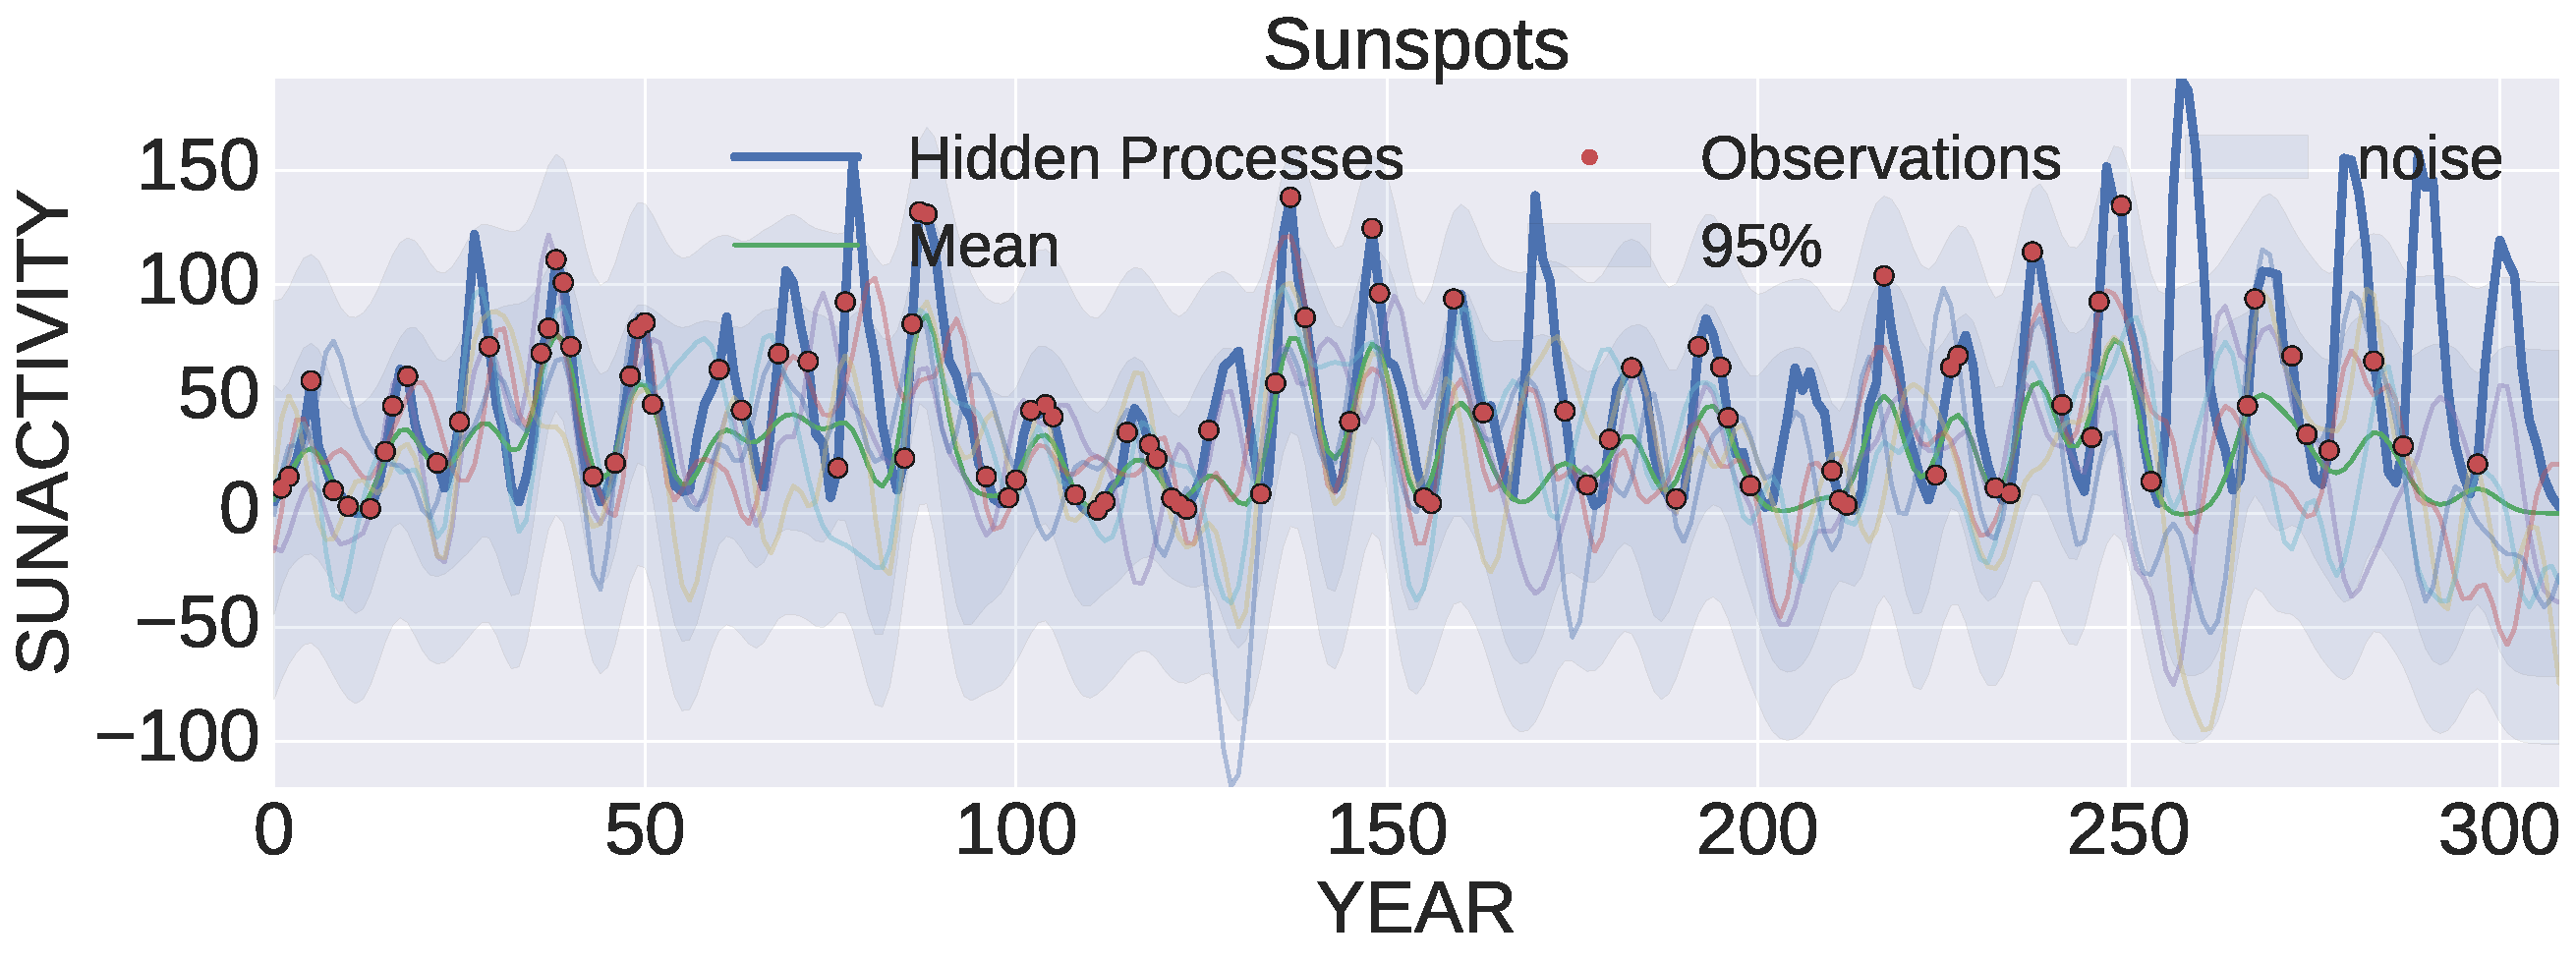
\includegraphics[width=0.49\textwidth]{gp_sunspots1}
	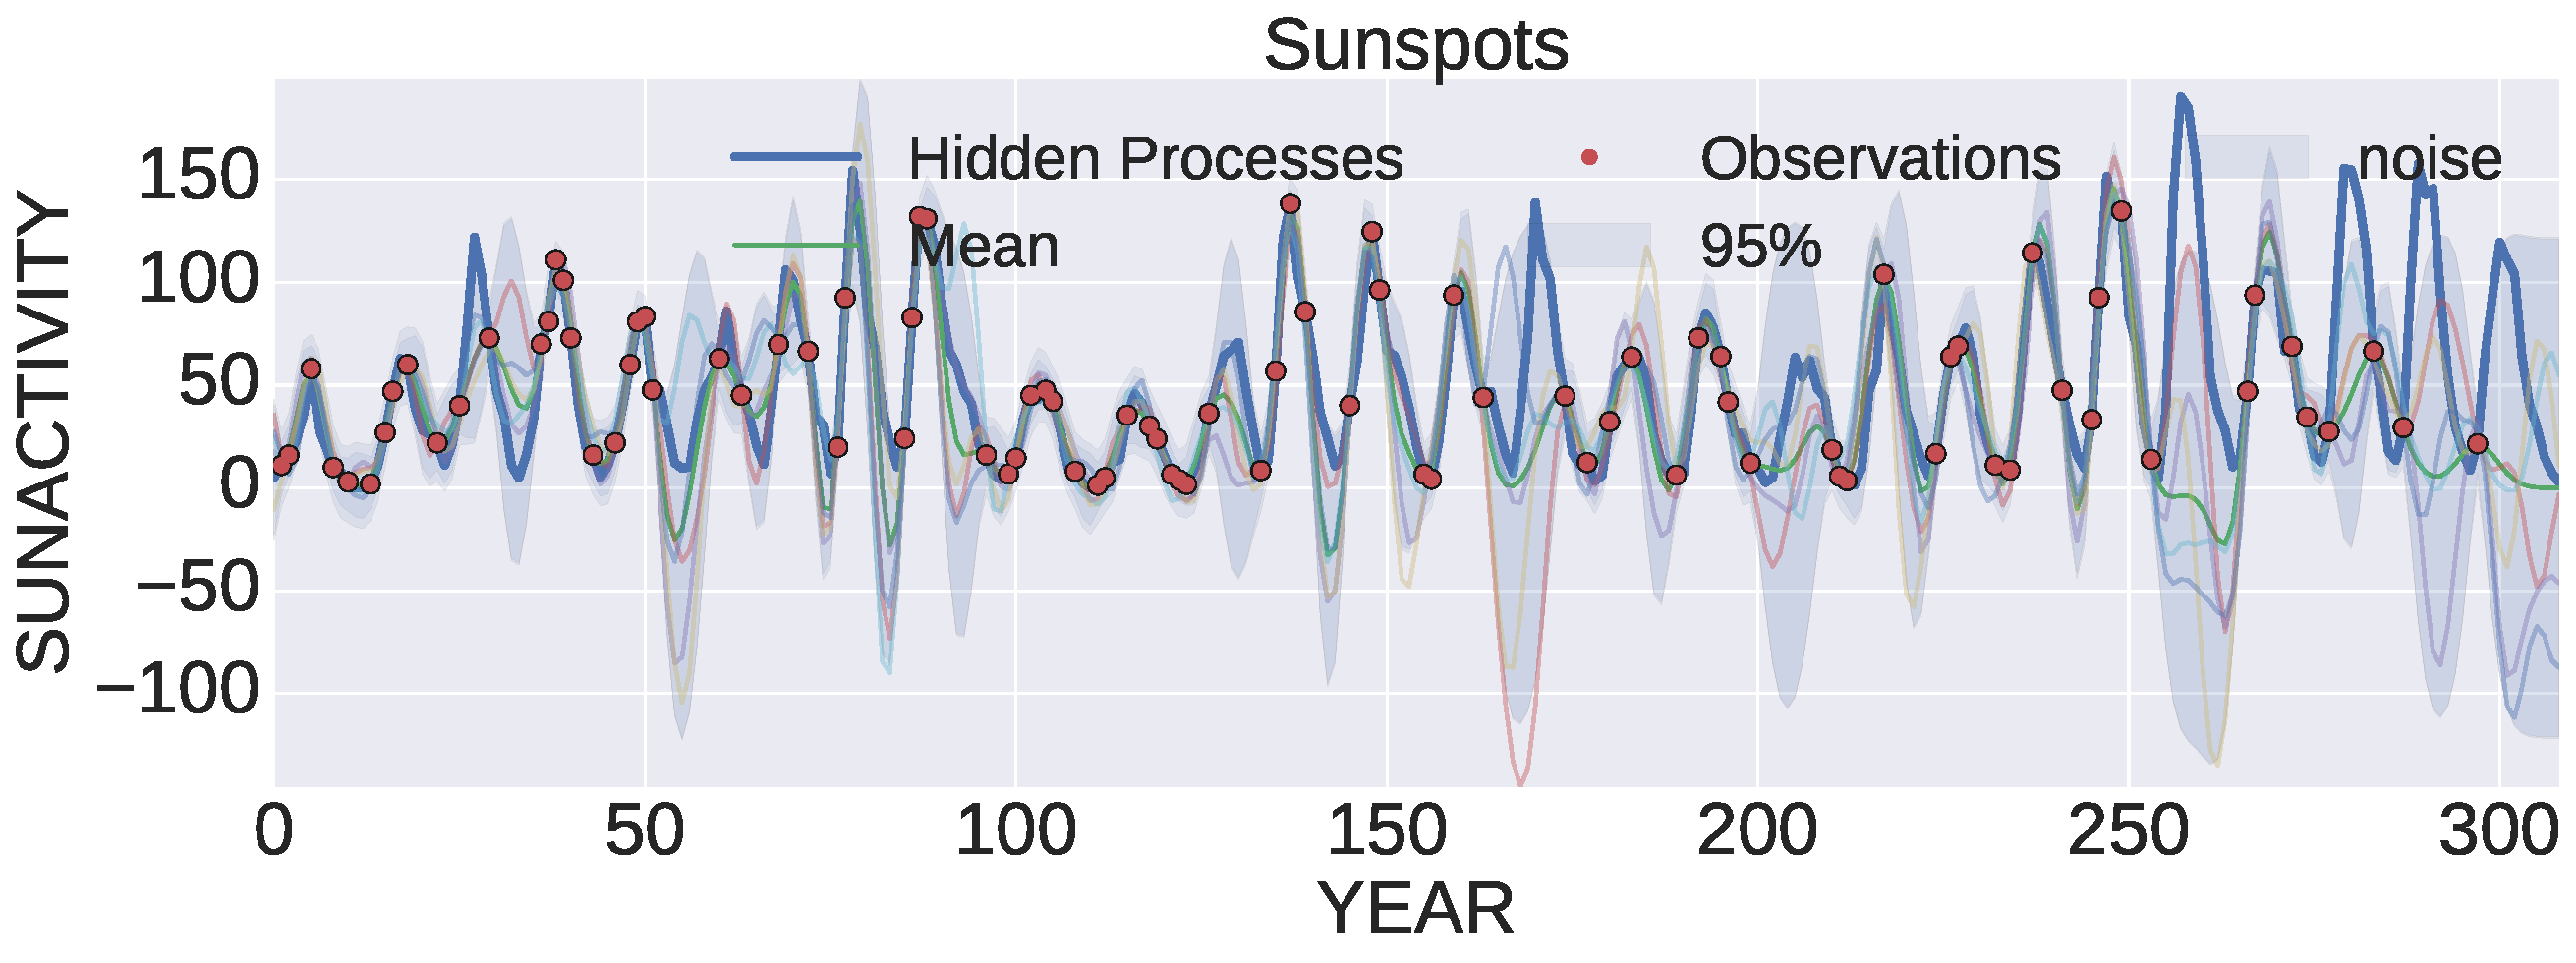
\includegraphics[width=0.49\textwidth]{gp_sunspots2}
	\caption{La distribución posterior de un GP. Izquierda: GP no entrenado. Derecha: GP entrenado.}
	\label{fig:gp_sunspots_example}
\end{figure}

El kernel usualmente se escoge heurísticamente basado en la experiencia y el conocimiento a priori del fenómeno a modelar. En la Figura \ref{fig:gp_kernels} consideramos la inferencia sobre las mismas cuatro observaciones, pero tres diferentes kernels:
\begin{itemize}
	\item Ornstein-Uhlenbeck: \(k_{\mathrm{OU}}(t, s) = \sigma^2 \exp\left(-\frac{\lvert t-s \rvert}{2l^2}\right)\),
	\item \emph{Rational Quadratic}: \(k_{\mathrm{RQ}}(t, s) = \sigma^2 \left(1 + \frac{\lvert t - s \rvert^2}{2\alpha l^2}\right)^{-\alpha}\),
	\item \emph{Locally Periodic}: \(k_{\mathrm{per}}(t, s) = \sigma^2 \exp\left(-\frac{\lvert t - s \rvert^2}{2l^2}\right) \exp\left(-\frac{2\sen^2 (\pi \lvert t - s \rvert/p)}{l^2}\right)\).
\end{itemize}
\begin{figure}[h]
	\centering
	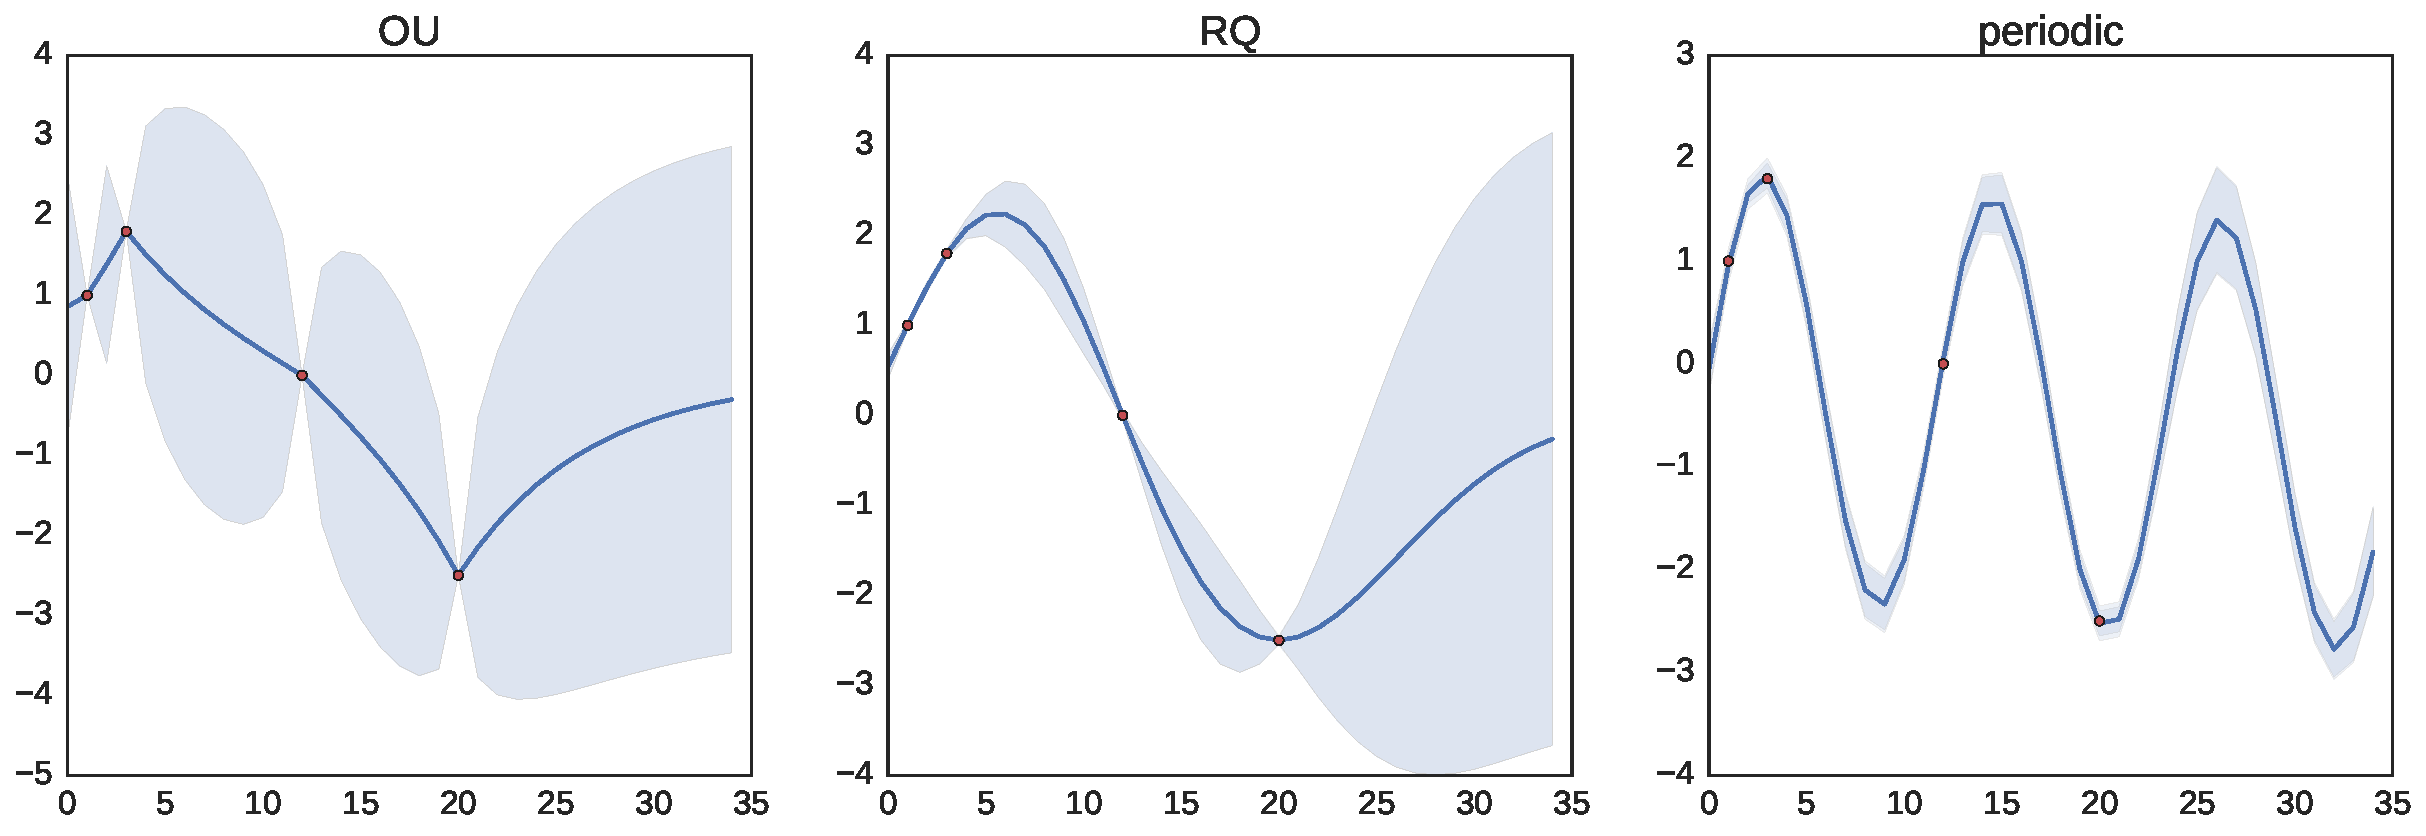
\includegraphics[width=0.8\textwidth,height=0.22\textwidth]{kernels2}
	\caption{La distribución posterior de GP con diferentes funciones de kernels, pero las mismas observaciones. Izquierda: Ornstein-Uhlenbeck, centro: \emph{Rational Quadratic}, derecha: \emph{Locally Periodic}.}
	\label{fig:gp_kernels}
\end{figure}

Dadas las observaciones \((\bft,\bfx)\), entrenar es equivalente a encontrar un kernel \(k\) y una función de media \(m\), usualmente parametrizadas por un vector de hiperparámetros finito \(\theta = (\theta_k, \theta_m) \in \reals^p\), el cual se encuentra al minimizar la log-verosimilitud negativa (NLL por sus siglas en inglés), dada por
\[-\log p_{\bft}(\bfx \mid \theta) = \frac{n}{2} \log(2\pi) + \frac{1}{2} (\bfx - \mu_{\bfx} )^\top \Sigma_{\bfx \bfx}^{-1} (\bfx - \mu_{\bfx}) + \frac{1}{2} \log \lvert \Sigma_{\bfx \bfx} \rvert,\]
donde \(\mu_\bfx\) y \(\Sigma_{\bfx \bfx}\) son la media y la covarianza de \(\bfx\) dados los hiperparámetros \(\theta = (\theta_k, \theta_m)\). Los métodos más utilizados son los basados en el gradiente de cuasi-Newton BFGS y el método libre de derivadas de Powell. En la Figura \ref{fig:gp_sunspots_example} mostramos un GP con kernel SE, dadas observaciones de datos de actividad solar, donde el gráfico de la izquierda tiene hiperparámetros por defecto, mientras que el gráfico de la derecha tiene hiperparámetros entrenados. En el caso entrenado la media pasa cerca de la señal real y los intervalos de confianza son pequeños, por lo que la predicción tiene menos incertidumbre.

\comment{Parrafo: consolidar y resumir las ideas explicadas en el capitulo, mencionar que temas se profundizarán en otras partes del libro.}

En el capítulo de procesos gaussianos vamos a volver a revisar todo esto pero con mayor detalles, pero esta sección es una rápida introducción de como utilizar este objeto matemático para hacer predicciones.
	%!TEX root = main.tex

\chapter{Paradigma Bayesiano}

\begin{chapquote}{Dennis Lindley}
	``Dentro de cada no bayesiano, hay un bayesiano que lucha por salir.''
\end{chapquote}

\comment{extender un poco y suavizar más la entrada a temas duros, incluir un mini resumen del capitulo}
Lo que inicialmente nos motivó a estudiar el enfoque bayesiano son los llamados modelos no paramétricos: aquellos modelos que, a pesar de su nombre, tienen infinitos (o un número ilimitado de) parámetros que aumenta a medida de que observamos más datos. Algunos ejemplos comunes de modelos no paramétricos son los histogramas y las funciones de \emph{spline}, pero los basados en estadísticas bayesianas tienen una matemática más elegante y formal, coincidiendo en muchos aspectos con los procesos estocásticos. Un ejemplo de esto es el llamado proceso de Dirichlet, una distribución sobre distribuciones discretas, por lo que es muy útil en problemas de agrupamiento. Otro ejemplo distinguido con los procesos gaussianos, ya que se interpretan como distribuciones sobre espacios de funciones, muy útil en problemas de regresión. Este será el modelo de estudio en gran parte del libro.

\section{Modelos Bayesianos}

Consideremos las observaciones \(\calD = \{x_1, \dotsc, x_n\}\) de un espacio de datos \( \calX\) (por ejemplo \(\calX \subset \reals^q\)) y un conjunto de posibles modelos o medidas de probabilidades \(\calM \subseteq \calP(\calX)\), donde \(\calP(\calX)\) es el conjunto de medidas de probabilidad en \(\calX\). Por ejemplo, sea \(\calX=\{0,1\}\) tal que \[\calM = \{m_{\alpha} \in \calP(\calX) \mid m_\alpha(\{0\})=\alpha, m_\alpha(\{1\})=1-\alpha\text{, para } \alpha \in [0,1] \}\] es el espacio de distribuciones Bernoulli.


Entrenar un modelo, también conocido como selección de modelos, consiste en escoger un modelo \(m \in \calM\) que \emph{mejor} explique los datos \(\calD\) generados por \(m\), bajo algún criterio \cite{chipman2001practical}. Nosotros adoptamos el paradigma bayesiano, el cual provee de un marco probabilista para lidiar con la incertidumbre del modelo, en términos de una \emph{distribución a priori} \(\Pi\) sobre el espacio de modelos \(\calM\); referimos al lector a \cite{ghosal2017fundamentals, murphybook2012} y sus referencias para un trasfondo matemático de estadística bayesiana y métodos. Un desafío crítico en la perspectiva bayesiana es calcular la ley predictiva en \(\calX\), usualmente llamada la \emph{posterior predictiva} \cite{gelman2013bayesian}, desde la distribución posterior en \(\calM\).

Consideremos una medida de probabilidad \emph{a priori} \(\Pi\) sobre el espacio de modelos \(\calM\), es decir \(\Pi \in \calP(\calM)\). Siguiendo nuestro ejemplo consideremos \(\Pi\) sobre \(\calM\) de modo que \(\Pi(\{m_\alpha \mid \alpha \in A\}) = \lambda(A)\) para \(A \subseteq [0,1]\), donde \(\lambda\) denota la medida de Lebesgue. 


En virtud del Teorema de Bayes, la medida \emph{posterior} \(\Pi(\dd{m} \mid x_1, \dotsc, x_n)\) de modelos dados los datos \(\calD\), la cual se denota por simplicidad \(\Pi_n(\dd{m})\), está dada por
\begin{equation}\label{eq def Pi n}
	\Pi_n(\dd{m}) \coloneqq \frac{\Pi \left(x_1, \dotsc, x_n \mid m\right) \Pi \left(\dd{m}\right)}{\Pi \left(x_1, \dotsc, x_n\right)},
\end{equation}
donde \(\Pi(x_1, \dotsc, x_n) = \int_{\calM} \Pi(x_1, \dotsc, x_n \mid m) \Pi(\dd{m})\) es la verosimilitud marginal o \emph{evidencia} (constante con respecto a \(m\)), mientras que \(\calL_n(m) = \Pi  \left(x_1, \dotsc, x_n \mid m\right)\) es la función de \emph{verosimilitud}. Para nuestro ejemplo, denotando \(\bar{x} = \frac{1}{n}\sum_{i=1}^n x_i\), la función de \emph{verosimilitud} está dada por \(\calL_n(m_\alpha) = \alpha^{n \bar{x}} (1-\alpha)^{n (1-\bar{x})}.\)

\comment{parrafo: explicar intuición de lo recien explicado, puede ir antes o despues de la matematica dura}



\section{Enfoque Paramétrico}

En general supondremos que \(\calM \subseteq \calP_{\mathrm{ac}}(\calX)\), donde \(\calP_{\mathrm{ac}}(\calX)\) es el subconjunto de medidas absolutamente continuas con respecto a una misma medida \(\sigma\)-finita \(\lambda\) en \(\calX\) (por ejemplo la medida de Lebesgue). Como convención, usaremos la misma notación para un elemento \(m(\dd{x}) \in \calM\) y su densidad \(m(x)\) con respecto a \(\lambda\). \comment{luego de la explicación dura, explicarlo en palabras}

Se dice que \(\calM\) está finitamente parametrizado si hay un número \(k \in \naturals\), un conjunto \(\Theta \subseteq \reals^k\) llamado el espacio de parámetros, y una función (medible) \(\calI : \Theta \to \calP_{\mathrm{ac}}(\calX)\), llamado el mapeo de parametrización, tales que \(\calM = \calI(\Theta)\). En dicho caso denotamos \(m_\theta \coloneqq \calI(\theta)\). Siguiendo nuestro ejemplo, donde \(m_\alpha({0}) = \alpha\) y \(m_\alpha({1}) = 1-\alpha\), consideremos el espacio de parámetros \(\Theta = [0,1]\) y definimos dos mapas de parametrización: \(\calI_0(\theta) = m_\theta\) y \(\calI_1(\theta) = m_{\theta^{1/2}}\).

Dado \(p \in \calP(\Theta)\) una distribución a priori sobre el espacio de parámetros \(\Theta\), la medida \emph{push-forward}\footnote{«Que empuja hacia adelante» en español pero usaremos el anglicismo por comodidad.} a través del mapa \(\calI\) es la medida de probabilidad \(\Pi=\calI(p)\) sobre el espacio de modelos parametrizados \(\calM = \calI(\Theta)\), dado por \(\Pi(A)= p(\calI^{-1}(A))\) para \(A \in \mathcal{B}(\calM)\). Análogamente, como definimos el prior \(\Pi(\{m_\alpha \mid \alpha \in A\}) = \lambda(A)\), el prior inducido sobre \(\Theta\) corresponde a \(p(A) = \Pi(\calI(A)) \) para \(A \in \mathcal{B}(\Theta)\). Bajo la parametrización natural \(\calI_0\), el prior sobre \(\Theta\) es \(p_0(\theta) = \mathbf{1}_{\{\theta \in [0,1]\}}(\theta)\) y bajo \(\calI_1\) el prior inducido es \(p_1(\theta) = \frac{1}{2\theta^{1/2}}\mathbf{1}_{\{\theta \in [0,1]\}}(\theta)\).

Expresando la función de verosimilitud \(\calL_n(m)\) en términos del parámetro \(\theta\) sujeto a \(\calI(\theta) = m_\theta\), obtenemos de la ecuación \eqref{eq def Pi n} la densidad posterior estándar sobre el espacio de parámetros,  
\begin{align*}
	p_n(\theta) := p(\theta| x_1,\dots, x_n) = \frac{p(x_1,\dots, x_n \mid \theta) p(\theta)}{p(x_1, \dots, x_n)}.
\end{align*}

Si el espacio de modelos \(\calM\) es finitamente parametrizable, entrenar un modelo significa en encontrar los \emph{mejores} parámetros \(\theta \in \Theta\). El enfoque frecuentista es indiferente al prior sobre los modelos, ya que para encontrar los \emph{mejores} parámetros \(\theta \in \Theta\) se resuelve a través del estimador de máxima verosimilitud (MLE por sus siglas en inglés), dado por
\[\hat\theta_{\mathrm{MLE}} \in \argmax_{\theta \in \Theta} \calL_n(\theta),\]
donde \(\calL_n(\theta) = p(x_1, \dotsc, x_n \mid \theta)\) es la función de verosimilitud. En algunos casos particulares el valor extremo es único, pero en general hay muchos óptimos locales y globales. Un truco numérico se basa en considerar maximizar el logaritmo de la función de verosimilitud, usualmente denotada como \(\ell_n(\theta) = \log \calL_n(\theta)\), y como el logaritmo es una función estrictamente creciente, maximizar la función de verosimilitud es equivalente a maximizar la función de log-verosimilitud, o equivalentemente minimizar la función de log-verosimilitud negativa.

Considerando el prior, análogamente al MLE el estimador de \emph{máximo a posteriori} (MAP por sus siglas en inglés) es definido como
\begin{align*}
	\hat\theta_{MAP} \in \argmax_{\theta \in \Theta} p_n(\theta).
\end{align*}

Dado que la verosimilitud marginal \(p(x_1,...,x_n)\) es constante para \(\theta\), el estimador MAP puede ser calculado por el funcional equivalente
\begin{align*}
	\hat\theta_{MAP} \in \argmax_{\theta \in \Theta} \ell_n(\theta) + \log p(\theta).
\end{align*}
Bajo el punto de vista frecuentista, el término \emph{log prior} \(\log p(\theta)\) puede ser interpretado como un término de regularización, por lo que MAP es un estimador regularizado de MLE. En el caso que \(p(\theta)\) es \emph{no informativo}, es decir \(p(\theta) \propto 1\), el estimador MAP coincide con el MLE.

El enfoque de MAP es computacionalmente atractivo ya que reduce el problema de estimación a un problema de optimización en un espacio finito dimensional. Sin embargo, el rendimiento de este método podría ser muy sensible a la elección de la condición inicial utilizada en el algoritmo de optimización \cite{wright1999numerical}. Este problema es un inconveniente crítico, ya que las funciones de verosimilitud sobre los parámetros pueden poblarse con numerosos óptimos locales. 

El segundo inconveniente de este método es que no captura la información global del espacio modelo, lo que podría resultar en un sobreajuste de la distribución predictiva. De hecho, la moda a menudo puede ser un resumen muy pobre o una elección atípica de la distribución posterior (por ejemplo, la moda de una densidad exponencial \(Exp(\lambda)\) es \(0\), independiente de su parámetro de tasa \(\lambda\)). 

Otro fallo grave de la estimación MAP es su dependencia de la parametrización, es decir el modelo estimado que obtenemos depende de la elección del mapeo \(\calI:\Theta \to \calM\) \cite{murphybook2012}\footnote{El estimador MLE no sufre de este problema ya que la verosimilitud es una función, no una densidad de probabilidad y satisface la propiedad de invarianza \cite[Theorem 7.2.1]{mukhopadhyay2000probability}. }. Para nuestro ejemplo denotando \(\alpha = \theta\), bajo la parametrización natural \(\calI_0\) tenemos que el funcional, su derivada y el modelo óptimo corresponden a:
\begin{align*}
	J_0(\alpha) &= n\bar{x}\log \alpha + n(1-\bar{x})\log(1-\alpha), \\
	\partial_\alpha J_0(\alpha) &= \frac{n\bar{x}}{\alpha} - \frac{n(1-\bar{x})}{1-\alpha}, \\
	\hat{m}_0 &= m_{\bar{x}}.
\end{align*}
Análogamente, bajo la parametrización \(\calI_1\) y denotando \(\alpha = \theta^{1/2}\) tenemos que.
\begin{align*}
	J_1(\alpha) &= c + (n\bar{x} -1)\log \alpha + n(1-\bar{x})\log(1-\alpha),\\
	\partial_\alpha J_1(\alpha) &= \frac{n\bar{x}-1}{\alpha} - \frac{n(1-\bar{x})}{1-\alpha},\\
	\hat m_1 &= m_{\left(\frac{n\bar{x}-1}{n-1}\right)}.
\end{align*}

El enfoque bayesiano permite obtener estimadores que no sufren de los problemas recién descritos, y es a través de integrar sobre todo el espacio de modelos/parámetros.

\section{Estimadores de Bayes}
\label{sec bayes estimators}

Volviendo al caso general, una función de pérdida \(L:\calM \times \calM \to \mathbb{R}\) es un funcional no negativo. Interpretamos \(L(m_\star, \bar{m})\) como el costo de seleccionar el modelo \(\bar{m} \in \calM\) cuando el verdadero modelo es \(m_\star \in \calM\). Con una función de pérdida y la distribución posterior sobre los modelos, definimos el riesgo de Bayes (o pérdida esperada\footnote{En la literatura, el riesgo de Bayes se refiere a la pérdida esperada con una medida fija, pero en nuestro contexto, está implícito que las expectativas y los estimadores son con respecto a la medida posterior \(\Pi_n\).}) \(R(\bar{m}|D)\) y el estimador de Bayes \(\hat{m}_L\) de la siguiente manera:
\begin{eqnarray}
	\label{eq hat m abstract}
	R_L(\bar{m}|D) &:=&  \int\limits_{\calM} L(m,\bar{m})\Pi_n(\dd m) \, ,\\
	\hat{m}_L &\in&\textstyle \argmin\limits_{\bar{m} \in \calM} R_L(\bar{m}|D). 
\end{eqnarray}

En el enfoque paramétrico, cualquier función de pérdida \(L\) induce un funcional \(l : \Theta \times \Theta \to \mathbb{R}\) (y viceversa) definido por
\(l(\theta_\star,\bar{\theta}) = L (m_{\theta_\star}, m_{\bar{\theta}})\), interpretado como el costo de elegir el parámetro \(\bar{\theta}\) cuando el parámetro verdadero es \(\theta_\star\). El riesgo de Bayes \cite{berger2013statistical} de \(\bar{\theta} \in \Theta\) y su estimador de Bayes \(\hat{\theta}_{l}\) están definidos por
\begin{eqnarray}
	\label{eq:param_bayes_risk}
	\textstyle R_{l} (\bar{\theta}|D) &:=& \int\limits_{\Theta} l (\theta ,\bar{\theta})p_n(\dd\theta)=  \int\limits_{\calM} L(m,\bar{m})\Pi_n(\dd m),\\
	\hat{\theta}_{l} &\in&\argmin_{\bar{\theta} \in \Theta }R_{l}(\bar{\theta}|D).
\end{eqnarray}

A modo de ilustración, considere la función de pérdida 0-1 definida como \(l_{0-1}(\theta ,\bar{\theta}) = 1-\delta_{\bar{\theta}}(\theta)\). Su riesgo de Bayes es \(R_{l_{0-1}}(\bar{\theta}|D) = 1-p_n(\bar{\theta})\), por lo que el estimador de Bayes correspondiente es la moda de \(p_n(\bar{\theta})\), es decir \(\hat{\theta}_{l_{0-1}} = \hat{\theta}_{MAP}\). Para cantidades de valor continuo, el uso de la función de pérdida cuadrática \(l_{2}( \theta ,\bar{\theta}) =\Vert \theta -\bar{\theta}\Vert_{2}^{2}\) es a menudo preferido, y su estimador de Bayes es la media posterior \(\hat{\theta}_{l_{2}}=\int_{\Theta }\theta p_n(\dd\theta)\). Usando la función de pérdida de valor absoluto \(l_{1}( \theta ,\bar{\theta}) =\Vert \theta -\bar{\theta}\Vert_{1}\), esta produce el estimador de la mediana posterior \cite{stroock2010probability} .

El uso de estimadores generales de Bayes en modelos parametrizados permite una elección más rica de criterios para la selección de modelos al integrar información global del espacio de parámetros al tiempo que proporciona una medida de incertidumbre a través del valor de riesgo de Bayes. 

Sin embargo, este enfoque también puede presentar los problemas relacionados con la parametrización, como la sobreparametrización del espacio modelo (decimos que \(\calI\) sobreparametriza \(\calM\) si \(\calI(\theta):\Theta \to \calM\) no es biyectiva). Esto último podría resultar en una distribución posterior multimodal sobre los parámetros. Por ejemplo, tome \(\mathcal{X}=\Theta = \mathbb{R}\), \(m_\star=\mathcal{N}(\mu,1)\) con \(\mu > 0 \) y \(\calI(\theta)=\mathcal{N}(|\theta|, 1)\). Si elegimos un prior simétrico, por ejemplo \(p(\theta)=\mathcal{N}(0,1)\), entonces con suficientes datos la distribución posterior es simétrica con modos cerca de \(\{\mu,-\mu\}¸\), por lo que ambos estimadores \(l_{1}\) y \(l_{2}\) están cerca de \(0\).

Para abordar los problemas anteriores, es mejor utilizar criterios de selección no paramétricas través de funciones de pérdida que comparan directamente las distribuciones en lugar de sus parámetros. Dado que tanto \(L\) como \(\Pi_n\) operan directamente en el espacio del modelo, el aprendizaje del modelo de acuerdo con las ecuaciones anteriores no depende de los aspectos geométricos de los espacios de parámetros. Además, este punto de vista nos permite definir funciones de pérdida en términos de varias métricas/divergencias directamente en el espacio \(\calP(\calX)\), y por lo tanto mejorar el marco de estimación bayesiano clásico. Encontrar los estimadores corresponden a encontrar la llamada media de Fréchet o baricentro \cite{panaretos2017frechet}.

Sea \(\calM = \calP_{ac}(\calX)\) y considere la función de pérdida \(L_{2}(m,\bar{m}) = \frac{1}{2}\int_{\calX}\left( m(x)-\bar{m}(x)\right) ^{2}\lambda (\dd x)\), entonces el estimador de Bayes correspondiente corresponde al \emph{modelo bayesiano promedio}:
\begin{align*}
	\label{eq:model_average}
	\bar{m}(x) := \mathbb{E}_{\Pi_n}[m] = \int_{\calM}m(x)\Pi_n(\dd m) = \int_{\Theta}m_\theta(x)p_n(\dd \theta) \approx \frac{1}{N}\sum_i^N m_{\theta_i}(x).
\end{align*}


\section{Modelos Bayesianos de Regresión}

En diversos campos, como las finanzas, la física y la ingeniería, podemos encontrar entornos donde las observaciones están indexadas por tiempo o espacio y transmiten alguna estructura de dependencia oculta que pretendemos descubrir. Esta configuración corresponde a un problema de regresión que se puede resumir de la siguiente manera.

Sean \(n \in \naturals\) observaciones de entrada y salida \((\bft, \bfx) = \{(t_i, x_i)\}_{i=1}^n\) donde \(t_i \in \calT \subseteq \reals^T\), \(T \in \naturals\) y \(x_i \in \calX \subseteq \reals^m\) para \(i = 1, \dotsc, n\) con \(m,T \in \naturals\), el problema de regresión tiene como objetivo estimar el \emph{mejor} predictor \(f : \calT \to \calX\), tal que los \(f(t_i)\) estén \emph{cerca} de los \(x_i\), donde los términos \emph{mejor} y \emph{cerca} están dados por el criterio de optimización escogido. 

Para resolver este problema de regresión, deseamos un modelo que pueda interpolar y extrapolar, calcular estimaciones puntuales, barras de error y generar funciones plausibles, como vemos en la Fig. \ref{fig:regression_problem}. Una solución ampliamente utilizada para este problema de regresión es el proceso gaussiano \cite{rasmussen06}, también conocido como \emph{kriging} \cite{stein2012interpolation,cressie1990origins}, el cual es un caso de modelo bayesiano no paramétrico.

\begin{figure}[!h]
	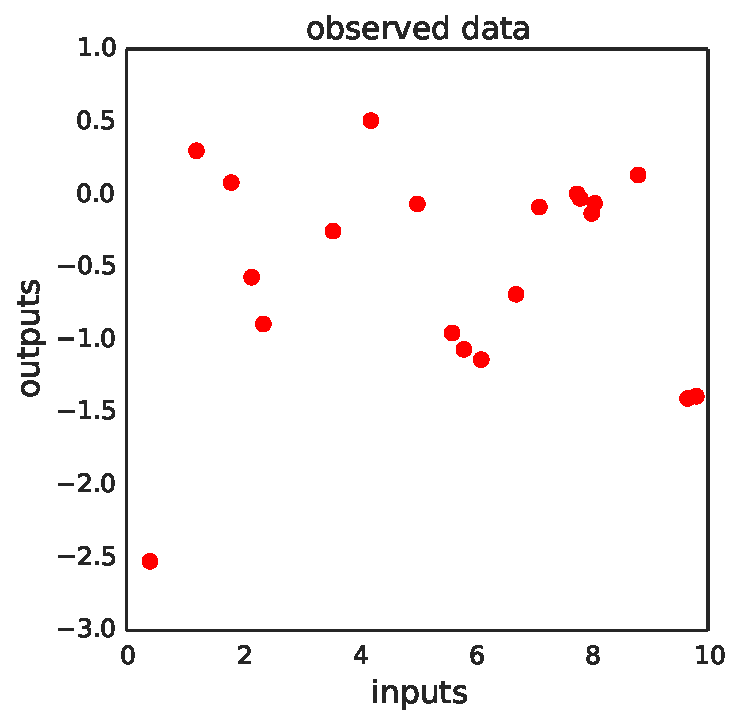
\includegraphics[width=0.24\textwidth]{reg_1}
	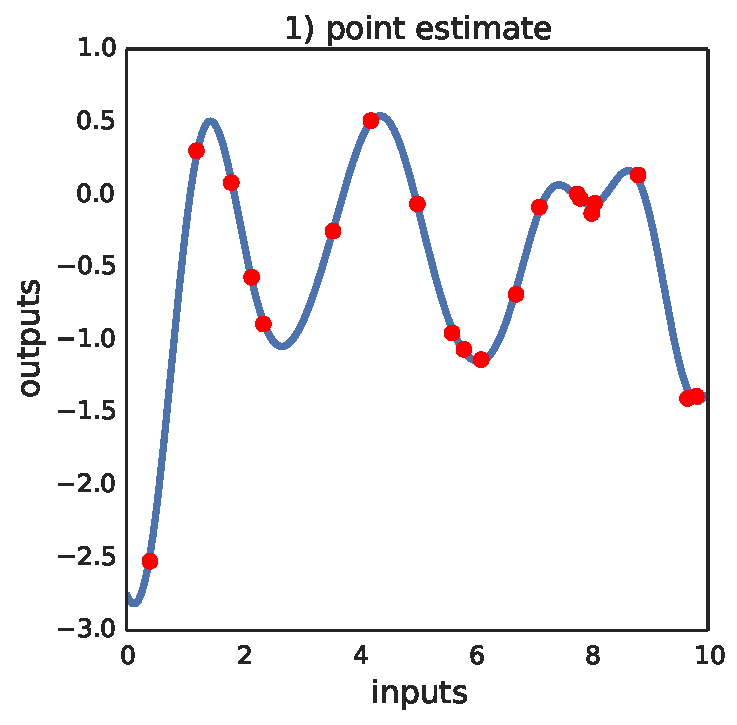
\includegraphics[width=0.24\textwidth]{reg_2}
	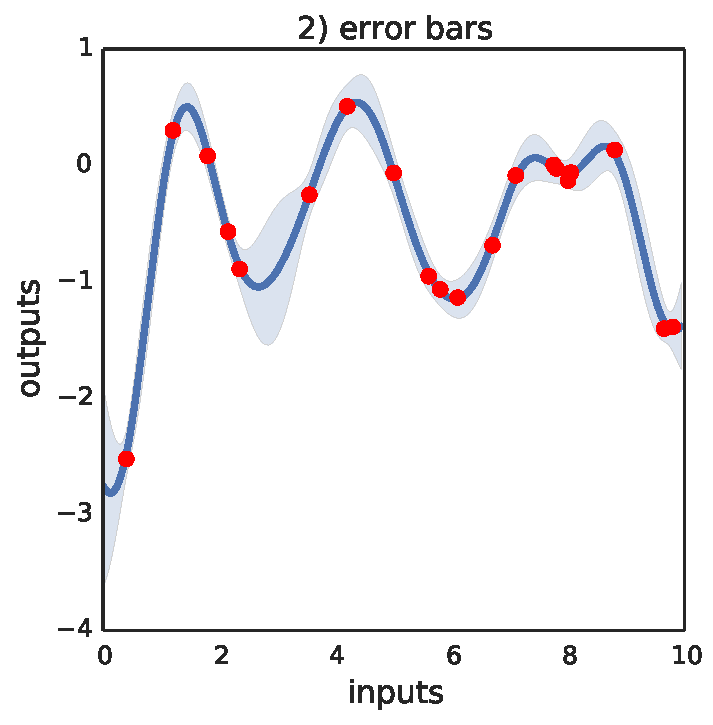
\includegraphics[width=0.24\textwidth]{reg_3}
	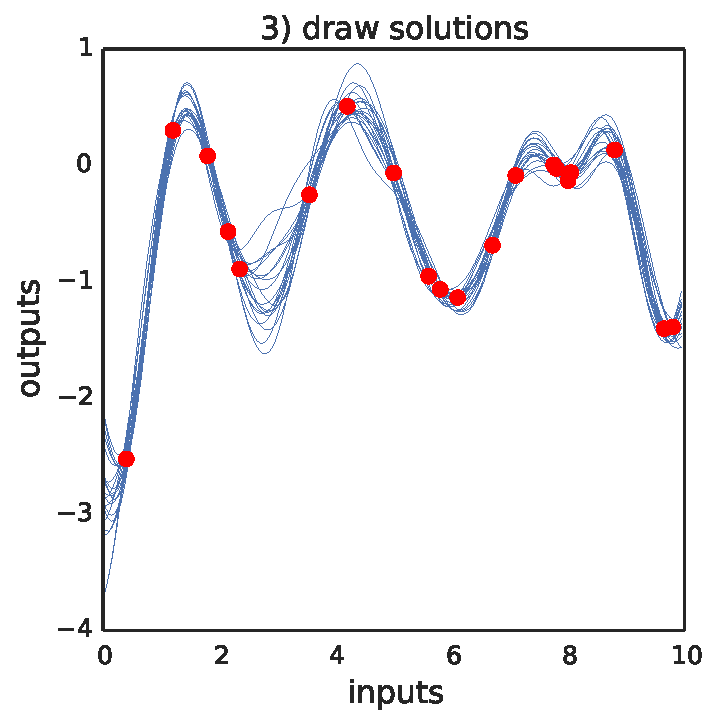
\includegraphics[width=0.24\textwidth]{reg_4}
	\caption{De izquierda a derecha, se muestran datos, estimaciones puntuales, barras de error, y funciones plausibles.}
	\label{fig:regression_problem}
\end{figure}

\section{Modelos Bayesianos Jerárquicos}
\label{sec:hierarchical}

\begin{figure}[h]
	\centering
	\tikz{ 
		\node[obs] (x) {\(\bfx\)};
		\node[obs, right=of x] (t) {\(\bft\)};
		\node[latent, above=of x, yshift=-0.3cm] (theta) {\(\theta\)};
		\node[latent, above=of theta, yshift=-0.3cm] (omega) {\(\omega\)};
		\edge {omega} {theta};
		\edge {theta, t} {x};
		% Plates
		\plate[inner sep=0.3cm, yshift=0.2cm]  {xt} {(t)(x)} {\(\calD\)};
	}
	\hspace{5em}
	\tikz{
		\node[obs] (x) {\(\bfx\)};
		\node[obs, right=of x] (t) {\(\bft\)};
		\node[det, above=of x, yshift=-0.3cm] (theta) {};
		\node[latent, above=of theta, yshift=-0.3cm] (omega) {\(\omega\)};
		\edge {omega} {theta};
		\edge {theta, t} {x};
		% Plates
		\plate[inner sep=0.3cm, yshift=0.2cm]  {xt} {(t)(x)} {\(\calD\)} ;
	}
	\caption{Izquierda: representación gráfica de un modelo bayesiano jerárquico para regresiones, con \emph{hiperparámetros} \(\omega\), \emph{parámetros} \(\theta\) y datos de entrada/salida \(\bft, \bfx\). Derecha: representación gráfica del mismo modelo bayesiano jerárquico, pero integrando los parámetros \(\theta\).}
	\label{fig:hierarchical_model}
\end{figure}

Un \emph{modelo bayesiano jerárquico} está escrito en múltiples etapas o niveles, donde toda la incertidumbre está modelada en términos probabilísticos y se permite utilizar el teorema de Bayes entre dichas etapas de diferente nivel de abstracción. 

Dado un espacio de modelos parametrizado \(\calM = \calI(\Theta)\), consideremos \(p(\theta) \in \calP(\Theta)\) una distribución a priori sobre los parámetros. Si este prior está a la vez parametrizado por \(\omega \in \Omega\), llamados \emph{hiperparámetros}, entonces podemos fijar un \emph{hiperprior} \(p(\omega) \in \calP(\Omega)\) sobre ellos. 

En principio, se puede iterar el proceso: si el hiperprior a su vez tiene parámetros, a estos se les puede llamar hiper-hiperparámetros, y así. Sin embargo, en algún punto debemos parar. 

En la Fig. \ref{fig:hierarchical_model} (izquierda), se presenta un esquema de regresión de dos etapas, donde \(\calD = (\bft, \bfx)\) son datos de entrada/salida y la distribución conjunta es \[p(\bfx, \bft, \theta, \omega) = p(\bfx, \bft \mid \theta, \omega) p(\theta \mid \omega) p(\omega).\]

Fijando un prior \emph{no informativo} sobre \(\bft\), es decir, \(p(\bft \mid \theta, \omega) \propto 1\), con esto la distribución posterior de los parámetros \(\theta\) dado \(\bft,\bfx,\omega\) está dada por
\begin{equation*}
	p(\theta \mid \bfx, \bft, \omega) = \frac{p(\bfx \mid \bft, \theta, \omega) p(\theta \mid \omega)}{p(\bfx \mid \bft, \omega)},
\end{equation*}
donde \(p(\bfx \mid \bft, \theta, \omega) \) es la verosimilitud de \(\theta\), \(p(\theta \mid \omega)\) es el prior de \(\theta\) y la verosimilitud marginal es
\begin{equation*}
	p(\bfx \mid \bft, \omega) = \int_{\Theta} p(\bfx \mid \bft, \theta, \omega) p(\dd{\theta \mid \omega}).
\end{equation*}

Para un hiperparámetro fijo \(\omega\), podemos entrenar el modelo parametrizado por \(\theta\) con cualquier estimador de Bayes, como el máximo a posteriori \(\hat{\theta}_{\mathrm{MAP}} \in \argmax_{\theta \in \Theta} p(\theta \mid \bfx, \bft, \omega)\) o la media posterior \(\hat{\theta}_{l_2} = \int_{\Theta} \theta p(\dd{\theta \mid \bfx, \bft, \omega})\). Adicionalmente, en el contexto de los modelos bayesianos jerárquicos, podemos calcular la \emph{distribución predictiva posterior} de \(\bfxo\) para nuevas entradas \(\bfto\), que está dada por
\begin{equation*}
	p(\bfxo \mid \bfto, \bfx, \bft, \omega) = \int_{\Theta} p(\bfxo \mid \bfto, \theta, \omega) p(\dd{\theta \mid \bfx, \bft, \omega}),
\end{equation*}
que coincide con el \emph{modelo bayesiano promedio} en \(\theta\), es decir
\begin{align}
	\bar m(\bfxo \mid \bfto, \omega)	&= \int_{\Theta} m_{\theta}(\bfxo \mid \bfto, \omega) p(\dd{\theta \mid \bfx, \bft, \omega}) \nonumber \\
										&= \int_{\Theta} p(\bfxo \mid \bfto, \theta, \omega) p(\dd{\theta \mid \bfx, \bft, \omega}) \nonumber\\
										&= p(\bfxo \mid \bfto, \bfx, \bft, \omega).
\end{align}

Notemos que el \emph{modelo bayesiano promedio} \(\bar{m}(\bfxo \mid \bfto, \omega)\) depende solo de \(\omega\), dado que \emph{desintegramos} el parámetro \(\theta\), por lo que debemos \emph{escoger} el hiperparámetro \(\omega\). Para esto, siguiendo el paradigma bayesiano ilustrado en la Figura \ref{fig:hierarchical_model} (derecha), calculamos la distribución posterior de \(\omega\) dado \(\bft, \bfx\) como sigue:
\begin{equation*}
	p(\omega \mid \bfx, \bft) = \frac{p(\bfx \mid \bft, \omega) p(\omega)}{p(\bfx \mid \bft)},
\end{equation*}
donde \(p(\bfx \mid \bft, \omega)\) es la \emph{verosimilitud} de \(\omega\) (a tono con la verosimilitud marginal relacionada a \(\theta\)), \(p(\omega)\) es el prior de \(\omega\) y \(p(\bfx \mid \bft)\) es la verosimilitud marginal relacionada a \(\omega\).

Dado \(p(\omega \mid \bfx, \bft)\), también podemos escoger el modelo (hiper-)parametrizado por \(\omega\) con cualquier estimador de Bayes. En la etapa de hiperparámetros, es normal usar el estimador máximo a posteriori \(\hat{\omega}_{\mathrm{MAP}}\), denotado MAP-II para diferenciarlo del estimador del parámetro MAP \(\hat{\theta}_{\mathrm{MAP}}\), el cual denotamos MAP-I. La razón de esto es que es más común tener posteriores de \(\omega\) más puntiagudas, es decir concentradas en torno a un punto, que usualmente coincide con el MAP-II.

El hecho de integrar los parámetros es lo que distingue el enfoque bayesiano de inferencia con respecto a los enfoques basados en optimización, ya que la verosimilitud marginal incorpora un equilibrio entre ajuste y complejidad.

Si queremos un estimador de Bayes diferente, como el \emph{modelo promedio de hiperparámetros}, nos enfrentamos a un posible problema: las integrales con respecto a \(p(\omega \mid \bfx, \bft)\) son intratables. Sin embargo, podemos aproximarlas por muestras de la distribución usando métodos bayesianos de muestreo, que veremos en la siguiente sección.

El marco teórico introducido se utiliza ampliamente para definir modelos \emph{no paramétricos}, es decir, modelos sin un número fijo de parámetros y que pueden crecer con los datos. Podemos distinguir un modelo no paramétrico que tiene muchas propiedades matemáticas que lo hacen versátil y flexible, especialmente para trabajos de regresión basadas en la distribución gaussiana.

\section{Inferencia Bayesiana}
\comment{explicar la intuición de por que queremos estimar esa integral}
Como vimos en las secciones anteriores, estamos interesados en calcular integrales con respecto a la distribución posterior de parámetros \(p_n(\theta) = \frac{p(x_1,\dots, x_n \mid \theta) p(\theta)}{p(x_1, \dots, x_n)}\), donde la constante de normalización o \emph{evidencia} \(p(x_1, \dots, x_n)\) desconocemos inicialmente. Los métodos de Monte Carlo son un conjunto de métodos no deterministas que nos ayudan a calcular las integrales deseadas, ya que tienen como objetivo resolver los siguientes problemas:
\begin{enumerate}
	\item Dada una variable aleatoria \(X : \Omega \to \reals\), generar un conjunto \(\{X^i\}_{i=1}^N\) de \(N\) muestras.
	\item Dada la función de densidad de probabilidades \(p(x)\) de \(X\) y una función \(g : X(\Omega) \to \reals\), calcular la esperanza de \(g\) con respecto a \(X\):
	\begin{equation*}
	\Phi = \mean_{X}(g) = \int_\Omega g(X(\omega)) \dd{\prob(\omega)} = \int_\reals g(x) p(x) \dd{x}.
	\end{equation*}
\end{enumerate}

Se puede observar que si pudiéramos generar el conjunto \(\{X^i\}_{i=1}^N\) de muestras de \(X\), entonces podríamos estimar la esperanza de \(g\) con respecto a \(X\) como:
\begin{equation*}
\hat{\Phi}=\frac{1}{N} \sum_{i=1}^N g(X^i).
\end{equation*}
Gracias al Teorema del Límite Central \comment{ref al marco teorico}, el estimador \(\hat{\Phi}\) sigue una distribución normal con media \(\Phi\) y con una varianza que decrece en \(O(\frac{1}{N})\):
\begin{equation*}
\hat{\Phi}\sim \calN\left(\Phi, \frac{\mean_{X}((g(X) - \Phi)^2)}{N}\right).
\end{equation*}
La dificultad radica en poder generar muestras de \(X\), ya que en vez de tener \(p(x)\) típicamente se conoce otra función \(p^{\ast}(x)\) que cumple que \(p(x) = \frac{p^{\ast}(x)}{Z}\), donde \(Z\) es una constante de normalización desconocida (como la \emph{evidencia} en el caso de cálculo de posteriores), por lo que no es obvio cómo resolver el problema. Además, la cantidad de muestras necesarias para recorrer todo el espacio crece de forma exponencial en la dimensión de \(X\), por lo que algoritmos «ingenuos» no pueden aplicarse.

\subsection{Rao-Blackwellización}
\comment{extender un poco más la explicación}
Si la dimensión de \(X(\Omega)\) es muy grande, entonces la varianza del estimador crece exponencialmente. Una idea es dividir las variables en dos conjuntos \(X = X_S \cup X_E\), donde \(X_S\) se aproxima a través de muestras \(X_S^1, \dotsc, X_S^n\) y la esperanza con respecto a \(X_E\) dado \(X_S\) se realiza de forma analítica:
\begin{equation*}
\mean_{X}(f) \approx \frac{1}{N} \sum_{i=1}^N \mean_{X_E \mid X_S^i}(f(X_E, X_S^i)).
\end{equation*}

Siendo un poco más explícitos, se tiene que
\begin{align*}
\mean_{X}(f)	&= \int f(x) p(x) \dd{x}\\
&= \iint f(x_S, x_E) p(x_S, x_E) \dd{x_S} \dd{x_E}\\
&= \iint f(x_S, x_E) p(x_S) p(x_E \mid x_S) \dd{x_S} \dd{x_E}\\
&= \int p(x_S) \left[\int f(x_S, x_E) p(x_E \mid x_S) \dd{x_E}\right] \dd{x_S}\\
&= \int p(x_S) \mean_{X_E \mid x_S} (f(X_E, x_S)) \dd{x_S}\\
&\approx \frac{1}{N}\sum_{i=1}^N \mean_{X_E \mid X_S^i} (f(X_{E},X_{S}^{i})).
\end{align*}

A continuación vamos a mostrar diferentes métodos de Monte Carlo para resolver los problemas planteados anteriormente.

\subsection{Muestreo por Rechazo}
Un método a considerar consiste en tener una densidad propuesta \(q(x) = \frac{q^{\ast}(x)}{Z_q},\) de la cual podemos obtener muestras, evaluar \(q^{\ast}(x)\), y conocemos el valor de una constante \(C\) tal que para todo \(x\) en el dominio de \(q\), se tiene que \(C q^{\ast}(x) > p^{\ast}(x)\) La idea se basa en generar una muestra \(\bar{X}\) desde la densidad propuesta \(q(x)\), evaluamos \(C q^{\ast}(\bar{X})\) y generamos una muestra \(u\) a partir de una distribución uniforme en el intervalo \([0, C q^{\ast}(\bar{X})].\) Finalmente evaluamos \(p^{\ast}(\bar{X})\). Si \(u > p^{\ast}(\bar{X})\) entonces \(\bar{X}\) es rechazado, y en caso contrario es aceptado. Este método se conoce como muestreo por rechazo, o \emph{rejection sampling} en inglés.

\begin{proposition}
	Sean \(\bar{X} \sim q(x)\) y \(u \sim U([0,Cq^\ast(\bar{X})])\). Si \(u \leq p^\ast(\bar{X})\) entonces \(\bar{X} \sim p(x)\).
\end{proposition}

\begin{figure}[h]
	\centering
	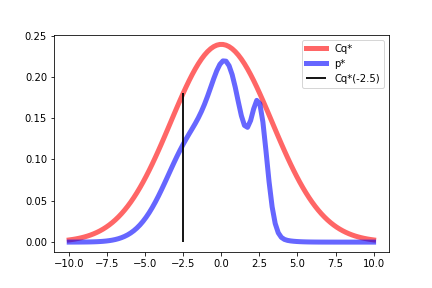
\includegraphics[scale=0.7]{rejection_sampling}
	\caption{Representación gráfica del algoritmo: se samplea un valor para \(\bar{X}\) usando \(q\) y se samplea una uniforme sobre la linea negra, que va desde el 0 hasta \(Cq^\ast(\bar{X})\), y si cae dentro del área de \(p*\) entonces el \(\bar{X}\) es aceptado como muestra de \(p\).}
	\label{fig:rejection_sampling}
\end{figure}
El problema con este método, es que \(q(x)\) debe ser una buena aproximación de \(p(x)\), ya que en caso contrario la constante \(C\) será muy grande y, por ende, la frecuencia de rechazo será muy grande. Además, la constante crece de forma exponencial con el tamaño de la dimensión de \(X(\Omega)\), por lo que no puede ser utilizado en grandes dimensiones.

\subsection{Muestreo por Importancia}

El método muestreo por importancia (llamado \emph{importance sampling} en inglés) no es un método para generar muestras, sino que para estimar la esperanza de una función \(f\) con respecto a \(p(x) = \frac{p^{\ast}(x)}{Z}\), donde solo podemos evaluar \(p^{\ast}(x)\). Supongamos que tenemos una densidad propuesta \(q(x) = \frac{q^{\ast}(x)}{Z_q}\), de la cual podemos obtener muestras y evaluar \(q^{\ast}(x)\). Si \(q(x) > 0\), entonces se cumple la siguiente igualdad: 
\begin{equation*}
\mean_{X}(f) = \int f(x) p(x) \dd{x} = \int f(x) \frac{p(x)}{q(x)} q(x) \dd{x} = \mean_{q}\left(f\frac{p}{q}\right).
\end{equation*}

\begin{figure}[h]
	\centering
	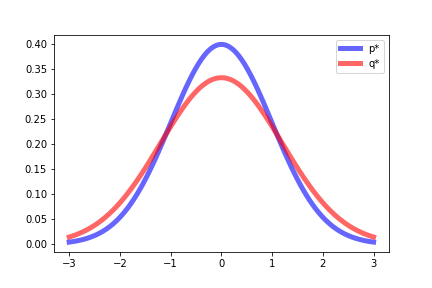
\includegraphics[scale=0.7]{important_sampling}
	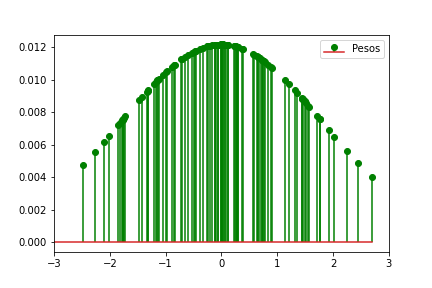
\includegraphics[scale=0.7]{important_sampling_w}
	\caption{Arriba: Las funciones de densidad de distribución objetivo \(p*(x)\) y propuesta \(q*(x)\). Abajo: Los pesos de muestras (samples) de \(q(x)\).}
	\label{fig:important_sampling}
\end{figure}

Sean \(\{X^i\}_{i=1}^N\) \(N\) muestras de \(q(x)\), y definamos sus \emph{pesos} como
\begin{equation*}
w_i = \frac{p^{\ast}(X^i)}{q^{\ast}(X^i)},
\end{equation*}
con los cuales ajustamos la \emph{importancia} de cada punto en nuestro estimador
\begin{equation*}
\hat{\Phi} = \sum_{i=1}^N \frac{w_i}{\sum_{j=1}^N w_j} f(X^i).
\end{equation*}
Para que nuestro estimador \(\hat{\Phi}\) converja a \(\Phi\), es necesario que se cumpla que para todo \(x\), \(p(x) > 0 \implies q(x) > 0\). Idealmente, \(q(x)\) debe parecerse lo más posible a \(p(x)\), incluso en las colas, que deben decrecer a una velocidad similar. El gran problema de este método es que el rango de los pesos \(w_i\) es exponencial a la raíz cuadrada de la dimensión de \(X(\Omega)\):
\begin{equation*}
\frac{w^{\max}}{w^{\mathrm{med}}} = O(\exp(\sqrt{\dim(X(\Omega))})),
\end{equation*}
por lo que la estimación estará dominada por unas pocas muestras con gran peso.

\subsection{Cadenas de Markov de Monte Carlo (MCMC)}

Los métodos anteriores tienen sus ventajas en casos simples, pero su principal desventaja es que no se comportan bien para distribuciones de gran dimensión, ya que es difícil construir una distribución propuesta similar a la distribución objetivo en todas sus dimensiones. 

Un enfoque diferente al problema de inferencia se basa en el mecanismo de cadenas de Markov, en donde los \emph{estados} de la cadena son los conjuntos de valores de las variables a muestrear, y con una función de \emph{transición} de probabilidades adecuada entre estos se procede a muestrear los valores de la cadena. Luego de un cierto tiempo conocido como \emph{burn-in time}, la simulación converge a una distribución \emph{estacionaria} que coincide con la distribución objetivo.

Formalicemos todos estos conceptos a continuación. Por abuso de notación, si el espacio de estados \(\calX\) es discreto o continuo, entonces \(\prob\) denotará la función de masa o de densidad respectivamente.
\begin{definition}
	Una cadena es un proceso estocástico a tiempo discreto con valores en \(\calX\), es decir \((X_n)_{n \in \naturals}\). Decimos que la cadena es de Markov si cumple que para cualquier valor en sus estados \(x_0, x_1, \dotsc, x_n, x_{n+1} \in \calX\) se satisface que
	\[\prob(X_{n+1} = x_{n+1} \mid X_n = x_n, \dotsc, X_0 = x_0) = \prob(X_{n+1} = x_{n+1} \mid X_n = x_n).\]
\end{definition}
Se dice que una cadena de Markov es homogénea si la probabilidad de pasar de un estado a otro, en un paso, no depende del tiempo en que se encuentre la cadena, es decir,
\[\prob(X_{n+1} = b \mid X_n = a) = \prob(X_1 = b \mid X_0 = a) = T(a, b).\]
El kernel \(T\) cumple con que \(T(a, b) \geq 0\) y \(\int_{\calX} T(a, x) \dd{x} = 1\) para todo \(a, b \in \calX\).

Así como \(T(a, b)\) es la probabilidad de llegar desde el estado \(a\) al estado \(b\) en un paso, \(T^n(a, b)\) es la probabilidad de llegar desde el estado \(a\) al estado \(b\) en \(n\) pasos. Notemos que \(T^2(a,b) = \int_\calX T(a, x) T(x, b) \dd{x}\) y \(T^n(a,b) = \int_\calX T^{n-1}(a, x) T(x, b) \dd{x}\).

Diremos que dos estados \(a, b \in \calX\) se comunican si existen \(n_1, n_2 \in \naturals\) tales que \(T^{n_1}(a, b) > 0\) y \(T^{n_2}(b, a) > 0\). Si todos los estados se comunican entre sí, entonces diremos que la cadena es irreducible.

El periodo de un estado \(a \in \calX\) se define como \(d(a) = \mathrm{mcd}\{n \geq : T^n(a, a) > 0\}\), donde \(\mathrm{mcd}\) denota el máximo común divisor. Si \(d(a) = 1\) diremos que el estado \(a\) es aperiódico, y si todos los estados son aperiódicos entonces se dice que la cadena es aperiódica.

La última propiedad de una cadena de Markov que vamos a introducir es la recurrencia positiva. El tiempo medio de recurrencia de un estado \(j\) a partir del estado \(i\) se define como el siguiente valor esperado:
\[\mu_{i, j} = \mean(\min\{n \geq 1 : X_n = j \mid X_0 = i\}).\]
Si \(\mu_{i, i}\) es finito, entonces se dice que \(i\) es recurrente positivo, y si todos los estados son recurrentes positivos entonces se dice que la cadena es recurrente positiva.

Denotemos por \(\pi = (\pi_i)_{i\in\calX}\) a una distribución de probabilidad sobre \(\calX\). Se dice que \(\pi\) es una distribución estacionaria para una cadena de Markov con kernel de \(T\) si se cumple que para \(y \in \calX\),
\[\pi_j = \int_{\calX}T(x, j) \pi_x \dd{x}.\]
Si la cadena de Markov es homogénea con kernel de transición \(T\), irreducible, aperiódica y recurrente positiva, entonces la cadena tiene una única distribución estacionaria \(\pi\) tal que para todo \(i \in \calX\) se tiene que
\[\lim_{n \to \infty} T^n(i, j) = \pi_j.\]

El resultado anterior quiere decir que, dada una distribución de probabilidad \(\prob\), si somos capaces de construir una cadena de Markov con kernel de transición \(T_\prob\) tal que su distribución estacionaria sea \(\prob\), entonces después de simular por un tiempo conocido como \emph{burn-in}, partiendo desde cualquier punto una simulación termina muestreando desde \(\prob\). Veamos a continuación los métodos de MCMC más utilizados.

\subsection{Metropolis-Hasting}

Sea \(\prob(X)\) la distribución de probabilidad de la cual se quiere muestrear \(X = \{x_1, \dotsc, x_n\}\), y sea \(Q(x^{\ast}; x)\) una distribución propuesta para muestrear un valor candidato \(x^{\ast}\) desde el valor actual \(x\).
\begin{figure}[h]
	\centering
	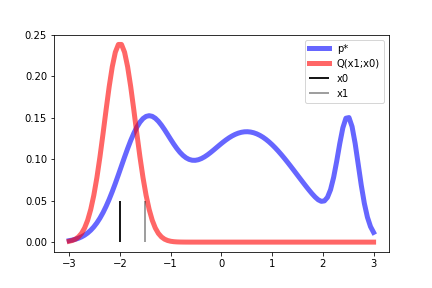
\includegraphics[scale=0.5]{MH1}
	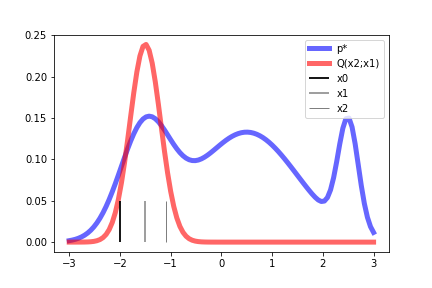
\includegraphics[scale=0.5]{MH2}
	\caption{Izquierda: Primera iteración del método Metropolis-Hasting. Derecha: Segunda iteración del método Metropolis-Hasting.}
	\label{fig:MH}
\end{figure}
Construimos una cadena de Markov que se mueve desde el estado \(x\) al estado \(x^{\ast}\) con una probabilidad de aceptación dada por
\begin{equation*}
A(x, x^{\ast}) = \min \left\{1, \frac{\prob(x^{\ast}) Q(x; x^{\ast})}{\prob(x) Q(x^{\ast}; x)} \right\}.
\end{equation*}
y en caso contrario permanece en \(x\). El algoritmo es muy simple, pero depende completamente de la distribución propuesta \(Q\). A continuación se muestra el seudocódigo del algoritmo general.

\begin{algorithm}[h]
	\caption{Metropolis-Hastings}
	\begin{algorithmic}[1]
		\State Inicializar \(x^{(0)}\).
		\For{\(i = 0, \dotsc, N-1\)}
		\State Muestrear \(u \sim \calU(0, 1)\).
		\State Muestrear \(x^{\ast} \sim Q(x^{\ast}; x^{(i)})\)
		\If{\(u < A(x^{(i)}, x)\)}
		\State \(x^{(i + 1)} \gets x^{\ast}\).
		\Else
		\State \(x^{(i + 1)} \gets x^{(i)}\).
		\EndIf
		\EndFor
	\end{algorithmic}
\end{algorithm}

Para demostrar que este algoritmo converge a la distribución objetivo \(\prob\) basta con demostrar que la cadena construida tiene un kernel de transición \(T\) tal que:
\begin{align*}
T(x, y)				&= Q(y; x) A(x, y),\\
T(x, y) \prob(x)	&= T(y, x) \prob(y).
\end{align*}

En efecto,
\begin{enumerate}
	\item Si \(Q(y; x) \prob(x) = Q(x; y) \prob(y)\), entonces \(A(x, y) = A(y ,x) = 1\) por lo que \(T(x, y) \prob(x) = T(y, x)\prob(y)\).
	
	\item Si \(Q(y; x) \prob(x) > Q(x; y) \prob(y)\), entonces
	\[A(x, y) = \frac{Q(x; y) \prob(y)}{Q(y; x) \prob(x)},\]
	y \(A(y, x) = 1\), lo que implica que
	\begin{align*}
	T(x, y) \prob(x)	&= Q(y; x) A(x, y) \prob(x)\\
	&= Q(y; x) \frac{Q(x; y) \prob(y)}{Q(y; x) \prob(x)} \prob(x)\\
	&= Q(x; y) \prob(y)\\
	&= Q(x; y) A(y, x) \prob(y)\\
	&= T(y, x)\prob(y).
	\end{align*}
	\item Si \(Q(y; x) \prob(x) < Q(x; y) \prob(y)\), entonces \(A(x, y) = 1\) y
	\[A(y, x) = \frac{Q(y; x) \prob(x)}{Q(x; y) \prob(y)},\]
	lo que implica que
	\begin{align*}
	T(y, x) \prob(y)	&= Q(x; y) A(y, x) \prob(y)\\
	&= Q(x; y) \frac{Q(y; x) \prob(x)}{Q(x; y) \prob(y)} \prob(y)\\
	&= Q(y; x) \prob(x)\\
	&= Q(y; x) A(x, y) \prob(x)\\
	&= T(x,y) \prob(x).
	\end{align*}
\end{enumerate}

En el caso particular en que \(Q(y; x)\) es simétrica, entonces el algoritmo se conoce como simplemente \emph{Metropolis} y el cambio es que la función de aceptación es de la forma
\begin{equation*}
A(x^{(i)}, x^{\ast}) = \min \left\{1, \frac{\prob(x^{\ast})}{\prob(x^{(i)})}\right\}.
\end{equation*}

La principal gracia de los métodos de MCMC es que para simular debemos calcular la razón entre las probabilidades \(\prob(x^{\ast})\) y \(\prob(x^{(i)})\), por lo que si tenemos una versión no normalizada \(\hat{\prob}\), la constante de normalización se simplifica al calcular dicha razón, es decir,
\[\frac{\hat{\prob}(x^{\ast})}{\hat{\prob}(x^{(i)})} = \frac{\prob(x^{\ast})}{\prob(x^{(i)})}.\]

\subsection{Muestreo de Gibbs}

Sea \(X = \{x_1, \dotsc, x_n\}\) y definamos \(x_{-i} = X \setminus \{x_i\}\). Supongamos que es posible calcular \(\prob(x_i \mid x_{-i})\) para todo \(i = 1, \dotsc, n\). En ese caso definamos la distribución propuesta
\[ Q(x^{\ast}; x^{(i)}) = \begin{dcases*}
\prob(x_j^{\ast} \mid x_{-j}^{(i)})	& si \(x_{-j}^{\ast} = x_{-j}^{(i)}\),\\
0									& en caso contrario.
\end{dcases*} \]

El Muestreo de Gibbs es el caso particular de Metropolis-Hasting, con la distribución recién definida, y cumple que su probabilidad de aceptación es:
\begin{align*}
A(x^{(i)}, x^{\ast})	&= \min \left\{1, \frac{\prob(x^{\ast})Q(x^{(i)}; x^{\ast})}{\prob(x^{(i)}) Q(x^{\ast}; x^{(i)})} \right\}\\
&= \min \left\{1, \frac{\prob(x^{\ast}) \prob(x_j^{(i)} \mid x_{-j}^{(i)})}{\prob(x^{(i)}) \prob(x_j^{\ast} \mid x_{-j}^{\ast})} \right\}\\
&= \min \left\{1, \frac{\prob(x_{-j}^{\ast})}{\prob(x_{-j}^{(i)})} \right\}\\
&= 1.
\end{align*}
Esto quiere decir que todo algoritmo que muestree generado en cada iteración es aceptado. La selección de la variable a muestrear se puede hacer de forma ordenada o de forma aleatoria. A continuación mostramos el algoritmo para el caso ordenado:
\begin{algorithm}[h]
	\caption{Muestreo de Gibbs Ordenado}
	\begin{algorithmic}[1]
		\State Inicializar \(x^{(0)}\).
		\For{\(i = 0, \dotsc, N-1\)}
		\For{\(j = 1, \dotsc n\)}
		\State Muestrear \(x_j^{(i+1)} \sim \prob(x_j \mid x_{-j}^{(i)})\).
		\EndFor
		\EndFor
	\end{algorithmic}
\end{algorithm}

En \cite{green1995reversible} se propone un método MCMC aplicado a la modelación bayesiana, que permite saltar de dimensión en la cantidad de parámetros de la cadena, lo que es muy útil si no se conocen a priori la cantidad de parámetros a estimar. En \cite{murray2008gaussian} se presenta un método de MCMC en donde se modela una distribución utilizando un GP auxiliar, permitiendo así modelar las distribuciones de forma bayesiana y no paramétrica.
\comment{seccion: quizas falta un ejemplo simplecito para entender}

\comment{parrafo: pequeña reseña y aterrizado de lo enseñado}

\comment{parrafo: dado que es un tema bien conocido por donzas, un parrafo motivando otras lecturas y menciones del estado del arte.}

\subsection{Inferencia Variacional}

\comment{Parrafo: contexto, mostrarlo como una alternativa a MCMC}

Las técnicas de inferencia variacional se basan en aproximar la distribución condicional \(p(\theta \mid X)\) utilizando una distribución variacional \(q(\theta)\) que maximice la similitud con la distribución\ \(p(\theta \mid X)\) con el criterio de la divergencia de Kullback-Leibler, de forma que
\begin{equation*}
\argmin_{q} \KL (q \parallel p(\cdot \mid X)) = \int  \ln \left(\frac{q(\theta)}{p(\theta \mid X)}\right) q(\theta)\dd{\theta}.
\end{equation*}
Se puede comprobar la siguiente relación:
\begin{equation*}
\ln p(X) = \KL (q \parallel p(\cdot \mid X)) + F(q, X).
\end{equation*}
Luego, para minimizar \(\KL\) se debe maximizar la energía libre \(F\):
\begin{equation*}
F(q, X) = \int q(\theta) \ln \left(\frac{p(\theta, X)}{q(\theta)}\right) \dd{\theta} = \left\langle \ln p(\cdot, X) \right\rangle_{q} + H(q),
\end{equation*}
donde \(H(q)\) es la entropía de \(q\), y \(\left\langle \ln p(\theta,X) \right\rangle_q\) es la \emph{expected log-joint}. 

Un ejemplo simple es la conocida aproximación de Laplace, que se describe a continuación:
\begin{align*}
\theta^{\ast}	&= \argmax_{\theta} \ln p(\theta,X),\\
\Lambda			&= \nabla_\theta \nabla_\theta \ln p(\theta^{\ast},X),\\
q(\theta)		&\sim \calN(\theta \mid \theta^{\ast}, \Lambda^{-1}).
\end{align*}
Se puede revisar \cite{titsias2009variational}, \cite{gal2014variational}, y \cite{matthews2016sparse} para profundizar en el tema de las aplicaciones de inferencia variacional a procesos gaussianos.
\comment{expandir más este ultimo parrafo, motivando la lectura de otras cosas asi como avances recientes, la idea es que el libro tambien pueda ser una guia a los que quieran profundizar más.}
	%!TEX root = main.tex

\chapter{Procesos Gaussianos de Regresión}
\label{sec:gaussian}

\begin{chapquote}{Gabriel Lippmann a Henri Poincaré, sobre la distribución gaussiana}
	``Los experimentalistas piensan que es un teorema matemático mientras que los matemáticos creen que es un hecho experimental.''
\end{chapquote}

En los capítulos anteriores definimos todos los elementos necesarios para llegar a definir los procesos gaussianos desde un punto de vista como modelos de regresión. Sin embargo, aún no es claro el por qué de usar estos objectos matemáticos en la tarea de regresión ni como hacerlo. En este capítulo vamos a profundizas en ambas preguntas para responderlas y quede claro la razón del porqué y cómo.

\comment{parrafo: explicando la motivación y por que son importantes, usos, intuición asi como propiedades bonitas}

\comment{parrafo: resumen y guia del capitulo}

\section{Modelos de Regresión}

En las siguientes secciones vamos a hacer una construcción incremental del modelo conocido como una \emph{regresión de procesos gaussianos}. Vamos a partir definiendo el modelo de regresión lineal más simple, para luego ir agregándole complejidad al modelo y deducir así un modelo de regresión no lineal, bayesiano y no paramétrico, coincidiendo con los procesos gaussianos.

\begin{figure}[h]
	\centering
	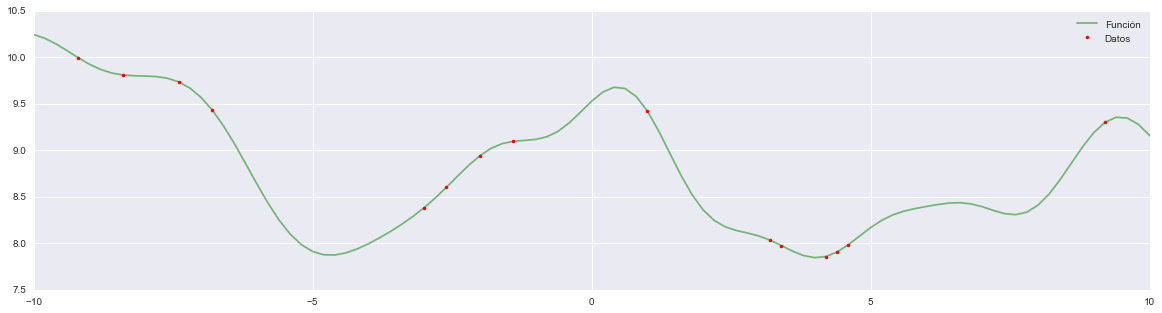
\includegraphics[scale=0.4]{regression}
\end{figure}

Para definir los diferentes modelos de regresión \(f(t) = x\), introduciremos la notación para denotar los conjuntos de datos que serán utilizados en la estimación de los parámetros del modelo. Sea \(\calD = \{(t_i, x_i)\}_{i = 1, \dotsc, n}\) el conjunto de \(n\) pares de datos que se observaron de las variables \((t, x)\), donde \(t = (t^{(1)}, \dotsc, t^{(d)}) \in \calT \subseteq \reals^{1 \times d}\) denota la variable de entrada (variable independiente) e \(x \in \calX \subseteq \reals\) denota la variable de salida (variable dependiente o estado). Denotemos \(T_n = [t_1, \dotsc, t_n]^{\top} \in \reals^{n \times d}\) a la matriz de entrada e \(\bfx_n = [x_1, \dotsc, x_n]^{\top} \in \reals^{n \times 1}\) al vector de salida.

Queremos estimar una función \(f\) a partir de los datos \(\calD_n\), de forma que para todo \(i = 1, \dotsc, n\), los valores \(f(t_i)\) sean cercanos a \(t_i\). Para esto vamos a proponer diferentes formas para \(f\), que dependerá de la base de funciones escogidas y los parámetros. La forma más simple es un modelo lineal, que veremos a continuación.

\subsection{Modelo Lineal}

Consideremos el modelo de regresión lineal simple de parámetros \(w \in \reals^{1 \times d}\) en donde
\begin{equation*}
	x = f(t) = \langle t, w \rangle_{\calT} = t w^{\top}.
\end{equation*}%
Notemos que para agregar una constante al modelo lineal, basta con extender el espacio de entrada en una dimensión, de forma que el modelo lineal es sobre la variable \(\tilde{t} = [1, t]\), por lo que la forma paramétrica del modelo se mantiene intacta.

Si tenemos \(n = d\) datos, donde la matriz cuadrada \(T_n\) es de rango completo, entonces \(w\) y \(f\) se obtienen resolviendo el sistema lineal
\begin{align*}
	T_n w^{\top}	&= \bfx_n,\\
	w^{\top}		&= T_n^{-1} \bfx_n,\\
	f(\bar{t})		&= \bar{t} T_n^{-1} \bfx_n.
\end{align*}%
En general, la cantidad de datos \(n\) no es igual a la dimensión de entrada, por lo que el sistema no tiene solución en el caso general. Un enfoque es estimar el \emph{mejor} modelo lineal posible que se ajuste a los datos, y para esto utilizaremos la técnica conocida como mínimos cuadrados, que se basa en resolver el siguiente problema de optimización:
\begin{equation*}
	\min_{w \in \reals^d} \frac{1}{2} \left\Vert \bfx_n - T_n w^{\top} \right\Vert_n^2.
\end{equation*}

\begin{proposition}
	La solución al problema de mínimos cuadrados lineal tiene solución explícita igual a \(w^{\top} = \left(T_n^{\top} T_n\right)^{-1} T_n^{\top} \bfx_n\), siempre y cuando \(T_n^{\top} T_n\) sea de rango completo.
\end{proposition}

El resultado anterior se obtiene directamente de derivar el funcional a minimizar e igualar el jacobiano a cero:
\begin{align*}
	J(w)									&= \frac{1}{2} \left\Vert \bfx_n - T_n w^{\top} \right\Vert_n^2 = \frac{1}{2} \sum_{i=1}^n \left(x_i - t_i w^{\top}\right)^2,\\
	\dv{J}{w}								&= \sum_{i=1}^n - t_i^{\top} \left(x_i - t_i w^{\top}\right) = 0 \in \reals^d,\\
	\sum_{t=1}^n t_i^{\top} t_i w^{\top}	&= \sum_{i=1}^n t_i^{\top} x_i,\\
	T_n^{\top} T_n w^{\top}					&= T_n^{\top} \bfx_n,\\
	w^{\top}								&= \left(T_n^{\top} T_n\right)^{-1} T_n^{\top}\bfx_n,\\
	f(\bar{t})								&= \bar{t} \left(T_n^{\top} T_n\right)^{-1} T_n^{\top}\bfx_n.
\end{align*}


Podemos ver que si \(T_n\) es invertible, entonces \(n = d\) y se reduce a la expresión anterior. La expresión \(\left(T_n^{\top} T_n\right)^{-1} T_n^{\top}\) se conoce como la pseudoinversa de Moore-Penrose de \(T_n\), y se denota como \(T_n^+\), de forma de que la solución se puede reescribir como \(f(\bar{t}) = \bar{t} T_n^+ \bfx_n\). 

\subsection{Modelo Lineal con Ruido}
Consideremos el caso que la variable \(x\) tiene ruido \(\varepsilon\) generado de una fuente aleatoria:
\begin{equation*}
	x = t w^{\top} + \varepsilon.
\end{equation*}%

\begin{figure}[h]
	\centering
	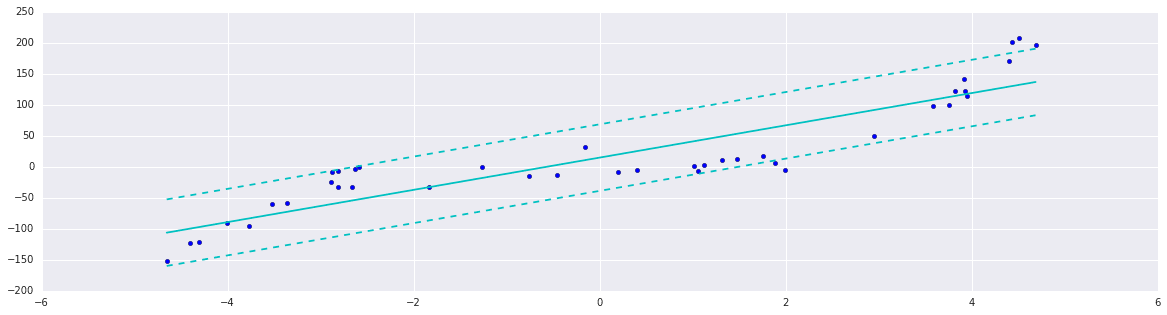
\includegraphics[scale=0.4]{linear}
\end{figure}

Si suponemos que los ruidos (o errores) son independientes e idénticamente distribuidos de forma normal, entonces podemos escribir el modelo de forma que
\begin{align*}
	x_i				&= t_i w^{\top} + \varepsilon_i,\\
	\varepsilon_i	&\sim \calN \left(0, \sigma^2\right),\\
	x \mid t		&\sim \calN \left(t w^{\top}, \sigma^2\right),
\end{align*}
donde \(\sigma^2\) es el parámetro de ruido del modelo. Queremos estimar los parámetros \(w\) y \(\sigma^2\), de modo que el modelo generado sea lo más verosímil posible. La noción de verosimilitud del modelo será modelada como la probabilidad de que los datos hayan sido generadas por el modelo parámetro, es decir,
\begin{equation*}
	\calL \left(w, \sigma^2\right) = p\left(\bfx_n \mid T_n, w, \sigma^2\right),
\end{equation*}
la cual en el caso gaussiano independiente se tiene de forma explícita:
\begin{align*}
	\calL \left(w, \sigma^2\right)	&= \prod_{i=1}^n p\left(x_i \mid t_i, w, \sigma^2\right)\\
									&= \frac{1}{(2\pi)^{\frac{n}{2}} \sigma^n} \exp \left(-\frac{1}{2\sigma^2} \sum_{i=1}^n \left(x_i - t_i w^{\top}\right)^2\right).
\end{align*}

Para maximizar la verosimilitud, podemos aplicar logaritmo a la función objetivo, y si cambiamos el signo entonces tenemos la función de log-verosimilitud negativa, denotada NLL por las siglas en inglés de \emph{negative log-likelihood}, la cual debemos minimizar:
\begin{equation*}
	\ell \left(w, \sigma^2\right) = \frac{n}{2} \ln(2\pi) + n \ln(\sigma) + \frac{1}{2\sigma^2} \sum_{i=1}^n \left(x_i - t_i w^{\top}\right)^2.
\end{equation*}
Podemos ver que la función a minimizar es similar al caso no probabilista, pero con el parámetro \(\sigma\) adicional. Derivando con respecto a los parámetros \(w\) y \(\sigma\) para luego igualar a cero, se obtiene que
\begin{align*}
	\dv{\ell}{w}		&= \frac{1}{\sigma^2} \sum_{i=1}^n - t_i^{\top} \left(x_i - t_i w^{\top}\right) = 0,\\
						&\implies w^{\top} = \left(T_n^{\top} T_n\right)^{-1} T_n^{\top}\bfx_n,\\
	\dv{\ell}{\sigma}	&= \frac{n}{\sigma} - \frac{1}{\sigma^3} \sum_{i=1}^n \left(x_i - t_i w^{\top}\right)^2 = 0,\\
						&\implies \sigma^2 = \frac{1}{n} \sum_{i=1}^n \left(x_i - t_i w^{\top}\right)^2,
\end{align*}
luego la probabilidad predictiva de \(f(x)\) es
\begin{align*}
	p\left(\bar{f} \mid \bar{t}, T_n, \bfx_n\right)	&= \calN \left(\bar{\mu}_{\bar{f}}, \bar{\sigma}_{\bar{f}}^2\right),\\
	\bar{\mu}_{\bar{f}}								&= \bar{t} \left(T_n^{\top} T_n\right)^{-1} T_n^{\top} \bfx_n,\\
	\bar{\sigma}_{\bar{f}}^2						&= \frac{1}{n} \left\Vert \bfx_n - T_n w^{\top} \right\Vert_n^2.
\end{align*}
Podemos ver que los parámetros \(w\) coinciden con el caso no probabilista, pero nos entrega una medida de la varianza del ruido, que coincide con el error cuadrático promedio.

\subsection{Modelo Lineal Bayesiano}

Siguiendo el formalismo bayesiano, es necesario especificar una distribución \emph{a priori} sobre los parámetros \(w\). Consideremos el caso en el que los pesos se distribuyen \emph{a priori} de forma normal con media nula y matriz de covarianza \(\Sigma_{w}\):
\begin{equation*}
	w \sim \calN \left(0, \Sigma_w\right).
\end{equation*}%
Podemos aplicar el Teorema de Bayes para encontrar la distribución \emph{a posteriori} de \(w\) dado los datos observados:
\begin{equation*}
	p(w \mid T_n, \bfx_n) = \frac{p(\bfx_n \mid T_n, w) p(w)}{p(\bfx_n \mid T_n)}.
\end{equation*}
Se puede ver que la función a minimizar es la suma entre la NLL y la log-prior negativa (NLP), la cual en un enfoque no bayesiano se considera como un termino de penalización:
\begin{equation*}
	NLP = \frac{d}{2} \ln(2\pi) + d \ln \left\vert \Sigma_w \right\vert + \frac{1}{2} w \Sigma_w^{-1} w.
\end{equation*}
Si combinamos la distribución a priori \(p(w) = \calN (0, \Sigma_w)\) con la verosimilitud de los parámetros \(p(\bfx_n \mid T_n, w) = \calN \left(T_n w^{\top}, \sigma^2 I_n\right)\) de forma analítica, obtenemos que la distribución a posteriori de \(w\) es normal:
\begin{align*}
	w \mid T_n, \bfx_n	&\sim \calN\left(\Sigma_w^{T_n} T_n^{\top} \bfx_n, \sigma^2 \Sigma_w^{T_n}\right),\\
	\Sigma_w^{T_n}		&= \left(T_n^{\top} T_n + \sigma^2 \Sigma_w^{-1}\right)^{-1}.
\end{align*}
Como su media y su moda coinciden, el estimador máximo a posteriori de \(w\) (denotado MAP por sus siglas en inglés \emph{maximum a posteriori}) es igual a
\begin{align*}
	\hat{w}	&= \Sigma_w^{T_n} T_n^{\top} \bfx_n,\\
			&= \left(T_n^{\top} T_n + \sigma^2 \Sigma_w^{-1}\right)^{-1} T_n^{\top} \bfx_n
\end{align*}

Si observamos nueva evidencia \(\bar{t}\), entonces la distribución predictiva de \(\bar{f} = f(\bar{t})\) esta dada por el promedio de todos los posibles modelos lineales, es decir:
\begin{align*}
	p \left(\bar{f} \mid \bar{t}, T_n,X_n\right)	&= \int p \left(\bar{f} \mid \bar{t}, w\right) p\left(w \mid T_n, X_n\right) \dd{w} = \calN \left(\bar{\mu}_{\bar{f}}, \bar{\sigma}_{\bar{f}}^2\right),\\
	\bar{\mu}_{\bar{f}}								&= \bar{t} \left(T_n^{\top} T_n + \sigma^2\Sigma_w^{-1}\right)^{-1} T_n^{\top} \bfx_n,\\
	\bar{\sigma}_{\bar{f}}^2						&= \sigma^2 \bar{t} \left(T_n^{\top} T_n + \sigma^2 \Sigma_w^{-1}\right)^{-1} \bar{t}^{\top}.
\end{align*}%
En este modelo, la distribución predictiva de \(\bar{y}\) coincide con la de \(\bar{f}\), pero con una varianza mayor (se suma \(\sigma^2)\).

\subsection{Modelo No Lineal Bayesiano}

Un enfoque para aumentar la flexibilidad del modelo es utilizar una proyección \(\phi : \calT \to \calF\) que mapea una variable de entrada \(t \in \reals^{1 \times d}\) a una variable \(\phi(t)\) del espacio \(\calF \subseteq \reals^{1 \times \bar{d}}\) de mayor dimensión \(\bar{d}\), denotado como espacio de características o \emph{feature space}. Si nuestro modelo es lineal en el espacio \(\calF\), entonces el modelo es de la forma
\begin{equation*}
	x = f(t) = \langle \phi(t), w \rangle_{\calF} = \phi(t) w^{\top},
\end{equation*}
donde \(w\) es el vector de parámetros de dimensión \(\bar{d}\) del modelo lineal en las características. Por ejemplo, si \(\phi\) proyecta en el espacio de las potencias de hasta orden \(n\), es decir \(\phi(t) = (1, t, t^2, \dotsc, t^p)\), entonces el modelo lineal en \(\calF\) es equivalente a un modelo polinomial de orden \(p\) en \(\calT\).
\begin{figure}[h]
	\centering
	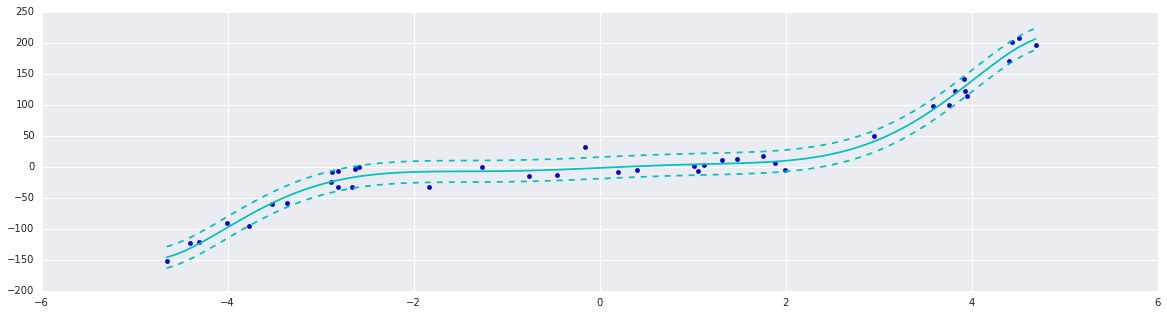
\includegraphics[scale=0.4]{no-linear}
\end{figure}

De esta forma, es directo ver que la fórmula del caso lineal es muy similar a este modelo, en donde cambiamos la variable \(t\) por la variable \(\phi(t)\), obteniendo así que la distribución predictiva de \(\bar{f}\) es normal con media y varianza
\begin{align*}
	p \left(\bar{f} \mid \bar{t}, T_n, \bfx_n\right)	&= \calN \left(\bar{\mu}_{\bar{f}}, \bar{\sigma}_{\bar{f}}^2\right),\\
	\bar{\mu}_{\bar{f}}									&= \bar{\phi} \left(\Phi_n^{\top} \Phi_n + \sigma^2 \Sigma_w^{-1}\right)^{-1} \Phi_n^{\top} \bfx_n,\\
	\bar{\sigma}_{\bar{f}}^2							&= \sigma^2 \bar{\phi} \left(\Phi_n^{\top} \Phi_n + \sigma^2 \Sigma_w^{-1} \right)^{-1} \bar{\phi}^{\top},\\
\end{align*}
donde \(\bar{\phi} = \phi(\bar{t})\) y \(\Phi_n = \phi(T_n)\).

\subsection{Modelo No Lineal No Paramétrico Bayesiano}

Es directo ver que para realizar predicciones utilizando este modelo es necesario invertir la matriz de tamaño \(\bar{d} \times \bar{d},\) la cual crece de forma cuadrática con respecto a la dimensión del espacio de características, volviéndose intratable si \(\bar{d}\) es muy grande.

Utilizando la formula de Woodbury, Sherman \& Morrison, el modelo puede reescribirse de una forma equivalente, pero que cambia por completo la interpretación del modelo, llevando el modelo paramétrico a su versión no paramétrica. Por simplicidad de notación, utilizaremos \(d\) como la dimensión del espacio de características. La versión de la fórmula que utilizaremos es
\[\left[Z + UWV^{\top}\right]^{-1} = Z^{-1} - Z^{-1} U^{\top} \left(W^{-1} + V^{\top} Z^{-1} U\right)^{-1} V Z^{-1},\]
con \(Z \in \reals^{d \times d}\), \(U, V\in \reals^{n\times d}\), y \(W \in \reals^{n\times n}\). Si aplicamos esta fórmula a la distribución predictiva de \(\bar{f}\), con \(Z = \sigma^2 \Sigma_w^{-1}\), \(U = V = \Phi_n\) y \(W = I_n\), entonces obtenemos que
\begin{align*}
	\left[Z + U W V^{\top}\right]^{-1}	&= \left[\sigma^2 \Sigma_w^{-1} + \Phi_n \Phi_n^{\top}\right]^{-1} \\
										&= \sigma^{-2} \Sigma_w - \sigma^{-2} \Sigma_w \Phi_n^{\top} \left[I_n + \Phi_n^{\top} \sigma^{-2} \Sigma_w \Phi_n\right]^{-1}\Phi_n \sigma^{-2} \Sigma_w \\
										&= \sigma^{-2} \Sigma_w \left(I_d - \Phi_n^{\top} \left[I_n + \Phi_n^{\top} \sigma^{-2} \Sigma_w \Phi_n\right]^{-1} \Phi_n \sigma^{-2} \Sigma_w \right) \\
	\bar{\phi} \left[\Phi_n^{\top} \Phi_n + \sigma^2 \Sigma_w^{-1} \right]^{-1} \Phi_n^{\top}	&= \sigma^{-2} \bar{\phi} \Sigma_w \left(\Phi_n^{\top} - \Phi_n^{\top} \left[I_n + \Phi_n^{\top} \sigma^{-2} \Sigma_w \Phi_n \right]^{-1} \Phi_n \sigma^{-2} \Sigma_w \Phi_n^{\top}\right) \\
																								&= \sigma^{-2} \bar{\phi} \Sigma_w \Phi_n^{\top} \left[I_n + \Phi_n^{\top} \sigma^{-2} \Sigma_w \Phi_n \right]^{-1} \\
																								&= \bar{\phi} \Sigma_w \Phi_n^{\top} \left[\sigma^2 I_n + \Phi_n^{\top} \Sigma_w \Phi_n \right]^{-1} \\
	\sigma^2 \bar{\phi} \left[\Phi_n^{\top} \Phi_n + \sigma^2 \Sigma_w^{-1}\right]^{-1} \Phi_n^{\top} \bar{\phi}	&= \bar{\phi} \Sigma_w \bar{\phi} - \bar{\phi} \Sigma_w \Phi_n^{\top} \left[\sigma^2 I_n + \Phi_n^{\top} \Sigma_w \Phi_n \right]^{-1} \Phi_n\Sigma_w\bar{\phi}.
\end{align*}
De esta forma, el modelo se puede reescribir como
\begin{align*}
	p \left(\bar{f} \mid \bar{t}, T_n, \bfx_n\right)	&= \calN \left(\bar{\mu}_{\bar{f}}, \bar{\sigma}_{\bar{f}}^2\right),\\
	\bar{\mu}_{\bar{f}}									&= \bar{\phi} \Sigma_w \Phi_n^{\top} \left[\sigma^2 I_n + \Phi_n^{\top} \Sigma_w \Phi_n \right]^{-1}\bfx_n,\\
	\bar{\sigma}_{\bar{f}}^2							&= \bar{\phi} \Sigma_w \bar{\phi}^{\top} - \bar{\phi} \Sigma_w \Phi_n^{\top} \left[\sigma^2 I_n + \Phi_n^{\top} \Sigma_w \Phi_n\right]^{-1} \Phi_n \Sigma_w \bar{\phi}^{\top}.
\end{align*}
Si denotamos \(K_n = \Phi_n^{\top} \Sigma_w \Phi_n\), \(\bar{k} = \bar{\phi} \Sigma_w \bar{\phi}^{\top}\) y \(\bar{\bfk}_n = \bar{\phi} \Sigma_w \Phi_n^{\top}\), lo anterior se simplifica a
\begin{align*}
	p \left(\bar{f} \mid \bar{t}, T_n, X_n\right)	&= \calN \left(\bar{\mu}_{\bar{f}}, \bar{\sigma}_{\bar{f}}^2\right), \\
	\bar{\mu}_{\bar{f}}								&= \bar{\bfk}_n^{\top} \left[K_n + \sigma^2 I_n\right]^{-1} \bfx_n, \\
	\bar{\sigma}_{\bar{f}}^2						&= \bar{k} - \bar{\bfk}_n^{\top} \left[K_n + \sigma^2 I_n\right]_n^{-1} \bar{\bfk}_n.
\end{align*}
Para realizar predicciones utilizando esta expresión, es necesario invertir la matriz \(K_n + \sigma^2 I_n\) de tamaño \(n \times n,\) que crece de forma cuadrática con respecto a la cantidad de observaciones (datos), independiente de la dimensión \(d\) del espacio de características, lo cual es más eficiente en el caso que \(d > n\).

\subsection{Modelo de Kernels Bayesiano}

Como podemos observar en la expresión final, todas las operaciones de los elementos del espacio de características tienen la forma de \(\phi(t_{1})^{\top} \Sigma_w \phi(t_{2})\), con \(t_{1}, t_{2} \in \calT\) y \(\phi(t_{1}), \phi(t_{2}) \in \calF\). Definiremos un \emph{kernel} como una función \(k : \calT \times \calT \to \reals\) de la siguiente forma:
\begin{equation*}
	k(t_{1}, t_{2}) = \phi(t_{1})^{\top} \Sigma_w \phi(t_{2}).
\end{equation*}


\begin{definition}
	Dado un conjunto de puntos \(T_n = \{t_{i}\}_{i=1}^n\) y un kernel \(k\) se define la matriz de Gram de \(k\) como aquella matriz \(K\) tal que \(K_{i,j} = k(t_{i}, t_{j})\).
\end{definition}

\begin{figure}[h]
	\centering
	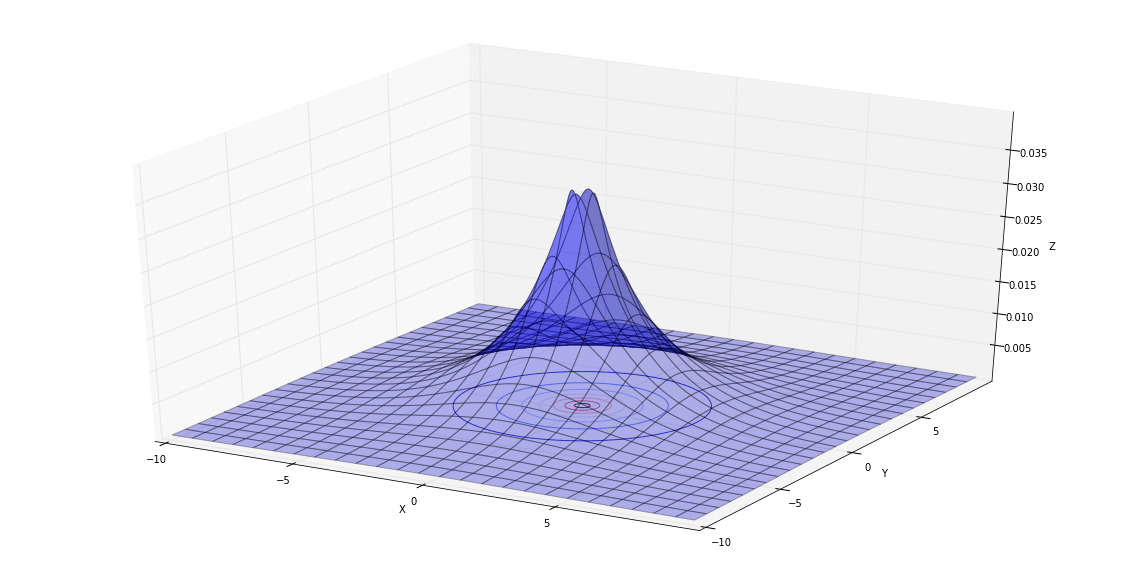
\includegraphics[scale=0.4]{kernel}
	\caption{Ejemplo de una función de kernel \(k : \calT \times \calT \to \reals\).}
\end{figure}
Podemos ver que \(\langle \phi_{1}, \phi_{2} \rangle_{\Sigma_w} = \phi_{1}^{\top} \Sigma_w \phi_{2}\) es un producto interno (con respecto a \(\Sigma_w\)) del espacio \(\calF\). Como \(\Sigma_w\) es definida positiva, se puede descomponer de forma que \(\Sigma_w = (\Sigma_w^{1/2})^{\top} \Sigma_w^{1/2}\). Por otro lado, si tomamos una descomposición en valores singulares de la matriz \(\Sigma_w = UDU^{\top}\), entonces \(\Sigma_w^{1/2} = UD^{1/2}U^{\top}\) cumple con la condición deseada. Con esto, es posible definir otra proyección
\begin{align*}
	\varphi : \calT	& \to \calF\\
	t						& \mapsto \varphi(t) = \Sigma_w^{1/2} \phi(t),
\end{align*}
de forma que el kernel \(k\) tiene forma de producto punto con respecto \(\varphi\), es decir,
\begin{align*}
	k(t_{1}, t_{2})	&= \left\langle \varphi(t_{1}), \varphi(t_{2}) \right\rangle\\
					&= \varphi(t_{1})^{\top} \varphi(t_{2})\\
					&= \phi(t_{1})^{\top} \Sigma_w \phi(t_{2}).
\end{align*}

Como la distribución posterior \(\bar{f} \mid \bar{t}, T_n, X_n\) está completamente definida en función de productos internos \(\phi(t_{1})^{\top} \Sigma_w \phi(t_{2})\), entonces es posible reemplazar dicha expresión por \(k(t_{1}, t_{2})\). Este reemplazo nos da la flexibilidad de modelar directamente el kernel \(k(t_{1}, t_{2})\), sin tener la necesidad de calcular \(\phi(t)\). Esta técnica se conoce como \emph{kernel trick}, y es útil cuando es más costoso calcular el vector de características que evaluar directamente el kernel, por ejemplo cuando la dimensión de características es infinita.

\section{Proceso Gaussiano}

Los modelos de regresión utilizando procesos gaussianos se pueden interpretar de dos formas diferentes. La primera se basa en que el kernel representa un producto interno en un espacio de gran dimensión (posiblemente infinita), y se realiza un modelo bayesiano lineal en dicho espacio. La segunda se basa en que la misma función de kernel representa la función de covarianza de un proceso estocástico, y que junto a la función de media determinan por completo el proceso gaussiano, que se puede pensar como una distribución sobre un espacio de funciones, donde la distribución predictiva se reescribe como
\begin{align*}
	p\left(\bar{f} \mid \bar{t}, T_n, \bfx_n\right)	&= \calN \left(\bar{\mu}_{\bar{f}}, \bar{\sigma}_{\bar{f}}^2\right),\\
	\bar{\mu}_{\bar{f}}								&= k(\bar{t}, T_n) \left[k(T_n, T_n) + \sigma^2 I_n\right]^{-1} \bfx_n,\\
	\bar{\sigma}_{\bar{f}}^2						&= k(\bar{t}, \bar{t}) - k(\bar{t}, T_n)^{\top} \left[k(T_n, T_n) + \sigma^2 I_n\right]^{-1} k(T_n, \bar{t}).
\end{align*}

Una de las formas más eficientes de calcular la media y la varianza posterior es utilizar la descomposición de Cholesky de la matriz \(k(T_n, T_n) + \sigma^2 I_n\), ya que los cálculos se reducen a calcular tres sistemas lineales, donde las matrices son triangulares, siendo muy eficientes y estables numéricamente.

A continuación se presenta un seudoalgoritmo para calcular la media y la esperanza posterior, además de la log-verosimilitud, utilizando la descomposición de Cholesky con el fin de ser más eficiente computacionalmente, y más estable numéricamente.

\begin{algorithm}
	\caption{Cálculo de media, varianza, y log-verosimilitud de un proceso gaussiano.}
	\begin{algorithmic}[1]
		\Require{\(T_n\) (inputs), \(\bfx_n\), (variables objetivo), \(k\) (kernel) \(\sigma^2\) (ruido) \(\bar{T}\) (\emph{inputs} de prueba).}
		\State \(L \gets\) la descomposición de Cholesky de \((k (T_n, T_n) + \sigma^2 I_n)\).
		\State \(\bfalpha \gets L^{\top} \backslash (L \backslash \bfx_n)\).
		\State \(\mean(f_{\ast}) \gets k (\bar{T}, T_n)^{\top} \bfalpha\).
		\State \(\bfv \gets L \backslash k(\bar{T}, T_n)\).
		\State \(\variance(f_{\ast}) \gets k(\bar{T}, \bar{T}) - \bfv^{\top} \bfv\).
		\State \(-\log \prob(\bfx_n \mid T_n) \gets \frac{1}{2} \bfx^{\top} \bfalpha + \sum_{i=1}^n \log(L_{ii}) + \frac{n}{2} \log(2\pi)\).
		\State \textbf{return} \(\mean(f_{\ast})\) (media), \(\variance(f_{\ast})\) (varianza), \(-\log \prob(\bfx_n \mid T_n)\) (log-verosimilitud negativa).
	\end{algorithmic}
\end{algorithm}

\begin{figure}[h]
	\centering
	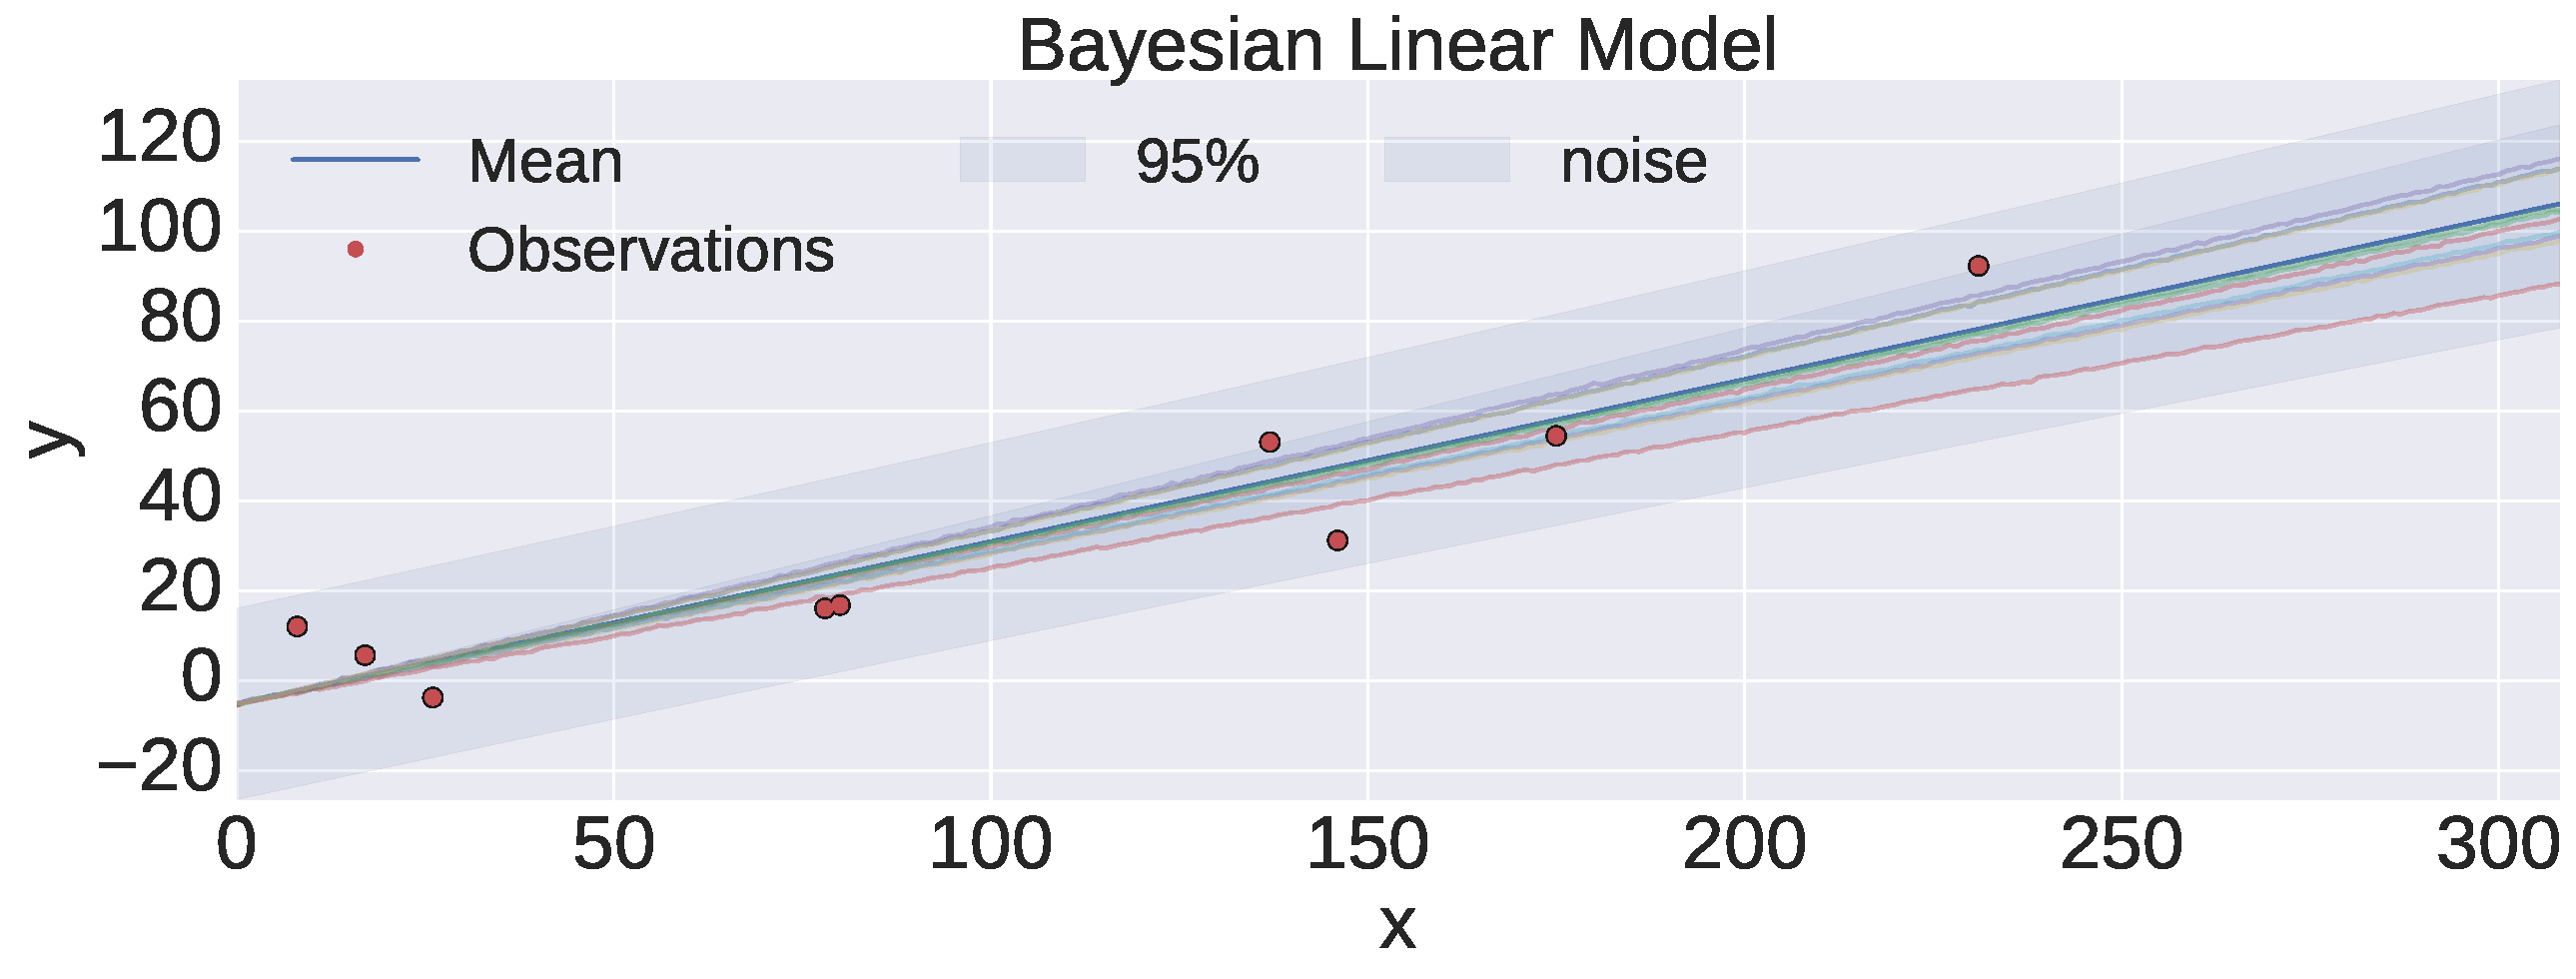
\includegraphics[width=0.49\textwidth]{bayesian_linear}
	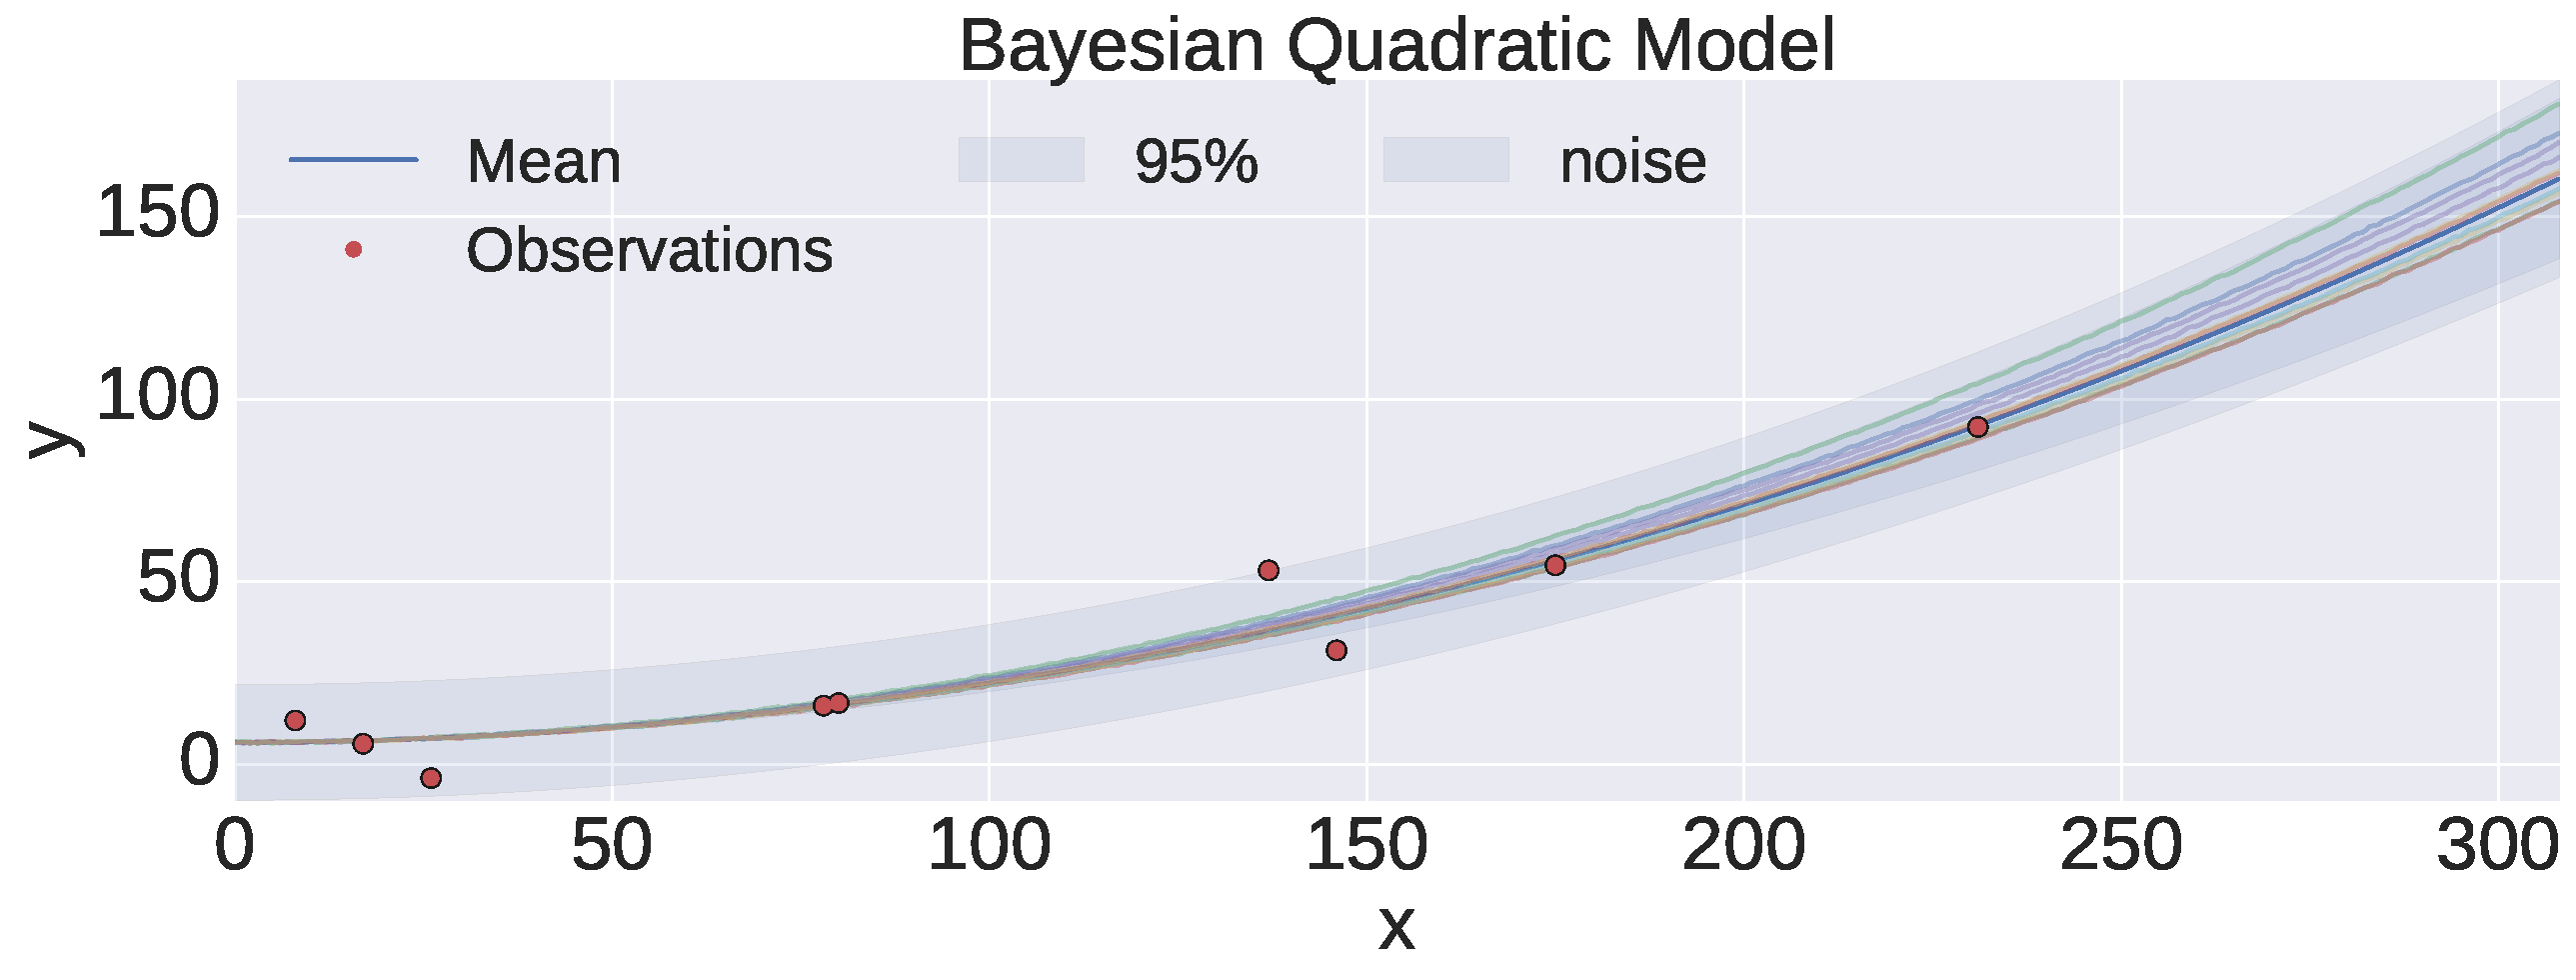
\includegraphics[width=0.49\textwidth]{bayesian_nonlinear}
	\caption{Izquierda: distribución posterior de un modelo lineal bayesiano. Derecha: distribución posterior de un modelo cuadrático bayesiano. Ambas posteriores consideran las mismas observaciones.}
	\label{fig:hierarchical_linear_quadratic}
\end{figure}

\subsection{De Redes Neuronales a Procesos Gaussianos}
\label{ssub:NN2GP}

\begin{figure}
	\centering
	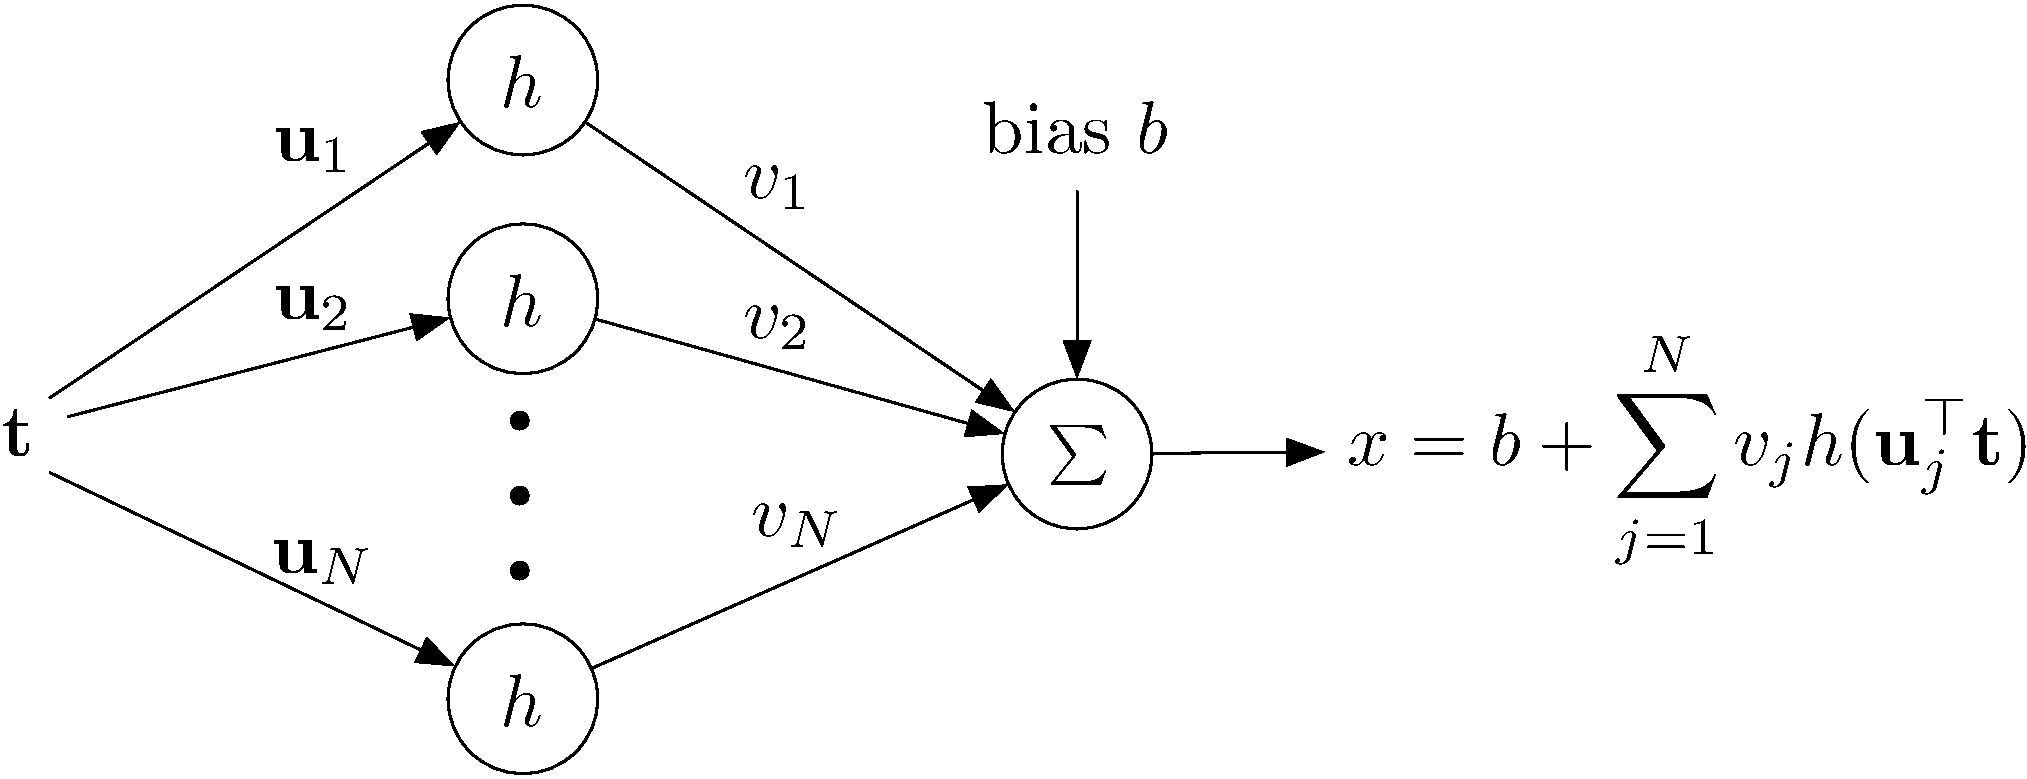
\includegraphics[width=0.5\textwidth]{nn}\\
	\caption{Red neuronal de una capa prealimentada: \(t\) es la entrada, \(x\) es la salida, \(h\) es la función de activación, \(b\) es el sesgo, \((\bfu_j)_{j=1}^N\) son los pesos de las entradas, \((\bfv_j)_{j=1}^N\) son los pesos de las salidas.}
	\label{fig:NN}
\end{figure}

Entre los practicantes de redes neuronales, se cree ampliamente que el número de neuronas debe ser determinada en base a la cantidad de datos disponible. Sin embargo, C. Williams señala en \cite{NIPS1996_1197} que esto tiene poco sentido desde un punto de vista bayesiano, en donde la complejidad del modelo se dicta por la complejidad del problema y no por la cantidad de datos disponible. En este sentido, R. Neal demostró que la salida de una red neuronal de una capa con pesos aleatorios converge a un proceso gaussiano cuando el número de neuronas tiende a infinito \cite{Neal:ARD}.

Siguiendo \cite{rasmussen06,NIPS1996_1197,Neal:ARD}, consideremos una red de \(n\) neuronas y una sola capa, como en la Figura \ref{fig:NN}. Al modelar el sesgo y los pesos como variables aleatorias independientes, las salidas \(x_1, x_2, \dotsc, x_n\) también son aleatorias para cualquier elección de entradas \(t_1, t_2, \dotsc, t_n\), con una distribución que no es necesariamente tratable debido a la función de activación no lineal \(h\). no obstante, notemos que la red en la Figura \ref{fig:NN} se define por una suma de términos i.i.d., por lo que en virtud del Teorema del Límite Central en múltiples dimensiones \cite{araujo1980central} hacer crecer el número de neuronas \(n \to \infty\) resulta en que las salidas \(x_1, x_2, \dotsc, x_n\) son conjuntamente gaussianas\footnote{La motivación de hacer crecer el número de neuronas a infinito se sigue de \cite{Hornik:1993}, que formula que la red de la Figura \ref{fig:NN} es un aproximador universal. Más aún, el TLC puede aplicarse pues como la función de activación \(h\) es acotada esto resulta en que las salidas \(x_1, x_2, \dotsc, x_n\) tienen varianza finita. Notemos que se requiere escalar la varianza de los pesos de salida proporcional a \(1/n\) para que se pueda aplicar el TLC.}. Esta construcción puede extenderse aún más al caso de un número infinito de entradas, lo que produce el proceso gaussiano \cite{rasmussen06}. En la siguiente sección profundizamos las propiedades de este modelo como un proceso estocástico.

\subsection{Distribución sobre Funciones}

Un enfoque alternativo de un proceso gaussiano consiste es describirlo como una distribución sobre funciones, donde la regresión corresponde a muestrear funciones, para luego calcular el promedio y la varianza del conjunto de funciones.
\begin{figure}[h]
	\centering
	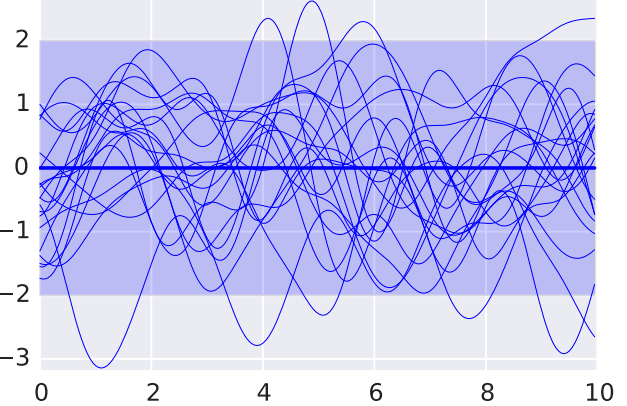
\includegraphics[scale=0.4]{gpdistribution}
	\caption{Representación gráfica de un proceso gaussiano, donde podemos distinguir su función de media, intervalos de confianza y muestras del proceso.}
\end{figure}

\begin{definition}
	Un \emph{proceso gaussiano} es una colección de variables aleatorias, donde todo subconjunto finito de ellas tiene distribución conjuntamente gaussiana.
\end{definition}

Un proceso gaussiano esta completamente especificado por su función de media \(m(t)\) y su función de covarianza \(k(t, t^{\prime})\), de forma que
\begin{align*}
	m(t)				&= \mean[f(t)],\\
	k(t, t^{\prime })	&= \mean[(f(t)-m(t))(f(t^{\prime })-m(t^{\prime}))^{\top}],
\end{align*}
y denotamos el proceso gaussiano como
\begin{equation*}
	f(t) \sim \GP(m(t), k(t, t^{\prime})).
\end{equation*}

La función de covarianza implica una distribución sobre funciones, por lo que para un conjunto de \(\no\) puntos de entrada \(\bar{T}\) podemos generar un vector aleatorio \(\bar{\bff}\) de forma que
\begin{equation*}
	\bar{\bff} \sim \calN(m(\bar{T}), k(\bar{T}, \bar{T})).
\end{equation*}

Para generar una muestra (o realización) del proceso, procedemos a calcular la descomposición de Cholesky de la matriz de covarianza \(k(\bar{T}, \bar{T})\), para luego construir una función lineal que, al evaluarla en un vector \(\bfu\) que distribuye conjuntamente como una normal unitaria, el resultado distribuye como el proceso gaussiano deseado. Esto se traduce en calcular \(L\) y simular \(\bfu\) de modo que
\begin{align*}
	k(\bar{T}, \bar{T})	&= LL^{\top},\\
	\bfu				&\sim \calN(\mathbf{0}, I_{\no}), \\
	\bar{\bff}			&= m(\bar{T}) + L\bfu.
\end{align*}

Consideremos el caso en el que las observaciones del proceso son sin ruido, es decir, \(\calD = \{(t_i, f_i)\}_{i=1}^n = \{T_n, \bff_n\}\). Sin perdida de generalidad, supongamos que nuestra función de media es
nula, es decir, \(m(t) = 0\). En efecto, en el caso general bastaría con redefinir nuestras observaciones como \(\hat{f}_i = f_i - m(t_i)\) y seguir con el análisis. Si deseamos conocer los valores \(\bar{\bff}\) que toma el proceso en \(\bar{T}\), entonces vemos que distribución conjunta de \(\bff_{n}\) y \(\bar{\bff}\) es
\begin{equation*}
	\begin{bmatrix}
		\bff_{n} \\
		\bar{\bff}
	\end{bmatrix}
	\sim \calN \left(\mathbf{0},
	\begin{bmatrix}
		k(T_n, T_n)		& k(T_n, \bar{T})\\
		k(\bar{T}, T_n)	& k(\bar{T}, \bar{T})
	\end{bmatrix}
	\right).
\end{equation*}
Luego, la distribución condicional de \(\bar{\bff}\) dados los datos \(\{T_n, \bff_{n}\}\) y el conjunto \(\bar{T}\) esta dada por
\begin{align*}
	p\left(\bar{\bff} \mid \bar{T}, T_n, \bff_{n}\right)	&= \calN\left(\bar{\mu}_{\bar{\bff}}, \bar{\sigma}_{\bar{\bff}}^2\right),\\
	\bar{\mu}_{\bar{\bff}}									&= k(\bar{T}, T_n) k(T_n, T_n)^{-1} \bff_{n},\\
	\bar{\sigma}_{\bar{\bff}}^2								&= k(\bar{T}, \bar{T}) - k(\bar{T}, T_n) k(T_n, T_n)^{-1} k(T_n, \bar{T}).
\end{align*}
La distribución condicional de cada punto \((t_i, f_i)\) dados los datos \(\{T_n, \bff_{n}\} \) está dada por \(p(f_i \mid t_i, T_n, \bff_{n}) = \calN(f_i, 0)\), lo que corresponde a una interpolación perfecta en los mismos puntos \((t_i, f_i)\), para \(i = 1, \dotsc, n\).

\subsection{Observaciones Ruidosas}

Consideremos ahora el caso más realista, en donde observamos el proceso más un ruido gaussiano, es decir \(\calD = \{(t_i,x_i)\}_{i=1}^n = \{T_n, \bfx_n\}\), donde \(x_i = f(t_i) + \varepsilon_i\) y los ruidos \(\varepsilon_i \sim \calN(0, \sigma^2)\) son independientes e idénticamente distribuidos. Siguiendo con el análisis anterior, y observando que \(\cov(x_i, y_j) = k(t_i, x_j) + \sigma^2 \delta_{ij}\), podemos ver que las probabilidades predictivas de \(\bar{\bff}\) e \(\bar{\bfx}\) están dadas por
\begin{align*}
	\begin{bmatrix}
		\bfx_n \\
		\bar{\bff}
	\end{bmatrix}
	&\sim \calN \left(\mathbf{0},
	\begin{bmatrix}
		k(T_n, T_n) + \sigma^2 I_n	& k(T_n, \bar{T})\\
		k(\bar{T}, T_n)				& k(\bar{T}, \bar{T})
	\end{bmatrix}
	\right), \\
	p\left(\bar{\bff} \mid \bar{T}, T_n, \bfx_n\right)	&= \calN\left(\bar{\mu}_{\bar{\bff}}, \bar{\sigma}_{\bar{\bff}}^2\right),\\
	p\left(\bar{\bfx} \mid \bar{T}, T_n, \bfx_n\right)	&= \calN\left(\bar{\mu}_{\bar{\bff}}, \bar{\sigma}_{\bar{\bff}}^2 + \sigma^2\right),\\
	\bar{\mu}_{\bar{\bff}}								&= \bar{\bfk}_{n}^{\top} \left[K_{n} + \sigma^2 I_n\right]^{-1}\bfx_n,\\
	\bar{\sigma}_{\bar{\bff}}^2							&= \bar{k}-\bar{\bfk}_{n}^{\top} \left[K_{n} + \sigma^2 I_n\right]^{-1} \bar{\bfk}_{n},\\
	K_{n}												&= k(T_n, T_n),\\
	\bar{\bfk}_{n}										&= k(T_n, \bar{T}),\\
	\bar{k}												&= k(\bar{T}, \bar{T}).
\end{align*}

Consideremos el caso en el que tenemos un único dato de entrada \(\bar{t}\). Podemos ver que \(\mean[\bar{f}] = \bar{\bfk}_{n} \left[K_{n} + \sigma^2 I_n\right]^{-1}\bfx_n\) es una combinación lineal de los \(n\) valores de \(\bfx_n\):
\begin{align*}
	\mean[\bar{f}]	&= \sum_{i=1}^{n} \alpha_i(\bar{t}) x_i\\
	\alpha(\bar{t})	&= \bar{\bfk}_{n}^{\top}(\bar{t}) \left[K_{n} + \sigma^2 I_n\right]^{-1},
\end{align*}
donde \(\alpha(\bar{t})\) se conoce como la \emph{función de peso} y es la representación de un suavizador linear, ya la predicción es una combinación lineal de las observaciones \(y\) suavizadas. Consideremos la descomposición en vectores propios de la matriz de covarianza:
\begin{equation*}
	K_{n} = \sum_{i=1}^{n} \lambda_i \bfu_i \bfu_i^{\top},
\end{equation*}
donde \(\lambda_i\) es su \(i\)-ésimo valor propio y \(\bfu_i\) es su correspondiente vector propio. Como \(K_{n}\) es real y simétrica semidefinida positiva, sus valores propios son reales y no negativos, y sus vectores propios son mutuamente ortogonales. Sea \(\bfx_n = \sum_{i=1}^{n} \gamma_i \bfu_i\) para coeficientes \(\gamma_i = \bfu_i^{\top} \bfx_n\). Entonces el vector de medias está dada por
\begin{align*}
	\mean[\bff_{n}]	&= K_{n} \left(K_{n} + \sigma^2 I_n\right)^{-1}\bfx_n \\
					&= \sum_{i=1}^{n} \frac{\gamma_i \lambda_i}{\lambda_i + \sigma^2} \bfu_i,
\end{align*}
donde el parámetro \(\sigma^2\) cumple el rol del nivel de suavizamiento.

A su vez, podemos ver que \(\mean[\bar{\bff}] = \bar{\bfk}_{n}^{\top} \left[K_{n} + \sigma^2 I_n\right]^{-1} \bfx_n\) es una combinación lineal de \(n\) funciones de kernels centradas en los puntos \(\bft_i\):
\begin{align*}
	\mean[\bar{\bff}]	&= \sum_{i=1}^{n} \beta_i k(t_i, \bar{t})\\
	\beta				&= \left[K_{n} + \sigma^2 I_n\right]^{-1} X_n.
\end{align*}%
Esta representación corresponde a un modelo lineal, ya que la predicción es una combinación lineal de funciones generadas por el kernel \(k(t, t^{\prime})\). Este kernel siempre existe, gracias al Teorema de Representación. Siempre y cuando \(k(t, t^{\prime})\) sea definido positivo, se dice que el kernel es una función de covarianza. En el próximo capítulo se realizará un análisis más formal de los kernel y sus espacios de funciones asociados.


\section{Entrenamiento de los Hiperparámetros}

En la sección anterior estudiamos como obtener la probabilidad predictiva, para utilizarla en la tarea de regresión. En todo momento se hizo la suposición que la función de kernel \(k(t, t^{\prime})\) estaba fija, pero en aprendizaje de máquinas deseamos encontrar el mejor modelo posible, lo que lleva a tener que encontrar el kernel y sus respectivos parámetros, que se conocen como hiperparámetros. En esta sección vamos a revisar cómo inferir los hiperparámetros para construir el modelo de regresión.

\subsection{Parametrización}
Aprender, dadas las observaciones \(\{T_n, \bfx_n\}\), es equivalente a encontrar funciones \(m\) y \(k\), usualmente parametrizadas por finitos parámetros \(\theta = (\theta_m, \theta_k) \in \reals^p\). Normalmente esto se logra vía la minimización de la la log-verosimilitud negativa, dada por
\[\ell \left(\theta\right) = \frac{n}{2}\log(2\pi) + \frac{1}{2} \left(\bfx_n - \mu \right)^{\top} K^{-1} \left(\bfx_n-\mu \right) + \frac{1}{2} \log \lvert K\rvert,\]
donde \(\mu\) y \(K\) son la media y la covarianza de \(\bfx_n\) dados los parámetros \(\theta = (\theta_m, \theta_k)\) y los inputs \(T_n\). Los métodos de optimización más usados son los basados en el gradiente, como el método BFGS de quasi-Newton, o métodos libre de derivadas como el método de Powell. En la Figura \ref{fig:gp_sunspots_example} mostramos un GP con un kernel \(\mathrm{SE}\) y con observaciones de actividad de manchas solares. El gráfico de la izquierda muestra el proceso con los hiperparámetros por defecto, mientras que el de la derecha tiene los hiperparámetros entrenados vía la log-verosimilitud negativa. En el segundo caso, la media está más cerca de la señar real (oculta), y el intervalo de confianza es más delgado, así que la predicción tiene menos incertidumbre.

Para la log-verosimilitud negativa donde la función de media es nula, la \(j\)-ésima componente del gradiente corresponde a la derivada parcial con respecto al parámetro \(\theta_j\) la cual se puede calcular como
\begin{align*}
	\pdv{\ell}{\theta_j}	&= \frac{1}{2}\bfx_n^{\top} K^{-1} \pdv{K}{\theta_j} K^{-1} \bfx_n + \frac{1}{2} \tr \left\vert K^{-1} \pdv{K}{\theta_j} \right\vert \\
							&= -\frac{1}{2} \tr\left(\left(K^{-1} \bfx_n \bfx_n^{\top} K^{-1} - K^{-1}\right) \pdv{K}{\theta_j}\right),
\end{align*}
donde \(\tr(A)\) denota la traza de la matriz \(A\).

La complejidad de computar la verosimilitud está dada por la inversión de la matriz \(K\), por lo que los métodos estándares de inversión de matrices simétricas definidas positivas de tamaño \(n \times n\) requieren tiempo \(O(n^{3})\). Una vez que la inversa está calculada, calcular la derivada requiere tiempo \(O(n^2)\) por cada hiperparámetro

\subsection{Seudoverosimilitud}

Los métodos de validación cruzada (\emph{cross-validation} en inglés) son métodos para seleccionar modelos. La idea más simple es la de dividir el conjunto de datos en dos conjuntos disjuntos: un conjunto de entrenamiento (\emph{training set} en inglés), el cual se utiliza para entrenar el modelo, y un conjunto de validación (\emph{validation set} en inglés), que se usa para medir el desempeño (o error) del modelo. Este método se conoce en inglés como \emph{holdout cross-validation}, y tiene el problema que si el conjunto de validación es pequeño, entonces la estimación del error tiene gran varianza.

Una alternativa es el método de validación cruzada en \(k\) iteraciones (\emph{k-fold cross-validation} en inglés), en done se divide el conjunto de datos en \(k\) conjuntos disjuntos de igual tamaño. Luego, cada conjunto es utilizado para validar y los otros \(k-1\) conjuntos son utilizados para entrenar, por lo que se realizan \(k\) entrenamientos y \(k\) estimaciones del desempeño, disminuyendo así la varianza de la estimación del error al tomar promedio. Un caso extremo es considerar \(k=n\). Esta validación cruzada dejando uno afuera (\emph{leave-one-out cross-validation} en inglés, y denotado denotado LOO más abajo) es utilizada sólo en casos particulares, por su alto costo computacional. En este caso, la log-probabilidad predictiva cuando se deja afuera el caso \(i\) es
\begin{align*}
	\log p(x_i \mid T_n, \bfx_{-i}, \theta)	&= -\frac{1}{2} \log (\sigma_i^2) - \frac{(x_i - \mu_i)^2}{2\sigma_i^2} - \frac{1}{2} \log(2\pi), \\
	\mu_i										&= K(t_i, T_{-i}) \left[K(T_{-i}, T_{-i}) + \sigma^2 I\right]^{-1} \bfx_{-i} \\
												&= x_i - \frac{[K^{-1} \bfx_n]_i}{[K^{-1}]_{ii}},\\
	\sigma_i^2								&= K(t_i, t_i) - K(t_i, T_{-i}) \left[K(T_{-i}, T_{-i}) + \sigma^2 I\right]^{-1} K(T_{-i}, t_i) \\
												&= \frac{1}{[K^{-1}]_{ii}} \\
	\log p(x_i \mid T_n, \bfx_{-i}, \theta)	&= \frac{1}{2}\log [K^{-1}]_{ii} - \frac{[K^{-1} \bfx_n]_i^2}{2 [K^{-1}]_{ii}} - \frac{1}{2} \log(2\pi),
\end{align*}
donde \(K = k(T_n, T_n)\), \(\bfx_{-i} = \bfx_n \setminus \{x_i\}\) y \(~T_{-i} = T_n \setminus \{t_i\}\). Luego, la log-probabilidad predictiva de LOO es
\begin{equation*}
	L_{LOO}(T_n, \bfx_n, \theta) = \sum_{i=1}^{n} \log p(x_i \mid T_n, \bfx_{-i}, \theta),
\end{equation*}
la cual se conoce como la seudo-log-verosimilitud (\emph{pseudo-log-likelihood} en inglés). Dada la inversa de \(K\), calcular \(L_{LOO}\) requiere tiempo \(O(n^2)\), y esta puede ser utilizada como estimador a optimizar con respecto a los hiperparámetros, quedando de la forma
\begin{equation*}
	L_{LOO}(T_n, \bfx_n, \theta) = -\frac{n}{2}\log(2\pi) + \frac{1}{2} \sum_{i=1}^{n} \left(\log [K^{-1}]_{ii} - \frac{[K^{-1} \bfx]_i^2}{[K^{-1}]_{ii}}\right).
\end{equation*}

Para calcular las derivadas parciales de \(L_{LOO}\) con respecto los hiperparámetros, veamos las derivas de las medias y las varianzas marginales.
\begin{align*}
	\pdv{\mu_i}{\theta_j}		&= -\pdv{\theta_j} \frac{\left[K^{-1} \bfx_n \right]_i}{[K^{-1}]_{ii}} \\
								&= \frac{\left[K^{-1} \pdv{K}{\theta_j} K^{-1} \bfx_{n}\right]_i [K^{-1}]_{ii} - \left[K^{-1} \bfx_n\right]_{ii} \left[K^{-1} \pdv{K}{\theta_j} K^{-1}\right]_{ii}}{[K^{-1}]_{ii}^2} \\
								&= \frac{\left[K^{-1} \pdv{K}{\theta_j} K^{-1} \bfx_{n}\right]_i}{[K^{-1}]_{ii}} - \frac{\left[K^{-1} \bfx_{n}\right]_{ii} \left[K^{-1} \pdv{K}{\theta_j} K^{-1}\right]_{ii}}{[K^{-1}]_{ii}^2}\\
	\pdv{\sigma_i^2}{\theta_j}	&= -\pdv{\theta_j} \frac{1}{[K^{-1}]_{ii}} \\
								&= \frac{\left[K^{-1} \pdv{K}{\theta_j} K^{-1}\right]_{ii}}{[K^{-1}]_{ii}^2}.
\end{align*}
Las derivadas con respecto a la media y la varianza de la log-probabilidad predictiva del \(i\)-ésimo término son
\begin{align*}
	\pdv{\mu_i} \log p(x_i \mid T_n, \bfx_{-i}, \theta)		&= \frac{x_i - \mu_i}{\sigma_i^2} = \left[K^{-1} \bfx_n \right]_i \\
	\pdv{\sigma_i^2}\log p(x_i \mid T_n, \bfx_{-i}, \theta)	&= \frac{(x_i - \mu_i)^2 - \sigma_i^2}{2 \sigma_i^4} = \frac{1}{2} \left[\left[K^{-1} \bfx_n\right]_i^2 - [K^{-1}]_{ii}\right].
\end{align*}
Luego, la derivada parcial de \(L_{LOO}\) con respecto al hiperparámetro \(\theta_j\) es
\begin{align*}
	\pdv{L_{\mathrm{LOO}}}{\theta_j}=	& \sum_{i=1}^{n} \pdv{\mu_i}{\theta_j} \pdv{\mu_i} \log p(x_i \mid T_n, \bfx_{-i}, \theta) + \pdv{\sigma_i^2}{\theta_j} \pdv{\sigma_i^2} \log p(x_i \mid T_n, \bfx_{-i}, \theta) \\
										=& \sum_{i=1}^{n} \frac{\left[K^{-1} \pdv{K}{\theta_j} K^{-1} \bfx_n \right]_i}{[K^{-1}]_{ii}} \left[K^{-1} \bfx_n\right]_i - \frac{\left[K^{-1} \bfx_n\right]_i \left[K^{-1} \pdv{K}{\theta_j} K^{-1}\right]_{ii}}{[K^{-1}]_{ii}^2} \left[K^{-1} \bfx_n\right]_i \\
										&+ \frac{\left[K^{-1} \pdv{K}{\theta_j} K^{-1}\right]_{ii} \left[\left[K^{-1} \bfx_n\right]_i^2 - \left[K^{-1}\right]_{ii}\right]}{2[K^{-1}]_{ii}^2} \\
										=& \sum_{i=1}^{n} \frac{\left[K^{-1} \bfx_n\right]_i}{\left[K^{-1}\right]_{ii}} \left[\left[K^{-1} \pdv{K}{\theta_j} K^{-1} \bfx_n\right]_i - \frac{[K^{-1}]_{ii} + \left[K^{-1} \bfx_n\right]_i^2}{2 \left[K^{-1} \bfx_n\right]_i[K^{-1}]_{ii}} \left[K^{-1} \pdv{K}{\theta_j} K^{-1}\right]_{ii}\right]
\end{align*}
Dada la inversa de \(K^{-1}\), la complejidad computacional de calcular una derivada parcial es de \(O(n^{3})\) por cada hiperparámetro, dominada por el término \(K^{-1} \pdv{K}{\theta_j} K^{-1}\). Mientras la función de verosimilitud marginal es la probabilidad de las observaciones dado el modelo, la función de seudoverosimilud es un estimador de la probabilidad predictiva del modelo.

\subsection{Selección de Variables}

Al momento de escoger un modelo, existe una gran variedad de familias de kernels (que se estudiarán en el próximo capítulo), donde cada una dispone de una cierta cantidad de hiperparámetros, los cuales deben ser entrenados (como vimos en las secciones anteriores), y esto depende fuertemente de la cantidad de variables que consideremos en el espacio de entrada, es decir de la dimensión \(d\) del espacio \(\calT\). El concepto de selección de modelo (\emph{model selection} en inglés) se refiere a la tarea general de escoger la familia de kernels, las variables de entrada y los hiperparámetros de un modelo.

En el caso que la dimensión \(d\) del espacio de entrada \(\calT\) sea mayor a uno, entonces los kernels deben permitir evaluar en todas las dimensiones. Puede darse el caso de que alguna de las dimensiones no afecte en la covarianza, ya sea porque la salida es independiente de esa dimensión o porque es redundante dada las demás dimensiones. En estos casos, reducir la dimensión del espacio \(\calT\) es deseable con el fin de bajar la complejidad del modelo. La opción más común es utilizar análisis de componentes principales (abreviado PCA pro sus siglas en inglés) sobre \(T_n\), pero este enfoque no es el más correcto, ya que no utiliza la información de \(\bfx_n\).

Consideremos el kernel \emph{square exponential}, dado por
\begin{equation*}
	k_{\mathrm{SE}} (t, \bar{t}) = h^2 \exp\left(-w^2 \left\Vert t - \bar{t} \right\Vert^2\right) = h^2 \exp\left(-w^2 \sum_{j=1}^{d} \left(t_j - \bar{t}_j\right)^2\right),
\end{equation*}
donde \(h\) y \(w\) son sus hiperparámetros. Se dice que este kernel es isotrópico, ya que todas las dimensiones de entrada son uniformes, supuesto que en muchos casos no es válido. La versión anisotrópica, conocida como \emph{automatic relevance determination} y denotada ARD, dada por
\begin{equation*}
	k(t, \bar{t}) = h^2 \exp\left(\sum_{j=1}^{d} w_d^2 (t_j - \bar{t}_j)^2\right),
\end{equation*}
tiene un hiperparámetro \(w_d^2\) por cada dimensión. Si \(w_d^2\) es muy pequeño o igual a \(0\), entonces se interpreta que la variable \(x_d\) no agrega información en la covarianza, por lo que son poco relevantes. Esto nos permite utilizar este kernel para eliminar variables poco relevantes. Una versión más sofisticada es el kernel de la forma
\begin{equation*}
	k(t, \bar{t}) = h^2 \exp\left(-\frac{1}{2} (t - \bar{t})^{\top} \left(\Lambda \Lambda^{\top} + \diag(w^2)\right) (t - \bar{t}) \right),
\end{equation*}
llamado la distancia del análisis de factor (\emph{factor analysis distance} en inglés), el cual generaliza el ARD con \(w = (w_1, \dotsc, w_D)\) y una matriz \(\Lambda\) de dimensión \(d \times k\), con \(k < d\). Además de determinar las relevancias individuales, las \(k\) columnas de \(\Lambda\) pueden identificar las direcciones que son más relevantes para explicar la varianza. Este kernel hace la analogía con el análisis factorial. Otro enfoque es considerar el kernel
\begin{equation*}
	k(t, \bar{t}) = \sum_{j=1}^{N} \frac{\phi_j(t) \phi_j(\bar{t})}{\alpha_j},
\end{equation*}
llamado máquina de relevancia vectorial (\emph{relevance vector machine} en inglés), donde \(\{\phi_j\}_{j=1}^{N}\) es una base de funciones. Este kernel permite reconocer las componentes \(\phi_j\) relevantes para explicar la covarianza, por lo que se pueden escoger las funciones base con diferentes conjuntos de variables de entrada, para así reconocer cuales son los conjuntos de variables más relevantes. Esta idea se puede extender con
\[k (t, \bar{t}) = \sum_{j=1}^{N} \frac{k_j(t, \bar{t})}{\alpha_j}.\]
	%!TEX root = main.tex

\chapter{Funciones de Kernel}


\begin{chapquote}{Gonzalo Ríos, 2023}
	``Aquí falta una cita.''
\end{chapquote}

Como vimos en el capítulo anterior, la función de covarianza es el elemento crucial en un GP, ya que contiene la información \emph{a priori} del espacio de funciones del cual queremos estimar. Las funciones de covarianza se modelan usualmente con funciones de \emph{kernels}, y se tiene en cuenta el siguiente supuesto de similitud: los puntos del espacio de \emph{inputs} que están más cerca entre sí tienen valores más correlacionados en el espacio de estados. En este capitulo vamos a definir formalmente que es un kernel y veremos las familias de kernels más utilizados y sus propiedades generales.

\comment{parrafo: introducción y motivación del capitulo}

\comment{parrafo: resumen del capitulo}

\section{Analisis Funcional}

\comment{en particular en este capitulo trataria de incluir intuición, ya que se empieza a poner medio oscuro. La idea es no perder al lector}

En general, vamos a llamarle kernel a toda función de la forma \(k : \calT \times \calT \to \reals\). El siguiente gráfico nos muestra la forma de uno de los kernels más utilizados, el kernel gaussiano.

La familia de kernels que nos va a interesar es la de kernels simétricos definidos positivos (que definen funciones de covarianza), concepto que coincide con generalización de las matrices definidas positivas. A continuación, aplicaremos algunos resultados clásicos de análisis funcional a las funciones de kernels, con el fin de poder caracterizar algunas propiedades de las funciones que generan.

\subsection{Funciones de Covarianza}


Las propiedades que deseamos estudiar están relacionadas con los kernels que son definidos positivos. Para poder definir esta propiedad sobre los kernels, veamos primero la definición para matrices.

\begin{definition}
	Una matriz con coeficientes reales \(K\) de \(n \times n\) se dice que es semidefinida positiva (denotado SDP) si para todo vector \(\bfv \in \reals^n\) se cumple que \(Q(\bfv) \coloneqq \bfv^{\top} K \bfv \geq 0\). Si además se cumple que \(Q(\bfv) = 0 \iff \bfv = \mathbf{0}\), entonces se dice que la matriz \(K\) es definida positiva (denotado DP).
\end{definition}


Análogamente, podemos extender la definición de semidefinido positivo a los kernels de forma natural.

\begin{definition}
	Se dice que un kernel \(k : \calT \times \calT \to \reals\) es semidefinido positivo si para toda función \(f \in L^{2}(\calT, \mu) \) (el espacio de funciones de \(\calT\) a \(\complex\) que son cuadrado-integrables con respecto la medida \(\mu\)) se cumple que
	\begin{equation*}
		\int_{\calT} \int_{\calT} k(t, \bar{t}) f(t) f(\bar{t}) \dd{\mu(t)} \dd{\mu(\bar{t})} \geq 0.
	\end{equation*}
\end{definition}

Una matriz de Gram que se corresponde con una función de kernel general no es necesariamente SDP, pero una matriz de Gram de una función de covarianza siempre es SDP. Dada una función de covarianza, diremos que toda matriz de Gram es una matriz de covarianza. El siguiente resultado caracteriza la SDP de un kernel con la de sus matrices de Gram.

\begin{proposition}
	Un kernel \(k\) es semidefinido positivo si y sólo si toda matriz de Gram \(K\) generada con \(k\) es semidefinida positiva. En ese caso, se dice que \(k\) es una función de covarianza.
\end{proposition}


\subsection{Valores Propios y Funciones Propias}
Uno de los análisis más clásicos es el de valores propios. Como estamos hablando de un kernel, cada valor propio está asociado a lo que se conoce como una función propia (\emph{eigenfunction} en inglés\footnote{El prefijo \emph{eigen} viene del alemán, y significa «propio», «característico». En muchas lenguas el prefijo no se traduce, pero en español es usual traducirlo o usar el prefijo \emph{auto-}.}), que gracias al teorema de Mercer nos permite descomponer el kernel, y así caracterizar la suavidad de las funciones generadas.

Un resultado muy conocido es la caracterización de los valores propios de matrices SDP.

\begin{proposition}
	Una matriz simétrica es semidefinida positiva si y solo si todos sus valores propios son no negativos.
\end{proposition}

Es fácil ver la implicancia de que si \(K\) tiene un valor propio \(\lambda_{i}\) negativo entonces la matriz no es SDP. En efecto, basta con tomar el vector propio ortonormal \(\bfu_{i}\) asociado a ese \(i\)-ésimo valor propio, y evaluando en la ecuación anterior se tiene que
\begin{equation*}
\bfv_{i}^{\top} K\bfv_{i} = \bfu_{i}^{\top} \lambda_{i} \bfu_{i} = \lambda_{i} < 0.
\end{equation*}%
La otra implicancia se basa en que todo vector es combinación lineal de los vectores propios de \(K\), por lo que
\begin{align*}
\bfv				&= \sum_{i=1}^{n} a_{i} \bfu_{i} \\
\bfv^{\top}K\bfv	&= \sum_{i=1}^{n} \sum_{j=1}^{n} a_{i} a_{j} \bfu_{i}^{\top} K \bfu_{j} \\
&= \sum_{i=1}^{n} \sum_{j=1}^{n} a_{i}a_{j} \lambda_j \bfu_{i}^{\top} \bfu_{j}\\
&= \sum_{i=1}^{n} a_{i}^{2} \lambda_{i},
\end{align*}
por lo que es no negativo para todo \(\bfv\) no nulo si todos los valores propios son positivos.

A continuación tenemos la definición de funciones y valores propios de un kernel.


\begin{definition}
	Dado un kernel de covarianza \(k(t, \bar{t})\), entonces toda función \(\phi\) que cumple la ecuación integral
	\begin{equation*}
		\int k(t, \bar{t}) \phi(t) \dd{\mu} \left(t\right) = \lambda \phi(\bar{t})
	\end{equation*}
	se dice que es una función propia de \(k\), donde \(\lambda\) es su valor propio con respecto a la medida \(\mu\).
\end{definition}

\begin{proposition}
	Existen infinitas funciones propias asociadas a un kernel \(k\), y pueden ser escogidas de forma ortonormal, es decir,
	\[\int \phi_{i} (t) \phi_{j}(t) \dd{\mu(t)} = \delta_{ij}.\]
\end{proposition}

El siguiente resultado es el famoso teorema de Mercer, el cual da una representación del kernel como la suma convergente de producto de funciones propias.

\begin{theorem}[Mercer]
	Sean \((\calT, \mu)\) un espacio de medida finita, \(k \in L^{\infty}(\calT^{2}, \mu^{2})\) un kernel semidefinido positivo, y \(T_{k} : L^{2}(\calT, \mu) \to L^{2}(\calT, \mu)\) el operador lineal asociado a \(k\) dado por
	\begin{equation*}
		[T_{k}(f)](s) = \int k(s, t) f(t) \dd{\mu(t)}.
	\end{equation*}
	Sean \(\phi_{i} \in L^{2}(\calT, \mu)\) las funciones propias ortonormales asociadas a \(T_{k}\) con valores propios \(\lambda_{i}\) (que existen pues \(T_k\) es un operador lineal). Entonces:
	
	\begin{enumerate}
		\item La secuencia de valores propios \((\lambda_{i})_{i \in \naturals}\) están en \(\ell^{1}\), es decir
		\[\sum_{i=1}^{\infty} \left\vert \lambda_{i} \right\vert < \infty.\]
		\item El kernel tiene la representación
		\[ k(t, \bar{t}) = \sum_{i=1}^{\infty} \lambda_{i} \phi_{i}(t) \phi_{i}^{\ast}(\bar{t}),\]
		en casi todos los puntos \(\mu^{2}\)-c.t.p., donde la serie converge uniformemente \(\mu^{2}\)-c.t.p.
	\end{enumerate}
\end{theorem}

La tasa de decaimiento de los valores propios entrega una información importante sobre la suavidad del kernel. Procesos más suaves tienden a tener valores propios \(\lambda_{i}\) bajos para las altas frecuencias \(i\), es decir, a mayor tasa de decaimiento, más suave es el proceso.


\begin{definition}
	Un kernel se dice degenerado si sólo tiene una cantidad finita de valores propios distintos a cero. También se dice que el kernel es de rango finito.
\end{definition}


\subsection{Espacios de Hilbert de Kernels reproducibles}

Otra forma de analizar un kernel es analizando el espacio de funciones que genera, e incluso podemos construir un espacio de Hilbert asociado a un kernel definido positivo \cite{steinwart2006explicit}. Podemos tanto expresar el producto interno de dicho espacio como caracterizar las funciones del espacio en función del kernel. Los resultados son los siguientes.

\begin{definition}
	Sea \(\calH\) un espacio de Hilbert de funciones definidas sobre un conjunto \(\calT\) a valores reales, dotado de un producto interno \(\langle \cdot, \cdot \rangle_{\calH}\). Se dice que \(\calH\) es un espacio de Hilbert con kernel de reproducción (denotado RKHS por sus siglas en inglés, \emph{reproducing kernel Hilbert space}) si existe un kernel semidefinido positivo \(k : \calT \times \calT \to \reals\) que cumpla:
	\begin{enumerate}
		\item Para todo \(\bar{t} \in \calT\), la función \(k_{\bar{t}}\) dada por  \(k_{\bar{t}}(t) = k(t, \bar{t})\) pertenece a \(\calH\).
		\item \(k\) tiene la propiedad de reproducción, es decir, \(\langle f, k_{\bar{t}} \rangle_{\calH} = f(\bar{t})\).
	\end{enumerate}
\end{definition}

La definición anterior caracteriza un kernel con respecto al espacio de funciones que genera (o reproduce), donde las funciones elementales de dicho espacio son las proyecciones de \(k\) en una de sus variables, es decir, \(\{ k_{\bar{t}}(t) = k(t, \bar{t})\}_{\bar{t} \in \calT}\). La propiedad de reproducción asocia al kernel con el funcional lineal de evaluación
\begin{align*}
	L_{\bar{t}}(f)	&= \int k(\bar{t}, t) f(t) \dd{\mu(t)} \\
					&= \langle k_{\bar{t}}, f\rangle_{\calH} \\
					&= f(\bar{t}).
\end{align*}
Este funcional se dice acotado si su norma es acotada,
\begin{align*}
	\Vert L_{\bar{t}} \Vert	&= \sup_{f \in \calH} \frac{\Vert L_{\bar{t}}(f) \Vert}{\Vert f \Vert } \\
							&= \sup_{\Vert f \Vert_{\calH} = 1} \Vert f(\bar{t}) \Vert\\
							&< \infty,
\end{align*}
es decir, que toda función generada por el espacio es acotada en \(\bar{t}\), lo cual es equivalente a que el kernel \(k\) sea acotado en \(\bar{t}\):
\begin{equation*}
	\Vert k_{\bar{t}}\Vert_{\calH} < \infty.
\end{equation*}
Como las funciones \(k_{\bar{t}}\) pertenecen al espacio \(\calH\), entonces su norma es finita, por lo que el funcional de evaluación en \(\bar{t}\) es continuo. Veamos a continuación el importante teorema de representación de Riesz \cite{friedman1982foundations}.

\begin{theorem}[Representación de Riesz]
	Para todo funcional lineal acotado \(L\) definido sobre un espacio de Hilbert \(\calH\) existe un único elemento \(k \in \calH\) tal que
	\begin{equation*}
		L(f) = \langle f, k\rangle_{\calH}
	\end{equation*}
\end{theorem}

\begin{corollary}[Propiedad Reproductiva] Para todo \(f \in \calH\) existe un único elemento \(k_{\bar{t}} \in \calH\) tal que el mapeo de evaluación cumple
	\begin{equation*}
		L_{\bar{t}}(f) = f(\bar{t}) = \langle f, k_{\bar{t}}\rangle_{\calH}.
	\end{equation*}
\end{corollary}

La propiedad reproductiva nos permite asociar el kernel \(k\) con la evaluación de forma que se cumplen las siguientes propiedades en:
\begin{itemize}
	\item \(f(\bar{t}) = \langle f, k_{\bar{t}}\rangle_{\calH} = \int k(\bar{t}, t) f(t) \dd{\mu(t)}\).
	\item \(k(t, \bar{t}) = \langle k_{x}, k_{\bar{t}} \rangle_{\calH}\).
	\item \(k(\bar{t}, \bar{t}) = \langle k_{\bar{t}}, k_{\bar{t}}\rangle_{\calH} = \Vert k_{\bar{t}} \Vert_{\calH}^{2}\).
	\item \(k_{\bar{t}} = 0 \iff \ f(\bar{t}) = 0\) para toda función \(f \in \calH\).
	\item \(k_{\bar{t}}(t) = \int k(t, z) k_{\bar{t}}(z) \dd{\mu(z)} = \int k(t, z) k(\bar{t}, z) \dd{\mu(z)} = k_{t}(\bar{t}) \).
\end{itemize}

Ahora nos gustaría caracterizar el tipo de espacios de funciones que son RKHS. Para empezar, no todo espacio de Hilbert es RKHS.
\begin{proposition}
	El espacio de Hilbert \(L^{2}\) con el producto interno \(\langle f, g\rangle_{L^{2}} = \int f(t) g(t) \dd{x}\) no es RKHS.
\end{proposition}

En efecto, basta con encontrar una función que en algún \(\bar{t}\) no sea finita, pero sí sea cuadrado-integrable. Consideremos la función \( f(t) = \sqrt{x^\alpha} \). Entonces,
\begin{align*}
	\langle f, f \rangle_{L^{2}}	&= \int_{0}^{1} x^\alpha \dd{x} \\
									&= \frac{1}{\alpha + 1},
\end{align*}
y la última igualdad solo se cumple si \(\alpha + 1 > 0\). Tomando \(\alpha =-\frac{1}{2}\) tenemos que
\[f(t) = t^{-\frac{1}{4}} = \frac{1}{(t)^{\frac{1}{4}}},\]
que no es acotada en \(\bar{t} = 0\) y el resultado se concluye.

El siguiente resultado \cite{aronszajn1950theory} nos entrega la existencia y unicidad de la correspondencia entre el kernel \(k\) y espacio RKHS \(\calH\).
\begin{theorem}[Moore-Aronszajn] Sea \(\calT\) un conjunto y sea \(k\) un kernel definido positivo en \(\calT \times \calT\). Entonces existe un único RKHS asociado a \(k\), es decir, un espacio de Hilbert \(\calH\) para el cual \(k\) es kernel de reproducción. Además, cada RKHS tiene un único kernel definido positivo asociado.
\end{theorem}

Ahora que sabemos que la correspondencia es única entre un kernel definido positivo y un RKHS, caractericemos el espacio \(\calH\) en función de la base ortogonal que conforman las funciones propias del kernel \(k\). El caso degenerado tiene representación finita.

\begin{proposition}
	Sea \(\calH\) el espacio de Hilbert de combinaciones lineales de las funciones propias ortogonales \((\phi_{i})_{i=1}^{N}\) de un kernel \(k\) con respecto a una medida \(\mu\), compuesto por funciones de la forma
	\[f(t) = \sum_{i=1}^{N} f_{i} \phi_{i}(t),\]
	que cumplan que
	\[\sum_{i=1}^{N} \frac{f_{i}^{2}}{\lambda_{i}} < \infty.\]
	Si dotamos a \(\calH\) con el producto interno
	\[\langle f,g \rangle_{\calH} = \sum_{i=1}^{N} \frac{f_{i} g_{i}}{\lambda_{i}},\]
	donde \(\lambda_{i}\) es el valor propio asociado a \(\phi_{i}\), entonces \(\calH\) es el RKHS asociado a \(k\).
\end{proposition}

Para el caso no degenerado, las funciones se construyen a partir de combinaciones de las funciones elementales \(k_{\bar{t}}\), para luego tomar la adherencia del espacio de Hilbert (por completitud del espacio).
\begin{proposition}[Representante]
	Dado un kernel \(k\) sobre \(\calT\), consideremos el espacio de funciones
	\[ \calH = \left\{ f(t) = \sum_{i=1}^{n_{f}} f_{i} k(t, t_{i}) : n_{f} \in \naturals, t_{i}\in \calT, f_{i} \in \reals \right\},\]
	con el producto interno
	\[\langle f, g\rangle_{\calH} = \sum_{i=1}^{n_{f}} \sum_{j=1}^{n_{g}} f_{i}g_{j} k(t_{i}, t_{j}).\]
	Entonces \(\calH\) es el RKHS asociado a \(k\).
\end{proposition}

Es directo que \(\calH\) es RKHS, ya que el kernel \(k\) cumple las propiedades de reproducción:
\begin{align*}
	f(t)									&= k_{\bar{t}} (t) \in \calH \text{, con } n_{f} = 1, t_{1} = \bar{t}, \text{ y } f_{i}=1, \\
	\langle f, k_{\bar{t}} \rangle_{\calH}	&= \sum_{i=1}^{n_{f}} f_{i} k(\bar{t}, t_{i}) = f(\bar{t}),
\end{align*}%
y por unicidad se tiene que \(k\) es su kernel asociado. Esta última representación corresponde a un número (posiblemente infinito) de funciones bases, correspondientes a proyecciones del kernel. Esta representación se mantiene incluso al considerar un factor de regulación, que nos permitirá imponer ciertas condiciones sobre \(f(t)\).

\subsection{Regularización}

Bajo en enfoque bayesiano, nuestro supuesto sobre la función a modelar esta caracterizado por una probabilidad \emph{a priori} del espacio de funciones \cite{rasmussen06}, pero también existe el enfoque de \emph{regularización}, donde nuestros supuestos son sobre la suavidad de la función. Consideremos el funcional
\begin{equation*}
	J[f] = Q(\bfx_{n}, \bff_{n}) +\frac{\lambda}{2} \Vert f \Vert_{RKHS}^{2},
\end{equation*}
donde \(\bfx_{n}\) es el vector de observaciones y \(\bff_{n}\) es el vector de estimaciones en los puntos \(X_{n}\). El primer término evalúa la calidad del ajuste, por lo que \(Q\) puede representar el error cuadrático  \(\Vert \bfx_{n} - \bff_{n}\Vert^{2}\) o la log-verosimilitud negativa NLL. El segundo término, llamado regularizador, evalúa el supuesto de suavidad de \(f\) a través de la norma \(\Vert f\Vert_{RKHS}\) correspondiente a un kernel \(k\), además de tener un parámetro de escala \(\lambda\) que equilibra ambos términos.

Consideremos el funcional de la forma \cite{kimeldorf1971some}
\begin{equation*}
	J[f] = \frac{1}{2} \Vert f \Vert_{RKHS}^{2} + \frac{1}{2 \sigma^2} \sum_{i=1}^{n} (x_{i} - f(t_{i}))^{2}.
\end{equation*}%
Por el teorema de representación en espacios RKHS, la función \(f\) que minimiza \(J\) tiene la forma \(f(t) = \sum\nolimits_{i=1}^{n} \alpha _{i} k(t, t_{i})\), y como \(\langle k(\cdot, t_{i}), k(\cdot, t_{j})\rangle_{\calH} = k(t_{i}, t_{j})\) entonces
\begin{align*}
	J[f]	&= \hat{J}[\bfalpha]\\
			&= \frac{1}{2} \bfalpha^{\top }K_{n} \bfalpha + \frac{1}{2\sigma^2} \vert \bfx - K_{n}\bfalpha \vert^{2} \\
			&= \frac{1}{2} \bfalpha^{\top} \left(K_{n} + \frac{1}{\sigma^2} K_{n}^{2}\right) \bfalpha - \frac{1}{2\sigma^2} \bfx^{\top} K_{n} \bfalpha + \frac{1}{2 \sigma^2} \bfx^{\top} \bfx,
\end{align*}
donde \(K_{n} = k(T_{n}, T_{n})\). Minimizando \(\hat{J}[\bfalpha]\) con respecto a \(\bfalpha\), entonces se tiene que
\begin{align*}
	\dv{\hat{J}[\bfalpha]}{\bfalpha} = 0	& \implies \bfalpha^{\top} \left(K_{n} + \frac{1}{\sigma^2} K_{n}^{2}\right) - \frac{1}{2\sigma^2} \bfx^{\top}K_{n} = 0 \\
											& \implies \hat{\bfalpha} = (K_{n} + \sigma^2I)^{-1} \bfx
\end{align*}
y reemplazando, la función \(f(t)\) es
\[f(t) = \bfk_{n}(t)^{\top} (K_{n} + \sigma^{2}I)^{-1} \bfx\]
donde \(\bfk_{n}(t) = k(t, t_{n})\). Podemos ver que esta función coincide con la media de la distribución posterior del modelo de regresión con GP.


Ahora que el espacio de funciones generadas con un kernel \(k\) está estudiado, veamos algunas subfamilias de kernels que cumplen propiedades interesantes.

\section{Tipos de Kernels}

Recordemos que los kernels que tienen un RKHS asociado son justamente las funciones de covarianza, por lo que de ahora en adelante vamos a utilizar ambos conceptos de forma equivalente. Una de las caracterizaciones más importantes de un kernel es que puede ser clasificados según la forma en que operan los elementos del espacio \(\calT\) entre sí. En general, vamos a suponer que los kernels son definidos positivos.

\begin{definition}
	Un kernel \(k : \calT \times \calT \to \reals\) se dice que es:
	\begin{enumerate}
		\item Estacionario si existe una función \(k_{e} : \calT \to \reals\) tal que para todo par \(t_{0}, \ t_{1} \in \calT\) se cumple que \(k(t_{0}, t_{1}) = k_{e}(t_{1} - t_{0})\).
		\item Isotrópico si existe una función \(k_{r} : \reals_{0}^{+} \to \reals\) tal que para todo par \(t_{0}, \ t_{1} \in \calT\) se cumple que \(k(t_{0}, t_{1}) = k_{r}(\vert t_{1} - t_{0}\vert)\). Las funciones que sólo dependen de \(r = \vert t_{1} - t_{0}\vert\) se conocen como funciones de base radial (denotadas como RBF por las siglas en inglés de \emph{radial basis functions}).
		\item Producto punto si existe una función \(k_{p} : \reals \to \reals\) tal que para todo par \(t_{0}, \ t_{1} \in \calT\) se cumple que \(k(t_{0}, t_{1}) = k_{p}(\langle t_{0}, t_{1}\rangle_{\calT})\), donde \(\langle \cdot, \cdot \rangle_{\calT}\) es un producto interno de \(\calT\).
	\end{enumerate}
\end{definition}

A continuación vamos a presentar algunos de los resultados más importantes de las familias de kernels estacionarios y de producto punto. Cabe destacar que todo kernel isotrópico es a su vez estacionario.

\subsection{Kernels Estacionarios}

Los kernels estacionarios se interpretan como kernels que miden la distancia entre dos puntos del espacio \(\calT\). Estos kernel coinciden exactamente con las funciones de covarianza de los procesos estacionarios débiles, por lo que se puede aplicar el teorema de Bochner\cite{skorokhod1974theory}\ y así representar el kernel como la transformada de Fourier de una medida positiva finita.

\begin{proposition}[Teorema de Bochner] Una función de covarianza \(k\) es de un proceso estocástico débilmente estacionario y continuo en media cuadrática si y sólo si \(k\)\ puede ser representada como
	\begin{equation*}
		k(\bftau) = \int e^{2\pi i \bfs \cdot \bftau } \dd{\mu(\bfs)},
		%k(\bftau) = \int_{D} e^{2\pi i \bfs \cdot \bftau } d\mu(\bfs),
	\end{equation*}
	donde \(\mu\) es una medida positiva finita.
\end{proposition}

En el caso que la medida \(\mu\) tiene una función de densidad con respecto la medida de Lebesgue, entonces esta densidad coincide con el dual de Fourier.
\begin{proposition}[Teorema de Wiener-Khintchine]
	En el caso en que \(\mu\) tuviese una función de densidad \(S(\bfs)\), entonces \(S\) se conoce como la densidad espectral de \(k\) (\emph{spectral density} en inglés). La función de covarianza \(k(\bftau)\) y la densidad espectral \(S(\bfs)\) son duales de Fourier, ya que cumplen que
	\begin{align*}
		k(\bftau)	&= \int S(\bfs) e^{2\pi i \bfs \cdot \bftau} \dd{\bfs}, \\
		S(\bfs)		&= \int k(\bftau) e^{-2\pi i \bfs \cdot \bftau} \dd{\bftau}.
	\end{align*}
	Además, se cumple que si \(k(\bftau)\) depende solamente de \(\vert \bftau \vert\), entonces \(S(\bfs)\) depende solamente de \(\vert \bfs\vert\).
\end{proposition}

Lo anterior permite poder representar cualquier kernel isotrópico como una densidad espectral isotrópica. Por ejemplo, consideremos una medida uniforme entorno al \(0\):
\begin{align*}
	\mu (A)		&= \int_{A} \mathbf{1}_{[-1, 1]}(\bfs) \dd{\bfs} \\
	S(\bfs)		&= \mathbf{1}_{[-1, 1]}(\mathbf{s}) \\
	k(\bftau)	&= \frac{\sen(\bftau)}{\bftau},
\end{align*}
y como \(\mu\) es positiva y finita, entonces el kernel \(k(\bftau) = \frac{\sen(\bftau)}{\bftau}\), llamado SINC, es una función de covarianza válida de un proceso estacionario continuo.

Veamos a continuación el kernel más representativo de la familia de kernels estacionarios, conocido como el kernel exponencial cuadrático, de base radial o gaussiano.

\begin{definition}
	El kernel exponencial cuadrático (\emph{squared exponential} en inglés, denotado SE) depende de los parámetros \(h > 0\) (la altura, \emph{height} en inglés) y \(l > 0\) (el largo, \emph{length} en inglés), y tiene la forma
	\[k_{\mathrm{SE}}(r) = h \exp \left(-\frac{r^{2}}{2 l^{2}}\right).\]
\end{definition}

\begin{figure}[h]
	\centering
	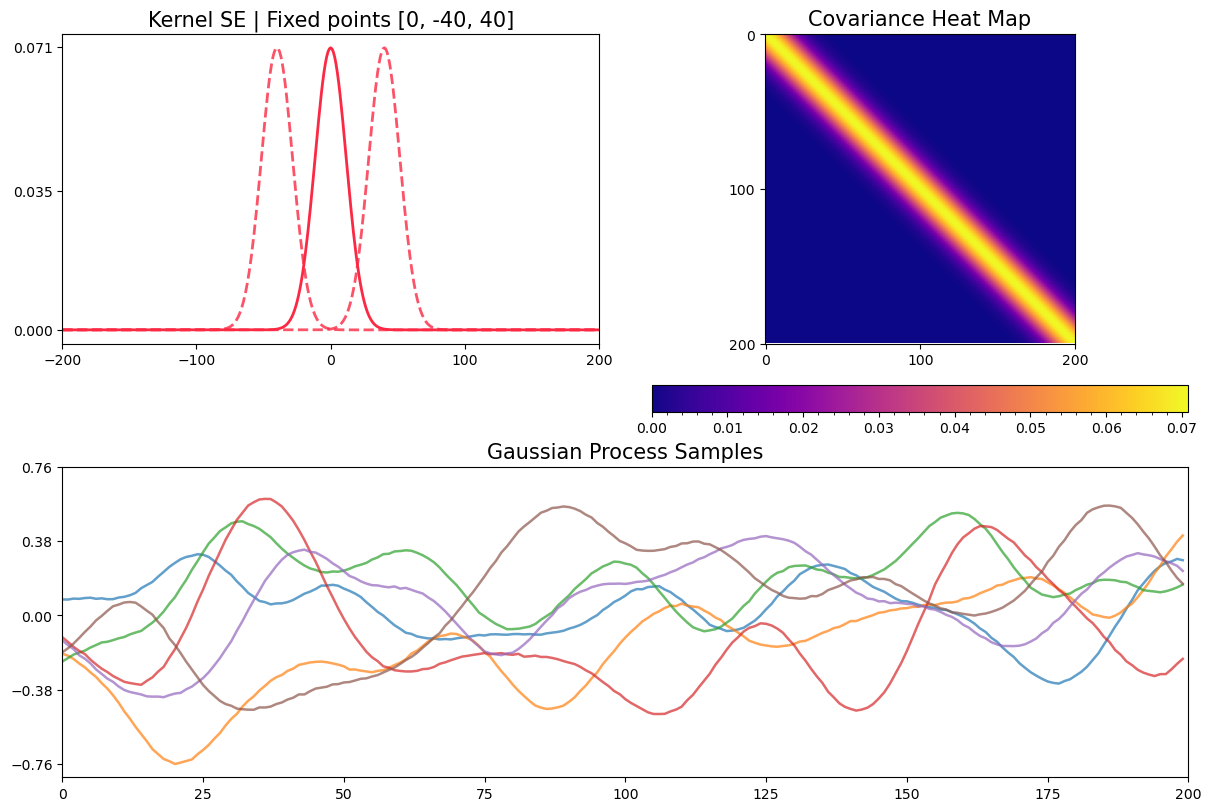
\includegraphics[scale=0.5]{k-SE}
	\caption{Representación gráfica del kernel exponencial cuadrático.}
\end{figure}

La construcción de \(k_{\mathrm{SE}}\) se puede realizar a partir de las funciones base
\begin{equation*}
	\phi_{c}(t) = \exp \left(-\frac{(t-c)^{2}}{2l^{2}}\right).
\end{equation*}
Si definimos la siguiente función de covarianza:
\[k(t_{p}, t_{q}) = \frac{\sigma_{p}^{2}}{N} \sum_{c=1}^{N} \phi_{c}(t_{p}) \phi_{c}(t_{q}),\]
y hacemos crecer la cantidad de puntos \(N\) a infinito, entonces se obtiene que
\begin{align*}
	\lim_{N \to \infty} \frac{\sigma_{p}^{2}}{N} \sum_{c=1}^{N} \phi_{c}(t_{p}) \phi_{c}(t_{q})	&= \sigma_{p}^{2} \int_{c_{\min}}^{c_{\max}} \phi_{c} (t_{p}) \phi_{c}(t_{q}) \dd{c} \\
																								&\to \sigma_{p}^{2} \int_{-\infty}^{\infty}\exp \left(-\frac{(t_{p} - c)^2}{2l^2}\right) \exp \left(-\frac{(t_{q} - c)^2}{2 l^2}\right) \dd{c} \\
	k(t_{p}, t_{q})																				&= \sqrt{\pi} l \sigma_{p}^{2} \exp \left(-\frac{(t_{p} - t_{q})^2}{2 (\sqrt{2} l)^2}\right).
\end{align*}
Como este kernel es isotrópico, entonces su densidad espectral también es isotrópica y gaussiana, como vimos en el primer capítulo.

\begin{proposition}
	La densidad espectral del kernel \(k_{\mathrm{SE}}(r)\) de parámetros \(h\) y \(l\) se escribe como
	\begin{equation*}
		S_{\mathrm{SE}}(s) = \frac{h}{\sqrt{2\pi} l} \exp \left(-2\pi^{2} l^{2} s^{2}\right).
	\end{equation*}
\end{proposition}

De forma análoga, si se tiene que una densidad espectral isotrópica tiene un dual de Fourier isotrópico, entonces ese dual es una función de covarianza. Esta densidad está en torno al origen, y si quisiéramos centrar la densidad espectral en torno a una frecuencia \(p\), debemos mantener la simetría en torno al origen para que sea válida. 

Veamos la siguiente construcción de densidad espectral en torno a la frecuencia \(p\), la cual genera el kernel conocido como Mixtura Espectral (\emph{Spectral Mixture} en inglés) que permite modelar comportamientos periódicos.

\begin{proposition}
	Consideremos la función gaussiana
	\[\phi_{p}(s) = \frac{1}{\sqrt{2\pi \sigma^2}} \exp \left(-\frac{(s - p)^{2}}{2\sigma^{2}}\right).\] Definiendo una densidad espectral de la forma \(S_{p}(s) = \frac{\phi_{p}(s) + \phi_{p}(-s)}{2}\), se tiene que su dual de Fourier es el kernel llamado \emph{Spectral Mixture}, un kernel estacionario de periodo \(p\), dado por
	\[k_{\mathrm{SM}}(r) = \exp \left(-2\pi^{2} \sigma^2 r^{2}\right) \cos(2\pi pr).\]
\end{proposition}

\begin{figure}[h]
	\centering
	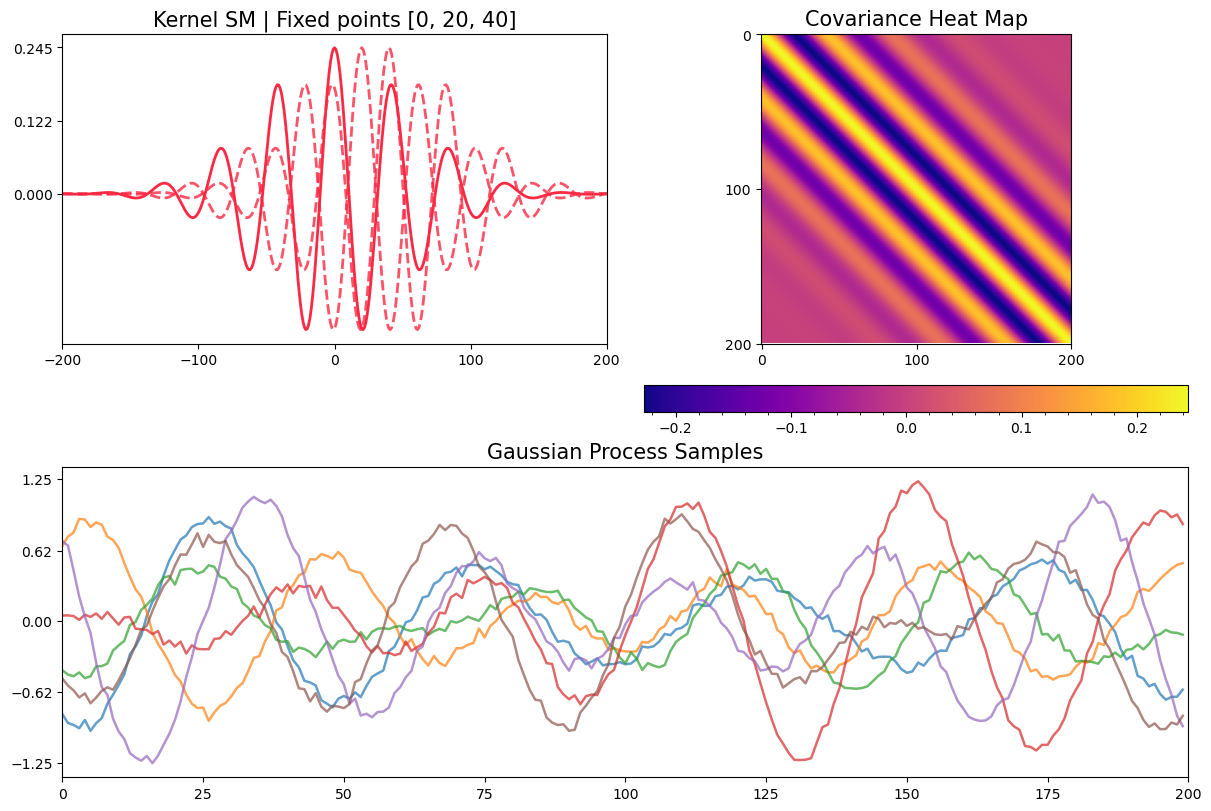
\includegraphics[scale=0.5]{k-SM}
	\caption{Representación gráfica del kernel spectral mixture.}
\end{figure}

La construcción anterior sigue siendo válida si consideramos varias frecuencias, incluso si consideramos el caso multidimensional no isotrópico.

\begin{proposition}
	Si se consideran \(N\) sumas de gaussianas multidimensional en \(\reals^{D}\)\cite{wilson2013gaussian}, entonces el kernel resultante es el \emph{Spectral Mixture} de \(N\) componentes.
	\begin{equation*}
		k(\bfr) = \sum_{q=1}^{N} \prod_{d=1}^{D} h_{q, d} \exp\left(-2\pi^{2} \sigma_{q, d}^{2} r_{d}\right) \cos(2\pi p_{q,d} r_{d}).
	\end{equation*}
\end{proposition}

Estos kernels permiten correlacionar puntos que estén a periodo \(\mu\) pero que no estén muy alejados, distancia controlada por el parámetro \(\sigma^2\). 

Un kernel que permite correlacionar los puntos que estén a periodo \(p\), de la misma forma independiente de la distancia de los puntos, es el kernel periódico definido como
\[ k_{\mathrm{Per}}(r) = h \exp \left(-\frac{2 \sen^{2}\left(\frac{\pi \vert r\vert}{p}\right)}{\ell^2}\right).\]

\begin{figure}[h]
	\centering
	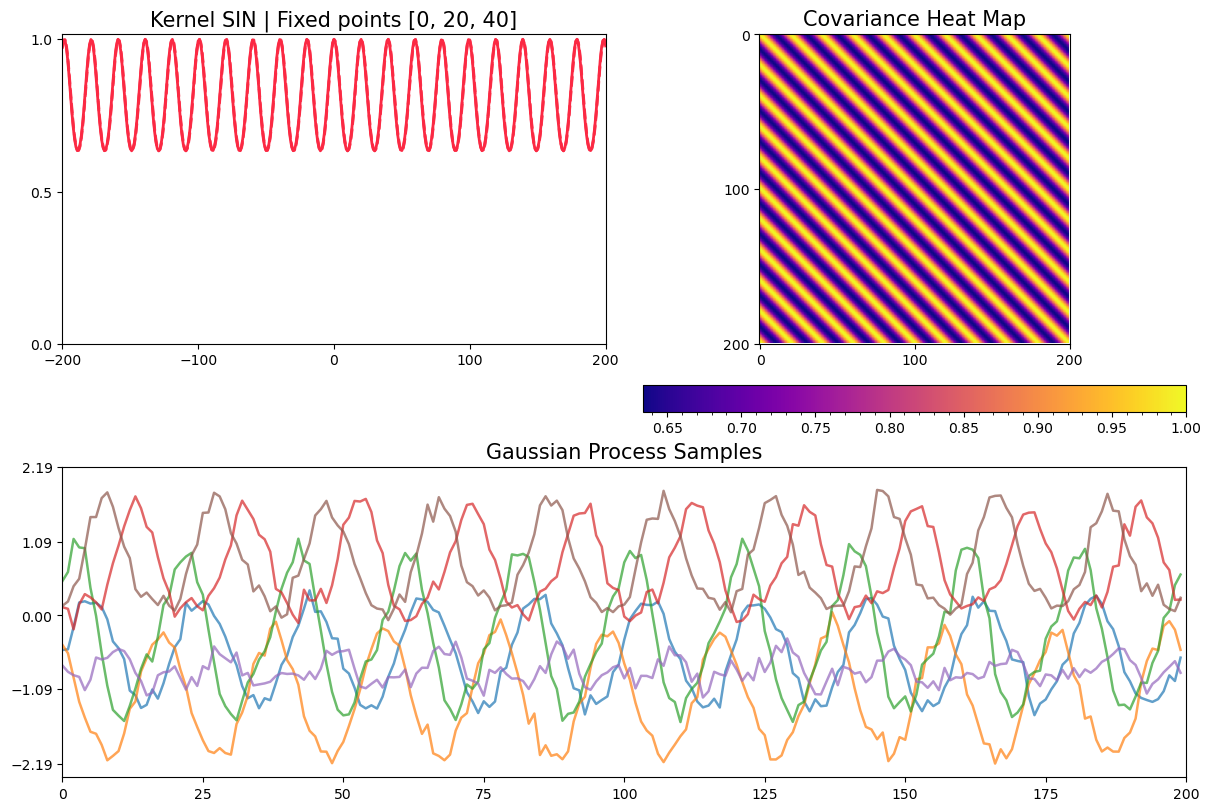
\includegraphics[scale=0.5]{k-SIN}
	\caption{Representación gráfica del kernel periódico.}
\end{figure}
El periodo \(p\) determina la distancia entre repetición de la función, y la escala \(\ell\) controla el nivel de correlación máxima.

Veamos algunos otros ejemplos de kernels estacionarios isotrópicos, destacando a la familia de kernels Matérn.
\begin{definition}
	Los kernels de Matérn depende de los parámetros \(v\) (la forma, \emph{shape} en inglés) y \(l\) (el largo, \emph{length} en inglés). Denotando \(\Gamma\) a la función gamma y \(K_{v}\) la función modificada de Bessel, estos kernels tienen la siguiente forma:
	\begin{equation*}
		k_{\mathrm{M}}(r) = h\frac{2^{1-v}}{\Gamma(v)} \left(\frac{\sqrt{2v} r}{l}\right)^{v} K_{v} \left(\frac{\sqrt{2v} r}{l}\right).
	\end{equation*}
\end{definition}

Dos de los casos más comunes son cuando \(v=3/2\) y \(v=5/2\):
\begin{align*}
	k_{v=3/2}(r)	&= h \left(1 + \frac{\sqrt{3} r}{l}\right) \exp \left(-\frac{\sqrt{3} r}{l}\right), \\
	k_{v=5/2}(r)	&= h \left(1 + \frac{\sqrt{5} r}{l} + \frac{5r^{2}}{3 l^{2}}\right) \exp \left(-\frac{\sqrt{5} r}{l}\right).
\end{align*}
En general, para todo parámetro \(v\) que cumpla \(v + \frac{1}{2} = p \in \naturals\), entonces la fórmula es un polinomio de grado \(p-1\) multiplicado por una exponencial. Esto indica a que mayor valor de \(v\), mayor es la suavidad del kernel. Más aún, cuando \(v \to \infty\), se tiene que este kernel converge a un exponencial cuadrático, es decir,
\begin{equation*}
	\lim_{n \to \infty} k_{v=n/2}(r) = k_{\mathrm{SE}}(r).
\end{equation*}

\begin{definition}
	Cuando \(v=1/2\), el kernel resultante es el exponencial, también conocido como el kernel de Laplace:
	\begin{equation*}
		k_{\mathrm{E}}(r) = h \exp \left(-\frac{r}{l}\right).
	\end{equation*}
\end{definition}

En dimensión \(1\), un proceso gaussiano con el kernel exponencial se llama el proceso de Ornstein-Uhlenbeck. 

\begin{figure}[h]
	\centering
	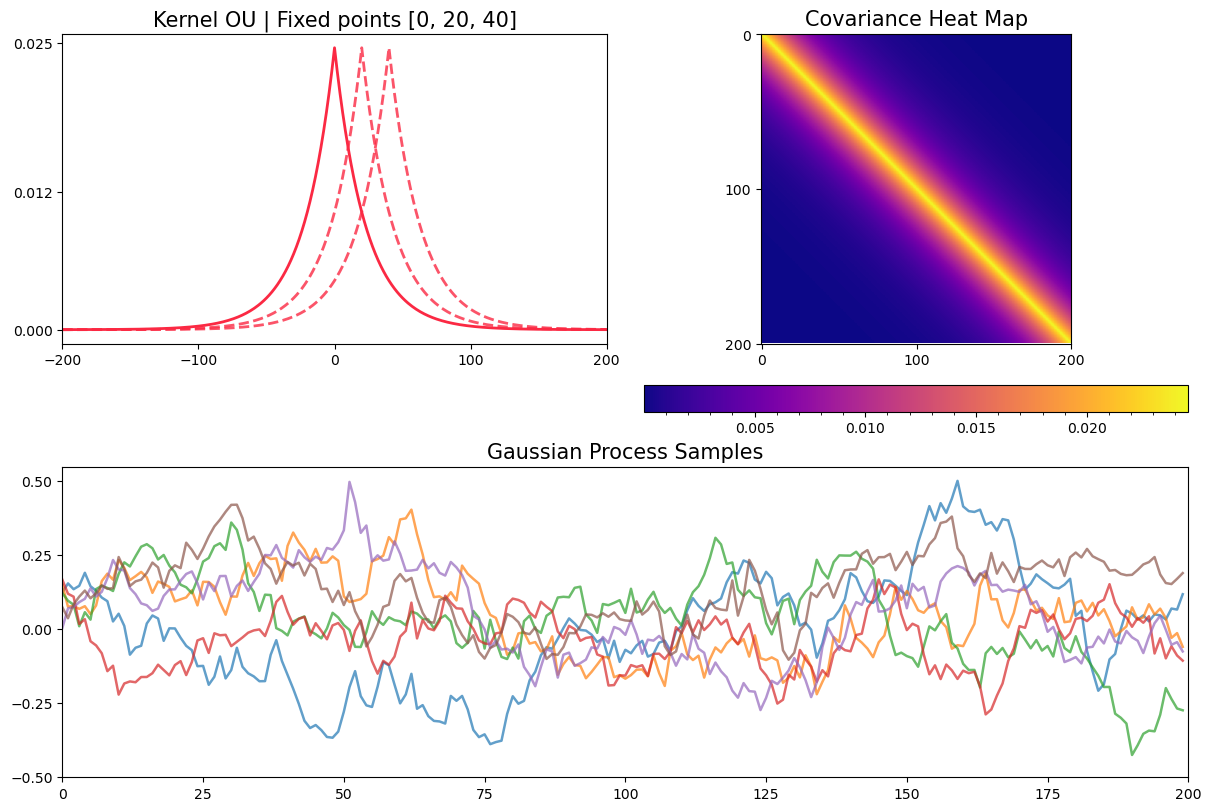
\includegraphics[scale=0.5]{k-OU}
	\caption{Representación gráfica del kernel de Laplace.}
\end{figure}

Veamos ahora una generalización del proceso exponencial y gaussiano.
\begin{definition}
	La familia \(\gamma\)-exponencial de kernels, para un valor de \(\gamma \in (0, 2]\), está dada por
	\begin{equation*}
		k_{\gamma}(r) = h \exp \left(-\left(\frac{r}{l}\right)^{\gamma}\right).
	\end{equation*}
\end{definition}

Ambas familia de kernels cumple una propiedades bastantes interesantes, ya que la suavidad de los procesos generados dependen de los parámetros de la familia del kernel. Ahora definiremos la noción de continuidad que utilizaremos para poder referirnos a la suavidad de un proceso.

\begin{definition}
	Diremos que el proceso \(\{x_{t}\}_{t \in \calI}\) es continuo en media cuadrática (\emph{mean-square} en inglés, y denotado MS-continuo) en un tiempo \(t\) si se cumple las siguientes dos condiciones:
	\begin{align*}
		\mean\left(\vert x_{t} \vert^{2}\right)							&< \infty, \\
		\lim_{s \to t} \mean\left(\vert x_{s} - x_{t}\vert^{2}\right)	&= 0.
	\end{align*}
\end{definition}

\begin{definition}
	Diremos que el proceso es diferenciable en media cuadrática (denotado MS-diferenciable) en un tiempo \(t\) si su derivada en dicho tiempo existe y se cumple que
	\begin{align*}
		\lim_{\triangle t \to 0} \mean\left( \left\vert \dv{x_{t}}{t} \right\vert^{2}\right)	&< \infty, \\
		\lim_{\triangle t \to 0} \mean\left( \left\vert \frac{x_{t + \triangle t} - x_{t}}{\triangle t} - \dv{x_{t}}{t} \right\vert^{2} \right) &= 0.
	\end{align*}

	De forma recursiva, diremos que un proceso es \(k\)-diferenciable en media cuadrática en un tiempo \(t\) si su \(k\)-ésima derivada en dicho tiempo existe, es continua en media cuadrática y cumple que:
	\begin{equation*}
	\lim_{\triangle t \to 0} \mean \left( \left\vert \frac{\dv[k-1]{x_{t + \triangle t}}{t} - \dv[k-1]{x_t}{t}}{\triangle t} - \dv[k]{x_{t}}{t} \right\vert^2\right) = 0.
	\end{equation*}
\end{definition}

Ahora que tenemos definida la noción de continuidad y diferenciabilidad en media cuadrática, veamos la suavidad de los diferentes procesos generados.
\begin{proposition}
	El proceso de Ornstein-Uhlenbeck es MS-continuo pero no es MS-dife\-ren\-ciable. El proceso con kernel \(\gamma\)-exponencial no es MS-diferenciable salvo cuando \(\gamma = 2\), en cuyo caso es infinitamente MS-diferenciable. El proceso de Matérn con parámetro \(v\) es \(\lceil v-1 \rceil\) veces MS-diferenciable.
\end{proposition}

De las familias \(\gamma\)-exponencial y Matérn con parámetro \(v\), el kernel SE es el único que cumple la propiedad de ser infinitamente MS-diferenciable. Existen otros kernels con esta propiedad, entre los cuales destaca el kernel conocido racional cuadrático. Veamos a continuación su definición y cómo se puede interpretar.

\begin{definition}
	El kernel racional cuadrático (\emph{rational quadratic} en inglés, denotado RQ) de parámetros \(\alpha > 0\) (la forma, \emph{shape} en inglés) y \(l > 0\) (el largo, \emph{length} en inglés) se define como
	\[ k_{\mathrm{RQ}}(r) = h \left(1 + \frac{r^2}{2\alpha l^2}\right)^{-\alpha}.\]
\end{definition}

\begin{figure}[h]
	\centering
	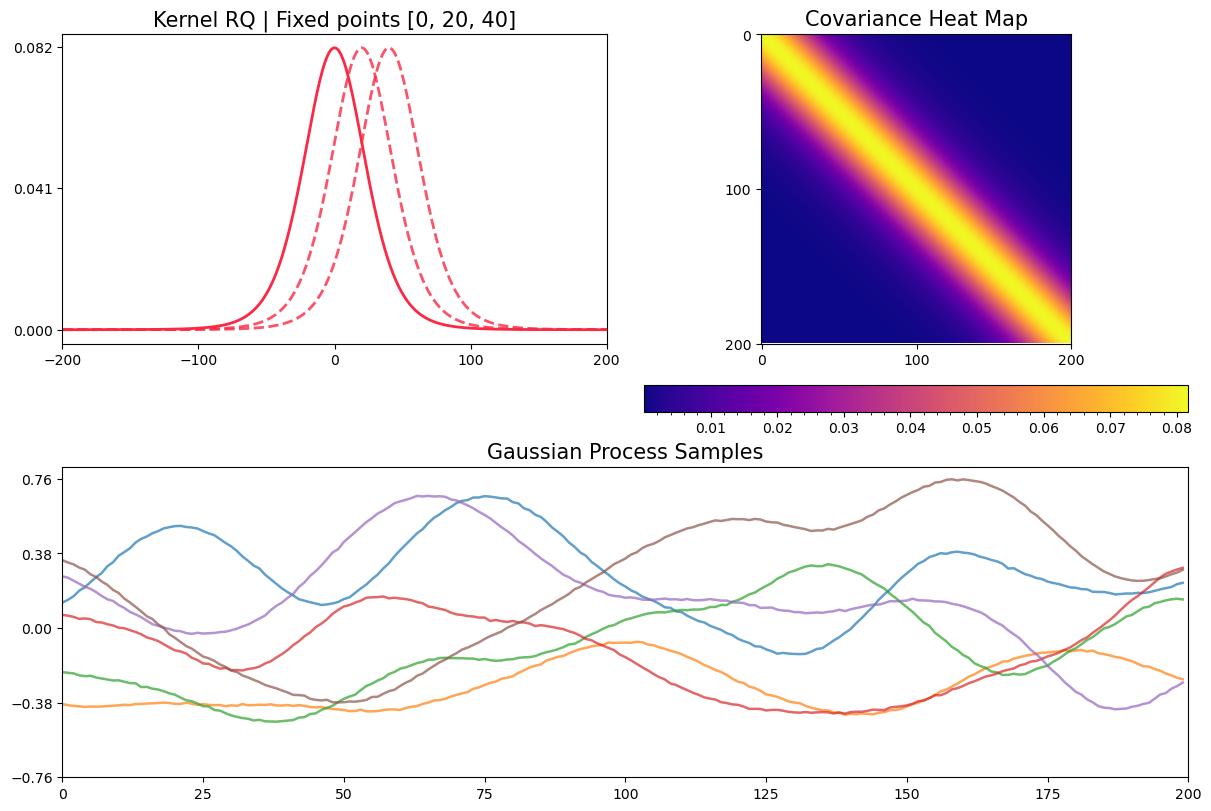
\includegraphics[scale=0.5]{k-RQ}
\end{figure}

El kernel RQ puede verse como una suma infinita de kernels SE con diferentes escalas \(l\), donde el parámetro \(\alpha\) determina el peso relativo, o proporción, entre variaciones de alta o baja escala. Si parametrizamos como \(\tau = l^{-2}\) con una distribución gamma \(p (\tau \mid \alpha, \beta) \propto \tau^{\alpha - 1} \exp (-\alpha \tau / \beta )\), entonces integrando un kernel SE con respecto \(\tau\) se tiene que
\begin{align*}
	k_{\mathrm{RQ}}(r)	&= \int p(\tau \mid \alpha, \beta) k_{\mathrm{SE}}(r \mid \tau) \dd{\tau} \\
						&\propto \int \tau^{\alpha-1} \exp \left(-\alpha \frac{\tau}{\beta} \right) \exp \left(-r^{2} \frac{\tau}{2}\right) \dd{\tau} \\
						&\propto \left(1 + \frac{r^{2}}{2\alpha l^{2}}\right)^{-\alpha},
\end{align*}
con \(\beta = l^{-2}\). Con esta construcción, y usando el hecho de que el operador derivada conmuta con la integral, es directo ver que este kernel hereda la suavidad del kernel SE. Además, a medida de que \(\alpha\) tiende a infinito, el kernel RQ converge a un kernel SE:
\begin{equation*}
	\lim_{\alpha \to \infty} \sigma^2 \left(1 + \frac{r^{2}}{2\alpha l^{2}}\right)^{-\alpha} = \sigma^2 \exp\left(\frac{r^{2}}{2 \ell^{2}}\right).
\end{equation*}

\begin{proposition}
	El proceso generado con un kernel RQ es infinitamente MS-diferencia\-ble, para cualquier \(\alpha > 0\).
\end{proposition}

Todos los kernels mostrados hasta ahora son isotrópicos. Sin embargo, todos los kernels isotrópicos \(k_{r}\) puedes convertirse a anisotrópicos reemplazando \(r^{2}\) por una función que depende de una matriz semidefinida positiva \(M\) tal que
\begin{equation*}
	k_{r} \left(r^{2}(t, \bar{t})\right) = k_{r}\left((t-\bar{t})^{\top} M (t-\bar{t})\right).
\end{equation*}
Si \(M\) es una matriz diagonal, entonces el kernel escala cada dimensión de forma independiente. La transformación más general es de la siguiente forma:

\begin{proposition}
	Dado un kernel isotrópico \(k_{r}\), se define el kernel
	\begin{align*}
		k_{M} (t, \bar{t})	&= k_{r}\left((t - \bar{t})^{\top} M (t-\bar{t}) \right), \\
		M					&= \Lambda \Lambda^{\top} + \Psi,
	\end{align*}
	donde \(\Lambda\) es una matriz de dimensión \(D \times k\), sus columnas definen \(k\) direcciones de gran relevancia, y \(\Psi\) es una matriz diagonal positiva que captura la relevancia de cada dimensión. El kernel \(k_{M}\) es un kernel estacionario anisotrópico.
\end{proposition}

\subsection{Kernels de Producto Interno}

Todos los kernels estudiados hasta ahora cumplen la propiedad de ser estacionarios. En muchos casos, el proceso que se desea estimar no cumple con el supuesto de estacionalidad, al tener una componente no estacionaria. Una forma de modelar dicha componente es con una función de media. Otro enfoque es considerar kernels no estacionarios, donde la familia más destacada son aquellos con forma de producto punto.

El kernel de producto punto más simple es el kernel lineal, definido como
\[ k_{\mathrm{Lin}} (t, \bar{t}) = \sigma_{0}^{2} + \langle t, \bar{t}\rangle.\]

\begin{figure}[h]
	\centering
	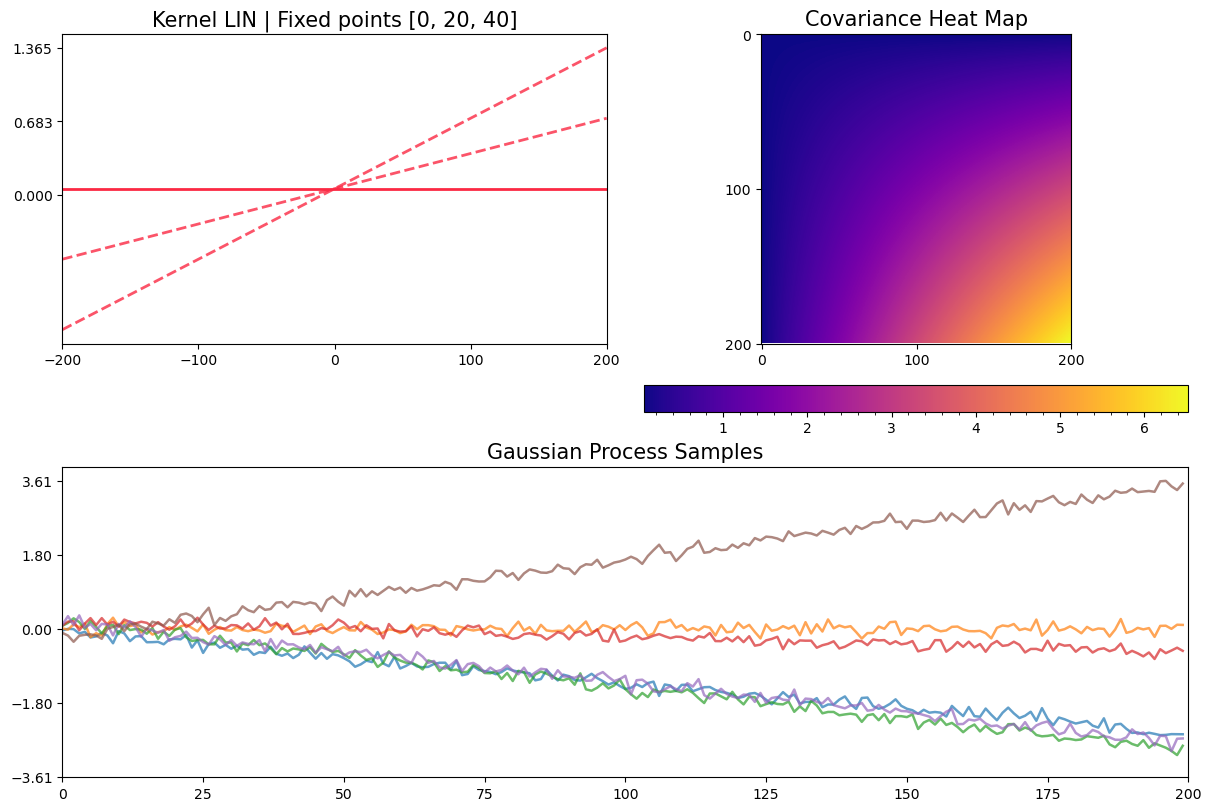
\includegraphics[scale=0.5]{k-LIN}
	\caption{Representación gráfica del kernel lineal.}
\end{figure}

Este kernel que permite modelar dependencias lineales con respecto a las variables de entrada, y se le conoce como Regresiones Lineales Bayesianas. Si \(\sigma_{0}^{2} = 0,\) entonces se dice kernel lineal homogéneo. Como es un producto punto, es posible incluir una matriz definida positiva \(\Sigma_{p}\) entre las componentes de \(t\), de la misma forma que se construyen los kernels anisotrópicos, quedando el kernel lineal generalizado como
\begin{align*}
	k_{\mathrm{Lin}} (t, \bar{t})	&= \sigma_{0}^{2} + t^{\top} \Sigma_{p} \bar{t},\\
	\Sigma_{p}						&= \Lambda \Lambda^{\top} + \Psi.
\end{align*}
Con el kernel lineal es posible incluir dependencias lineales. Es natural pensar en kernels que nos permitan modelar otro tipo de dependencias, tales como cuadráticas o polinomiales en general. Para esto, definamos el kernel polinomial de grado \(n\).

\begin{definition}
	El kernel polinomial \(k_{n} (t, \bar{t}) = \left(\sigma_{0}^{2} + t^{\top} \Sigma_{p} \bar{t}\right)^{n}\) es una función de covarianza válida para \(n \in \naturals^+\).
\end{definition}

Para ver que este kernel es una función de covarianza válida, basta con poder expresarlo en forma de producto punto. Por simplicidad, consideremos el caso isométrico homogéneo:
\begin{align*}
	k_{n}(t, \bar{t})	&= \langle x, \bar{t} \rangle^{n} \\
						&= \left(\sum_{d=1}^{D} t_{d} \bar{t}_{d}\right)^{n}\\
						&= \prod_{i=1}^{n} \left(\sum_{d=1}^{D} t_{d} \bar{t}_{d}\right) \\
						&= \sum_{d_{1}=1}^{D} \dotsb \sum_{d_{n}=1}^{D} \left(\prod_{i=1}^{n} t_{d_{i}}\right) \left(\prod_{i=1}^{n} \bar{t}_{d_{i}}\right)\\
						&= \langle \bfphi(t), \bfphi(\bar{t}) \rangle.
\end{align*}
A priori, se pensaría que la suma tiene \(D^{n}\) términos, pero como el orden de las multiplicaciones \(t_{d_{1}}, \dotsc, t_{d_{n}}\) conmuta, es posible reducir el número de términos definiendo un vector \(\bfm = (m_1, \dotsc, m_D)\), donde la componente \(m_{d}\) especifica el número de veces que la componente \(t_{d}\) aparece en el monomio bajo la restricción de que \(\sum_{i=1}^{D} m_{i} = n\). La función \(\bfphi(t)\) está definida por componentes indexadas por los vectores \(\bfm\), donde la función característica \(\phi_{\bfm}(t)\) es proporcional al monomio \(t_{1}^{m_{1}}, \dotsc, t_{D}^{m_{D}}\) y degenerada en \(\frac{n!}{m_{1}! \dotsb m_{D}!}\):
\begin{equation*}
	\phi_{\bfm}(t) = \sqrt{\frac{n!}{m_{1}!...m_{D}!}} t_{1}^{m_{1}} \dotsb t_{D}^{m_{D}}.
\end{equation*}
Esto implica que las funciones generadas son combinaciones lineales de los monomios de todos los órdenes, produciendo cualquier polinomio homogéneo de orden \(n\). Si al espacio de entrada le agregamos una coordenada constante \(t_{0} = 1\), entonces es posible reproducir cualquier polinomio de orden hasta \(n\). De forma equivalente, en vez de agregar una coordenada constante basta con sumar una constante \(\sigma_{0}^{2}\) antes de elevar a \(n\). El kernel polinomial cumple la propiedad que la varianza crece rápidamente a medida que \(\vert x \vert\) crece, pero si los datos están normalizados entonces este kernel entrega buenos resultados.

Siguiendo este mismo enfoque, podemos construir la función \(\bfphi\) con cualquier base finita de funciones, generando funciones utilizando dicha base. La construcción más simple es considerar un hiperparámetro por cada elemento de la base, con el fin de determinar cuales funciones son relevantes.
\begin{definition}
	Dada una base de funciones \(\Phi = \{\phi_{i}\}_{i=1}^{N}\), el kernel máquina de relevancia vectorial (\emph{relevance vector machine} en inglés, denotado RVM) es de la forma
	\begin{equation*}
		k_{\mathrm{RVM}}(t, \bar{t}) = \sum_{j=1}^{N} \frac{1}{\alpha_{j}} \phi_{j}(t) \phi_{j}(\bar{t}).
	\end{equation*}
\end{definition}

\begin{proposition}
	El kernel RVM es una función de covarianza degenerada (el espacio de características es finito-dimensional).
\end{proposition}

A medida de que el término \(\alpha_{j}\) se acerque a infinito, la componente \(\phi_{j}\) tiene menos relevancia en la covarianza del proceso, mientras que los términos cercanos a cero explican la mayor parte de la varianza. A su vez, podemos generalizar la expresión anterior utilizando la matriz definida positiva \(\Sigma_{p} = \Lambda \Lambda^{\top} + \Psi\), produciendo el kernel de forma
\begin{align*}
	k_{\Sigma_{p}}(t, \bar{t})	&= \bfphi(t)^{\top} \Sigma_{p} \bfphi(\bar{t}) \\
								&= \sum_{i=1}^{N} \sum_{j=1}^{N} \sigma_{ij} \phi_{i}(t) \phi_{j}(\bar{t}).
\end{align*}

\subsection{Otros Kernels de Covarianza}
Existen funciones de covarianza que no son estacionarias y tampoco tienen forma de producto punto. Un ejemplo clásico es el kernel que produce el movimiento browniano o el kernel producto.

\begin{proposition}
	El proceso de Wiener con función de covarianza \(k(t, \bar{t}) = \min \{x, \bar{t}\}\) es un proceso no estacionario.
\end{proposition}

\begin{figure}[h]
	\centering
	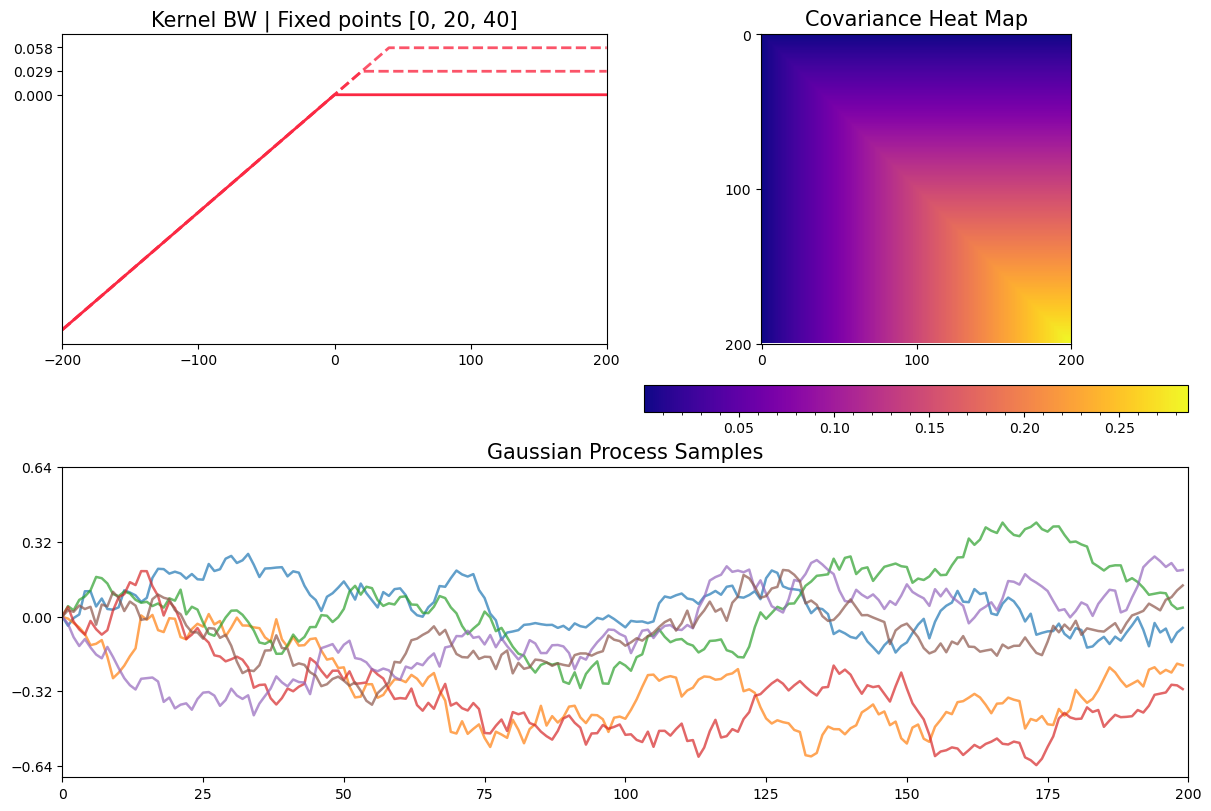
\includegraphics[scale=0.5]{k-BW}
	\caption{Representación gráfica del kernel browniano.}
\end{figure}

\begin{proposition}
	El proceso de ruido blanco (\emph{white noise} en inglés) con función de covarianza \(k(t, \bar{t}) = \delta_{x, \bar{t}}\) es un proceso no estacionario.
\end{proposition}

Existen muchos otros kernels válidos que pueden construirse utilizando funciones no lineales, las cuales se aplican después de operar \(t\) con \(\bar{t}\). Un ejemplo es el kernel red neuronal (\emph{neural network kernel} en inglés) definido como
\begin{equation*}
	k_{\mathrm{NN}}(t, \bar{t}) = \frac{2}{\pi} \arcsin \left(\frac{2x^{\top} \Sigma_{p}\bar{t}}{\left(1 + 2x^{\top} \Sigma_{p} \bar{t}\right) \left(1 + 2x^{\top} \Sigma_{p} \bar{t}\right)}\right).
\end{equation*}
Este kernel es válido y es no estacionario. Sin embargo, no todas las funciones generan kernels válidos, por ejemplo el kernel sigmoide
\begin{equation*}
	k(t, \bar{t}) = \tanh(a + b \langle x, \bar{t}\rangle),
\end{equation*}
no es definida positiva para ningún valor de \(a\) y \(b\). Otro kernel no estacionario válido es el kernel de base gaussiana, definido como
\begin{align*}
	k_{\mathrm{GB}}(t, \bar{t})	&= \frac{1}{(2\pi \sigma_u^2)^{d/2}} \int \exp\left(-\frac{\vert x-u \vert^2}{2\sigma_g^2} - \frac{\vert \bar{t}-u \vert^2}{2\sigma_g^2} -\frac{\langle u, u\rangle}{2\sigma_u^2}\right) \dd{u} \\
								&= \left(\frac{\sigma_e}{\sigma_u}\right)^d \exp\left(-\frac{\langle x, x \rangle}{2 \sigma_m^2}\right) \exp\left(-\frac{\vert x-\bar{t}\vert^2}{2\sigma_s^2}\right) \exp\left(-\frac{\langle \bar{t}, \bar{t}\rangle}{2\sigma_m^2}\right), \\
\end{align*}
donde
\begin{align*}
	\frac{1}{\sigma_{e}^{2}}	&=\frac{2}{\sigma_{g}^{2}}+\frac{1}{\sigma_{u}^{2}},\\
	\sigma_{s}^{2}				&= 2\sigma_{g}^{2}+\frac{\sigma_{g}^{4}}{\sigma_{u}^{2}},\\
	\sigma_{m}^{2}				&= 2\sigma_{u}^{2}+\sigma_{g}^{2}.
\end{align*}
Este kernel converge al exponencial cuadrático cuando \(\sigma_{u}^{2} \to \infty\), por lo que podemos interpretar que el término \(\sigma_{u}^{2}\) controla el grado de no estacionalidad.

Otra forma de crear kernels es a partir de kernels estacionarios. Si \(u\) es una función de características no lineal y \(k_{u}(u, \bar{u})\) es un kernel estacionario en \(u\), entonces
\begin{equation*}
	k_{t, u}(t, \bar{t}) = k_{u}(u(t), u(\bar{t})),
\end{equation*}
es un kernel para \(t\). Consideremos el caso en que \(u(t) = (\cos(t), \sen(t))\) y \(k_{u}\) es SE, entonces
\begin{equation*}
	k_{t, u}(t, \bar{t}) = \exp \left(-\frac{2\sen^{2}\left(\frac{x-\bar{t}}{2}\right)}{\ell^{2}}\right)
\end{equation*}
coincide con el kernel periódico. Es posible construir kernels de forma más complejas pero que conserven la propiedad de definido positivo. Un ejemplo es el kernel de la forma
\begin{equation*}
	k(t, \bar{t}) = \prod_{d=1}^{D} \left(\frac{2\ell_{d}(t) \ell_{d}(\bar{t})}{\ell_{d}^{2}(t) + \ell_{d}^{2}(\bar{t})}\right) \exp\left(-\sum_{d=1}^{D} \frac{(t_{d}-\bar{t}_{d})^{2}}{\ell_{d}^{2}(t) + \ell_{d}^{2}(\bar{t})}\right),
\end{equation*}
donde cada \(\ell_{d}\) es una función positiva de \(t\), es una función de covarianza que para todo \(t\) cumple \(k(t, t) = 1\). Otro ejemplo es considerar un kernel \(k_{S}\) estacionario e isotrópico, y una función \(\Sigma\) a valores matriciales de dimensión \(D \times D\) definida positiva. Luego el kernel
\begin{equation*}
	k_{\mathrm{NS}}(t, \bar{t}) = \frac{2^{\frac{D}{2}} \vert \Sigma(t) \vert^{\frac{1}{4}} \vert \Sigma(\bar{t}) \vert^{\frac{1}{4}}}{\vert \Sigma(t) + \Sigma(\bar{t}) \vert^{\frac{1}{2}}} k_{S}\left(\left((t-\bar{t})^{\top} \left(\frac{\Sigma(t) + \Sigma(\bar{t})}{2}\right) (t-\bar{t})\right)^{\frac{1}{2}}\right),
\end{equation*}
es una función de covarianza no estacionaria.


\section{Composición de Kernels}

En la sección anterior revisamos las familias de kernels más comunes. Es posible construir nuevos kernels a partir de un kernel base y funciones auxiliares. Veamos a continuación algunas formas de construir kernels que mantienen la propiedad de ser definido positivo.

\subsection{Composición con funciones auxiliares}

La forma más simple de construir kernels es partir desde un único kernel base, para luego componerlo con alguna función auxiliar. Veamos a continuación las composiciones válidas.

\begin{proposition}
	Sea \(k\) un kernel definido positivo, \(n \in \naturals\), \(u\) una función unaria y \(h\) una función binaria (ambas funciones arbitrarias). Entonces las siguientes construcciones producen kernels válidos:
	\begin{itemize}
		\item Potencia: \(\tilde{k}(t, \bar{t}) = k^{n}(t, \bar{t})\).
		\item Normalización: \(\tilde{k}(t, \bar{t}) = \frac{k(t, \bar{t})}{\sqrt{k(t, t)} \sqrt{k(\bar{t}, \bar{t})}}\).
		\item Escalamiento: \(\tilde{k}(t, \bar{t}) = u(t) k(t, \bar{t}) u(\bar{t})\).
		\item Composición: \(\tilde{k}(t, \bar{t}) = k(u(t), u(\bar{t}))\).
		\item Convolución: \(\tilde{k}(t, \bar{t}) = \int \int h(t, s) k(s, \bar{s}) h(\bar{t}, \bar{s}) \dd{s} \dd{\bar{s}}\).
		\item Reflexión: \(\tilde{k}(t, \bar{t}) = k(t, \bar{t}) + k(-t, \bar{t}) + k(t, -\bar{t}) + k(-t, -\bar{t})\).
	\end{itemize}
\end{proposition}

Cada una de estas construcciones produce funciones con alguna propiedad. Por ejemplo, si \(f(t) \sim \GP(0, k)\), entonces el escalamiento produce funciones de la forma \(f(t) u(t)\), la composición funciones de la forma \(f(u(t))\), la potencia funciones de la forma \(f^{n}(t)\), la convolución funciones de la forma \(\tilde{f}(t) = \int f(s) h(s, t) \dd{s}\) y la reflexión permite generar funciones simétricas \(\tilde{f}(t) = \tilde{f}(-t) = f(t) + f(-t)\).

\subsection{Composición entre Kernels}

Además de manipular un único kernel para obtener otro diferente, también es posible componer kernels entre sí, manteniendo la propiedad de ser definido positivo \cite{12} \cite{13}. Veamos las operaciones de
composición válidas entre kernels.

\begin{proposition}
	Sean \(k_{1}\) y \(k_{2}\) dos kernels de covarianza. Entonces las siguientes composiciones producen kernels válidos.
	\begin{itemize}
		\item Suma: \(k(t, \bar{t}) = k_{1}(t, \bar{t}) + k_{2}(t, \bar{t})\).
		\item Producto: \(k(t, \bar{t}) = k_{1}(t, \bar{t}) k_{2}(t, \bar{t})\).
		\item Punto de Cambio (\emph{Changepoint} en inglés):
		\[k(t, \bar{t}) = \sigma(t) k_{1}(t, \bar{t}) \sigma(\bar{t}) + (1-\sigma(t)) k_{2}(t, \bar{t}) (1 - \sigma(\bar{t})),\]
		donde \(\sigma(t) = (1 + e^{-x})^{-1}\) o alguna función creciente de \(0\) a \(1\).
	\end{itemize}
\end{proposition}

Cada una de estas composiciones produce un efecto distinto. Una forma de interpretar la composición de kernels es utilizando su representación de producto punto en el espacio de componentes. Consideremos \(k_{1}(t, \bar{t}) = \bfphi_{1}(t)^{\top} \bfphi_{1}(\bar{t})\) y \(k_{2}(t, \bar{t}) = \bfphi_{2}(t)^{\top} \bfphi_{2}(\bar{t})\). Luego la suma se puede expresar como
\begin{align*}
	k_{1}(t, \bar{t}) + k_{2}(t, \bar{t})	&= \bfphi_{1}(t)^{\top} \bfphi_{1}(\bar{t}) + \bfphi_{2}(t)^{\top} \bfphi_{2}(\bar{t}) \\
											&= \begin{bmatrix} \bfphi_{1}\left(t\right) \\ \bfphi_{2}\left(t\right) \end{bmatrix}^{\top} \begin{bmatrix} \bfphi_{1}(\bar{t}) \\ \bfphi_{2}(\bar{t}) \end{bmatrix},
\end{align*}
la cual coincide con concatenar las dimensiones del espacio de características. A su vez, la multiplicación se puede expresar como
\begin{align*}
	k_{1}(t, \bar{t}) k_{2}(t, \bar{t})	&= \left( \bfphi_{1}^{\top}(t) \bfphi_{1}(\bar{t}) \right) \left(\bfphi_{2}(t)^{\top} \bfphi_{2}(\bar{t}) \right) \\
										&= \left(\sum_{i} \phi_{1}^{(i)}(t) \phi_{1}^{(i)}(\bar{t})\right) \left(\sum_{j} \phi_{2}^{(j)}(t) \phi_{2}^{(j)}(\bar{t})\right) \\
										&= \sum_{i, j} \left(\phi_{1}^{(i)}(t) \phi_{2}^{(i)}(\bar{t})\right) \left(\phi_{1}^{(j)}(t) \phi_{2}^{(j)}(\bar{t}) \right),
\end{align*}
la cual coincide con multiplicar las dimensiones del espacio de características.

Otra interpretación posible surge desde el espacio de las funciones generadas por cada proceso. La suma de kernels se interpreta como la superposición de procesos independientes, cada uno correspondiente a uno de los kernels en la suma. Esto se deduce del siguiente resultado.
\begin{figure}[h]
	\centering
	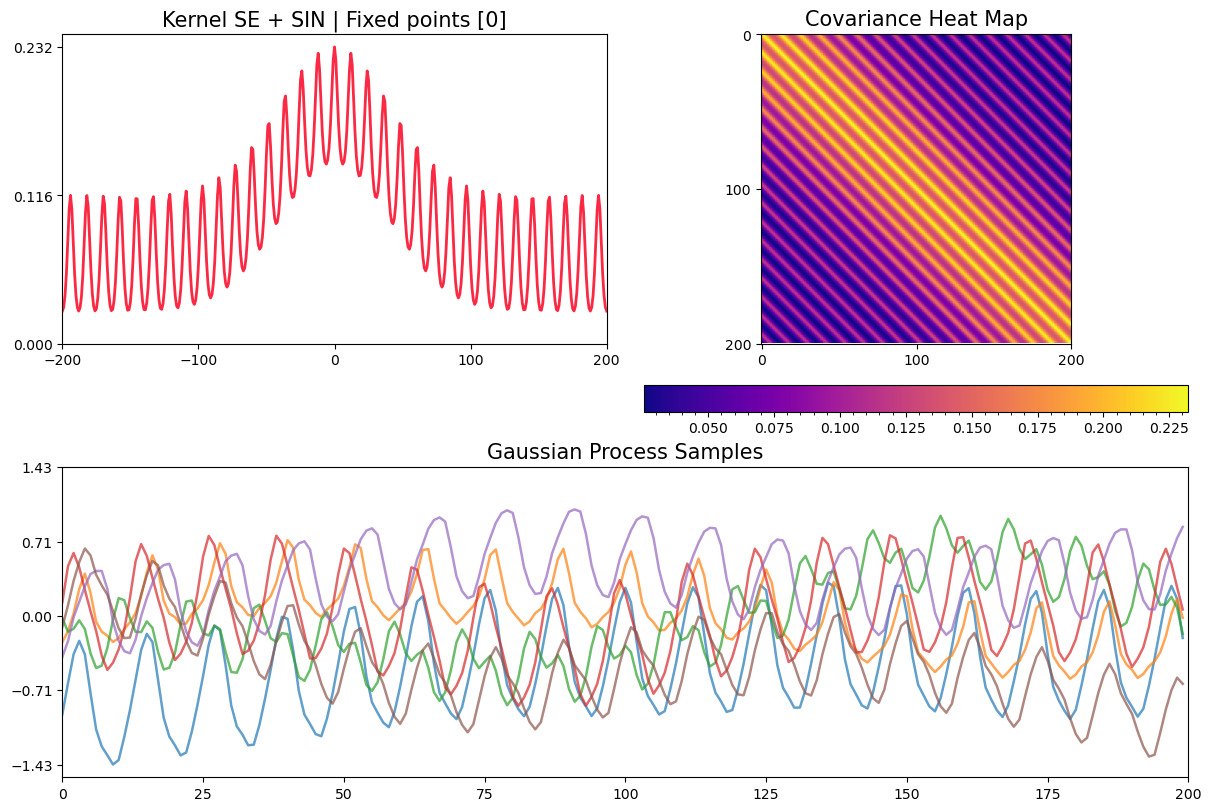
\includegraphics[scale=0.5]{k-SE+SEN}
	\caption{Representación gráfica de la suma de kernels SE + SEN.}
\end{figure}

\begin{proposition}
	Sean \(f_{1} \sim \GP(\mu_{1}, k_{1})\) y \(f_{2} \sim \GP(\mu_{2}, k_{2})\) dos GP independientes. Entonces la suma es un GP de la forma
	\begin{equation*}
		f = f_{1} + f_{2} \sim \GP(\mu_{1} + \mu_{2}, k_{1} + k_{2}).
	\end{equation*}
\end{proposition}

El resultado permite poder descomponer la función \(f\) en las componentes \(f_{1}\) y \(f_{2}\). Sean \(T, \bff\) los datos observados. Si suponemos que \(\bff = \bff_{1} + \bff_{2}\), entonces podemos estimar \(\bff_{1}\) (y \(\bff_{2}\)) utilizando la distribución posterior de \(f_{1}\) (y \(f_{2}\)) dado \(f\):
\begin{equation*}
	\bar{\bff}_{1} \mid \bff, T, \bar{t} \sim \calN\left(\bar{\mu}_{1} + \bar{\bfk}_{1}^{\top} (\mathbf{K}_{1} + \mathbf{K}_{2})^{-1} (\bff - \mu_{1} - \mu_{2}), \bar{\mathbf{K}}_{1} - \bar{\bfk}_{1}^{\top} (\mathbf{K}_{1}
	+ \mathbf{K}_{2})^{-1} \bar{\bfk}_{1}\right)
\end{equation*}
donde \(\mathbf{K}_{i} = k_{i}(T, T)\), \(\bar{\mathbf{K}}_{1} = k_{1}(\bar{t}, \bar{t})\) y \(\bar{\bfk}_{1} = k_{1}(\bar{t}, T)\). Si se modela \(f\) como \(\GP(0, k_{1} + \dotsb + k_{n})\), entonces es posible descomponer \(f\) en la suma \(f_{1} + \dotsb + f_{n}\), donde sus respectivas posteriores tienen la siguiente forma:
\begin{align*}
	f_{d}(\bar{t})	&\sim \calN\left(\mu_{d}, \sigma_{d}^{2}\right), \text{ para } d=1, \dotsc, n,\\
	\mu_{d}			&= k_{d}(\bar{t}, T) \left[ \sum_{i=1}^{n} k_{i}(T, T) \right]^{-1} f(t), \\
	\sigma_{d}^{2}	&= k_{d}(\bar{t}, \bar{t}) - k_{d}(\bar{t}, T) \left[ \sum_{i=1}^{n} k_{i}(T, T) \right]^{-1} k_{d}(T, \bar{t}).
\end{align*}

Por otro lado, el producto de kernels es considerado como una operación \textsc{AND}, ya que para que \(t\) y \(\bar{t}\) estén correlacionados deben estarlo bajo el criterio de ambos kernels \(k_{1}\) y \(k_{2}\). Los efectos que se logran al multiplicar kernels dependen del kernel escogido. Veamos los siguientes efectos:

\begin{itemize}
	\item Sea \(k\) un kernel que tiene una estructura de correlación global (como el caso lineal). Al multiplicarlo por un kernel SE se remueven las correlaciones lejanas, ya que decrece monótamente a medida de que la distancia crece.
	\item Sea \(k\) un kernel que genera las funciones \(f(t) \sim \GP(0, k)\). Al multiplicar dicho kernel con un kernel LIN las funciones generadas corresponden a las originales multiplicadas por un término en \(t\), es decir, \(t f(t) \sim \GP(0, k k_{\mathrm{Lin}})\).
	\item Sea \(k\) un kernel que genera las funciones \(f(t) \sim \GP(0, k)\). Al multiplicar dicho kernel con un kernel PER las funciones generadas corresponden a las originales multiplicadas por una función periódica independiente, es decir, \(f(t) f_{\mathrm{Per}}(t) \sim \GP(0, k k_{\mathrm{Per}})\), donde \(f_{\mathrm{Per}} \sim \GP(0, k_{\mathrm{Per}})\).
\end{itemize}

\begin{figure}[h]
	\centering
	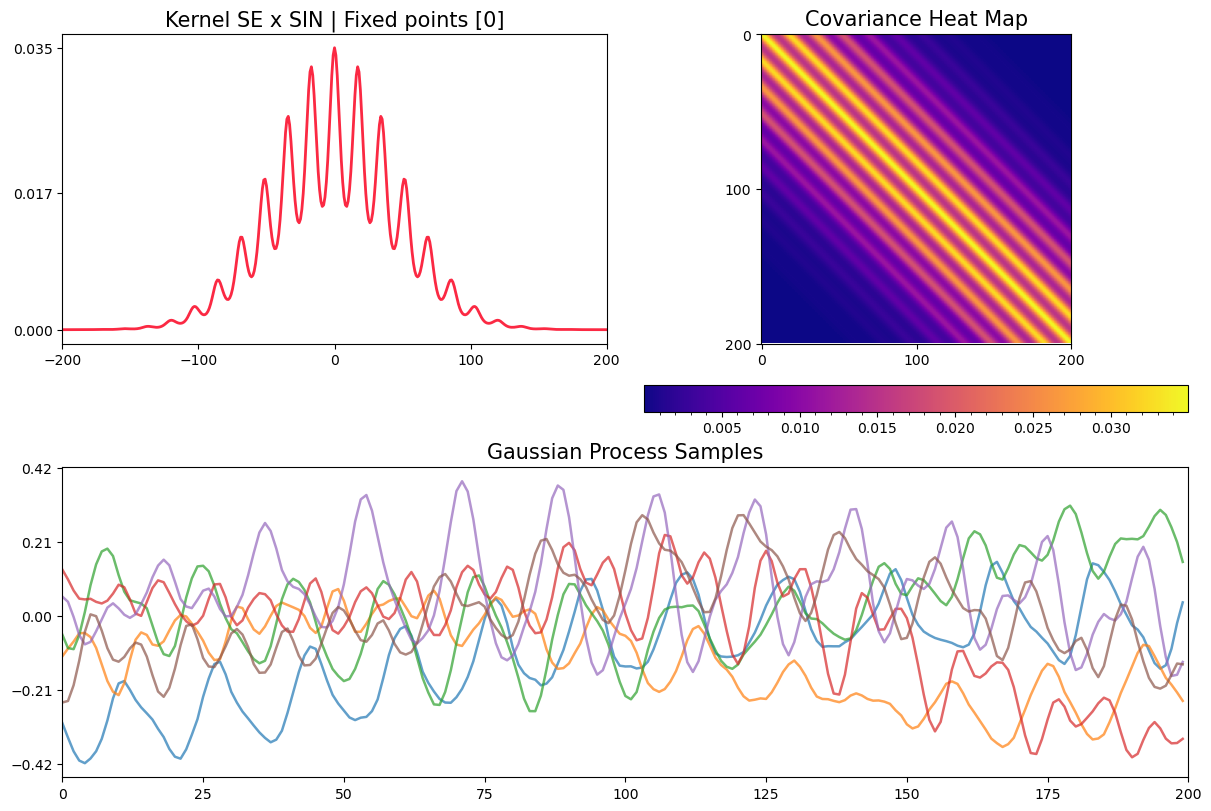
\includegraphics[scale=0.5]{k-SE-SEN}
	\caption{Representación gráfica de la multiplicación de kernels SE * SEN.}
\end{figure}

La composición del tipo \emph{changepoint} entre los kernels \(k_{1}\) y \(k_{2}\) entrega el kernel \(\CP(k_{1}, k_{2})\), que se mueve de un kernel al otro dependiendo una función \(\sigma\), que indica cuál de los dos se activa. La idea de utilizar la función logística es porque así el cambio se produce de forma suave.

Dado que el kernel resultante es válido, uno puede volver a aplicar un \emph{changepoint} con otra función, definiendo así ventanas para cada uno de los kernels de la composición. Esto generaliza la operación compuesta de \emph{change-window}, donde se reemplaza \(\sigma\) por la multiplicación de una sigmoide creciente con otra decreciente. Veamos algunos de los kernels compuestos más utilizados, donde el tipo de funciones que generan tienen ciertas propiedades interesantes y que tienen una interpretación útil.
\begin{enumerate}
	\item El kernel cuadrático (\emph{Quadratic Kernel} en inglés) tiene la forma
	\begin{align*}
		k_{\mathrm{Qua}}(t, \bar{t})	&= k_{\mathrm{Lin}}(t, \bar{t}) k_{\mathrm{Lin}}(t, \bar{t}) \\
										&= \sigma_{0}^{2} + \sigma_{1}^{2} x^\top \bar{t} + \sigma_{2}^{2}\left[x^\top \bar{t}\right]^{2}.
	\end{align*}
	Este kernel permite modelar dependencias cuadráticas y lineales entre el espacio de entrada y la salida.
	\item El kernel localmente periódico (\emph{Locally Periodic Kernel} en inglés) tiene la forma
	\begin{align*}
		k_{\mathrm{LocalPer}}(t, \bar{t})	&= k_{\mathrm{SE}}(t, \bar{t}) k_{\mathrm{Per}}(t, \bar{t}) \\
											&= \sigma^2 \exp \left(-\frac{(t - \bar{t})^{2}}{2\ell_{\mathrm{SE}}^2}\right) \exp \left(-\frac{2 \sen^{2} \left(\frac{\pi \vert x - \bar{t}\vert}{p}\right)}{\ell_{\mathrm{Per}}^2}\right).
	\end{align*}
	Este kernel permite modelar funciones que son localmente periódicas, pero que la forma puede ir variando lentamente.
	\item El kernel multiperiódico (\emph{Multi Periodic Kernel} en inglés), también conocido como la descomposición generalizada de Fourier (\emph{generalized Fourier decomposition} en inglés), se basa en sumar varios kernels periódicos
	\begin{align*}
		k_{\mathrm{GFD}}(t, \bar{t})	&= \sum_{i=1}^{n} k_{\mathrm{Per}}^{(i)}(t, \bar{t}) \\
										&= \sum_{i=1}^{n} \sigma_{i}^{2} \exp \left(-\frac{2\sen^{2}\left(\frac{\pi \vert x - \bar{t} \vert}{p_i}\right)}{\ell_{i}^{2}}\right).
	\end{align*}
	Este kernel se interpreta como la descomposición de la función en \(n\) frecuencias diferentes.
	\item El kernel lineal periódico (\emph{Linear Periodic Kernel} en inglés) tiene la forma
	\begin{align*}
		k_{\mathrm{LinPer}}(t, \bar{t})	&= k_{\mathrm{Lin}}(t, \bar{t}) k_{\mathrm{Per}}(t, \bar{t}) \\
										&= (\sigma_{b}^{2} + \sigma_{v}^{2} x^\top \bar{t}) \exp \left(-\frac{2\sen^{2} \left(\frac{\pi \vert x - \bar{t} \vert}{p}\right)}{\ell^{2}}\right).
	\end{align*}
	Este kernel permite modelar funciones periódicas que tienen una amplitud incremental a medida que se aleja de un centro.
	\item El kernel lineal más periódico (\emph{Linear Plus Periodic Kernel} en inglés) tiene la forma
	\begin{align*}
		k_{\mathrm{Lin+Per}}(t, \bar{t})	&= k_{\mathrm{Lin}}(t, \bar{t}) + k_{\mathrm{Per}}(t, \bar{t}) \\
											&= \sigma_{b}^{2} + \sigma_{v}^{2} x^\top \bar{t} + \sigma_{0}^{2} \exp \left(-\frac{2\sen^{2}\left(\frac{\pi \vert x - \bar{t}\vert}{p}\right)}{\ell^{2}}\right).
	\end{align*}
	Esta combinación simple se puede interpretar como la clásica descomposición de los efectos de tendencia y periodicidad. En general, se puede cambiar la componente de tendencia por otro kernel más ad hoc, y sumar más de un kernel periódico, para descomponer en efectos de periodo corto y de periodo largo.
\end{enumerate}

\subsection{Composición Multidimensional}

La composición no debe ser necesariamente con kernels del mismo espacio de entrada. Veamos a continuación una proposición que generaliza esto.

\begin{proposition}
	Sea \(k_{1}\) un kernel en \(\calT_{1}\) y \(k_{2}\) un kernel en \(\calT_{2}\). Si definimos el espacio \(\calT = \calT_{1} \times \calT_{2}\) con \(t = (t_{1}, t_{2})\), entonces los siguientes kernels son funciones de covarianza en \(\calT\):
	\begin{itemize}
		\item Suma Directa: \(k(t, \bar{t}) = k_{1}(t_{1}, \bar{t}_{1}) + k_{2}(t_{2}, \bar{t}_{2})\). Cuando se suman kernels que sólo dependen de una sola dimensión de la variable de entrada, el espacio de funciones corresponde a la suma de cada espacio de funciones, es decir, si \(f_{1} \sim \GP(0, k_{1}) \) y \(f_{2} \sim \GP(0, k_{2})\), entonces \(k_{1} + k_{2}\) genera funciones de la forma
		\[f(t_{1}, t_{2}) = f_{1}(t_{1}) + f_{2}(t_{2}) \sim \GP(0, k_{1} + k_{2}).\]
		
		\item Producto Tensor: \(k(t, \bar{t}) = k_{1}(t_{1}, \bar{t}_{1}) k_{2}(t_{2}, \bar{t}_{2})\). Cuando se multiplican kernels que sólo dependen de una sola dimensión de la variable de entrada, los puntos deben ser similares en todas las dimensiones para que tengan alta correlación. Esta operación es similar a un \textsc{AND}.
	\end{itemize}
\end{proposition}

Para ver la diferencia entre la suma directa y el producto tensor entre dos kernels, consideremos el caso que la función tenga una estructura aditiva, por ejemplo \(f(t_{1}, t_{2}) = \sen(t_{1}) + \sen(t_{2})\). En este caso, el kernel aditivo extrapola la función en puntos lejanos de los datos de entrenamiento, mientras que el kernel multiplicativo permite interpolar la función entre los datos de entrenamiento, pero al extrapolar se revierte a la media.

Con estas composiciones entre dimensiones, podemos formar diferentes kernels de \(D\) dimensiones, y darle una cierta interpretación a los coeficientes correspondientes a cada dimensión. Veamos un par de ejemplos de kernels
compuestos multidimensionales.
\begin{enumerate}
	\item El modelo aditivo generalizado (\emph{Generalized Additive Model} en inglés) tiene la forma
	\begin{equation*}
		k_{\mathrm{GAM}}(t, \bar{t}) = \sum_{d=1}^{D} \sigma_{d}^{2} \exp\left(-w_{d}^{2} (t_{d} - \bar{t}_{d})^{2}\right).
	\end{equation*}
	En este kernel se interpreta el parámetro \(\sigma_{d}^{2}\) como la magnitud de la componente en la covarianza, y \(w_{i}^{2}\) indica la escala de la componente \(t_{i}\).
	\item El kernel automático de determinación de relevancia (\emph{Automatic Relevance Determination Kernel} en inglés) tiene la forma
	\begin{equation*}
		k_{\mathrm{ARD}}(t, \bar{t}) = \sigma^2 \exp \left(-\sum_{d=1}^{D} w_{d}^{2} (t_{d} - \bar{t}_{d})^{2}\right).
	\end{equation*}
	En este kernel se interpreta el parámetro \(w_{i}^{2}\) como la relevancia de la componente \(t_{i}\) en la covarianza.
	\item El kernel aditivo de orden \(n\)-ésimo (\emph{nth Order Additive Kernel} en inglés) tiene la forma
	\begin{equation*}
		k_{\mathrm{addn}}(t, \bar{t}) = \sigma^2 \sum_{1\leq i_{1} < \dotsb <i_{n} \leq D} \prod_{d=1}^{D} k_{i_{d}}\left(t_{i_{d}}, \bar{t}_{i_{d}}\right).
	\end{equation*}
	Esta familia de kernels \cite{30} es una generalización del kernel ARD, en donde se consideran los subconjuntos de variables de cardinalidad \(n \leq D\), y en cada dimensión \(d\) se tiene un kernel \(k_{d}\) asociado.
	\item El kernel reflexivo multidimensional (\emph{Reflexive Multidimensional Kernel} en inglés) nace a partir de un kernel \(k_{2D}\) de dos dimensiones. Si lo componemos consigo mismo, cambiando el orden en una componente
	\begin{equation*}
		k_{S2D}([t, s], [\bar{t}, \bar{s}]) = k_{2D}([t, s], [\bar{t}, \bar{s}]) + k_{2D}([s, t], [\bar{t}, \bar{s}]),
	\end{equation*}
	este nuevo kernel modela funciones de dos dimensiones que son simétricas. Es decir, si \(f \sim \GP(0, k_{S2D})\) entonces
	\begin{equation*}
		f(t, s) = f(s, t).
	\end{equation*}
	Para extender a más dimensiones basta con incluir más permutaciones del orden de las variables.
	\item El kernel de codificación de baja dimensionalidad (\emph{Low Dimensional Encode Kernel} en inglés) supone que el espacio de entrada \(\calT\) tiene dimensión alta. En muchos casos se da que la función buscada es de baja dimensión, es decir, que pertenece a un subespacio de dimensión menor al generado con el kernel \(k\). En ese caso, es posible bajar la dimensión a través de una matriz \(A\) de menor rango de forma que
	\begin{equation*}
		k_{\mathrm{low}}(t, \bar{t}) = k(At, A\bar{t}).
	\end{equation*}
	Si sumamos el kernel de menor rango con el kernel original, es posible obtener un efecto de variabilidad local adicional:
	\begin{equation*}
		k_{\mathrm{low+}}(t, \bar{t}) = k(At, A\bar{t}) + k(t, \bar{t}).
	\end{equation*}
\end{enumerate}


\comment{parrafo: concluir capitulo, mencionar otros temas, mencionar papers y otros avances en el tema}
	%!TEX root = main.tex

\chapter{Procesos Gaussianos Sparse}

\begin{chapquote}{Tata Barahona}
	``Vino un tiempo largo de aprender a estar sin ti.''
\end{chapquote}

\comment{parrafo: breve motivación, conectando con capitulo de GP}

\comment{parrafo: resumen sobre capitulo, mencionar que lectura sobre capitulo de GP es importante}

Recordemos que los métodos comunes de inversión de matrices son de orden \(O(n^{3})\), donde \(n\) es el número de datos. Una alternativa para bajar esta complejidad es utilizar un conjunto de datos menor al original, como por ejemplo un subconjunto o directamente un conjunto diferente. Este tipo de enfoque se conoce como aproximación \emph{sparse}\footnote{Si bien la palabra \emph{sparse} admite traducciones como «escaso», «disperso», y «poco denso», hemos optado por mantener el anglicismo, pues consideramos que su uso en español no es muy común.} \cite{22} \cite{32}. Supongamos que tenemos el conjunto de datos \(\calD = \{(t_{i}, x_{i})\}_{i=1}^n\). Denotemos los siguientes elementos:

\begin{itemize}
	\item \(T_{n} =\{t_{i}\}_{i=1}^{n}\) es el conjunto de entrada, e \(\bfx = \{x_{i}\}_{i=1}^{n}\) el conjunto de salida.
	\item \(f\) es la función latente (u oculta) tal que \(x_{i} = f(t_{i}) + \varepsilon_{i},\) donde \(t_{i} \sim \calN(0, \sigma_{noise}^{2})\). Denotemos los valores que toma la función latente como \(f_{i} = f(t_{i})\). La distribución posterior de \(\bfx\) es \(p(\bfx \mid \bff) = \calN(\bff, \sigma_{noise}^{2})\).
	\item \(k\) es una función de covarianza de modo que \(f(t) \sim \GP(0, k(t, \bar{t}))\). Para dos conjuntos de entrada \(T_{n}\) y \(\bar{T}\), entonces denotemos \(k(T_{n}, \bar{T})\) a la matriz de Gram tal que \(k(T_{n}, \bar{T})_{i,j} = k(t_{i}, \bar{t}_{j})\). Si \(\bff = f(T_{n})\) y \(\bar{\bff} = f(\bar{T})\), entonces denotaremos \(K_{\bff, \bff} = k(T_{n}, \bar{T})\) a la matriz de covarianza entre \(\bff\) y \(\bff\).
	\item Sea \(\bff\) el conjunto de valores latentes para el entrenamiento y \(\bar{\bff}\) el conjunto de valores para la regresión. La distribución conjunto es
	\[p(\bff, \bar{\bff}) = \calN \left(0, \begin{bmatrix}
		K_{\bff,\bff} & K_{\bff,\bar{\bff}} \\
		K_{\bar{\bff},\bff} & K_{\bar{\bff},\bar{\bff}}
	\end{bmatrix}
	\right),\]
	y la posterior de \(\bar{\bff}\) con respecto a \(\bfx\) es
	\begin{equation*}
	p(\bar{\bff} \mid \bfx) = \calN\left(K_{\bar{\bff}, \bff} \left[K_{\bff, \bff} + \sigma_{noise}^{2} I\right]^{-1} \bfx, K_{\bar{\bff}, \bar{\bff}} - K_{\bar{\bff}, \bff} \left[K_{\bff, \bff} + \sigma_{noise}^{2} I\right]^{-1} K_{\bff, \bar{\bff}}\right).
	\end{equation*}
	\item Sea \(\bfu = \{u_{i}\}_{i=1}^{m}\) un conjunto de \(m\) variables latentes (u ocultas), que llamaremos variables inducidas o \emph{pseudo-outputs}, los cuales son valores del proceso. Asociamos a cada \(u_{i}\) un índice \(t_{u_{i}}\) que llamaremos \emph{pseudo-input}, de modo que \(f(t_{u_{i}}) = u_{i}\), y denotamos \(T_{\bfu}\) al conjunto de \emph{pseudo-inputs}.
\end{itemize}

La idea central de incluir las variables \(\bfu\) es para aproximar la distribución conjunta entre \(\bff\) y \(\bar{\bff}\), marginalizando con respecto a \(\bfu\) dada una distribución gaussiana a priori, es decir,
\begin{align*}
	p(\bff, \bar{\bff})	&= \int p(\bff, \bar{\bff}, \bfu) \dd{\bfu} = \int p(\bff, \bar{\bff} \mid \bfu) p(\bfu) \dd{\bfu}, \\
	p(\bfu)				&= \calN(\mathbf{0}, K_{\bfu, \bfu}),
\end{align*}
donde \(K_{\bfu, \bfu} = k(T_{\bfu}, T_{\bfu})\). La aproximación se realiza con respecto a \(p(\bff, \bar{\bff} \mid \bfu)\), de modo de imponer una independencia condicional entre \(\bff\) y \(\bar{\bff}\) dado \(\bfu\), es decir
\begin{equation*}
p(\bff, \bar{\bff} \mid \bfu) \approx q(\bff \mid \bfu) q(\bar{\bff} \mid \bfu),
\end{equation*}
donde \(q(\bff \mid \bfu)\) es la distribución condicional inducida por \(\bfu\). Utilizando este supuesto, es posible escribir las distribuciones condicionales de forma
\begin{align*}
	p(\bff \mid \bfu)		&= \calN\left(K_{\bff, \bfu} K_{\bfu,\bfu}^{-1} \bfu, K_{\bff, \bff}-Q_{\bff, \bff}\right) \\
	p(\bar{\bff} \mid \bfu)	&= \calN\left(K_{\bar{\bff}, \bfu} K_{\bfu, \bfu}^{-1} \bfu, K_{\bar{\bff}, \bar{\bff}} - Q_{\bar{\bff}, \bar{\bff}}\right),
\end{align*}
donde \(Q_{\bfa, \bfb} = K_{\bfa, \bfu} K_{\bfu, \bfu}^{-1} K_{\bfu, \bfb}\). Veamos a continuación diferentes aproximaciones que hacen diferentes supuestos sobre \(q\).

\section{SoD: Subconjunto de Datos}

El método más simple es escoger \(\bfu\) como subconjunto de \(\bff\) con \(m < n\). El problema de seleccionar un subconjunto es del tipo combinatorial, ya que la cantidad de combinaciones posibles es
\[ \binom{n}{m} = \frac{n!}{(n-m)! m!}.\]
Este método tiende a generar predicciones con gran varianza, ya que el subconjunto escogido no tendrá la información de los elementos no considerados.

\section{SoR: Subconjunto de Regresores}

En este caso, también conocido como en inglés como \emph{Deterministic Inducing Conditional}, se realiza una aproximación determinista (una delta de Dirac o una gaussiana de varianza cero) de la distribución condicional de \(\bff\) y \(\bar{\bff}\) con respecto a \(\bfu\), de modo que
\begin{align*}
	q_{\mathrm{SoR}}(\bff \mid \bfu)		&= \calN(K_{\bff, \bfu} K_{\bfu,\bfu}^{-1} \bfu, \mathbf{0}), \\
	q_{\mathrm{SoR}}(\bar{\bff} \mid \bfu)	&= \calN(K_{\bar{\bff},\bfu} K_{\bfu, \bfu}^{-1} \bfu, \mathbf{0}), \\
	q_{\mathrm{SoR}}(\bff, \bar{\bff})		&= \calN\left(\mathbf{0}, \begin{bmatrix}
		Q_{\bff, \bff} & Q_{\bff, \bar{\bff}} \\
		Q_{\bar{\bff}, \bff} & Q_{\bar{\bff}, \bar{\bff}}
	\end{bmatrix}\right).
\end{align*}
Con estos supuestos, la distribución predictiva se calcula aproximando \(p(\bff, \bar{\bff}) \approx q_{\mathrm{SoR}}(\bff, \bar{\bff})\):
\begin{align*}
	p(\bar{\bff} \mid \bfx)					&= \int p(\bar{\bff}, \bff \mid \bfx) \dd{\bff} = \frac{1}{p(\bfx)} \int p(\bfx \mid \bff) p(\bff, \bar{\bff}) \dd{\bff} \approx q_{\mathrm{SoR}}(\bar{\bff} \mid \bfx), \\
	q_{\mathrm{SoR}}(\bar{\bff} \mid \bfx)	&= \calN\left(Q_{\bar{\bff}, \bff} \left[Q_{\bff, \bff} + \sigma_n^2 I\right]^{-1} \bfx, Q_{\bar{\bff}, \bar{\bff}} - Q_{\bar{\bff}, \bff} \left[Q_{\bff, \bff} + \sigma_n^2 I\right]^{-1} Q_{\bff, \bar{\bff}}\right).
\end{align*}
Aplicando el lema de inversión de Woodbury en las expresiones anteriores, se obtiene que
\begin{align*}
	\left[ Q_{\bff, \bff} + \sigma_n^2 I\right]^{-1}	&= [K_{\bff, \bfu} K_{\bfu,\bfu}^{-1} K_{\bfu, \bff} + \sigma_n^2 I]^{-1} \\
														&= \sigma_n^{-2} I - \sigma_{n}^{-4} K_{\bff, \bfu} [K_{\bfu, \bfu} + \sigma_n^{-2} K_{\bfu, \bff} K_{\bff, \bfu}]^{-1} K_{\bfu, \bff} \\
														&= \sigma_n^{-2} \left[I - K_{\bff, \bfu} [\sigma_n^2 K_{\bfu, \bfu} + K_{\bfu, \bff} K_{\bff,\bfu}]^{-1} K_{\bfu, \bff}\right] \\
	Q_{\bar{\bff}, \bff}\left[Q_{\bff, \bff} + \sigma_n^2 I\right]^{-1}	&= \sigma_n^{-2} K_{\bar{\bff}, \bfu} K_{\bfu, \bfu}^{-1} \left[I - K_{\bfu, \bff} K_{\bff,\bfu} [\sigma_n^2 K_{\bfu, \bfu} + K_{\bfu, \bff} K_{\bff, \bfu}]^{-1} \right] K_{\bfu, \bff} \\
																		&= \sigma_n^{-2} K_{\bar{\bff}, \bfu} K_{\bfu, \bfu}^{-1} \left[I - I + \sigma_n^2 K_{\bfu, \bfu} [\sigma_n^2 K_{\bfu, \bfu} + K_{\bfu, \bff} K_{\bff, \bfu}]^{-1} \right] K_{\bfu, \bff} \\
																		&= K_{\bar{\bff}, \bfu} [\sigma_n^2 K_{\bfu, \bfu} + K_{\bfu, \bff} K_{\bff, \bfu}]^{-1} K_{\bfu, \bff} \\
																		&= K_{\bar{\bff}, \bfu} \left[\Sigma_{\bfu}^{\bff}\right]^{-1} K_{\bfu, \bff},
\end{align*}
donde \(\Sigma_{\bfu}^{\bff} = \sigma_n^2 K_{\bfu, \bfu} + K_{\bfu, \bff} K_{\bff, \bfu}\). Luego, la varianza tiene la forma
\begin{align*}
	Q_{\bar{\bff}, \bar{\bff}} - Q_{\bar{\bff}, \bff} [Q_{\bff, \bff} + \sigma_n^2 I]^{-1} Q_{\bff, \bar{\bff}}	&= K_{\bar{\bff}, \bfu} K_{\bfu, \bfu}^{-1} K_{\bfu, \bar{\bff}} - K_{\bar{\bff}, \bfu}\left[\Sigma_{\bfu}^{\bff}\right]^{-1} K_{\bfu, \bff} K_{\bff, \bfu} K_{\bfu, \bfu}^{-1} K_{\bfu, \bar{\bff}} \\
	&= K_{\bar{\bff}, \bfu}\left[K_{\bfu, \bfu}^{-1} - \left[\Sigma_{\bfu}^{\bff}\right]^{-1} K_{\bfu, \bff} K_{\bff, \bfu} K_{\bfu, \bfu}^{-1}\right] K_{\bfu, \bar{\bff}} \\
	&= K_{\bar{\bff}, \bfu}\left[\Sigma_{\bfu}^{\bff}\right]^{-1} [\Sigma_{\bfu}^{\bff} K_{\bfu,\bfu}^{-1} - K_{\bfu, \bff} K_{\bff, \bfu} K_{\bfu, \bfu}^{-1}] K_{\bfu, \bar{\bff}} \\
	&= K_{\bar{\bff}, \bfu}\left[\Sigma_{\bfu}^{\bff}\right]^{-1} [\sigma_n^2 K_{\bfu, \bfu} K_{\bfu, \bfu}^{-1} + K_{\bfu, \bff} K_{\bff, \bfu} K_{\bfu, \bfu}^{-1}\\
	&\qquad - K_{\bfu, \bff} K_{\bff, \bfu} K_{\bfu, \bfu}^{-1}] K_{\bfu, \bar{\bff}} \\
	&= \sigma_n^2K_{\bar{\bff},\bfu}\left[ \Sigma_{\bfu}^{\bff}\right]^{-1}K_{\bfu, \bar{\bff}}
\end{align*}
por lo que la distribución predictiva es de la forma
\begin{equation*}
	q_{\mathrm{SoR}}(\bar{\bff} \mid \bfx) = \calN\left(K_{\bar{\bff}, \bfu} \left[\Sigma_{\bfu}^{\bff}\right]^{-1} K_{\bfu, \bff} \bfx, \sigma_n^2 K_{\bar{\bff}, \bfu} \left[\Sigma_{\bfu}^{\bff}\right]^{-1} K_{\bfu, \bar{\bff}}\right).
\end{equation*}
Una de las ventajas de esta aproximación es que el proceso resultante sigue siendo un GP.

\begin{proposition}
	La aproximación SoR es equivalente al GP con función de covarianza
	\begin{equation*}
		k_{\mathrm{SoR}}(t, \bar{t}) = k(t, T_{\bfu}) K_{\bfu, \bfu} k(T_{\bfu}, t).
	\end{equation*}
\end{proposition}

\section{DTC: Entrenamiento Condicional Determinista}

Este caso, también conocido como \emph{Projected Latent Variables} y \emph{Projected Process Approximation} en inglés, se basa en aproximar \(\bff\) desde \(\bfu\) en forma de proyección
\begin{align*}
	q_{\mathrm{DTC}}(\bff \mid \bfu)	&= \calN(K_{\bff, \bfu} K_{\bfu, \bfu}^{-1} \bfu, 0), \\
	p(\bfx \mid \bff)					&\approx q_{\mathrm{DTC}}(\bfx \mid \bfu) = \calN(K_{\bff, \bfu} K_{\bfu, \bfu}^{-1} \bfu, \sigma_n^2 I),
\end{align*}
de modo que las distribuciones quedan de la forma
\begin{align*}
	q_{\mathrm{DTC}}(\bar{\bff} \mid \bfu)	&= p(\bar{\bff} \mid \bfu), \\
	q_{\mathrm{DTC}}(\bff, \bar{\bff})		&= \calN\left(\mathbf{0}, \begin{bmatrix}
		Q_{\bff, \bff} & Q_{\bff, \bar{\bff}} \\
		Q_{\bar{\bff}, \bff} & K_{\bar{\bff}, \bar{\bff}}
	\end{bmatrix}
	\right) \\
	q_{\mathrm{DTC}}(\bar{\bff} \mid \bfx)	&= \calN\left(Q_{\bar{\bff}, \bff} [Q_{\bff, \bff} + \sigma_n^2 I]^{-1} \bfx, K_{\bar{\bff}, \bar{\bff}} - Q_{\bar{\bff}, \bff}[Q_{\bff, \bff} + \sigma_n^2 I]^{-1} Q_{\bff, \bar{\bff}}\right) \\
											&= \calN\left(K_{\bar{\bff}, \bfu} \left[\Sigma_{\bfu}^{\bff}\right]^{-1} K_{\bfu, \bff} \bfx, K_{\bar{\bff}, \bar{\bff}} - Q_{\bar{\bff}, \bar{\bff}} + \sigma_n^2 K_{\bar{\bff}, \bfu} \left[\Sigma_{\bfu}^{\bff}\right]^{-1} K_{\bfu, \bar{\bff}}\right).
\end{align*}

\begin{proposition}
	Para los casos SoR y DTC se tiene que
	\begin{align*}
		\mean[q_{\mathrm{DTC}}(\bar{\bff} \mid \bfx)]		&= \mean[q_{\mathrm{SoR}}(\bar{\bff} \mid \bfx)],\\
		\variance[q_{\mathrm{DTC}}(\bar{\bff} \mid \bfx)]	&\geq \variance[q_{\mathrm{SoR}}(\bar{\bff} \mid \bfx)].
	\end{align*}
\end{proposition}

\begin{proposition}
	La aproximación DTC no produce un GP, ya que como la covarianza de los datos de entrenamiento y los de regresión son calculadas de forma diferente, no es consistente.
\end{proposition}

\section{FITC: Entrenamiento Condicional Completamente Independiente}

Este caso, también conocido como \emph{Sparse Pseudo-input Gaussian Processes (SPGP)} en inglés \cite{snelson2005sparse}, se basa en aproximar \(\bff\) desde \(\bfu\) de forma de proyección con covarianza

\begin{align*}
	q_{\mathrm{SPGP}} (\bff \mid \bfu)			&= \calN\left(K_{\bff, \bfu} K_{\bfu, \bfu}^{-1} \bfu, \diag\left[K_{\bff, \bff} - Q_{\bff, \bff}\right] \right) \\
	p(\bfx \mid \bff)							&\approx q_{\mathrm{SPGP}} (\bfx \mid \bfu) = \calN\left(K_{\bff, \bfu} K_{\bfu, \bfu}^{-1} \bfu, \diag \left[K_{\bff, \bff} - Q_{\bff, \bff}\right] + \sigma_n^2 I\right) \\
	q_{\mathrm{SPGP}} (\bar{\bff} \mid \bfx)	&= \calN\left( K_{\bar{\bff}, \bfu} \Sigma_{\bfu}^{-1} K_{\bfu, \bar{\bff}} \Lambda^{-1} \bfx, K_{\bar{\bff}, \bfu} \Sigma_{\bfu}^{-1} K_{\bfu, \bar{\bff}}\right) \\
	\Sigma_{\bfu}								&= K_{\bfu, \bfu} - K_{\bfu, \bff} \Lambda^{-1} K_{\bff, \bfu} \\
	\Lambda										&= \diag \left[K_{\bff, \bff} - Q_{\bff, \bff} + \sigma_n^2 I\right] \\
	\variance\left[q_{\mathrm{SPGP}}(\bar{f}_{i} \mid \bfx)\right]	&= k_{\bar{f}_{i}, \bar{f}_{i}} - K_{\bar{f}_{i}, \bff} \left(K_{\bff, \bff}^{-1} - Q_{\bff, \bff}^{-1}\right) k_{\bff, \bar{f}_{i}}.
\end{align*}

La formulación FITC se basa en aproximar las distribuciones condicionales:
\begin{align*}
	q_{\mathrm{FITC}}(\bff \mid \bfu)		&= \prod_{i=1}^{n} p(f_{i} \mid \bfu) = \calN\left(K_{\bff, \bfu} K_{\bfu,\bfu}^{-1} \bfu, \diag\left[K_{\bff, \bff} - Q_{\bff, \bff}\right] \right),\\
	q_{\mathrm{FITC}}(\bar{\bff} \mid \bfu)	&= p(\bar{\bff} \mid \bfu) = \calN\left(K_{\bar{\bff}, \bfu} K_{\bfu, \bfu}^{-1} \bfu, K_{\bar{\bff}, \bar{\bff}} - Q_{\bar{\bff}, \bar{\bff}}\right),
\end{align*}
quedando la distribución conjunta y la distribución predictiva como
\begin{align*}
	q_{\mathrm{FITC}}(\bff, \bar{\bff})	&= \calN\left(\mathbf{0}, \begin{bmatrix}
		Q_{\bff, \bff} - \diag\left[Q_{\bff, \bff} - K_{\bff, \bff}\right] & Q_{\bff, \bar{\bff}} \\
		Q_{\bar{\bff}, \bff} & K_{\bar{\bff}, \bar{\bff}}
	\end{bmatrix}
	\right), \\
	q_{\mathrm{FITC}}(\bar{\bff} \mid \bfx)	&= \calN\left(Q_{\bar{\bff}, \bff} (Q_{\bff, \bff} + \Lambda)^{-1} \bfx, K_{\bar{\bff}, \bar{\bff}} - Q_{\bar{\bff}, \bff}(Q_{\bff, \bff} + \Lambda)^{-1} Q_{\bff, \bar{\bff}}\right) \\
											&= \calN \left(K_{\bar{\bff}, \bfu} \Sigma_{\bfu} K_{\bfu, \bar{\bff}} \Lambda^{-1} \bfx, K_{\bar{\bff}, \bar{\bff}} - Q_{\bar{\bff}, \bar{\bff}} + K_{\bar{\bff}, \bfu} \Sigma_{\bfu} K_{\bfu, \bar{\bff}}\right), \\
	\Sigma_{\bfu}							&= \left(K_{\bfu, \bfu} - K_{\bfu, \bff} \Lambda^{-1} K_{\bff, \bfu}\right)^{-1} \\
	\Lambda 								&= \diag\left[K_{\bff, \bff} - Q_{\bff, \bff} + \sigma_n^2 I\right].
\end{align*}

\begin{proposition}
	La complejidad computacional de entrenamiento de SoR, DTC y FITC es \(O(m^{2} n)\).
\end{proposition}

\begin{definition}
	La aproximación FIC (\emph{Fully Independent Conditional} en inglés) asume la misma independencia de \(\bff\) a \(\bar{\bff}\), quedando una distribución conjunta
	\begin{equation*}
		q_{\mathrm{FIC}}(\bff, \bar{\bff}) = \left(\mathbf{0}, \begin{bmatrix}
			Q_{\bff, \bff} - \diag\left[Q_{\bff, \bff} - K_{\bff, \bff}\right] & Q_{\bff, \bar{\bff}} \\
			Q_{\bar{\bff}, \bff} & Q_{\bar{\bff}, \bar{\bff}} - \diag\left[Q_{\bar{\bff}, \bar{\bff}} - K_{\bar{\bff}, \bar{\bff}}\right]
		\end{bmatrix}
	\right).
	\end{equation*}
\end{definition}

\begin{proposition}
	La aproximación FIC es equivalente al GP con función de covarianza
	\begin{equation*}
		k_{\mathrm{FIC}}(t, \bar{t}) = k_{\mathrm{SoR}}(t, \bar{t}) + \delta_{x, \bar{t}} [k(t, \bar{t}) - k_{\mathrm{SoR}}(t, \bar{t})].
	\end{equation*}
\end{proposition}

\section{PITC: Entrenamiento Condicional Parcialmente Independiente}

El caso de PITC, también conocido como \emph{Bayesian Committe Machine (BCM)} en inglés, se basa en aproximar \(\bff\) desde \(\bfu\) en forma de proyección con covarianza, en donde la distribución condicional de los datos de entrenamiento usa una matriz de covarianza diagonal en bloque, formada por particiones \(\bff_{I_{1}}, \dotsc, \bff_{I_{k}}\).

La distribución queda de la siguiente forma:
\begin{align*}
	q_{\mathrm{PITC}}(\bff \mid \bfu)		&= \calN\left( K_{\bff, \bfu} K_{\bfu,\bfu}^{-1} \bfu, \blockdiag[K_{\bff, \bff} - Q_{\bff, \bff}]\right) \\
	q_{\mathrm{PITC}}(\bar{\bff} \mid \bfu)	&= p(\bar{\bff} \mid \bfu) = \calN \left(K_{\bar{\bff},\bfu} K_{\bfu, \bfu}^{-1} \bfu, \blockdiag[K_{\bar{\bff}, \bar{\bff}} - Q_{\bar{\bff}, \bar{\bff}}]\right) \\
	q_{\mathrm{PITC}}(\bff, \bar{\bff})		&= \calN\left(\mathbf{0}, \begin{bmatrix}
		Q_{\bff, \bff} - \blockdiag\left[ Q_{\bff, \bff} - K_{\bff, \bff}\right] & Q_{\bff, \bar{\bff}} \\
		Q_{\bar{\bff}, \bff} & K_{\bar{\bff}, \bar{\bff}}
	\end{bmatrix}
	\right),
\end{align*}
con una distribución predictiva de la forma similar que FITC, modificando \(\Lambda\):
\begin{align*}
	q_{\mathrm{PITC}}(\bar{\bff} \mid \bfx)	&= \calN\left(Q_{\bar{\bff}, \bff}(Q_{\bff,\bff} + \Lambda)^{-1}\bfx, K_{\bar{\bff}, \bar{\bff}} - Q_{\bar{\bff}, \bff}(Q_{\bff, \bff} + \Lambda)^{-1}Q_{\bff, \bar{\bff}}\right) \\
											&= \calN\left(K_{\bar{\bff}, \bfu} \Sigma K_{\bfu, \bar{\bff}}\Lambda^{-1}\bfx, K_{\bar{\bff}, \bar{\bff}} - Q_{\bar{\bff}, \bar{\bff}} + K_{\bar{\bff}, \bfu} \Sigma K_{\bfu, \bar{\bff}}\right), \\
	\Lambda									&= \blockdiag\left[K_{\bff, \bff} - Q_{\bff, \bff} + \sigma_n^2 I\right], \\
	\Sigma									&= \left(K_{\bfu, \bfu} - K_{\bfu, \bff} \Lambda^{-1} K_{\bff, \bfu}\right)^{-1}.
\end{align*}

\begin{proposition}
	La aproximación PITC no es un GP.
\end{proposition}

A continuación hay un cuadro resumen de los diferentes métodos propuestos.
\begin{table}[h]
	\centering
	\begin{tabular}{lcccc}
		\hline
		Método	& \(q(\bff_{\ast} \mid \bfu)\)	& \(q(\bff \mid \bfu)\)	& coviaranza conjunta del prior	& ¿GP?\\
		\hline
		GP		& exacta						& exacta				& \(\begin{bmatrix} K_{\bff, \bff} & K_{\bff, \ast}\\ K_{\ast, \bff} & K_{\ast, \ast} \end{bmatrix}\)	& \checkmark\\
		SoR		& determ.						& determ.				& \(\begin{bmatrix} Q_{\bff, \bff} & Q_{\bff, \ast}\\ Q_{\ast, \bff} & Q_{\ast, \ast} \end{bmatrix}\)	& \checkmark\\
		DTC		& exacta						& determ.				& \(\begin{bmatrix} Q_{\bff, \bff} & Q_{\bff, \ast}\\ Q_{\ast, \bff} & K_{\ast, \ast} \end{bmatrix}\)	& \\
		FITC	& (exacta)						& indep.				& \(\begin{bmatrix} Q_{\bff, \bff}-\diag[Q_{\bff, \bff}-K_{\bff, \bff}] & Q_{\bff, \ast}\\ Q_{\ast, \bff} & K_{\ast, \ast} \end{bmatrix}\)	& (\checkmark)\\
		PITC	& exacta						& parcialmente indep.	& \(\begin{bmatrix} Q_{\bff, \bff}-\blockdiag[Q_{\bff, \bff}-K_{\bff, \bff}] & Q_{\bff, \ast}\\ Q_{\ast, \bff} & K_{\ast, \ast} \end{bmatrix}\)	& \\
	\end{tabular}
\end{table}


\begin{proposition}
	Las complejidades computacionales de almacenamiento, entrenamiento, predicción de la media y de la varianza de SoD son menores que las de SoR y DTC (que son idénticas), mientras que FITC, FIC y PITC coinciden con las mayores complejidades.
\end{proposition}

\begin{table}[h]
	\centering
	\begin{tabular}{|l|c|c|c|c|}
		\hline
		Método	& Memoria		& Inicialización	& Media		& Varianza\\
		\hline
		SoD		& \(O(m^2)\)	& \(O(m^3)\)		& \(O(m)\)	& \(O(m^2)\)\\
		SoR		& \(O(mn)\)		& \(O(m^2 n)\)		& \(O(m)\)	& \(O(m^2)\)\\
		DTC		& \(O(mn)\)		& \(O(m^2 n)\)		& \(O(m)\)	& \(O(m^2)\)\\
		PITC	& \(O(mn)\)		& 					& \(O(mn)\)	& \(O(mn)\)\\
		\hline
	\end{tabular}
\end{table}

\section{Transducción y Aumento}

Se dice que una transducción ocurre si la distribución predictiva depende de los tests de \emph{input}. Se tiene que en los GP exactos no ocurre transducción, por las reglas de marginalización y condicionalidad. Decimos que un aumento ocurre si la distribución predictiva de un caso de prueba (\emph{test case}) depende de los tests de \emph{input}. Un aumento no puede ocurrir en un GP no degenerado (en \emph{test inputs} y \emph{learning inputs)}. Con estas definiciones podemos definir una aproximación variacional aumentada. Veamos el caso de SoR.

\begin{definition}
	El SoR aumentado (\emph{augmented SoR} en inglés) considera la aproximación con distribución conjunta
	\begin{equation*}
	q_{\mathrm{ASoR}}(\bar{\bff}, \bff) = \int q_{\mathrm{SoR}}(\bff \mid \bar{\bff}, \bfu) p(\bar{\bff}, \bfu) \dd{\bfu}.
	\end{equation*}
\end{definition}

\begin{proposition}
	El SoR aumentado es equivalente al DTC aumentado (ADTC), es decir,
	\begin{align*}
		q_{ADTC}(\bar{\bff}, \bff)	&= \int q_{\mathrm{DTC}}(\bff \mid \bar{\bff}, \bfu) p(\bar{\bff}, \bfu) \dd{\bfu} \\
									&= \int q_{\mathrm{SoR}}(\bff \mid \bar{\bff}, \bfu) p(\bar{\bff}, \bfu) \dd{\bfu} \\
									&= q_{\mathrm{ASoR}}(\bar{\bff}, \bff).
	\end{align*}
\end{proposition}

Al hacer un aumento, la media posterior se mantiene igual que la aproximación variacional original, pero la varianza predictiva aumenta.

\begin{proposition}
	Las medias y varianzas de SoR, DTC, y ASoR se comportan como sigue:
	\begin{align*}
		\mean\left[q_{\mathrm{SoR}}(\bar{\bff} \mid \bfx) \right]		&= \mean \left[q_{\mathrm{DTC}}(\bar{\bff} \mid \bfx) \right] = \mean\left[q_{\mathrm{ASoR}}(\bar{\bff} \mid \bfx) \right],\\
		\variance\left[q_{\mathrm{SoR}}(\bar{\bff} \mid \bfx) \right]	&\leq \variance\left[q_{\mathrm{DTC}}(\bar{\bff} \mid \bfx) \right] \leq \variance\left[q_{\mathrm{ASoR}}(\bar{\bff} \mid \bfx) \right].
	\end{align*}
\end{proposition}

\section{Aprendizaje de las Variables Inducidas}

\comment{agregar ref a titsias??}
En un enfoque completamente bayesiano, para entrenar las variables latentes \(T_{\bfu}\) es necesario definir una distribución prior \(p(T_{\bfu})\). Otra forma es maximizando la verosimilitud marginal (conocida como evidencia) de \(\bfx\) con respecto a las variables \(T_{\bfu}\), es decir,
\begin{align*}
	q(\bfx \mid T_{\bfu})	&= \iint p(\bfx \mid \bff) q(\bff \mid \bfu) p(\bfu \mid T_{\bfu}) \dd{\bfu} \dd{\bff} \\
							&= \iint p(\bfx \mid \bff) q(\bff \mid T_{\bfu}) \dd{\bfu} \dd{\bff} \\
							&= \calN(\mathbf{0}, Q_{\bff, \bff} + \Lambda).
\end{align*}

\begin{proposition}
	La log-verosimilitud marginal de cada aproximación queda de la forma
	\begin{align*}
		\log q(\bfx \mid T_{\bfu})	&= -\frac{1}{2} \log \vert Q_{\bff, \bff} + \Lambda \vert - \frac{1}{2} \bfx^{\top} (Q_{\bff, \bff} + \Lambda)^{-1} \bfx - \frac{n}{2} \log(2\pi), \\
		\Lambda_{\mathrm{SoR}}		&= \Lambda_{\mathrm{DTC}} = \sigma_n^2 I, \\
		\Lambda_{\mathrm{FITC}}		&= \diag\left[K_{\bff, \bff} - Q_{\bff, \bff}\right] + \sigma_n^2 I, \\
		\Lambda_{\mathrm{PITC}}		&= \blockdiag\left[K_{\bff, \bff} - Q_{\bff, \bff}\right] + \sigma_n^2 I.
	\end{align*}
\end{proposition}

\begin{proposition}
	El costo computacional de calcular la log-verosimilitud marginal es \(O(nm^{2})\) para todas las aproximaciones, y la derivada parcial con respecto a \(t_{\bfu, i}\) tiene costo \(O(nm)\), resultando en una complejidad \(O(dnm)\) para el gradiente completo.
\end{proposition}

Para entrenar las variables \(T_{\bfu}\) basta con maximizar la log-verosimilitud marginal, y simultáneamente entrenar los hiperparámetros. Los supuestos de independencia son importantes para la búsqueda de \emph{pseudo-inputs} por gradiente, ya que estos producen que \(\Lambda\) tenga la información de la variabilidad de cada punto, obteniendo resultados similares a la distribución inicial.

Una opción para bajar el costo computacional de la log-verosimilitud marginal a \(O(m^{3})\) es utilizar inferencia variacional estocástica \cite{23}, y en lugar de marginalizar las variables inducidas y optimizar la log-verosimilitud marginal, se construye una cota variacional inferior a través de la Divergencia de Kullback-Leibler, la cual es optimizada.

En \cite{20} se propone un modelo que generaliza los supuestos de todos los métodos anteriores, ya que en vez de un único conjunto \(\bfu\) de variables inducidas existen \(k\) conjuntos \(\bfu_{i}\), con supuestos de independencia condicionales de forma de árbol (o cadena). Esto resulta en una distribución a priori y posteriori de la forma
\begin{align*}
	q(\bfu)				&= \prod_{i=1}^{k} q(\bfu_{i} \mid \parents(\bfu_{i})) \\
	q(\bff \mid \bfu)	&= \prod_{i=1}^{k} q(\bff_{i} \mid \bfu_{i}),
\end{align*}
donde \(\parents(\bfu)\) denota al conjunto de padres de \(\bfu\), si vemos el modelo como un grafo.

\comment{mas allá de describir los métodos falta discusión, quizas mostrar experimentos, tiempos de ejecución quizas? o visualización tanto del kernel o de las variables inducidas}

\comment{parrafo: concluyendo los metodos, mencionar cada uno brevemente y sus diferencias y similitudes, agregar referencias a otros textos complementarios}
	%!TEX root = main.tex

\chapter{Procesos Gaussianos Multioutput}

\begin{chapquote}{Gonzalo Ríos, 2023}
	``Aquí falta una cita.''
\end{chapquote}

\comment{parrafo: introduciendo el capitulo, resumir que se va a ver y los alcances}

\comment{mencionar intuición y motivaciion, por qué queremos modelar muchos outputs? comparar con modelos independientes de GP. Mencionar ejemplos y casos de aplicación}

Hasta ahora, todos los GP que hemos presentado son de una sola dimensión en la salida, es decir \(\calY \subseteq \reals.\) En muchas aplicaciones es deseable poder modelar funciones de mayor dimensión. Veamos a continuación diferentes construcciones que permiten que el espacio de salda sea multidimensional con \(\dim( \calY) = M > 1\). En general, un GP multioutput se denotará como MOGP:

\begin{align*}
	\vec{f}(t)			&\sim \MOGP(\vec{m}(t), K(t, \bar{t})), \\
	K(t, \bar{t})		&= [k_{ij}(t, \bar{t})]_{i,j=1}^{M}, \\
	k_{ij}(t, \bar{t})	&= \cov[f_{i}(t), f_{j}(\bar{t})].
\end{align*}
Por convención, diremos que una función \(k_{ij}(t, \bar{t}) \) es de covarianza cruzada cuando \(i \neq j\).

\section{Modelo Multioutput Independiente}

El esquema más simple es considerar \(M\) funciones \(f_{i}(t) \sim \GP(m_{i}(t), k_{i}(t, \bar{t}))\) independientes con covarianza cruzada nula, es decir, \(\cov[f_{i}(t), f_{j}(\bar{t})] = 0\) si \(i \neq j\). De esta forma, se tiene que \(\vec{f}\) se distribuye MOGP.
\begin{align*}
	\vec{f}(t)			&\sim \MOGP(\vec{m}(t), K(t, \bar{t})), \\
	K(t, \bar{t})		&= \diag([k_{1}(t, \bar{t}), \dotsc, k_{n}(t, \bar{t})]), \\
	k_{ij}(t, \bar{t})	&= \cov[f_{i}(t), f_{j}(\bar{t})] = \delta_{ij} k_{i}(t, \bar{t}).
\end{align*}

En este modelo no se considera la covarianza cruzada entre las dimensiones de salida, por lo que la distribución posterior de cada componente coincide con el caso unidimensional.

\section{Proceso Gaussiano Multitarea}

El esquema de un proceso gaussiano multitarea \cite{43} (también conocido como \emph{multi-task gaussian process}, \emph{multiple output kernles}, \emph{vector-valued kernels}, \emph{coregionalized regression} o \emph{cokriging} en inglés \cite{46}) permite relacionar múltiples salidas con un único kernel y un peso entre cada par de componentes. Sea \(k\) un kernel sobre \(\calT\) y \(C \in \reals^{M \times M}\) una matriz semidefinida positiva. Denotemos por \(\otimes\) el producto de Kronecker, es decir, si \(A \in \reals^{p \times q}\) y \(B \in \reals^{r \times s}\), se tiene que
\begin{equation*}
	A \otimes B = [a_{ij}B]_{i,j=1}^{p,q} = \begin{bmatrix}
		a_{11}B	& \ldots	& a_{1q}B \\
		\vdots	& \ddots	& \vdots \\
		a_{p1}B	& \ldots	& a_{pq}B
	\end{bmatrix}.
\end{equation*}

Definimos entonces el MOGP con kernel
\begin{align*}
	K(t, \bar{t})		&= C \otimes k(t, \bar{t}), \\
	k_{ij}(t, \bar{t})	&= \cov[f_{i}(t), f_{j}(\bar{t})] = c_{ij} k(t, \bar{t}).
\end{align*}
Sean \(t_{1}, \dotsc, t_{n}\) los puntos de entrada e \(\bfy_{1}, \dotsc, \bfy_{n}\) vectores de salida. Denotemos \(\bfy_{t} = [y_{t,1}, \dotsc ,y_{t,M}] \in \reals^{M}\). Entonces la distribución posterior de este MOGP está dada por
\begin{align*}
	\mean[f_{i}(\bar{t}) \mid t_{1:n}, \bfy_{1:n}]	&= [c_{i, 1:D} \otimes k(\bar{t}, t_{1:n})]^{\top} \Sigma^{-1} \bfy_{1:n} \\
	\Sigma											&= C \otimes K_{\bar{t}} + \diag(\sigma_{1:d}^{2}) \otimes I_{n} \\
	p(f(t_{1:n}) \mid t_{1:n}, \bfy_{1:n})			&= \calN\left( [C \otimes K_{\bar{t}, t_{1:n}}]^{\top} \Sigma^{-1} \bfy_{1:n}, \right.\\
													&\left. \qquad [C \otimes K_{\bar{t}}]^{\top} - [C \otimes K_{t_{1:n}}]^{\top} \Sigma^{-1} [C \otimes K_{t_{1:n}}]\right)
\end{align*}

\begin{proposition}
	Si \(\sigma_{i}^{2} = 0\) para \(i = 1, \dotsc, d\) entonces las funciones \(f_{i}\) son independientes entre si, ya que
	\begin{equation*}
		\mean\left[ f_{i}(\bar{t}) \mid t_{1:n}, \bfy_{1:n}\right] = k(\bar{t}, t_{1:n})^{\top} K_{t_{1:n}}^{-1} \bfy_{i,1:n}.
	\end{equation*}
\end{proposition}

Una forma equivalente de representar el modelo es el método combinado \cite{44}, suponiendo que \(f_{i}(t_{r}) = g(i, t_{r})\), con \(g \sim \GP(0, k_{g})\) y que \(k_{g}\) es un kernel multiplicativo del tipo \(k_{g}((i, t_{r}), (j, t_{s})) = k_{M}(i, j) k(t_{r}, t_{s})\) sobre \(\{1, \dotsc, M\} \times \calT\). De esta forma, el MOGP se puede escribir de forma
\begin{align*}
	f_{i}(t)						&= g(i, t), \\
	g(i, t)							&\sim \GP(m(i, t), k_{g}[(i, t_{r}), (j, t_{s})]), \\
	k_{g}((i, t_{r}), (j, t_{s}))	&= k_{M}(i, j) k(t_{r}, t_{s}) = c_{ij} k(t_{r}, t_{s}).
\end{align*}

\comment{agregar intuición de que se acaba de definir, que significa y aplicación tiene.}

\section{Proceso Gaussiano Complejo}

\comment{se siente inconexo esta sección, agregar un poco más de texto para contextualizar el por que de una covarianza compleja. ya sea con palabras o con monitos.}

Una opción es modelar nuestro proceso de forma que la función es compleja \cite{tobar2015modelling}, es decir \(\calY = \complex\). Para esto, definamos una gaussiana en el plano complejo.

\begin{definition}
	Una variable aleatoria \(Z\) en \(\complex^{n}\)\ que sigue una distribución compleja multivariada gaussiana se denota como
	\begin{equation*}
		z\sim \CN(\mu, C, P),
	\end{equation*}
	donde los parámetros son la media \(\mu \in \complex^{n}\), la covarianza \(C \in \reals^{n \times n}\) y la seudocovarianza \(P \in \complex^{n\times n}\). Por simplicidad tomaremos la media nula. Entonces la función de distribución es
	\begin{align*}
		p(Z)	&= \frac{1}{\pi^{n} \sqrt{\vert \Sigma \vert }} \exp \left(-\frac{1}{2} \xi^{H} \Sigma^{-1} \xi \right), \\
		\xi		&= \begin{bmatrix} Z, Z^\ast\end{bmatrix},\\
		\Sigma	&= \begin{bmatrix} C & P \\ P^\ast & C^\ast \end{bmatrix},\\
		C		&= \mean[ZZ^\ast],\\
		P		&= \mean[ZZ^{\top}].
	\end{align*}
\end{definition}

\begin{proposition}
	Sean \(f\) y \(h\) dos funciones reales, y sea \(g\) la función compleja dada por \(g(t) = f(t) +ih(t)\), donde \(i\) es la unidad imaginaria. Definamos los kernels de covarianza de \(f\) y \(h\) de forma que
	\begin{align*}
		\mean[f(t) f(\bar{t})]	&= k_{rr}(t, \bar{t}),\\
		\mean[h(t) h(\bar{t})]	&= k_{ii}(t, \bar{t}),\\
		\mean[f(t) h(\bar{t})]	&= k_{ri}(t, \bar{t})\\
								&= k_{ir}(\bar{t}, t).
	\end{align*}
	Las funciones de covarianza y seudocovarianza de \(g\) son de la forma
	\begin{align*}
	C(t, \bar{t})	&= \mean[f(t) f^{\ast }(\bar{t})] \\
					&= k_{rr}(t, \bar{t}) +k_{ii} (t, \bar{t}),\\
	P(t, \bar{t})	&= \mean[f(t) f(\bar{t})]\\
					&= k_{rr}(t, \bar{t}) - k_{ii}(t, \bar{t}) + 2 i k_{ir}(t, \bar{t}).
	\end{align*}
\end{proposition}

\begin{proposition}
	Si \(P(t, \bar{t}) = 0\), entonces \(k_{ir}(t, \bar{t}) = 0\) y \(k_{rr}(t, \bar{t}) = k_{ii}(t, \bar{t})\).
\end{proposition}

Podemos pensar que \(f = X + Y\) y \(h = X + Z\), donde \(X, Y,\) y \(Z\) son tres GP independientes, y si denotamos \(g = [f, h]^\top\) entonces se tiene que el kernel de \(g\) es de la forma
\begin{equation*}
	k_{gg} = \begin{bmatrix} k_{ff} & k_{fh} \\ k_{hf} & k_{hh} \end{bmatrix} = \begin{bmatrix} k_{xx} + k_{yy} & k_{xx} \\ k_{xx} & k_{xx} + k_{zz} \end{bmatrix} = \begin{bmatrix} k_{rr} & k_{ir} \\ k_{ir} & k_{ii} \end{bmatrix}.
\end{equation*}

\section{Modelo Factorial Latente Semiparametrico}

En \cite{teh2005semiparametric} se presenta el modelo factorial latente semiparamétrico, un modelo simple pero poderoso para relacionar múltiples salidas. La idea se basa en combinar \(N\) fuentes GP independientes, y cada una de las \(M\) salidas es una combinación lineal diferente. En el caso en que la variable de entrada es el tiempo, este modelo se conoce como un análisis factorial de procesos gaussianos \cite{50}, pero en general el espacio \(\calX\) es multidimensional.

Sea \(W \in \reals^{M \times N}\) una matriz de pesos y sean \(h_1, \dotsc, h_N\) variables latentes independientes tales que \(h_{n} \sim \GP(m_{n}, k_{n}) \) y \(\cov(h_{n}, h_{m}) = 0\) para \(n, m = 1, \dotsc, N\) con \(m \neq n\). Denotando \(K = \diag([k_{1}, \dotsc, k_{n}])\) y \(W_{n} = [w_{1, n} k_{n}, \dotsc, w_{M,n} k_{n}]\), entonces se tiene que la función definida como \(\vec{f} = W \vec{h}\) es un MOGP de la forma
\begin{align*}
	\vec{f}				&\sim \MOGP(W \vec{m}, WKW^{\top}), \\
	f_{i}				&\sim \GP \left(\sum_{n=1}^{N} w_{i, n} m_{n}, \sum_{n=1}^{N} w_{i,n}^{2} k_{n} \right) \\
	h_{n} \mid \vec{f}	&\sim \calN\left(m_{i} + W_{n} \left(WKW^{\top}\right)^{-1} (\vec{f} - W\vec{m}), k_{n} - W_{n} \left(WKW^{\top}\right)^{-1} W_{n}^{\top}\right).
\end{align*}

En este esquema, se tiene que las funciones de covarianzas cruzadas se pueden escribir como
\begin{align*}
	k_{ij}(t, \bar{t})				&= \sum_{n=1}^{N} w_{in} w_{jn} k_{n}(t, \bar{t}), \\
	\cov(f_{i}(t), h_{n}(\bar{t}))	&= w_{i,n} k_{n}(t, \bar{t}).
\end{align*}

Hasta ahora, todos los esquemas se han basado en componer linealmente una cantidad de kernels base, y cada enfoque depende de la forma de componer \comment{comentar aca que limitaciones tiene eso y por que queremos modelos más flexibles}. Un esquema más general sería tomar un operador lineal que conserve la
propiedad de ser definido positivo. Un operador que cumple esto es la convolución, lo cual nos permitirá expresar covarianzas cruzadas más generales \comment{comentar por que eso es bueno, mostrar/comentar un ejemplo en el cual modelos de composición lineal fallan}.

\section{Redes de Regresión con Procesos Gaussianos}

En \cite{45} se plantea un modelo para GP multioutput basado en redes neuronales bayesianas \cite{55}, en donde se concuye el resultado de que el límite de una red neuronal bayesiana de una capa con infinitas neuronal ocultas converge a un GP. Los autores extienden estos conceptos en un modelo llamado red de regresión de procesos gaussianos (denotado GPRN por sus siglas en inglés, \emph{Gaussian Process Regression Networks}), que permite relacionar las entradas y el ruido correlacionado entre múltiples variables de salida.

Siguiendo nuestra notación, consideremos los datos de la forma \(\calD = \{t_{n}, \bfx_{n}\}_{n=1}^{N}\) con \(\bfx_{n} \in \calX\) y \(\dim(\calX) > 1\). Que la dimensión del espacio de entrada sea mayor que \(1\) se modela con kernels multidimensionales, tema ya profundizado en capítulos anteriores, por lo que no haremos ningún supuesto sobre \(\calX\). El modelo GPRN se especifica a continuación.

\begin{definition}
	Sean \([F(t)]_{j} = f_{j}(t)\) \(q\) funciones tales que \(f_{j} \sim \GP (0, k_{j})\) para \(j = 1, \dotsc, q\). Digamos que \(\dim(\calY) = p\), y sean \(w_{ij}\) \(p \times q\) funciones tales que \(w_{ij} \sim \GP (0, k_{w})\) para \(i = 1, \dotsc, p\) y \(j = 1, \dotsc, q\). Dados dos procesos multivariados de ruido blanco \(\varepsilon \sim \calN(0, I_{q})\) y \(\zeta \sim \calN(0, I_{p})\), se dice que \(\bfx\) es un GPRN si
	\begin{equation*}
	\bfx(t) = W(t) [F(t) + \sigma_{f} \varepsilon] + \sigma_{y}\zeta
	\end{equation*}
\end{definition}

Denotamos
\begin{align*}
\hat{k}_{j}(x_{t_{1}}, x_{t_{2}})	&= k_{j}(x_{t_{1}}, x_{t_{2}}) + \sigma_{f}^{2} \delta_{t_{1}, t_{2}}, \\
\hat{f}_{j}(t)						&= f_{j}(t) + \sigma_{f} \varepsilon \sim \GP(0, \hat{k}_{j}).
\end{align*}

Si suponemos que todas las funciones de peso \(w_{ij}\) tienen la misma función de covarianza \(k_{w}\), se está suponiendo a priori que los pesos varían con respecto a \(t\) con la misma medida. Más aún, si uno considera que todos los pesos son constantes, \(w_{ij}(t) = \bar{w}_{ij}\), entonces se recupera el modelo factorial latente semiparamétrico. Es posible reescribir \(y\) de forma
\begin{equation*}
\bfx(t) = W(t) F(t) + (\sigma_{f} W(t) \varepsilon + \sigma_{y}\zeta),
\end{equation*}
por lo que las funciones de media y de covarianza asociada a \(y_{i}\) son
\begin{align*}
m_{y_{i}}(x_{n})				&= \sum_{j=1}^{q} w_{ij}(x_{n}) f_{j}(x_{n}) \\
k_{y_{i}}(x_{t_{1}}, x_{t_{2}})	&= \sum_{j=1}^{q} w_{ij}(x_{t_{1}}) \hat{k}_{j}(x_{t_{1}}, x_{t_{2}}) w_{ij}(x_{t_{2}}) + \sigma_{y}^{2} \delta_{t_{1}, t_{2}}
\end{align*}

Si \(q < p\), entonces el modelo realiza una reducción de dimensionalidad (conocida como model factorial latente, o \emph{latent factor model} en inglés). Es directo ver que la amplitud \(\sum_{j=1}^{q}w_{ij}(x_{t_{1}}) w_{ij}(x_{t_{2}})\) es no estacionaria, independiente de si los \(\hat{k}_{j}\) son estacionarios o no, por lo que la salida de la red es no estacionaria. Se puede pensar que el kernel de covarianza \(k_{y_{i}}\) puede moverse a través de regiones del espacio con estructuras de covarianza completamente diferente entre sí. El ruido del proceso \(\bfx\) es \(\sigma_{f}^{2} W(t) W(t)^{\top} + \sigma_{y}^{2} I_{p}\), y como todas las entradas de \(W(t)\) son un GP, este modelo de ruido es un proceso de Wishart generalizado \cite{wilson2010generalised}.

Veamos ahora como entrenar el modelo a partir de los datos. Sean \(\calD = \{t_{n}, \bfx_{n}\}_{n=1}^{N}\) los datos y sea \(\Theta = \{\theta_{f}, \theta_{w}, \sigma_{f}, \sigma_{y}\}\) el conjunto de hiperparámetros. Es factible considerar hiperparámetros en común, como por ejemplo tener un único \emph{length-scale} compartido entre todos los \(f_{j}\) . Definiendo
\[\bfu = (\hat{\bff}, W) = \left\{\hat{f}_{j}(t_{n}), w_{ij}(t_{n}) \mid j=1, \dotsc, q; i=1, \dotsc, p\right\}_{n=1}^{N},\]
entonces
\begin{align*}
p(\bfu \mid \theta_{f}, \theta_{w}, \sigma_{f})	&= \calN(0, C_B), \\
C_{B}											&\in \reals^{N q (p+1) \times N q(p+1)},
\end{align*}
donde \(C_{B}\) es una matriz diagonal por bloques con \(q (p+1)\) bloques de tamaño \(N \times N\), de modo que sus primeros \(q\) bloques son \(B_{j} = \hat{k}_{j}(t_{1:N}, t_{1:N})\), y el resto de los \(p \times q\) bloques \(B_{ij} = k_{w}(t_{1:N}, t_{1:N})\) son iguales entre sí. La verosimilitud de los datos se escribe como
\begin{equation*}
p(\calD \mid \bfu, \sigma_{y}) = \prod_{n=1}^{N} \calN\left(\bfx_{n}; W(t_{n}) \hat{F}(t_{n}), \sigma_{y}^{2} I_{p}\right),
\end{equation*}
y al aplicar el Teorema de Bayes se concluye que la distribución posterior de \(\bfu\) es
\begin{equation*}
p(\bfu \mid \calD, \Theta) \propto \calN(\bfu; 0, C_{B}) \prod_{n=1}^{N} \calN\left(\bfx_{n}; W(t_{n}) \hat{F}(t_{n}), \sigma_{y}^{2} I_{p}\right).
\end{equation*}
Un método eficaz para muestrear \(p(\bfu \mid \calD, \Theta)\) es con los métodos de inferencia aproximada basados en MCMC, destacando para este caso el método de muestreo de corte elíptico (\emph{elliptical slice sampling} en inglés) \cite{murphybook2012}, ya que está diseñado para posteriores con distribuciones a priori gaussianas y correlacionados.

\comment{falta una aterrizada de la matematica, explicar intuición y para que sirve este tipo de modelo.}

\section{Procesos Gaussianos Convolucionales}

En vez de tomar combinaciones lineales de fuentes gaussianas, es posible construir un MOGP con sumas de convoluciones de fuentas gaussianas, modelo conocido como procesos gaussianos convolucionales \cite{boyle2004dependent} \comment{mencionar por que es deseable tener este tipo de modelos}. Para introducir el modelo, definamos el operador conocido como filtro lineal.

\begin{definition}
	En filtro lineal \(H\) asociado al kernel \(h\) es un operador lineal tal que
	\begin{align*}
		g(t)	&= (Hf)(t)\\
				&= h(t, \cdot) \ast f(\cdot) \\
				&= \int_{-\infty}^{\infty} h(t, z) f(z) \dd{z}
	\end{align*}
\end{definition}

Los filtros lineales cumplen la propiedad de que si \(f\) es un GP, entonces \(Hf\) también es un GP.

\begin{proposition}
	Si \(f \sim \GP (0, k_{f})\) entonces \(Hf \sim \GP(0, k_{h})\), donde el kernel se puede escribir como
	\begin{equation*}
		k_{h}(t, \bar{t}) = \int_{-\infty}^{\infty} h(t, z) k_{f}(z, \bar{z}) h(\bar{z}, \bar{t}) \dd{z} \dd{\bar{z}}.
	\end{equation*}
\end{proposition}

Consideremos \(W \sim \GP (0, \sigma_{i} \delta_{x, \bar{t}})\) un proceso estacionario de ruido blanco (en inglés \emph{white noise}). Sean \(h_{1}\), \(h_{2}\), \(k_{1}\) y \(k_{2}\) kernels de covarianza. Definamos los procesos dependientes como
\begin{align*}
	g_{i}(t)	&\sim \GP(0, k_{i}), \\
	v_{i}(t)	&= \int_{\calX} h_{i}(t, \bar{t}) W(\bar{t}) \dd{\bar{t}}, \\
	f_{i}(t)	&= g_{i}(t) + v_{i}(t),
\end{align*}%
para \(i = 1,2\). De esta forma, podemos construir un MOGP con \(f_{1}\) y \(f_{2}\).

\begin{proposition}
	Sean \(f_{1}\) y \(f_{2}\) dos procesos dependientes. Entonces se tiene que conjuntamente son un MOGP de la forma:
	\begin{align*}
		\begin{bmatrix} f_{1} \\ f_{2} \end{bmatrix}	&\sim \GP\left(0, \begin{bmatrix} k_{11} & k_{12} \\ k_{12} & k_{22} \end{bmatrix}\right), \\
		k_{11}(t, \bar{t})								&= k_{1}(t, \bar{t}) + \int_{\calX} h_{1}(t, z) h_{1}(z, \bar{t}) \dd{z}, \\
		k_{22}(t, \bar{t})								&= k_{2}(t, \bar{t}) + \int_{\calX} h_{2}(t, z) h_{2}(z, \bar{t}) \dd{z}, \\
		k_{12}(t, \bar{t})								&= \int_{\calX} h_{1}(t, z) h_{2}(z, \bar{t}) \dd{z}.
	\end{align*}
\end{proposition}

La generalización a más dimensiones de salida es directo, de forma que las funciones de covarianza cruzada se escriben como
\[k_{ij}(t, \bar{t}) = \int_{\calX} h_{i}(t, z) h_{j}(z, \bar{t}) \dd{z}.\]
Detalles de cómo implementar el modelo de forma eficiente se pueden revisar en \cite{alvarez2011computationally}\cite{alvarez2008sparse}.

\comment{falta alguna sección o algo con ejemplos, mostrar un caso de estudio o algo más alla de las ecuaciones}

\comment{parrafo: cerrar ideas, resumir brevemente el capitulo, contar sobre temás más allá para profundizar. Referenciar papers o libros}
	%!TEX root = main.tex

\chapter{Procesos Gaussianos Deformados}
\label{sec:cwgp}

\begin{chapquote}{George Box}
	``...todos los modelos son aproximaciones. Esencialmente, todos los modelos son incorrectos, pero algunos son útiles. Sin embargo, siempre se debe tener en cuenta la naturaleza aproximada del modelo.''
\end{chapquote}

\comment{esta es una wena intro de capitulo!}

En este capítulo, nuestra motivación inicial es extender el marco de los procesos gaussianos \cite{rasmussen06} del capítulo \ref{sec:gaussian} para incluir procesos no gaussianos y para ser más preciso en las suposiciones que relativas a los datos modelados. Para lograr esto, primero, en la sección \ref{sec:wgp} revisaremos un modelo generativo para procesos no gaussianos, llamados procesos gaussianos deformados (WGP por sus siglas en inglés, \emph{warped Gaussian processes}) \cite{snelson2004warped}, en donde a un proceso gaussiano latente se le aplica (coordenada a coordenada) una transformación no lineal expresiva e \emph{invertible}, llamada \emph{deformación}. La mayor contribución de este capítulo es el modelo que se propone en la sección \ref{sec:novelWGP}, el llamado proceso gaussiano deformado por composiciones (CWGP por sus siglas en inglés, \emph{compositionally-warped GP}) \cite{riostobar2019cwgp}, es decir, un WGP en donde la función de deformación es la composición de funciones elementales. Al escoger funciones elementales que tienen derivadas e inversas con fórmula cerrada, este modelo requiere aproximaciones numéricas mínimas, logrando una complejidad computacional atractiva para poder predecir y aprender. En la sección \ref{sec:transformations} describimos un conjunto ad hoc de funciones elementales con fórmulas explícitas para sus derivadas e inversas, y destacamos sus propiedades y una recomendación de cómo usarlas, descritas en la sección \ref{sec:choice_trans}. Para concluir este capítulo, en la sección \ref{sec:experiments} damos ejemplos ilustrativos usando datos sintéticos y reales, que validan el método propuesto versus un WGP en términos de replicabilidad, eficiencia computacional y habilidad predictiva.

%\fbox{\begin{minipage}{39.5em}
%		\scriptsize	
%		The results presented in this Chapter correspond to them in two published papers \cite{rios2018learning,riostobar2019cwgp}: 1) \emph{Gonzalo Rios and Felipe Tobar. Learning non-Gaussian time series using the Box-Cox Gaussian process. In International Joint Conference on Neural Networks, 2018}, and
%		2) \emph{Gonzalo Rios and Felipe Tobar. Compositionally-warped Gaussian processes. Neural Networks, 118:235-246, 2019}.
%\end{minipage}}

A pesar de los hechos a favor de la distribución gaussiana presentada en el capítulo \ref{sec:gaussian}, la suposición de la gaussianidad conjunta está lejos de ser real en muchos contextos. En la práctica, uno se enfrenta con observaciones que no son simétricas, que tienen colas pesadas, o que están acotadas por alguna restricción física o económica. Todas estas propiedades se contradicen con el margo gaussiano. Por ejemplo, en la presencia de observaciones estrictamente positivas, como precios de una moneda o el flujo de un río, suponer la propiedad de gaussianidad es un error, pues la distribución gaussiana tiene soporte en toda la línea real. Esto nos motiva a estudiar modelos que posean las propiedades atractivas de los procesos gaussianos, pero con hipótesis más flexibles sobre los fenómenos modelados.

\begin{figure}[h]
	\centering
	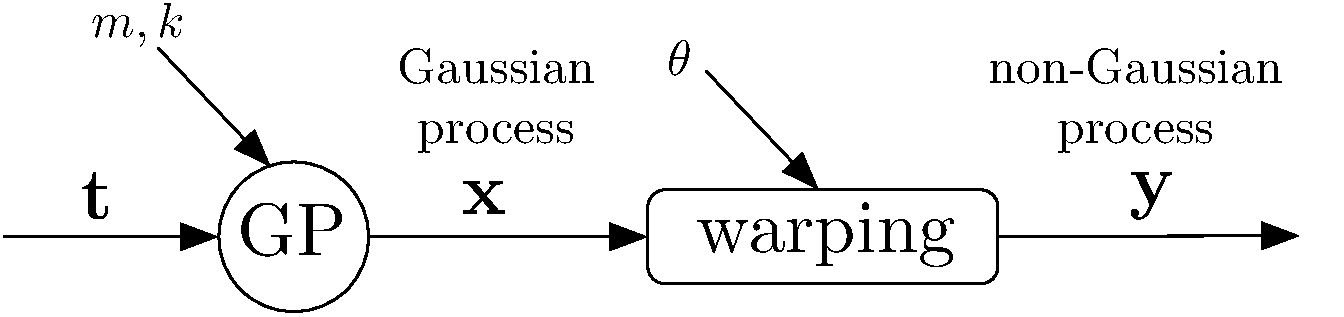
\includegraphics[width=0.6\textwidth]{wgp}
	\caption{Estructura general de los procesos gaussianos deformados, donde se transforma de manera no lineal un GP para modelar observaciones no gaussianas.}
	\label{fig:wgp}
\end{figure}

Para modelar datos no gaussianos y mantener el uso de las ventajas de los modelos gaussianos, uno puede transformar los datos observados \(\bfy \in \calY^N\) vía una biyección no lineal y diferenciable \(\varphi : \calY \to \calX\), llamada \emph{deformación}, tal que \(\bfx = \Phi(\bfy) = [\varphi(y_1), \dotsc, \varphi(y_N)]^\top\) es \emph{más gaussiano} y puede ser modelado como un GP (ver la Figura \ref{fig:wgp}). Este enfoque es estándar en estadística, donde es usual escoger como función a \(\varphi(y) = \log(y)\), en donde se supone implícitamente que el proceso observado tiene marginales log-normales, así que el fenómeno modelado toma valores positivos.

Como la transformación \(\Phi\) es diagonal desde un punto de vista coordenada a coordenada, las distribuciones transformadas satisfacen las condiciones del Teorema de Consistencia de Kolmogorov \cite{tao2011introduction} (introducido en la sección \ref{sec stochastic process}). Dicho modelo generativo es un proceso no gaussiano llamado proceso gaussiano deformado \cite{snelson2004warped}. En la sección \ref{sec:marginaltransport} demostraremos esta proposición de forma más general, así que la consideraremos como cierta por el resto de este capítulo.

Nuestro objetivo es construir una nueva deformación para procesos gaussianos que herede la expresividad de las estructuras más profundas, pero que a la vez requiera aproximaciones numéricas mínimas para poder predecir. Esto se logrará al construir deformaciones que tengan inversas conocidas y con fórmula cerrada.

\section{El Teorema del Cambio de Variables}

\comment{este va aca o en el marco teorico??}
Una manera estándar de abordar el modelamiento de observaciones no gaussianas es transformar los datos usando funciones como el logaritmo \cite{boxcox} o la tangente hiperbólica \cite{johnsonsu}, de forma tal que los datos transformados se distribuyan de forma normal (o estén cerca de hacerlo). Esta transformación resulta en un cambio de la medida de probabilidad \cite{tao2011introduction}, en donde la distribución de la variable transformada, dada la transformación, se conoce explícitamente. Sin embargo, usualmente este resultado y sus implicancias teóricas en la construcción de modelos no gaussianos expresivos son ignorados. Presentamos formalmente el cambio de medida de probabilidad que resulta de transformar una variable aleatoria vía el siguiente teorema, para luego estudiar el caso gaussiano.

\begin{theorem}[Cambio de Variables Probabilístico \cite{hogg1995introduction}]
	\label{thm:CoV}
	Sea \(\bfx \in \calX \subseteq \reals^{n}\) un vector aleatorio con una función de densidad de probabilidad dada por \(p_{\bfx}(\bfx)\), y sea \(\bfy \in \calY \subseteq \reals^n\) un vector aleatorio tal que \(\varphi(\bfy) = \mathbf{x}\), en donde la función \(\varphi : \calY \to \calX\) es biyectiva, de clase \(\calC^{1}\), y \(\vert \nabla \varphi(\bfy) \vert > 0\) para todo \(\bfy \in \calY\). Entonces, la función de densidad de probabilidad \(p_\bfy\) inducida en \(\calY\) está dada por
	\begin{equation*}
		p_{\bfy}(\bfy) = p_{\bfx}(\varphi(\bfy)) \vert \nabla \varphi(\bfy)\vert,
	\end{equation*}
	donde \(\nabla \varphi\) denota al jacobiano de \(\varphi\), y \(\vert \cdot \vert\) denota a la función determinante.
\end{theorem}

Diremos que \(\bfx = [x_{1}, \dotsc, x_{n}]^\top\) son las variables \emph{basales} y que \(\bfy = [y_{1}, \dotsc, y_{n}]^\top\) son las variables \emph{transformadas}. El teorema de cambio de variables nos da una metodología para expresar la función de densidad de probabilidad (f.d.p.) de las variables transformadas en términos de (a) la f.d.p. de las variables basales y (ii) la transformación aplicada.

Como nuestro objetivo es usar el teorema de cambio de variables para construir modelos no gaussianos que sean manejables, consideremos un vector aleatorio normal multivariado \(\bfx \in \reals^n\) con media \(\mu_{\bfx}\) y covarianza \(\Sigma_{\bfx}\), denotado \(\bfx \sim \calN(\mu_{\bfx}, \Sigma_{\bfx})\), y, además, un mapeo coordenada a coordenada\footnote{Para simplificar la notación, denotaremos a los mapeos vectoriales o escalares por \(\varphi\) indistintamente.} desde el espacio transformado al espacio basal dado por
\begin{equation*}
	\bfy \mapsto \bfx = \varphi(\bfy) = [\varphi(y_{1}), \dotsc, \varphi(y_{n})]^\top.
\end{equation*}
Notemos que el jacobiano de \(\varphi(\bfy)\) es diagonal y, por ende, podemos factorizar su determinante como
\begin{equation*}
	\vert \nabla \varphi(\bfy) \vert = \prod_{i=1}^{n} \dv{\varphi(y_{i})}{y} > 0.
\end{equation*}
En este contexto, podemos obtener explícitamente la f.d.p. de \(\bfy = [y_1, \dotsc, y_N]^\top\) usando el teorema \ref{thm:CoV}, y tiene la forma
\begin{equation*}
	p(\bfy) = \prod_{i=1}^{n} \dv{\varphi(y_{i})}{y} \calN(\varphi(\bfy) \mid \mu_{\bfx}, \Sigma_{\bfx}),
\end{equation*}
en donde la función \(\varphi\) es afín si y solo si la distribución \(p(\bfy)\) es gaussiana. Cabe destacar que la distribución \(p(\bfy)\) en general no es gaussiana, pero está parametrizada por la media basal \(\mu_{\bfx}\), la varianza basal \(\Sigma_{\bfx}\) y la transformación\(\varphi\).

También podemos usar el teorema \ref{thm:CoV} para calcular las densidades condicionales de vectores aleatorios gaussianos transformados: para dos vectores conjuntamente gaussianos \(\bfx, \bfx'\) con densidades condicionales \(p(\bfx \mid \bfx') = \calN(\mu_{\bfx \mid \bfx'}, \Sigma_{\bfx \mid \bfx'})\), y un par de vectores \(\bfy, \bfy'\) tales que \(\bfx = \varphi(\bfy)\) y \(\bfx' = \varphi(\bfy')\), la densidad condicional \(p(\bfy \mid \bfy')\) está dada por
\begin{align*}
	p(\bfy \mid \bfy')			&= \prod_{i=1}^{n} \dv{\varphi(y_{i})}{y} \calN(\varphi(\bfy) \mid \mu_{\bfx \mid \bfx'}, \Sigma_{\bfx \mid \bfx'})\\
	\mu_{\bfx \mid \bfx'}		&= \mu_{\bfx} + \Sigma_{\bfx \bfx'} \Sigma_{\bfx' \bfx'}^{-1} (\varphi(\bfy') - \mu_{\bfx'})\\
	\Sigma_{\bfx \mid \bfx'}	&= \Sigma_{\bfx \bfx} - \Sigma_{\bfx \bfx'} \Sigma_{\bfx' \bfx'}^{-1} \Sigma_{\bfx' \bfx},
\end{align*}
donde recordemos que \(\Sigma_{\bfx \bfx'}\) denota la covarianza entre \(\bfx\) y \(\bfx'\), y \(\mu_\bfx\) denota la media marginal de \(\bfx\).

Observemos que la densidad posterior del elemento transformado \(p(\bfy \mid \bfy')\) pertenece a la misma familia que la densidad incondicional \(p(\bfy)\). Esta propiedad de cerradura al tomar condicionales se hereda de la f.d.p. gaussiana base, y se preserva al aplicar la transformación por coordenada \(\varphi\). Más aún, la distribución multivariada no gaussiana \(p(\bfy)\) también es cerrada bajo marginalización y permutación, porque (de nuevo) \(\varphi\) se define por coordenada.

Por lo tanto, podemos construir un proceso no gaussiano al \emph{transformar} (o \emph{deformar}) un GP de la siguiente forma: (i) escogemos un GP base \(x\) y una transformación por coordenada \(\varphi\), (ii) calculamos las densidades marginales finito-dimensionales de \(y\) sujeto a que \(x = \varphi(y)\) usando el teorema de cambio de variables, y (iii) aplicamos el teorema de consistencia de Kolmogorov \cite{tao2011introduction}. Esta construcción garantiza la existencia de tales procesos no gaussianos con hiperparámetros conocidos: la media y la covarianza del GP base, y la transformación \(\varphi\).

\section{Procesos Gaussianos Deformados}
\label{sec:wgp}

Los procesos gaussianos deformados (WGP por sus siglas en inglés) \cite{snelson2004warped} siguen la misma base lógica explicada en la sección anterior. Un WGP considera un GP con media cero y una función de covarianza exponencial cuadrática (SE), así como una transformación por coordenada paramétrica monótona (por ende, invertible).

La transformación \(\varphi : \reals \to \reals\) considerada en \cite{snelson2004warped} está dada por
\begin{equation}
	\label{eq:wgp}
	\varphi (y) = y + \sum_{j=1}^{d} a_{j} \tanh(b_{j}(y + c_{j})),
\end{equation}
donde \(a_{j}, b_{j} \geq 0\) para \(j = 1, \dotsc, d\). La mezcla de las funciones de identidad y la tangente hiperbólica en la ecuación \eqref{eq:wgp} actúa como una deformación paramétrica de la función identidad, lo que significa que el WGP no permite las transformaciones estándar, como el logaritmo. Notemos que, dado que \(\varphi(y)\) en la ecuación \eqref{eq:wgp} es una suma de términos monótonos, su inversa existe. Sin embargo, como esta inversa no se conoce explícitamente, calcular el WGP posterior predictivo requiere aproximar \(\varphi^{-1}\) usando, por ejemplo, el método de Newton-Raphson (NRM) \cite{atkinson2008introduction}. Este procedimiento iterativo requiere varias evaluaciones tanto de \(\varphi\) como de \(\dv*{\varphi}{y}\), lo que incrementa su complejidad computacional sumado a que el método es sensible a la condición inicial. En la práctica, el uso de NRM es el cuello de botella computacional de los WGP: el modelo original propuesto en \cite{snelson2004warped} consideró un enfoque NRM ingenuo que resultó en que la inferencia fue de uno o dos órdenes de magnitud más cara comparada a un GP estándar. Para el tema de la eficiencia computacional, la implementación de \cite{snelson2004warped} consideró un método de bisección para encontrar condiciones iniciales apropiadas para el NRM. Hacemos énfasis en que, a pesar de que la implementación del WGP puede ser más eficiente si es que se usan herramientas numéricas sofisticadas para aproximar funciones inversas, como por ejemplo entrenar un modelo sustituto que usa \emph{splines} o redes neuronales para la inversa, un WGP siempre requiere aproximaciones numéricas cuando se realizan predicciones, debido a que no tenemos una expresión explícita para la inversa de una suma de tangentes hiperbólicas. En \cite{wilson2010copula} los autores proponen una función de deformación alternativa:
\begin{equation*}
	\varphi(x) = \sum_{j=1}^{d} a_{j}\log\big[ 1 + \exp[b_{j}(x + c_{j})]\big],
\end{equation*}
donde \(a_{j}, b_{j} \geq 0\) para \(j=1, \dotsc, d\). Sin embargo, esta deformación hereda los mismos problemas descritos arriba. Por otro lado, el modelo propuesto en la sección \ref{sub:model_description} no sufre este inconveniente.

\subsection{Procesos Gaussianos Deformados Bayesianos}

Una versión no paramétrica del WGP es el WGP bayesiano \cite{bayesianwarped12}, denotado BWGP, que modela a la transformación en sí como un GP con la función identidad como la media. Esta transformación \(phi\) en el BWGP corresponde a la inversa de la transformación \(\varphi\) en el WGP y se puede expresar como
\begin{equation*}
	y(t) = \phi(x(t)) + \varepsilon_{t},
\end{equation*}
donde \(\varepsilon_{t} \sim \calN(0, \sigma^{2})\) y tanto \(x\) como \(\phi\) son GP, es decir
\begin{align*}
	x(t)	&\sim \GP(m(t), k(t, \bar{t}))\\
	\phi(f)	&\sim \GP(f, c(f, \bar{f})),
\end{align*}
donde \(f\) denota a la función de entrada de la deformación \(\phi\) y \(c\) es su kernel de covarianza. Más aún, en \cite{damianou2013deep} se propone una versión profunda del BWGP, con nombre GP Profundo (DGP por sus siglas en inglés, \emph{Deep GP}), en donde la función de deformación es una composición de múltiples GP.

Los DGP, que fueron propuestos principalmente como una extensión de los modelo de variable latente con procesos gaussianos (GP-LVM) \cite{titsias2010bayesian}, que, a su vez, son redes basadas en mapeos de procesos gaussianos, se enfocan en problemas no supervisados (con valores de entrada ocultos y no observados) sobre descubrir estructuras en datos con alta dimensión \cite{lawrence2004gaussian, li2016review, damianou2016variational}. Sin embargo, al reemplazar las entradas latentes con entradas observadas, un modelo de una capa oculta coincide con el BWGP, así que un DGP para regresión también es una generalización de los BWGP \cite{damianou2015deep}. Los DGP son básicamente un GP que alimenta a otro GP, así que son modelos flexibles que pueden capturar funciones altamente no lineales para conjuntos de datos complejos. No obstante, la estructura de red de un DGP hace que realizar inferencia sea computacionalmente cara; incluso las capas internas poseen una patología \cite{duvenaud2014avoiding}. Para usar DGP en escenarios de regresión, algunos autores proponen realizar inferencia usando aproximaciones variacionales \cite{bui2016deep, salimbeni2017doubly} o muestreos secuenciales \cite{wang2016sequential}. Finalmente, los DGP pierden su interpretabilidad, por lo que, como en otros modelos profundos, es difícil entender las propiedades de cada capa y componente.

El entrenamiento y la inferencia no son tratables tanto en BWGP como en DGP; por ende, ambos métodos dependen en enfoques variacionales para realizar inferencia usando una representación \emph{sparse} \cite{titsias2009variational}. Debido a la complejidad computacional considerable, hacer comparaciones del método propuesto contra BWGP y WGP están fuera del alcance de este capítulo, pues nos enfocamos en funciones de deformación expresivas que tengan fórmulas cerradas computacionalmente eficientes para poder entrenar y predecir. Por consiguiente, la validación experimental del método propuesto se realizará solo contra los WGP \cite{snelson2004warped}.

\section{Una Deformación Novedosa para WGP}
\label{sec:novelWGP}
Inspirados por las arquitecturas profundas, proponemos un modelo generativo para procesos no gaussianos vía la transformación de un GP latente por una composición de \emph{funciones elementales} \(\varphi_i\), teniendo dos objetivos en mente. El primero es que la clase de transformaciones tiene que ser lo suficientemente general para poder replicar a una amplia clase de datos usando pocos parámetros para evitar sobreajustes, mientras que el segundo es que las aproximaciones necesarias para aprender y hacer inferencia deben ser mínimas, para mantener la precisión numérica alta y la complejidad computacional baja.

\subsection{Descripción del Modelo}
\label{sub:model_description}

Consideremos una familia de funciones paramétricas \(\{\varphi_i\}_{i=1}^d\), con \(d \in \naturals\), diferenciables, invertibles y cuya inversa tiene fórmula cerrada. De ahora en adelante las llamaremos \emph{funciones elementales}. Entonces, podemos construir funciones de deformación \(\varphi\) como la composición de tales funciones elementales, es decir,
\begin{equation*}
	\varphi = \varphi_d \circ \varphi_{d-1} \circ \dotsb \circ \varphi_{2} \circ \varphi_1.
\end{equation*}
La motivación de esta construcción es el hecho de que la inversa y las derivadas de las composiciones de funciones dependen de las inversas y las derivadas de las funciones que la componen. Por ejemplo, para una composición de dos funciones elementales \(\varphi(y) = \varphi_{2}(\varphi_{1}(y)) = x\), la inversa y la derivada están dadas respectivamente por:
\begin{align*}
	\varphi^{-1}(x)		&= \varphi_{1}^{-1}(\varphi_{2}^{-1}(x)) \\
	\dv{\varphi(y)}{y}	&= \dv{\varphi_{2}(\varphi_{1}(y))}{y} \dv{\varphi_{1}(y)}{y}.
\end{align*}
Notemos que esta clase de funciones de deformación va un paso más allá comparado a los WGP: un WGP requiere de la invertibilidad, pero luego requiere de encontrar la inversa numéricamente; por otro lado, la deformación por composición propuesta requiere de la invertibilidad y las inversas con fórmula cerrada, lo que significa que la evaluación de la inversa es directa.

Proponemos a continuación el proceso gaussiano deformado por composiciones (CWGP) dado por \(y(t)\) sujeto a:
\begin{align*}
	\varphi(y(t))	&= x(t),\\
	x(t)			&\sim \GP(m(t), k(t, \bar{t})),\\
	\varphi			&= \varphi_d \circ \dotsb \circ \varphi_2 \circ \varphi_1,
\end{align*}
en donde \(\{\varphi_i\}_{i=1}^d\) son funciones elementales. Adicionalmente, como la inversa de \(\varphi\) es conocida, un CWGP también se puede interpretar como un modelo generativo que transforma \(x(t)\) en \(y(t)\) usando la transformación \(\varphi^{-1}\). En virtud de la claridad notacional, hacemos el énfasis de que \(\varphi\) se define desde el proceso no gaussiano \(y\) hacia el proceso gaussiano \(x\).

Por último, también clarificamos que el modelo descrito arriba difiere radicalmente del concepto de Flujos Normalizadores (NF por sus siglas en inglés, \emph{Normalising Flows}) \cite{tabak2010,tabak2013,rezende2015variational}. Un NF se enfoca en aproximar la densidad posterior de un modelo intratable, mientras que nosotros construimos un modelo generativo no gaussiano directamente.

\subsection{Aprendizaje: robusto, interpretable y eficiente}
\label{sub:sampling}

Aprender bajo un CWGP significa encontrar los hiperparámetros del GP \(x\) (i.e. los parámetros del kernel y la media, denotados \(\theta_x\)) además de los parámetros de la transformación \(\varphi\), denotados \(\theta_\varphi\). Gracias al teorema de cambio de variables, encontrar estos parámetros es tratable, y se puede lograr al minimizar el logaritmo negativo de la verosimilitud marginal (NLL).

Con respecto a la robustez, así como en los GP estándar, los GP deformados están protegidos del sobreajuste, pues parametrizan a una distribución prior sobre funciones directamente, y no a las trayectorias específicas de la función. Recordemos además que la deformación considerada se aplica por componente y está dada por el mismo mapeo a valores escalares para todas las componentes. Por ende, podemos entender la deformación como una parametrización del histograma marginal. en consecuencia, el modelo generativo resultante tiene marginales no gaussianas con cópulas gaussianas, conocido como el \emph{proceso gaussiano con cópulas} \cite{wilson2010copula}, lo que quiere decir, en el sentido amplio de modelar la ley del proceso estocástico, que el modelo propuesto está regularizado por diseño.

Con respecto a la interpretabilidad, la NLL está dada por cuatro términos:
\begin{align}
\label{eq:NLL}
	\mathrm{NLL}	=& -\log p(\bfy \mid \theta_x, \theta_\varphi)\\
					=& \underbrace{\frac{n \log(2\pi)}{2}}_{\text{constante}} + \underbrace{\frac{1}{2}(\varphi(\bfy) - \mu_{\bfx})^{\top} \Sigma_{\bfx \bfx}^{-1} (\varphi(\bfy)-\mu_{\bfx})}_{\text{ajuste a los datos}} \nonumber\\
					&+ \underbrace{\frac{1}{2} \log \lvert \Sigma_{\bfx \bfx} \rvert}_{\substack{\text{complejidad} \\ \text{del kernel}}} - \underbrace{\sum_{i=1}^{n} \log\left( \dv{\varphi(y_{i})}{y} \right)}_{\substack{\text{complejidad} \\ \text{de la deformación}}},
	\nonumber
\end{align}
en donde \(\mu_\bfx\) y \(\Sigma_{\bfx \bfx}\) son la media y la covarianza de \(\bfx = \varphi(\bfy)\).

Similar a los GP estándar, para los cuales la NLL explicita automáticamente la penalidad que se incurre por tener un modelo complejo, los WGP presentan un término relacionado a la complejidad de la deformación. Así, la minimización de la NLL balancea la gaussianidad del GP basal \(x\) vía los tres primeros términos de la ecuación \eqref{eq:NLL} y la regularidad de la deformación vía el término final de la misma ecuación. El primer criterio prioriza soluciones tales que \(\lVert \varphi(\bfy) - \mu_{\bfx} \rVert\) sea pequeño con rexpecto a la norma inducida por \(\Sigma_{\bfx \bfx}^{-1}\), en donde la solución extrema es \(\varphi(\bfy) = \mu_{\bfx}\), una constante para todo \(\bfy\) y \(t\), pues \(\varphi(\bfy) : \bfy \mapsto x\) y \(\mu_{\bfx} : t \mapsto x\). Sin embargo, notemos que el término de la complejidad de la deformación \(\sum_{i=1}^{n} \log(\dv*{\varphi(y_{i})}{y})\) fuerza a que las soluciones \(\varphi(\bfy)\) tengan derivadas grandes (es decir, que crezcan abruptamente), lo que descarta a la solución constante. Estos términos ofrecen una interpretación clara de la función de verosimilitud del WGP: el término que penaliza a la deformación promueve que se preserve la variabilidad de los datos al escoger deformaciones con derivadas grandes, mientras que los otros términos aseguran que esta variabilidad se mantenga lo más gaussiana posible.

Con respecto a complejidad computacional, notemos que minimizar la NLL no requiere la inversa de \(\varphi\), sino que solo los logaritmos de las derivadas, que tienen fórmula cerrada, por lo que el costo de entrenar un CWGP está dominado por la inversión de la matriz: \(O(n^3)\) para \(n\) observaciones. Recordemos que este es el mismo orden de complejidad de entrenar un GP estándar. De forma intuitiva, aprender se logra al transformar las observaciones no gaussianas para luego maximizar la probabilidad (gaussiana) de las muestras transformadas con respecto a los parámetros de (i) la distribución gaussiana y (ii) aquellos de la transformación. Si bien la complejidad de evaluar la NLL de un CWGP es igual a la de un GP estándar, nuestro modelo es más expresivo, por lo que la NLL puede tener más mínimos locales debido a que tiene más parámetros que entrenar. Para más detalles, recomendamos leer \cite{rios2018learning}, en donde se exploran múltiples mínimos locales con optimizaciones basadas en Monte Carlo y libres de derivadas.

\subsection{Inferencia en Fórmula Cerrada}

La inferencia se sigue de un corolario del teorema de cambio de variables que dice que la (medida de) probabilidad de un conjunto \(E\) bajo la densidad de \(\bfy\) es igual a la probabilidad de la imagen de \(E\), \(\varphi(E)\), bajo la densidad de \(\bfx\). Condicionando en los datos observados \(\bfy\), podemos expresar el corolario como sigue:
\begin{align*}
	\int_{E} p_{y}(y \mid \bfy) \dd{y} = \int_{\varphi(E)} p_{x}(x \mid \bfy) \dd{x} = \int_{\varphi(E)} p_{x}(x \mid \bfx) \dd{x},
\end{align*}
en donde la primera igualdad se tiene por el teorema \ref{thm:CoV} y la segunda se tiene por la relación determinista \(\bfx = \varphi(\bfy)\). Para elecciones distintas del conjunto \(E\) y usando la transformación inversa explícita \(\varphi^{-1}\), podemos expresar la mediana de \(y(t)\) y los intervalos de confianza con el percentil \(p\) \textbf{en forma cerrada} como sigue:
\begin{align*}
	\median({y(t)})	&= \varphi^{-1}\bigl(\median({x(t)})\bigr) = \varphi^{-1}\left(m(t)\right)\\
	I_{y(t)}^p		&= \bigl[\phi^{-1}(m(t) - z_{p}\sigma(t)), \phi^{-1}(m(t) + z_{p}\sigma(t))\bigr],
\end{align*} 
en donde \(\sigma(t) = \sqrt{k(t, t)}\) es la desviación estándar del GP basal, \(z_{p}\) es el cuantil \(p\) de una gaussiana estándar (p. ej. \(z_{0.975} \approx 1.96\)), y usamos el hecho de que para una gaussiana \(\median(x) = \mean(x)\).

Muestrear el proceso no gaussiano también es directo: solo se requiere simular una realización del GP y luego aplicar la inversa de la transformación por coordenada, es decir,
\begin{align*}
	x(\bft)	&\sim \GP(m(\bft), k(\bft, \bft))\\
	y(\bft)	&= \varphi^{-1}(x(\bft)).
\end{align*}

\subsection{Análisis de Complejidad de la Inferencia}

Fiándonos una vez más del teorema de cambio de variables, la esperanza de una función medible \(h : \calY \to \reals\) bajo una ley no gaussiana \(p(\bfy)\) está dada por
\begin{align*}
	\mean_{\bfy}[h(\bfy)] = \mean_{\bfx} \bigl[h\bigl(\varphi^{-1}(\bfx)\bigr)\bigr].
\end{align*}
Además, como la distribución de \(\bfx\) es gaussiana, podemos calcular de forma eficiente la integral de arriba de forma numérica, usando la cuadratura de Gauss-Hermite \cite{gausshermite64}, para la cual las aproximaciones de \(k\) puntos son exactas cuando el integrando \(h \circ \varphi^{-1}\) es un polinomio de orden \(2k-1\). Escogiendo \(h(y)=y\), tenemos que la aproximación de la media de \(y\) está dada por
\begin{align}
	\label{eq:exp_CWGP}
	\mean_{y}[y]	&= \int \varphi^{-1}(x) p_{x}(x) \dd{x} \nonumber\\
					&\approx \frac{1}{\sqrt{\pi}} \sum_{i=1}^{k} w_{i} \varphi^{-1}\left(\sqrt{2}\sigma_{x} x_{i} + m_{x} \right),
\end{align}
en donde los pesos \(\{w_{i}\}_{i=1}^k\) y las posiciones \(\{x_{i}\}_{i=1}^k\) están dados por la cuadratura de Gauss-Hermite\cite{gausshermite64}. 

Por último, observemos que es necesario evaluar \(\varphi^{-1}\) para calcular esperanzas, la mediana y los intervalos de confianza del modelo no gaussiano. Ya que en un CWGP conocemos \(\varphi^{-1}\), el costo de evaluarla es \(O(d)\), donde \(d\) es el número de funciones elementales de \(\varphi\). En consecuencia, el costo de evaluar \(\mean_{y}[y]\) en la ecuación \eqref{eq:exp_CWGP} usando la cuadratura de Gauss-Hermite de \(k\) puntos es \(O(kd)\) en un CWGP. En cambio, un WGP aproxima a \(\varphi^{-1}\) usando el método de Newton-Raphson (NRM) \cite{atkinson2008introduction} (aplicando el método de la bisección para encontrar el punto inicial), lo que significa que el costo de evaluar \(\mean_{y}[y]\) para un WGP es \(O(kdt)\), donde \(t\) es el número de iteraciones del NRM y de la bisección. En la práctica, la expresión explícita de \(\varphi^{-1}\) es clave en términos computacionales: aún cuando se usen métodos numéricos eficientes, un WGP siempre requiere aproximaciones numéricas de \(\varphi^{-1}\), mientras que un CWGP no, y puede evaluar \(\varphi^{-1}\) directamente.

\section{Transformaciones Elementales}
\label{sec:transformations}

Acompañando a los CWGP de la sección previa, presentamos un conjunto de transformaciones elementales con inversa y derivada explícitas, a ser usadas como las funciones más fundamentales de una transformación por composición de un CWGP. Más aún, para mantener la consistencia con el teorema \ref{thm:CoV}, presentamos las transformaciones desde el proceso no gaussiano \(y\) hacia el GP \(x\). La tabla \ref{tab:table_transformations} resume estas transformaciones, junto a sus inversas y derivadas, y la figura \ref{fig:tgp_processes} muestra dos familias distintas de transformaciones, junto a sus densidades marginales inducidas y trayectorias muestreadas.

\begin{table*}[h]
	\centering
	\label{tab:table_transformations}
	\begin{tabular}{l|ccc}
		%\toprule
		Función		& \(\varphi(y)\)												& \(\dv{\varphi(y)}{y}\)								& \(\varphi^{-1}(x)\) \\
		\hline
		%\midrule
		Afín		& \(a + by\)													& \(b\)													& \(\frac{x-a}{b}\)\\
		Logaritmo	& \(\log(y)\)													& \(y^{-1}\)											& \(\exp(x)\) \\
		Asinh		& \(a + b \asinh\left(\frac{y - c}{d}\right)\)					& \(\frac{b}{\sqrt{d^2 + (y-c)^{2}}}\)					& \(c + d\sinh\left(\frac{x - a}{b}\right)\) \\
		Box-Cox		& \(\frac{\sgn(y) \lvert y\rvert^{\lambda} - 1}{\lambda}\)		& \(\lvert y\rvert^{\lambda - 1}\)						& \(\sgn(\lambda x + 1) \lvert \lambda x + 1 \rvert^{\frac{1}{\lambda}}\) \\
		Sinh-Asinh	& \(\sinh(b\asinh(y) - a)\)										& \(\frac{b\cosh(b\asinh(y) - a)}{\sqrt{1 + y^{2}}}\)	& \(\sinh\left(\frac{1}{b} (\asinh(x) + a)\right)\) \\
		%\bottomrule
	\end{tabular}
	\caption{Transformaciones elementales: formas funcionales con derivadas e inversas.}
\end{table*}

\begin{figure*}[h]
	\centering
	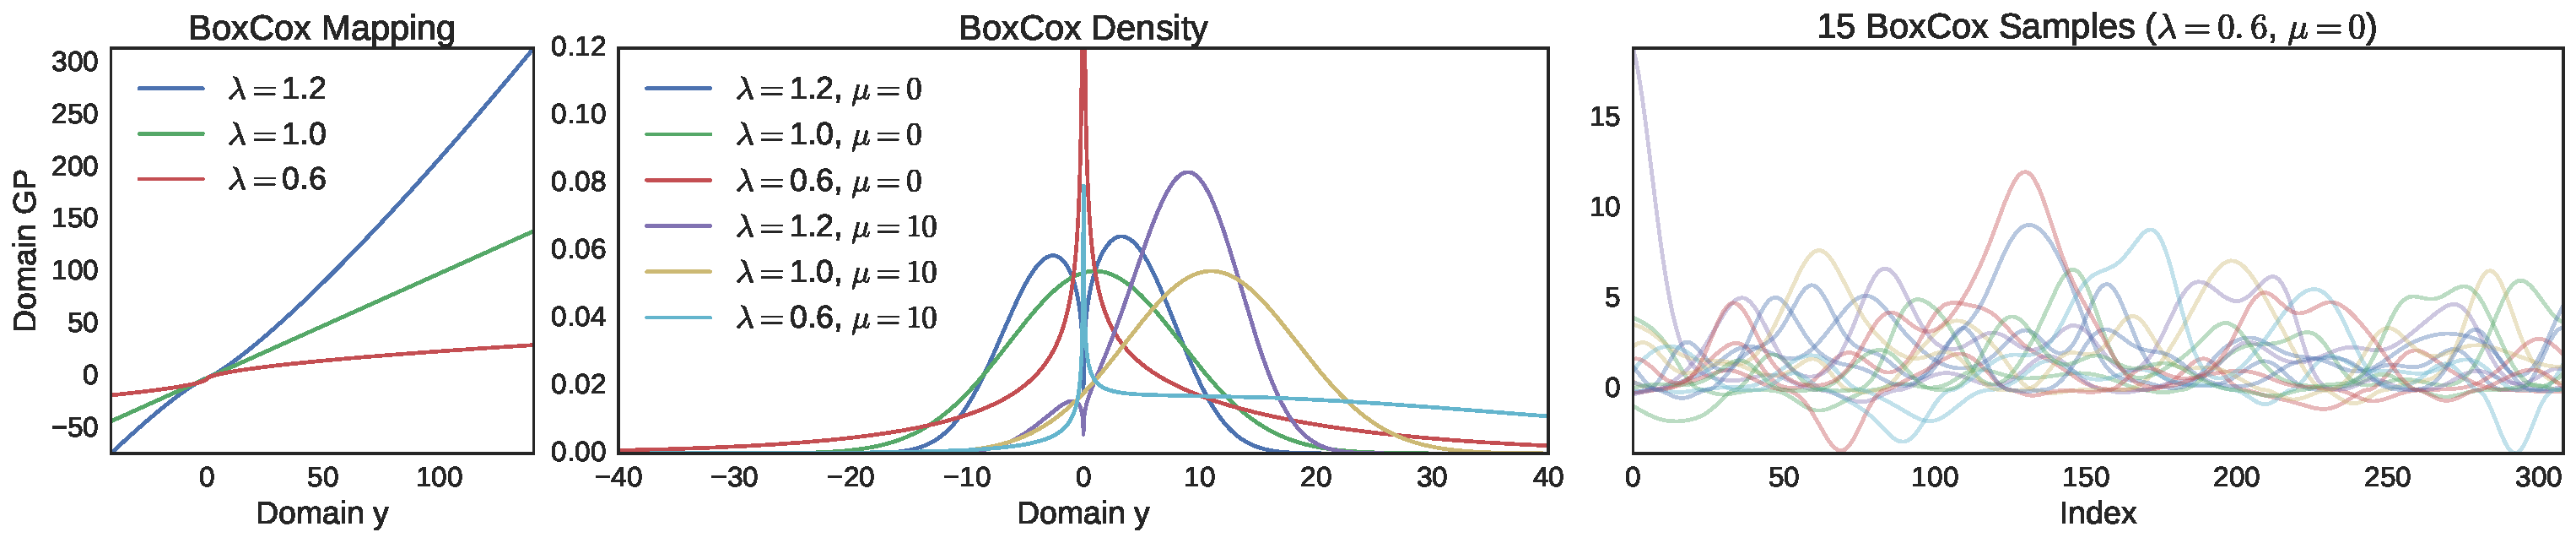
\includegraphics[width=1.0\textwidth]{boxcox_density_samples}\\
	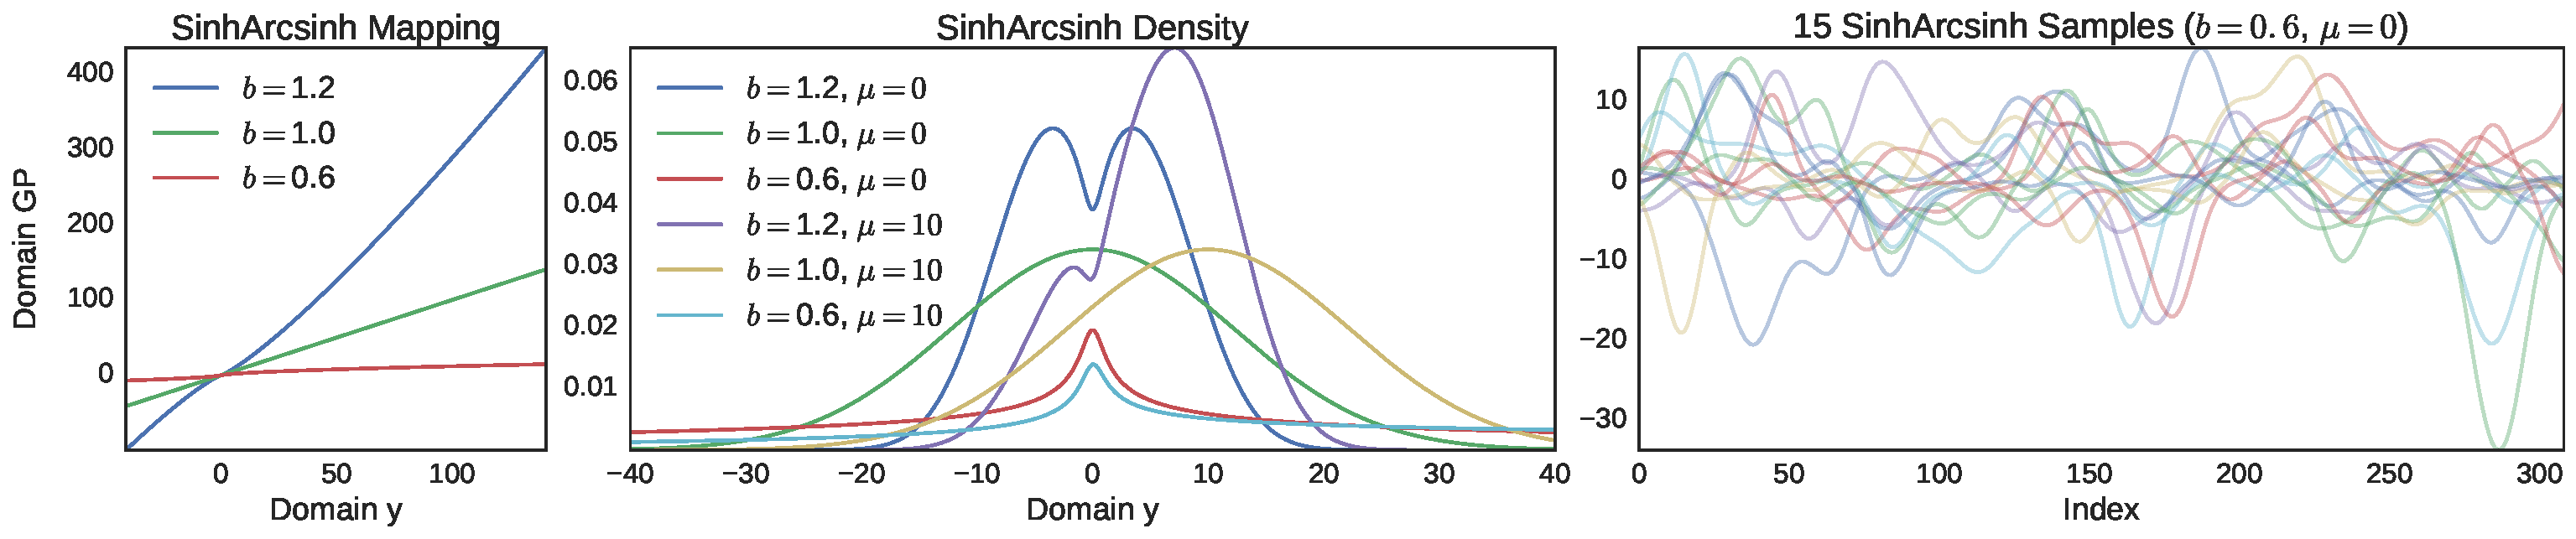
\includegraphics[width=1.0\textwidth]{sinharcsinh_density_samples} %scale=0.29, clip,trim=30 0 0 0
	\caption{Transformaciones elementales Box-Cox y Sinh-Asinh propuestas. Para todos los gráficos, \(\mu\) denota la media del GP basal \(x\). Arriba: la transformación de Box-Cox en la ecuación \eqref{eq:box-cox-trans}. Abajo: la transformación Sinh-Asinh en la ecuación \eqref{eq:sinharcsinh-trans}. Izquierda: las transformaciones. Centro: las densidades marginales inducidas. Derecha: muestras del GP deformado.}
	\label{fig:tgp_processes}
	%\vspace{-1em}
\end{figure*}

\subsection{Transformación Afín}

La transformación afín está dada por
\begin{equation}
	\label{eq:affine-trans}
	\varphi_{\text{afín}}(y) = a + by,
\end{equation}
para \(a, b \in \reals\), y se llama \emph{desplazamiento} (\emph{shift} en inglés) cuando \(b=1\) y \emph{escala} cuando \(a=0\). La transformación afín no proporcional ninguna capacidad mejorada para modelar por sobre los GP estándar, pues un GP transformado por \(\varphi_{\text{afín}}\) sigue siendo un GP con la media desplazada la varianza escalada. sin embargo, la deformación afín puede ser compuesta con otras funciones elementales para producir transformaciones expresivas.

\subsection{Transformaciones de Box-Cox}
\label{sec:BC_trans}
Una estrategia estándar en estadística para transformar observaciones no gaussianas positivas en unas \emph{parecidas a gaussianas} es aplicar la función logaritmo \(\varphi_{\log}(y) = \log(y)\). Este es el caso de procesos estocásticos con valores positivos y de colas pesadas \cite{aitchison1976lognormal}. Notemos que con la transformación logarítmica tanto la media \(m_x\) y la varianza \(\sigma_x^2\) del GP original \(x\) afectan a todos los momentos delproceso transformado \(y\). De forma explícita, el \(n\)-ésimo momento de \(y\) está dado por
\begin{equation}
	\mean_{y}[y^{n}] = \exp \bigl(nm_{x} + \tfrac{1}{2}n^{2} \sigma_{x}\bigr),
\end{equation}
lo que significa que una distribución con cola pesada para \(y\) se obtiene solo mediante la modificación de la media y la varianza del proceso original \(x\).

Una generalización de la transformación logarítmica es la transformación de Box-Cox \cite{boxcox,sakia1992box}, una función de potencias de un parámetro dada por
\begin{equation}
	\label{eq:box-cox-trans}
	\varphi_{\lambda}(y) = \frac{\sgn(y) \lvert y \rvert^{\lambda} - 1}{\lambda},
\end{equation}
donde \(\lambda \in \reals^{+}_{0}\). La función \(\varphi_{\lambda}\) se vuelve una de potencias para \(\lambda >0\), una transformación afín cuando \(\lambda = 1\), y la transformación logarítmica cuando \(\lambda = 0\), pues \(\varphi_{\lambda} \to \log(y)\) cuando \(\lambda \to 0\).

La transformación de Box-Cox tiene dos propiedades útiles. La primera es que su moda es \cite{powernormal}
\begin{align*}
	\mode(y) = \left[\frac{1}{2} \left(1 + \lambda m_x + \sqrt{(1 + \lambda m_x)^{2} + 4 \sigma_x^2 \lambda (\lambda - 1)}\right)\right]^{\frac{1}{\lambda}},
\end{align*}
donde \(m_x\) y \(\sigma_x^2\) son la media y la varianza del GP \(x\) respectivamente. Esta fórmula es particularmente útil para distribuciones asimétricas, donde es usual estimar la moda, no así la media o la mediana. La segunda propiedad es que el cálculo de momentos usando métodos numéricos, como la cuadratura de Gauss-Hermite \cite{gausshermite64}, se puede realizar con una precisión alta debido a la naturaleza polinomial de la transformación de Box-Cox. La figura \ref{fig:tgp_processes} (arriba) muestra diferentes transformaciones de Box-Cox con sus densidades marginales inducidas.

\subsection{Transformaciones hiperbólicas}
La distribución que resulta de tomar una variable aleatoria distribuida como \(\calN(0, 1)\) y aplicarle la transformación del seno hiperbólico inverso
\begin{align}
	\label{eq:arcsinh-trans}
	\varphi_{\asinh}(y) = a + b \asinh\left(\frac{y - c}{d}\right),
\end{align}
donde \(a, c \in \reals\) y \(b, d \in \reals^{+}\), se conoce como la distribución SU de Johnson \cite{johnsonsu} y tiene expresiones cerradas para la media y la varianza, dadas respectivamente por
\begin{align*}
	\mu_{\mathrm{SU}}			&= c - d \exp\left(\frac{b^{-2}}{2}\right) \sinh\Bigl(\frac{a}{b}\Bigr)\\
	\sigma_{\mathrm{SU}}^{2}	&= \frac{d^{2}}{2} \bigl(\exp\left(b^{-2}\right) - 1\bigr) \left[\exp\left(b^{-2}\right) \cosh\left(\frac{2a}{b}\right) + 1\right],
\end{align*}
y también para la asimetría y la curtosis \cite{johnsonsu}.

Otra transformación basada en fuciones hiperbólicas es la Sinh-Asinh \cite{Sinharcsinh}, en donde las funciones \(\asinh\), afín, y \(\sinh\) se componen como sigue:
\begin{equation}
	\label{eq:sinharcsinh-trans}
	\varphi_{\text{Sinh-Asinh}}(y) = \sinh(b\asinh(y) - a),
\end{equation}
en donde \(a, b \in \reals\). Esta distribución tiene expresiones explícitas para todos los momentos de \(y\), usando la función de Bessel modificada, e induce una distribución en donde los tercer y cuarto momentos pueden ser controlas a través de los parámetros \(a\) y \(b\). Esta distribución es simétrica si \(a = 0\), asimétrica positiva (resp. negativa) si \(a > 0\) (resp. \(a < 0\)), mesocúrtica si \(b = 1\), y leptocúrtica (resp. platicúrtica) si \(b > 1\) (resp. \(b < 1\)). Adicionalmente, la distribución cumple que \(0 < \lvert \mode(y) \rvert < \sinh(\lvert a \rvert / b)\) y \(\sgn(\mode(y)) = \sgn(a)\).

La figura \ref{fig:tgp_processes} (abajo) muestra transformaciones Sinh-Asinh con las marginales inducidas y muestras con un parámetro de asimetría \(a = 0\) y diferentes valores del parámetro de curtosis \(b\). Notemos que la media del GP basal, \(\mu\), también puede cambiar la asimetría de la distribución marginal inducida.

\section{¿Cómo Elegir las Transformaciones Elementales?}
\label{sec:choice_trans}

Así como en la gran mayoría de las estructuras profundas, la definición del número de capas y el tipo de neuronas está dada o por expertos o por prueba y error, done la interpretabilidad es una propiedad deseable \cite{representation_NN}. Esta habilidad es necesaria también en el caso cuando se escoge el kernel en máquinas de vectores de soporte o en procesos gaussianos (estudiado en \cite{duvenaud2013structure}). Recordemos que en los modelos de mezcla estándar (como un WGP) el usuario solo define el número de componentes, mientras que dentro del CWGP propuesto uno también necesita elgir los tipos y el orden de los elementos (en nuestro caso, funciones elementales). Esta sección guía la elección de las transformaciones elementales bajo dos escenarios, el primero siendo el caso cuando existe un conocimiento de expertos sobre los datos. En el segundo escenario, es decir, cuando no existe una información a priori de los datos, mostramos que se puede implementar un CWGP al concatenar múltiples instancias de una secuencia particular de funciones elementales (llamadas la \emph{capa Sinh-Asinh-Afín}), y mostramos que esta construcción tiene un rendimiento experimental atractivo. De esta forma, el CWGP puede ser considerado como una «caja negra» en donde, similar a las estructuras profundas, el usuario solo necesita escoger el número de capas. Ilustramos este concepto basado en la NLL (en la sección \ref{sub:sparse_trans}) y a través de un ejemplo de juguete (en la sección \ref{sub:replicating_wgp}), así como su robustez al sobreajustar y a través de datos reales en la sección \ref{sub:sunspots}.

\subsection{Cuando conocimiento previo de los datos está disponible}

Como mencionamos en la sección \ref{sec:BC_trans}, cuando los datos son estrictamente positivos, una práctica estándar es aplicar la transformación logarítmica. Es crítico que si se sabe que los datos tienen una cota inferior desconocida, uno puede componer la transformación logarítmica con la transformación \emph{shift} de la ecuación \eqref{eq:affine-trans} para encontrar el parámetro de \emph{shift} durante el entrenamiento. Encontrar una cota superior sigue un proceso análogo al reemplazar el \emph{shift} por una transformación afín, permitiendo así un escalamiento negativo. En este sentido, componer dos transformaciones afín-logarítmica nos permite encontrar las cotas inferior y superior simultáneamente.

Para relajar aún más la condición estricta de la cota (inferior) de la transformación logarítmica a una más permisiva, podemos reemplazar el logaritmo por la transformación de Box-Cox en la ecuación \eqref{eq:box-cox-trans}, en donde la permisividad de la cota está controlada por el parámetro \(\lambda\). Sumado a esto, si los datos son tales que su rango no está acotado, pero sí tienen una dispersión grande, entonces los datos siguen una distribución de cola pesada. Este fenómeno se puede modelar usando las transformaciones Asinh o Sinh-Asinh de las ecuaciones \eqref{eq:arcsinh-trans} y \eqref{eq:sinharcsinh-trans} respectivamente, pues dichas transformaciones permiten controlar la media y la varianza de la distribución, así como su asimetría y curtosis. Todas estas transformaciones pueden ser compuestas entre ellas para construir distribuciones más complejas, como en el caso de las distribuciones multimodales.

\subsection{Transformaciones compuestas \emph{sparse}}
\label{sub:sparse_trans}

Así como en cualquier modelo que involucre escoger un orden finito (como capas, neuronas, o componentes), se requiere que la adición de más funciones elementales en un CWGP tenga como resultado un desempeño monótonamente creciente. En particular, si uno considera un número innecesariamente grande de transformaciones elementales, es deseable que algunas de ellas \emph{se reviertan} a la función identidad (y así puedan ser removidas). Si, después de entrenar, algunas de las transformaciones se revierten a la identidad, diremos que la transformación compuesta es \emph{sparse}.

Cuando la intuición de las propiedades estadísticas de los datos es escasa, o incluso inexistente, un procedimiento recomendado es añadir de forma secuencial transformaciones que pueden revertirse a la identidad en caso de ser necesario. Notemos que si una transformación no es capaz de mejorar el desempeño y a la vez sí puede revertirse a la identidad, en efecto hará este. Este hecho se puede justificar basándonos en la NLL en la ecuación \eqref{eq:NLL}, en donde el término de ajuste a los datos permanece invariante, y el término de complejidad de la deformación contribuye a una NLL más baja. Sumado a esto, uno siempre puede escoger una distribución prior sobre los parámetros de la deformación para promover más deformaciones que estén cerca de la identidad. Finalmente, recordemos que, de las transformaciones propuestas, la Box-cox, la Sinh-Asinh y la afín pueden revertirse a la identidad, por lo que, bajo un conocimiento limitado sobre las propiedades subyacentes de los datos, recomendamos añadir estas componentes de forma iterativa hasta que el desempeño del modelo alcance una meseta. A continuación implementamos este concepto basados solo en las transformaciones Sinh-Asinh y afín en datos sintéticos.

\subsection{Descubrimiento de estructuras a través de transformaciones compuestas profundas}
\label{sec:experiments}

En los casos en que un conocimiento experto de los datos es escaso, el CWGP propuesto puede implementarse solo al concatenar múltiples instancias de las transformaciones elementales propuestas. Este procedimiento es usual y aceptado ampliamente en arquitecturas profundas generales \cite{bengio2009learning,Goodfellow-et-al-2016,DL_overview}. Para ilustrar esto, definamos primero la composición de las transformaciones Sinh-Asinh y Afín, de las ecuaciones \eqref{eq:arcsinh-trans} y \eqref{eq:affine-trans} respectivamente, llamada la \emph{capa SAL}\footnote{El acrónimo SAL viene de «Sinh-Asinh» y «Afín», done el uso de «L» viene de «lineal». Elegimos esta terminología para ser consistente con la parte experimental en la próxima sección.} dada por
\begin{equation}
	\label{eq:layer}
	l(y) = a + b \sinh(c \arcsinh(y) - d),
\end{equation}
donde \(a, b, c, d \in \reals\) son los únicos cuatro parámetros de la capa. Mostramos a continuación que solo al concatenar capas SAL podemos replicar la deformación «suma de tangentes hiperbólicas» implementada por un WGP \cite{snelson2004warped}, en la ecuación \eqref{eq:wgp}. La razón para evaluar el modelo propuesto en la aproximación del WGP es que se sabe que la suma de tangentes hiperbólicas es \emph{universal}, lo que significa que puede aproximar funciones continuas en cualquier grado de exactitud deseado en un intervalo cerrado.

Con la intención de obtener una comprensión intuitiva sobre la habilidad para modelar del enfoque por composiciones, el primer ejemplo ilustrativo es entrenar una transformación por composición de tres capas SAL, vía mínimos cuadrados, para replicar una mezcla de tres tangentes hiperbólicas. La figura \ref{fig:cwgp_flexible} muestra las transformaciones, derivadas, densidades y distribuciones de la verdad básica (el WGP, en azul) y la aproximación por composición de tres capas SAL (el CWGP, en verde). Notemos la similaridad punto a punto de las deformaciones, y que la masa de probabilidad se concentra alrededor de tres modas comunes en el dominio de \(y\).

\begin{figure}[h]
	\centering
	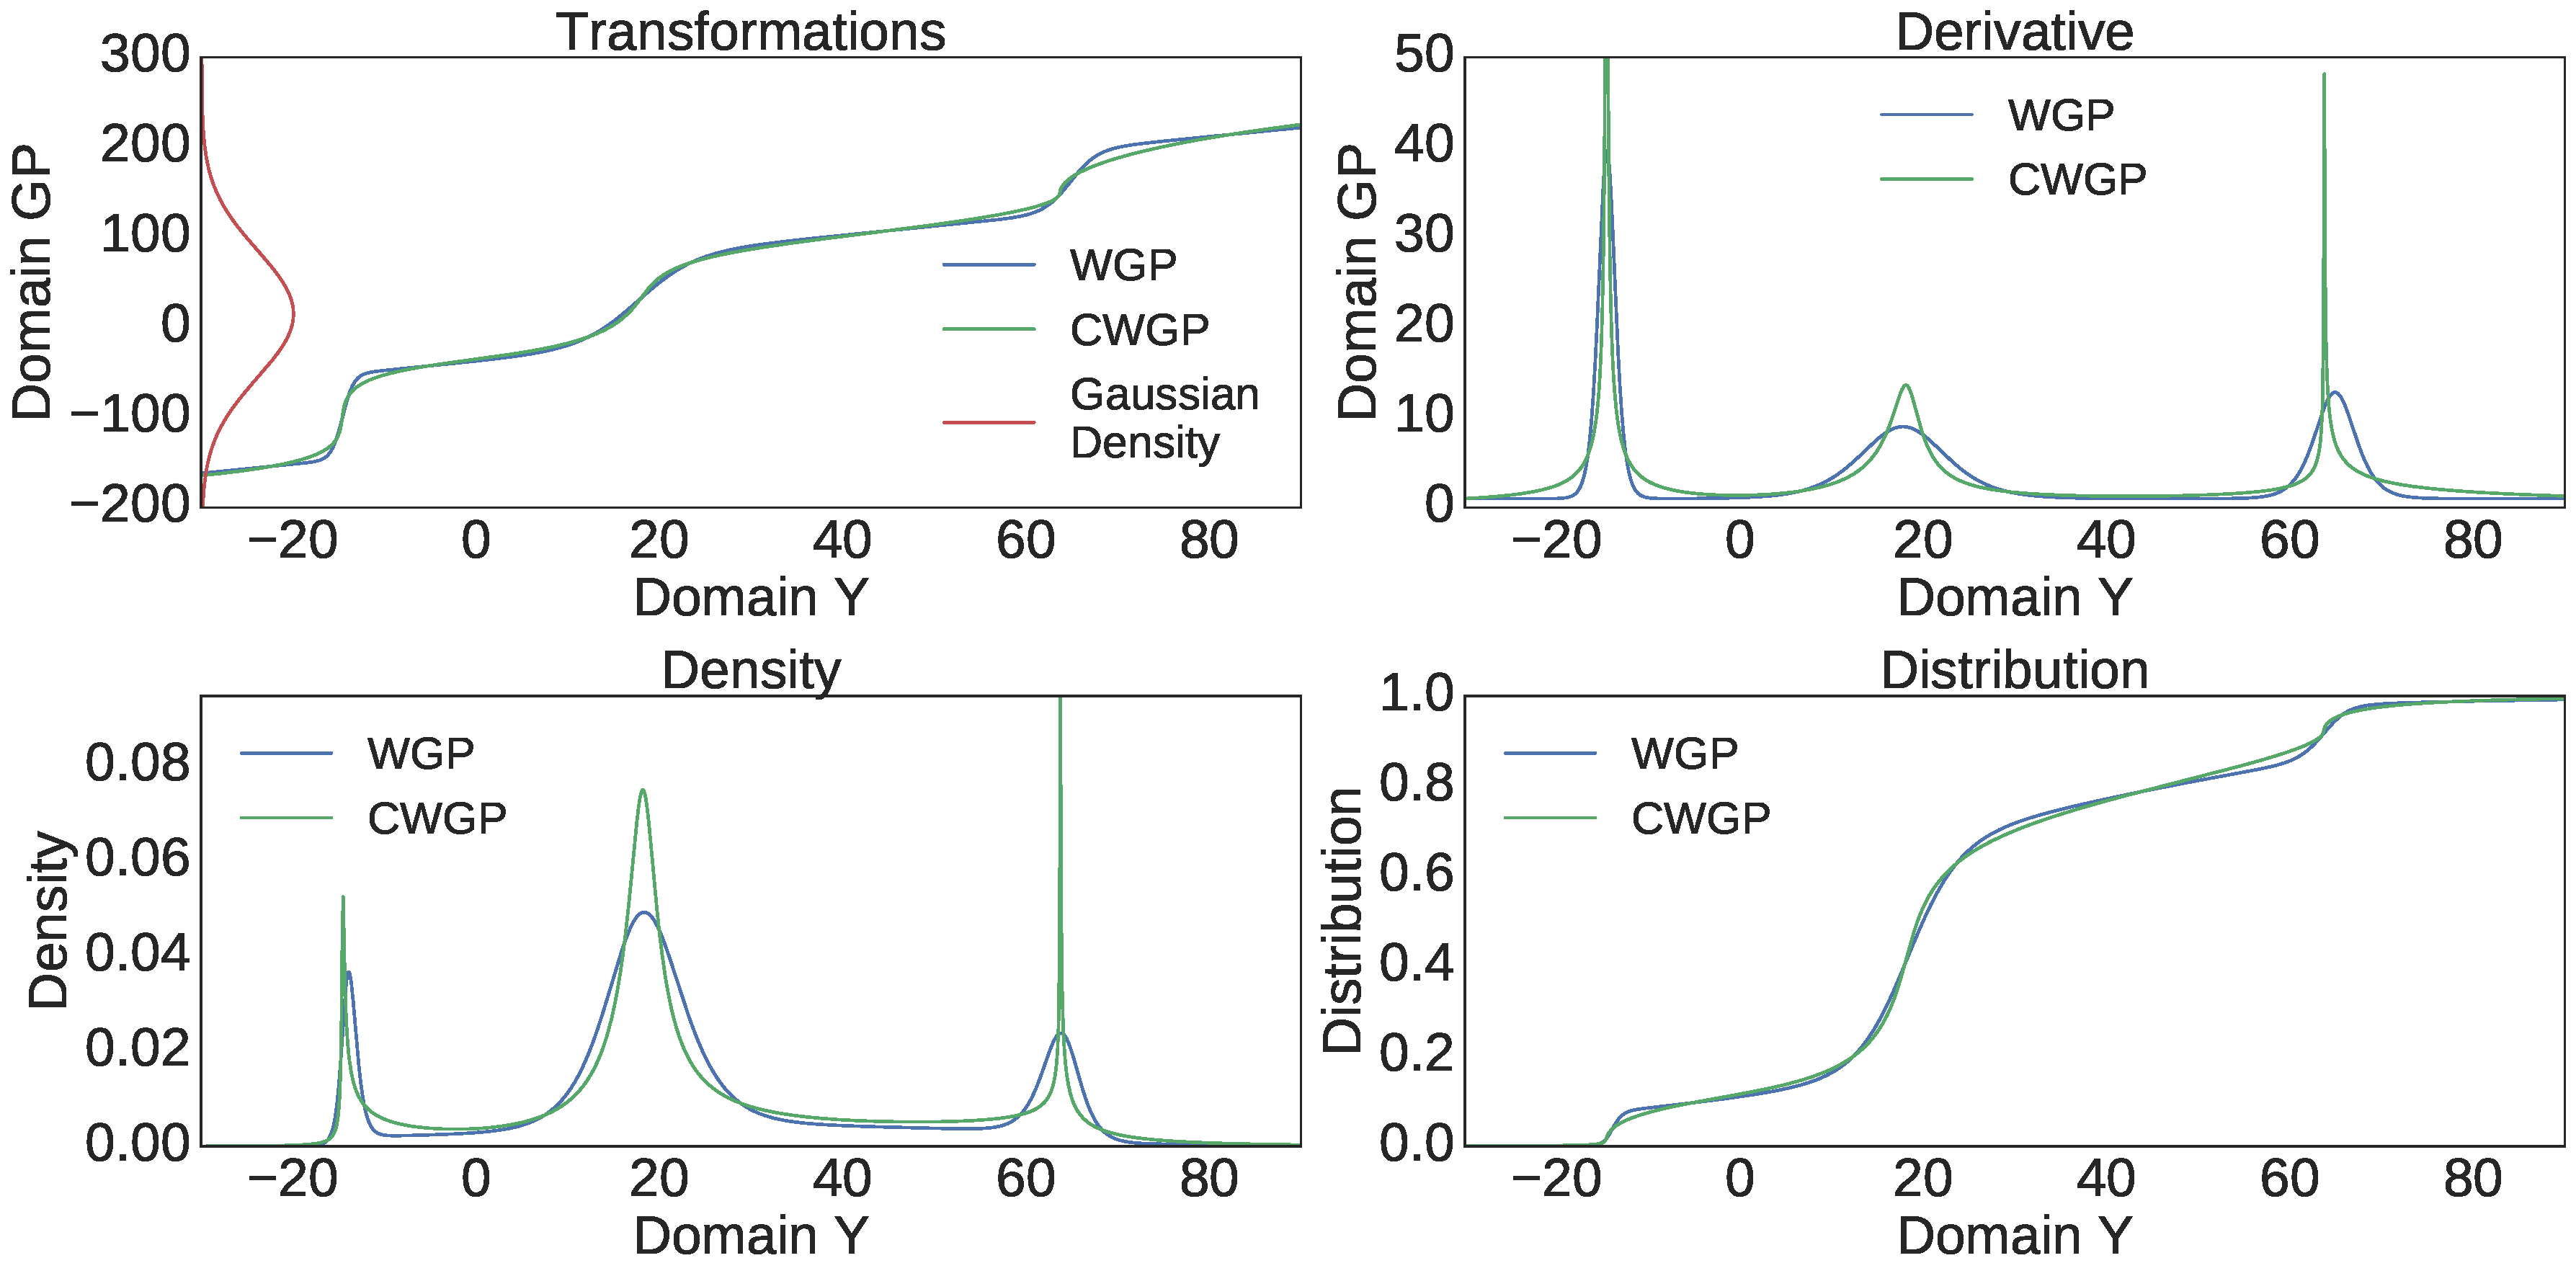
\includegraphics[width=0.8\textwidth]{cwgp_flexible}
	\caption{Aproximación de una deformación WGP (suma de tres tangentes hiperbólicas, en azul) usando el método por composición propuesto (tres capas SAL, en verde).}
	\label{fig:cwgp_flexible}
\end{figure}

Sobre la expresividad del enfoque por composición propuesto como una función del número de capas SAL consideradas, la figura \ref{fig:cwgp_blackbox1} muestra las distribuciones inducidas para un WGP con una deformación de cinco tangentes hiperbólicas (en azul) y aquellas de las aproximaciones compuestas usando de una a seis capas (en verde), ajustadas por mínimos cuadrados. Notemos cómo las distribuciones aprendidas por la transformación compuesta se vuelven indistinguibles de la verdad básica cuando el número de capas SAL crece.

\begin{figure}[h]
	\centering
	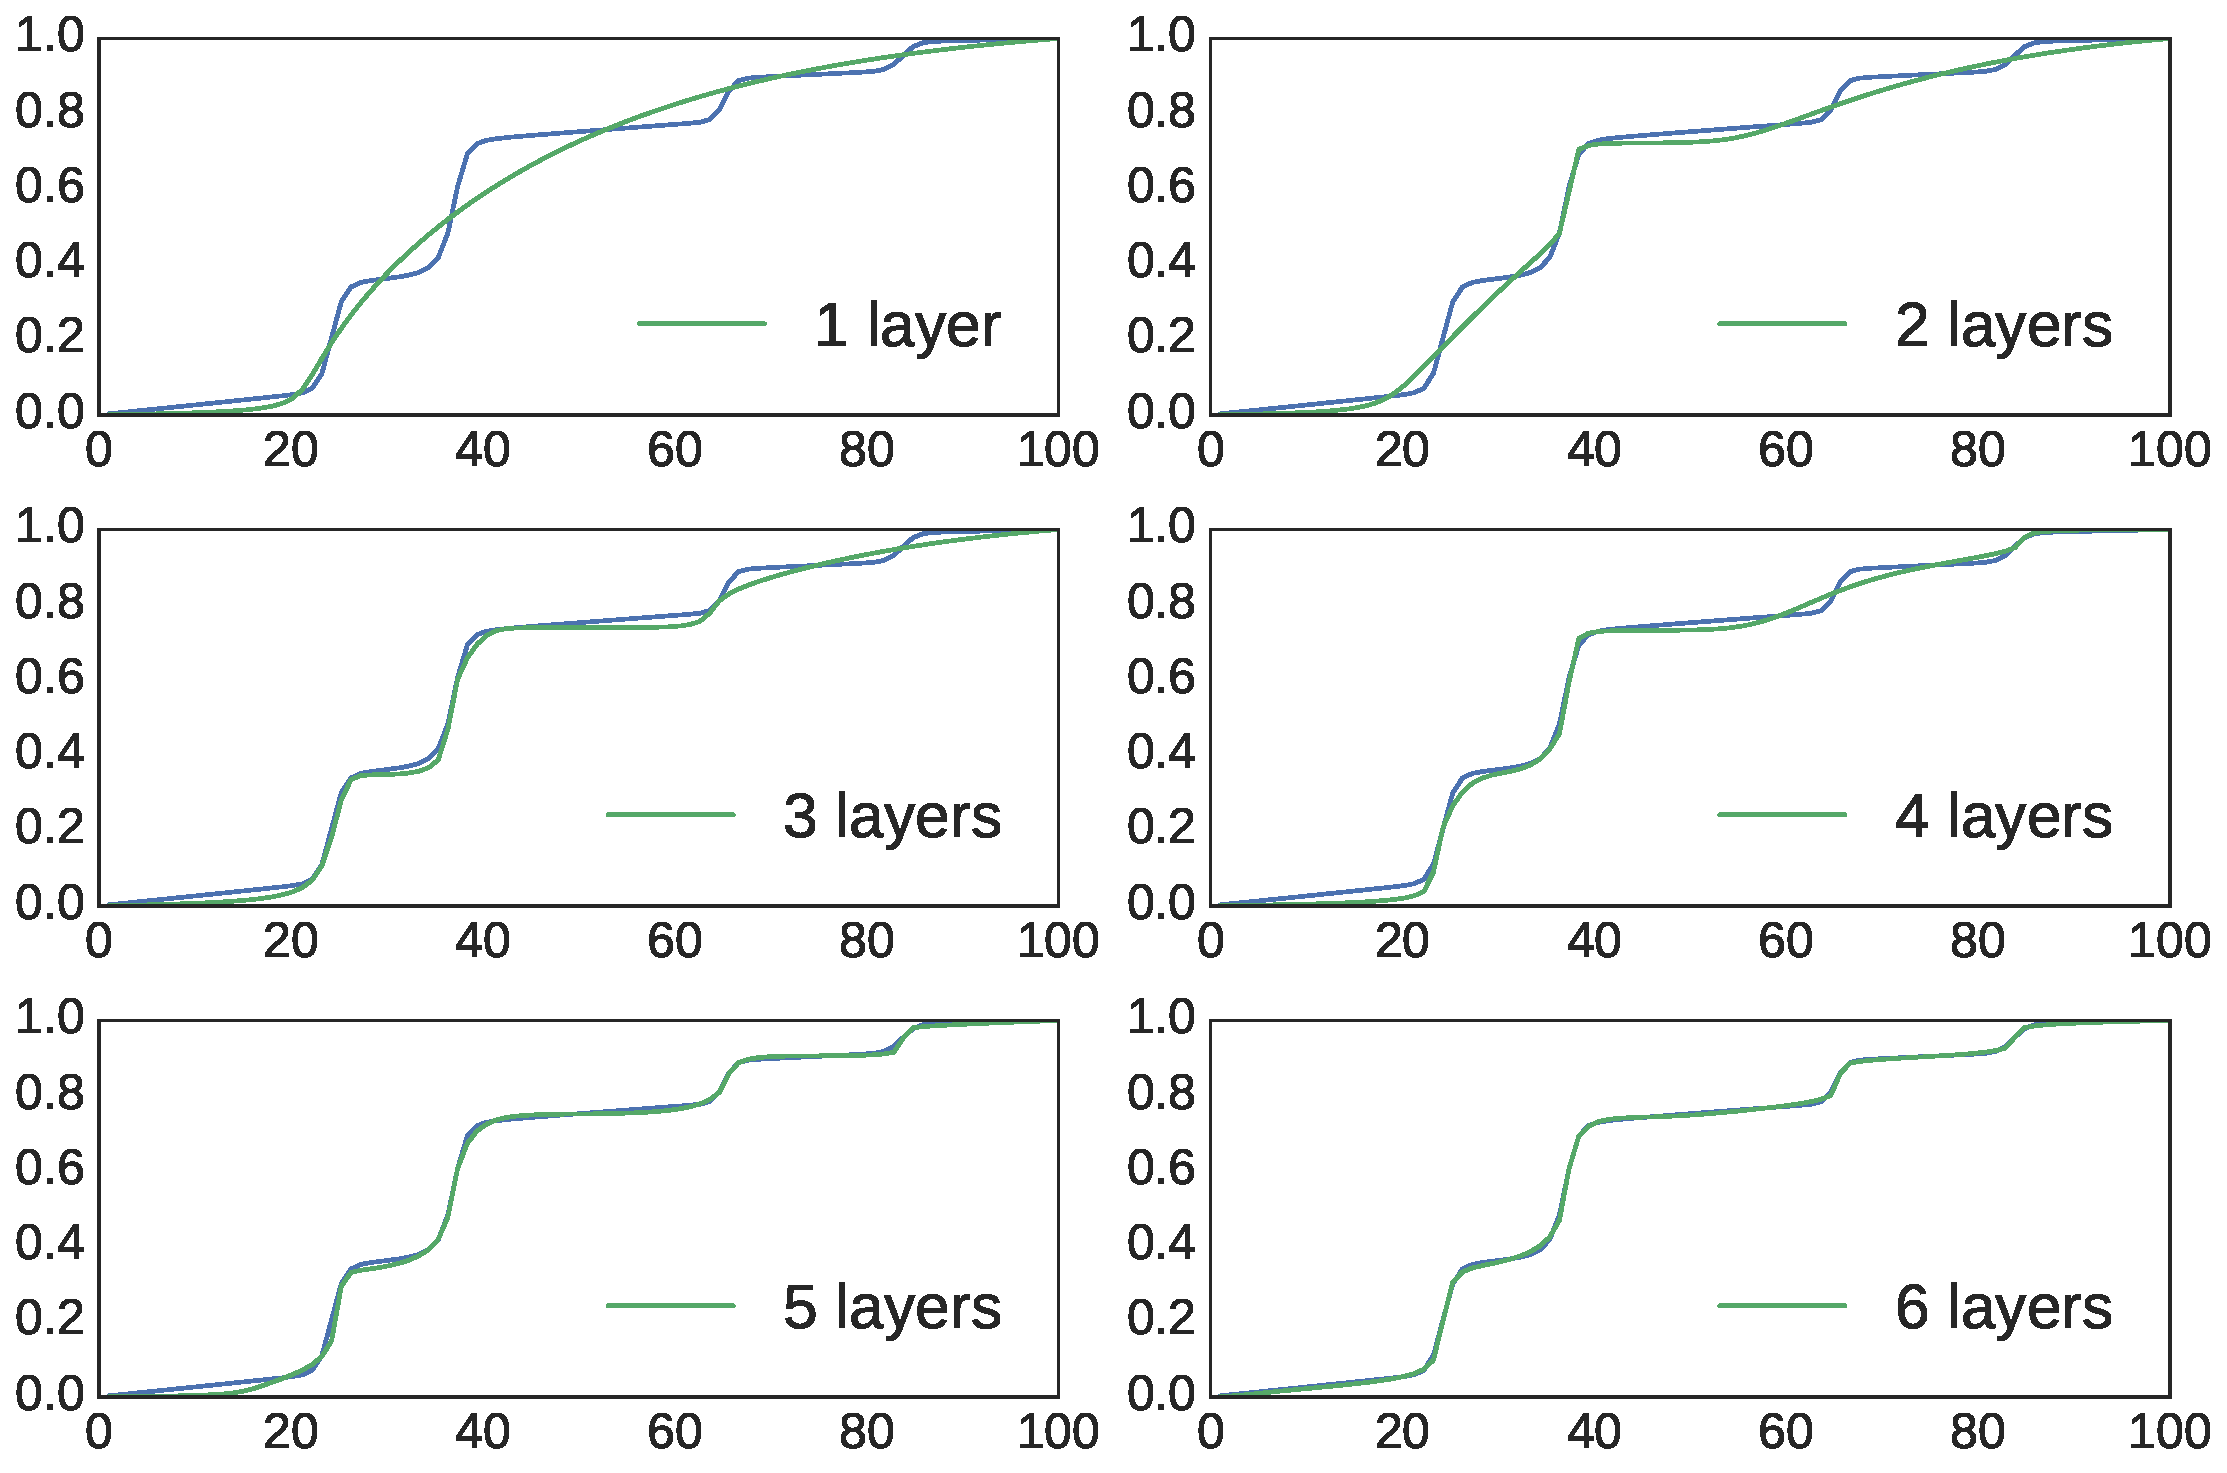
\includegraphics[width=0.7\textwidth]{cwgp_blackbox1}
	%\vspace{-1.5em}
	\caption{Aproximación CWGP de la distribución de un WGP con cinco tangentes hiperbólicas: la verdad básica (en azul) y las aproximaciones del CWGP (en verde), usando un número variable de capas SAL de la ecuación \eqref{eq:layer}.}
	\label{fig:cwgp_blackbox1}
	%\vspace{-1em}
\end{figure}

El cuadro \ref{tab:table_blackbox} reporta los errores de aproximación tanto para la transformación como para la distribución (deformada) resultante, usando las normas \(L_1\), \(L_2\) y \(L_\infty\) dadas por
%\begin{alignat*}{3}
%	e_1 &=||f_{\text{SoT}}-f_{\text{CT}}||_1 &&=\int_\reals|f_{\text{SoT}}(x)-f_{\text{CT}}(x)|dx\\
%	e_2 &=||f_{\text{SoT}}-f_{\text{CT}}||_2 &&=\sqrt{\int_\reals|f_{\text{SoT}}(x)-f_{\text{CT}}(x)|^2dx}\\
%	e_\infty &=||f_{\text{SoT}}-f_{\text{CT}}||_\infty &&=\sup_{x\in\reals}|f_{\text{SoT}}(x)-f_{\text{CT}}(x)|,
%\end{alignat*}
\begin{align*}
	e_1			&= \lVert f_{\mathrm{SdT}}-f_{\mathrm{TC}}\rVert_1 = \int_\reals \lvert f_{\mathrm{SdT}}(x) - f_{\mathrm{TC}}(x) \rvert \dd{x}\\
	e_2			&= \lVert f_{\mathrm{SdT}}-f_{\mathrm{TC}}\rVert_2 = \sqrt{\int_\reals \lvert f_{\mathrm{SdT}}(x) - f_{\mathrm{TC}}(x) \rvert^2 \dd{x}}\\
	e_\infty	&= \lVert f_{\mathrm{SdT}}-f_{\mathrm{TC}}\rVert_\infty = \sup_{x \in \reals} \lvert f_{\mathrm{SdT}}(x) - f_{\mathrm{TC}}(x) \rvert,
\end{align*}
donde \(f_{\mathrm{SdT}}\) denota a la transformación (o distribución) de la \emph{suma de tangentes hiperbólicas} del WGP, y \(f_{\mathrm{CT}}\) denota a aquellas de la \emph{transformación compuesta} propuesta. La figura \ref{fig:cwgp_blackbox2} muestra además las medidas de error antes descritas normalizadas con respecto al caso de una capa; notemos el desempeño monótono de la aproximación a medida de que el número de capas SAL aumenta.

\setlength{\tabcolsep}{4.4pt}
\begin{table}[h]
	\centering
	\begin{tabular}{crrrrrr}
		\toprule
		Capas	& Trans. \(L_1\)	& Trans. \(L_2\)	& Trans. \(L_\infty\)	& Dist. \(L_1\)	& Dist. \(L_2\)	& Dist. \(L_\infty\) \\
		\midrule
		1		& 1878.2			& 243.11			& 60.57					& 3.342			& 0.464			& 0.147 \\
		2		& 1147.7			& 151.86			& 33.77					& 2.232			& 0.292			& 0.107 \\
		3		&  845.14			& 124.80			& 37.19					& 1.628			& 0.192			& 0.047 \\
		4		&  582.53			&  83.71			& 27.34					& 1.464			& 0.184			& 0.041 \\
		5		&  319.64			&  41.33			& 15.28					& 0.793			& 0.115			& 0.057 \\
		6		&  147.78			&  19.95			&  6.48					& 0.316			& 0.042			& 0.015 \\
		7		&   91.64			&  15.71			&  8.32					& 0.174			& 0.025			& 0.011 \\
		\bottomrule
	\end{tabular}
	\caption{Aproximación «caja negra» de una deformación WGP con cinco tangentes hiperbólicas: medidas de error \(L_1\), \(L_2\) y \(L_\infty\) para las transformaciones y distribuciones inducidas, variando el número de capas.}
	\label{tab:table_blackbox} 
\end{table}

\begin{figure}[h]
	\centering
	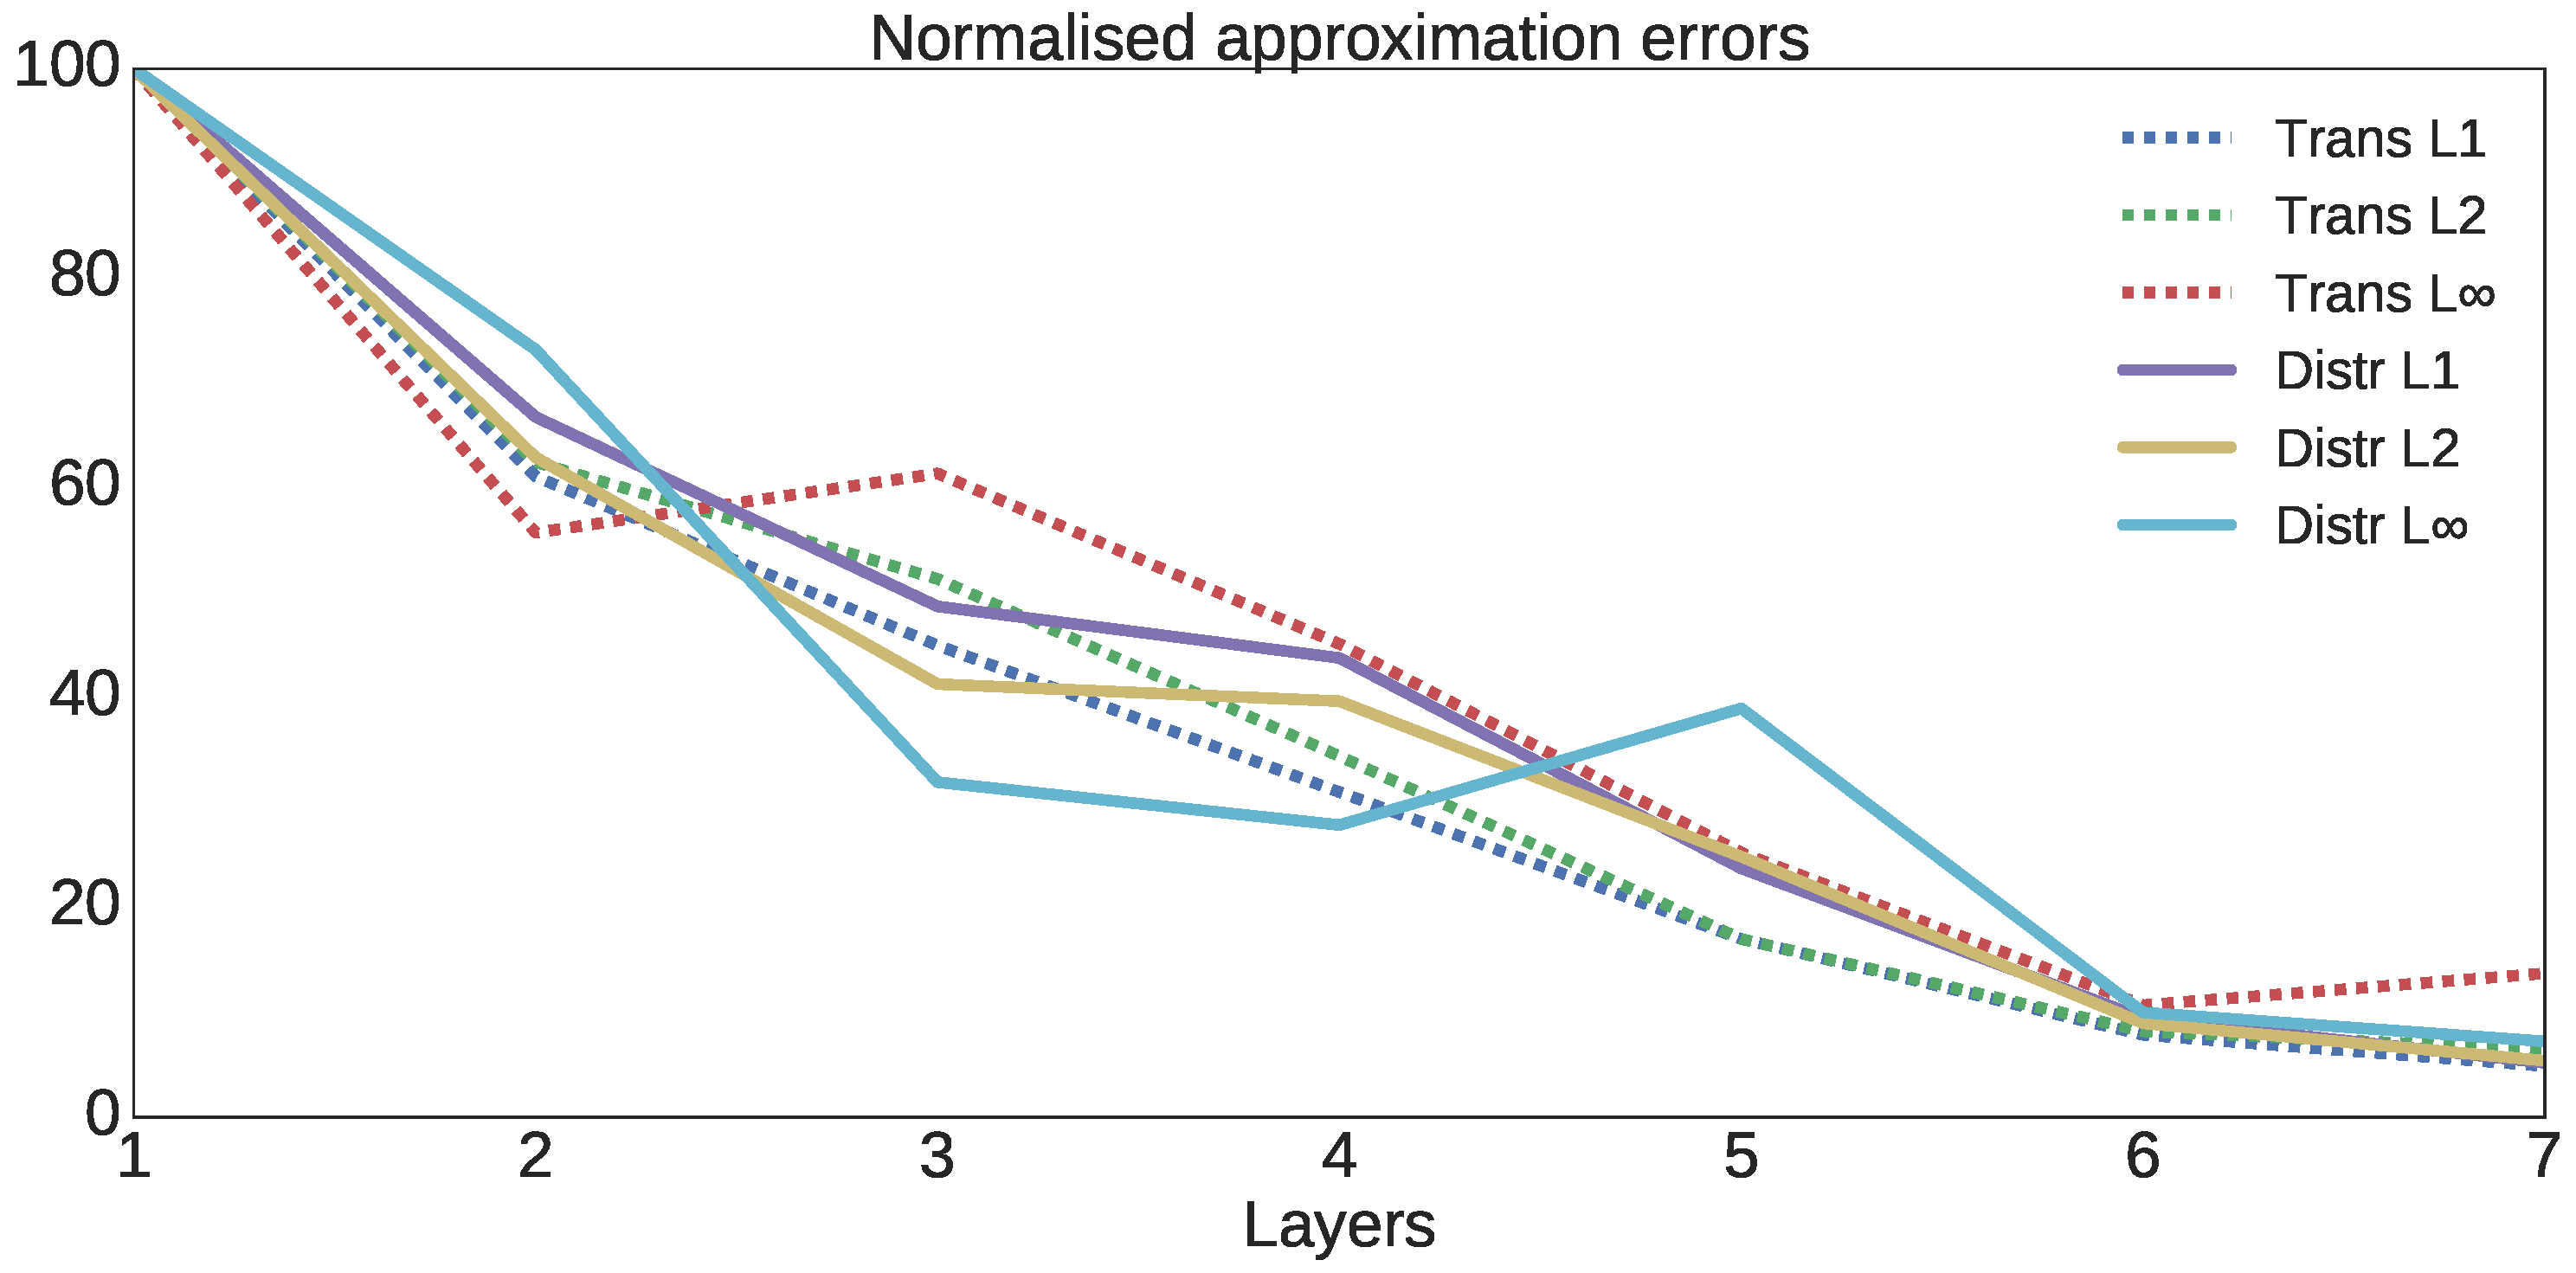
\includegraphics[width=0.7\textwidth]{cwgp_blackbox2}\\
	%\vspace{-1.5em}
	\caption{Representación de las medidas de error del cuadro \ref{tab:table_blackbox} normalizadas con respecto al error del caso de una capa.}
	\label{fig:cwgp_blackbox2}
	%\vspace{-1em}
\end{figure}


\comment{parrafo: falta la conclucion de capitulo, repasar lo mencionado, mencionar aplicaciones, limitantes, bondades y motivar la lectura en otros temas, mecionar temas similares o adyacentes}
	%!TEX root = main.tex

\chapter{Procesos Gaussianos Transportados}

\begin{chapquote}{Gonzalo Ríos, 2023}
	``Aquí falta una cita.''
\end{chapquote}

En el capítulo \ref{sec:tgp} deseamos explorar los límites teóricos de la expresividad de los CWGP, y aprovechar el principio basado en composición para unificar otros modelos no gaussianos bajo el mismo punto de vista. La contribución principal es un procedimiento nuevo propuesto para construir procesos estocásticos, en la sección \ref{sec:deftgp}, llamados \emph{procesos gaussianos transportados} (TGP por sus siglas en inglés, \emph{Transport Gaussian Processes}, al componer transformaciones o mapeos de transporte \cite{marzouk2016introduction}. Introducimos tres tipos de transportes diferentes que nos permiten aislar características específicas de los procesos estocásticos: las coordenadas marginales (en la sección \ref{sec:marginaltransport}), la covarianza y la correlación (en la sección \ref{sec:covariancetransport}) y la cópula intrínseca \cite{wilson2010copula} (e la sección \ref{sec:familytgp}), estableciendo así la fuerza de dependencia entre las coordenadas. En cada sección determinamos la forma de componer estos transportes para generar distribuciones que satisfacen las condiciones de consistencia de Kolmogorov \cite{tao2011introduction}, además de derivar sus fórmulasy métodos para predecir y aprender. En la sección \ref{sec:computationtgp} describimos algunos aspectos computacionales para la implementación de las familias de los procesos estocásticos que el enfoque TGP permite expresar, incluyendo GP, WGP, procesos de \(t\) de Student \cite{shah2014student}, abarcando procesos elípticos generales \cite{owen1983class} y arquimedianos \cite{mcneil2009multivariate}. El procesos de \(t\) de Student estrictamente más flexible debido a colas más pesadas, estabilidad frente a valores atípicos y estructuras de dependencia más sólidas, gracias a su cópula no gaussiana. Sin embargo, los PS son vistos de manera diferente a los modelos discutidos anteriormente y, hasta la fecha, no conocemos ningún trabajo que los relacione de alguna manera. Finalmente, en la sección \ref{sec:experimentstgp} validamos nuestro modelo propuesto con ejemplos de datos reales.


\section{Teorema de Consistencia de Kolmogorov}

\comment{este va aca o en el marco teorico??}
La principal dificultad para generalizar la idea de transformar un proceso estocástico de referencia es que la transformación debe evaluarse sobre los caminos del proceso, y excepto en casos específicos como las transformaciones de coordenadas, no se puede implementar como modelos prácticos. Mientras que el enfoque de la teoría de la medida para procesos estocásticos comienza con un espacio de probabilidad, en el aprendizaje automático el punto de partida es una colección de distribuciones de dimensión finita.


El bien conocido \emph{teorema de consistencia de Kolmogorov} \cite{tao2011introduction} garantiza que dada una adecuada colección \emph{consistente} de distribuciones \(\calF = \{\eta_{t_{1},...,t_{n}}| t_{1},...,t_{n} \in \mathcal{T}, n\in \naturals \}\) define un proceso estocástico \(f=\{x_{t}\}_{t\in \mathcal{T}}\), con leyes finito dimensiones \(\calF\). Por abuso de notación, su ley es denotada como \(\eta\). Denotando por \(F_{t_{1},...,t_{n}}(x_1,...,x_n)\) la función de distribución acumulada de \(\eta_{t_{1},...,t_{n}}\), las condiciones de \emph{consistencia}  sobre \(\calF\) son:
\begin{enumerate}
	\item Condición de permutación: \(F_{t_{1},...,t_{n}}\left( x_{1},...,x_{n}\right) =F_{t_{\tau \left( 1\right)},...,t_{\tau \left( n\right) }}\left( x_{\tau \left( 1\right) },...,x_{\tau\left( n\right) }\right)\) para todo \(t_1,...,t_{n} \in \calT\), para todo \(x_1,...,x_n \in \calX\) y cualquier \(n\)-permutación \(\tau\).
	\item Condición de marginalización: \(F_{t_{1},...,t_{n+m}}\left( x_{1},...,x_{n},+\infty,...,+\infty \right) =F_{t_{1},...,t_{n}}\left( x_{1},...,x_{n}\right)\) para todo \(t_1,...,t_{n+m} \in \calT\) y para todo \(x_1,...,x_n \in \calX\).
\end{enumerate}

La idea principal que desarrollamos en este capítulo es, para un proceso estocástico de referencia \(f\) dado y fijo, \emph{llevar hacia adelante}\footnote{Dada una medida \(\eta\) y un mapa medible \(\varphi\), la \emph{imagen directa} de \(\eta\) por \(\varphi\) es la medida definida como \(\varphi\#\eta = \eta(\varphi^{-1}(\cdot))\).} cada una de sus leyes de dimensión finita \(\eta_{\bft} \in \calF\) mediante algunos mapas medibles\footnote{Dado que el conjunto de todos los mapas medibles indexados \(T_{\bft}\) contiene información sobre todas las coordenadas, por abuso de notación se denota como \(T\).} \(T_{\bft} \in T\), para generar un nuevo conjunto de distribuciones de dimensión finita \(\mathcal{\hat F}\) y, por lo tanto, un proceso estocástico. La principal dificultad de este enfoque es que, en general, \(\mathcal{\hat F}\) puede ser inconsistente, en el sentido de que puede violar algunas condiciones de consistencia; sin embargo, es posible elegir los mapas que inducen un conjunto consistente de leyes de dimensión finita y, por lo tanto, un proceso estocástico.



La idea principal es construir procesos estocásticos, compuestos de diferentes \emph{capas}, siguiendo las mismas directrices que las arquitecturas profundas, pero donde cada capa tiene una interpretación que define una característica del proceso. En este capítulo definimos cuatro tipos de transportes finito-dimensionales, que pueden verse como capas elementales para nuestro modelo de regresión propuesto. Nuestro enfoque comienza desde un proceso de ruido de proceso gaussiano de referencia, ya que es un proceso bien conocido con densidad explícita y métodos de muestreo eficientes, para generar procesos estocásticos más expresivos. El enfoque propuesto puede modelar cópulas y marginales no gaussianas, más allá de los conocidos WGP \cite{snelson2004warped, rios2018learning, riostobar2019cwgp} y SP \cite{shah2014student}, pero incluyéndolos a todos desde un punto de vista unificador. La primera capa determina la \emph{cópula} del proceso inducido, que puede ser elíptica a través de transportes elípticos. En el caso elíptico, es posible componerlo con un transporte de covarianza para determinar la correlación en el proceso estocástico inducido. Finalmente, en cualquier caso, podemos componer cualquier número de transportes marginales para definir una distribución marginal expresiva sobre el proceso estocástico inducido, como se muestra en el trabajo anterior \cite{riostobar2019cwgp}. Como vimos en las secciones anteriores, estas composiciones son consistentes y lo suficientemente expresivas como para incluir GPs, WGPs, SPs, procesos elípticos, y aquellos que podríamos llamar \emph{procesos elípticos deformados}.


Nuestra principal contribución es entender la consistencia en las composiciones, derivar expresiones analíticas generales para sus distribuciones posteriores y funciones de verosimilitud, y desarrollar métodos prácticos para la inferencia y entrenamiento de nuestro modelo, dada la información. El resto de este capítulo se organiza de la siguiente manera. En la sección \ref{sec:introductiontgp}, presentamos la notación y el conocimiento matemático necesario para desarrollar nuestro trabajo. Nuestra principal definición está en la sección \ref{sec:deftgp}, donde proponemos el proceso transportado (TP) y el enfoque de inferencia. En la sección \ref{sec:marginaltransport}, estudiamos el transporte marginal que aísla todas las propiedades sobre las marginales univariadas del TP. De manera similar, en la sección \ref{sec:covariancetransport}, desarrollamos el transporte de covarianza, que determina la correlación sobre el TP. Finalmente, la principal contribución está en la sección \ref{sec:familytgp}, donde presentamos los transportes radiales, que nos permiten definir la estructura de dependencia (también conocida como cópula) sobre el TP. En la sección \ref{sec:computationtgp}, profundizamos en detalles sobre la implementación computacional y algorítmica, y en la sección \ref{sec:experimentstgp} validamos nuestro enfoque con datos del mundo real.


\section{Cópulas}

\comment{este va aca o en el marco teorico??}
Como vimos en el capítulo \ref{sec:cwgp}, un WGP define modelos no gaussianos con propiedades matemáticas atractivas y similares a los GP, como tener expresiones con fórmula cerrada para hacer inferencia y aprender. Sin embargo, heredan una desventaja gaussiana que no es deseada: la estructura de dependencia, llamada cópula, sigue siendo puramente gaussiana. Para entender las implicaciones de este problema, necesitamos formalizar el concepto de dependencia. A continuación fijaremos un poco de notación y convenciones.

Dada una distribución multivariada \(\eta\), denotamos por \(F_\eta\) a su función de distribución acumulada. Siempre que no haya ambigüedad, denotaremos a la función de distribución acumulada de su \(i\)-ésima distribución marginal \(\eta_{i}\) por \(F_i(x) \coloneqq F_{\eta_i}(x)\), así como a su función de cuantil continua-por-la-derecha \(Q_i(u) \coloneqq F_i^{-1}(u) = \inf \{x \mid F_i(x) \geq u\}\). Si una función de distribución acumulada multivariada \(C\) tiene marginales univariadas uniformes en \([0, 1]\), es decir, \(C_i(u) = \max\{0, \min\{u, 1\}\}\) para \(i = 1, \dotsc, n\), entonces decimos que \(C\) es una \emph{cópula}. El siguiente resultado, llamado el Teorema de Sklar \cite{sklar1959fonctions}, muestra que cualquier distribución tiene una cópula asociada.

\begin{theorem}[Sklar]
	Dada una distribución multivariada \(\eta\), existe una cópula \(C\) tal que
	\[F_{\eta}(x_{1}, \dotsc, x_{n}) = C(F_{1}(x_{1}), \dotsc, F_{n}(x_{n})).\]
	Si las \(F_i\) son continuas, para \(i = 1, \dotsc, n\), entones la cópula es única y está dada por
	\[C_{\eta}(u_{1}, \dotsc, u_{n}) = F_{\eta}(F^{-1}_{1}(u_{1}), \dotsc, F^{-1}_{n}(u_{n})).\]
\end{theorem}

Si \(\eta\) es una distribución gaussiana, su única cópula tiene una densidad que está determinada exclusivamente por su matriz de correlación \(R\), y está dada por
\[C_{\eta}(\bfu) = \frac{\exp \left(-\frac{1}{2} \bfx^{\top} [R^{-1} - I] \bfx\right)}{\sqrt{\det(R)}},\]
donde \(x_i = F_{s}^{-1}(u_i)\) y \(F_{s}\) es la función de distribución acumulada de la normal estándar. Notemos que si sus coordenadas no están correlacionadas, entonces \(C_\eta\) coincide con la cópula de independencia. Para modelos gaussianos, la correlación y la dependencia son equivalentes. Sin embargo, más allá de la esfera de la gaussianidad, este no es el caso. Algunas variables pueden no estar correlacionadas y mostrar dependencia en eventos inusuales, como muestran los casos de crisis financieras o desastres naturales. Desafortunadamente, como se describe a continuación, la cópula gaussiana no es la adecuada para estos tipos de dependencias estructurales.

La dependencia entre dos variables aleatorias es más compleja que solo considerar la correlación, destacando un concepto de la teoría de valores extremos: dependencia de colas \cite{coles2001introduction}. Definimos los coeficientes inferior y superior de la dependencia de colas \cite{schmidt2005tail} entre dos variables aleatorias \(X_{1}\) y \(X_{2}\) como
\begin{align*}
	\lambda_{l}	&= \lim_{q \to 0} \prob\left(X_{2} \leq F_{2}^{-1}(q) \mid X_{1} \leq F_{1}^{-1}(q)\right)\\
	\lambda_{u}	&= \lim_{q \to 1} \prob\left(X_{2} > F_{2}^{-1}(q) \mid X_{1} > F_{1}^{-1}(q)\right),
\end{align*}
donde \(F_i\) es la función de distribución acumulada de \(X_i\) para \(i = 1, 2\). Estos coeficientes proveen de métricas asintóticas de la dependencia en las colas (valores extremos), que están aislados de sus distribuciones marginales. Para variables aleatorias continuas e independientes tenemos que \(\lambda_{l} = \lambda_{u} = 0\), mientras que para variables con una correlación de \(\rho = 1\) tenemos que \(\lambda_{l} = \lambda_{u} = 1\). Para distribuciones gaussianas se tiene un resultado interesante: para una correlación \(\rho < 1\) tenemos que \(\lambda_{l} = \lambda_{u} = 0\).

El resultado anterior implica que las variables gaussianas son \emph{asintóticamente independientes}, lo que quiere decir que la suposición de gaussianidad no permite modelar la dependencia de valores extremos. Esta incapacidad, heredada por cualquier transformación diagonal, puede resultar en cálculos engañosos de las probabilidades sobre casos extremos. Este problema fue observado mayoritariamente en la crisis \emph{subprime} de 2008, en donde se señaló que la estructura de dependencia gaussiana fue una de las principales causas, evidenciando así que «\emph{the devil is in the tails}»\footnote{N. de los A.: juego de palabras intraducible, en donde se mezclan la jerga en inglés \emph{the devil is in the details} («el diablo está en los detalles») y la palabra \emph{tails} («colas»).} \cite{donnelly2010devil}. Construir procesos estocásticos que den cuenta de la dependencia de las colas es un desafío, pues en general las distribuciones que satisfacen las condiciones de consistencia son escasas.


\section{Proceso Transportado}
\label{sec:deftgp}


La siguiente definición es una de nuestras principales contribuciones, ya que nos permite construir procesos no Gaussianos como modelos de regresión no paramétricos.

\begin{definition}
	Sea \(T=\{T_\bft:\calX^n \to \calY^n \subseteq \reals^n | \bft \in \calT^n, n \in \mathbb{N}\}\) una colección de mapas medibles y \(f=\left\{x_{t}\right\}_{t\in \calT}\) un proceso estocástico con ley \(\eta\). Decimos que \(T\) es un transporte de \(f\) si las distribuciones finito-dimensionales push-forward \(\mathcal{\hat F}=\{\pi_{\bft}:=T_{\bft}\#\eta_{\bft}| \bft \in \calT^n, n \in \naturals\}\) son consistentes y definen un proceso estocástico \(g=\left\{ y_{t}\right\}_{t\in \calT}\) con ley \(\pi\). En este caso, decimos que los mapas \(T\bft\) son \(f\)-consistentes, y que \(T(f) := g\) es un proceso transportado (TP) con ley denotada como \(T\#\eta := \pi\).
\end{definition}

La idea principal de la definición anterior es partir de un proceso estocástico simple, uno que sea fácil de simular, y luego generar otro proceso estocástico que sea más complejo y expresivo. Dado que nuestro propósito es modelar los datos a través de sus leyes de dimensionalidad finita, nuestra definición implica una correspondencia entre las leyes del proceso de referencia y las del proceso objetivo; por esta razón, es importante que los mapeos mantengan el tamaño de las distribuciones y los índices respectivos.

Es evidente que hay muchas colecciones de mapas medibles que son inconsistentes, incluso en algunos casos simples. Por ejemplo, consideremos los mapas de intercambio dados por \(T_1(x_1) = x_1\) y \(T_{12}(x_1,x_2) = (x_2,x_1)\). Si \(f\) es un proceso gaussiano heterocedástico, entonces tenemos \(F_1(x_1) = \calN_1(x_1|0,\sigma_1^2)\) y \(F_{12}(x_1, x_2)=\calN_2\left((x_1, x_2)|0,\begin{bmatrix} \sigma_1^2 & \sigma_{12} \\ \sigma_{12} & \sigma_2^2 \end{bmatrix}\right)\). Las distribuciones push-forward se dan por \(G_1(y_1)=\calN_1(x_1|0,\sigma_1^2)\) y \(G_{12}(y_1,y_2)=\calN_2\left((y_1, y_2)\vert 0,\Sigma\right)\) con \(\Sigma = \begin{bmatrix} \sigma_2^2 & \sigma_{12} \\ \sigma_{12} & \sigma_1^2 \end{bmatrix}\), y dado que \(\lim\limits_{y_2 \to \infty} G_{12}(y_1,y_2) = \calN_1(x_1 \vert 0,\sigma_2^2) \neq \calN_1(x_1|0,\sigma_1^2) = G_1(y_1)\), tenemos que \(T\) es inconsistente para \(f\). Note que si \(f\) es un proceso estocástico trivial \emph{i.i.d.}, entonces \(T\) es \(f\)-consistente.

Para poder utilizar procesos de transporte como modelos de regresión, debemos ser capaces de definir un transporte finitamente parametrizado \(T^\theta\) con \(\theta \in \Theta \subset \reals^d\), donde los mapas finitamente dimensionales \((T^\theta)_\bft\) son consistentes e invertibles. Por ejemplo, dado \(\theta \in \Theta = \calX\), el transporte de \emph{desplazamiento} es \(T^\theta =\{T_{\bft}(\bfx) = \bfx + \theta | \bft \in \calT^n, n \in \mathbb{N}\}\), o simplemente \((T^\theta)_{\bft}(\bfx) = \bfx + \theta\). Para mayor simplicidad, si no hay ambigüedad, denotaremos \((T^\theta)_\bft\) como \(T_\bft\). En las próximas secciones, mostraremos ejemplos más sofisticados de transportes finitamente parametrizados \(T^\theta\), por lo que en lo que sigue nos concentraremos en explicar el enfoque general de utilizar TP como modelos de regresión.

\subsection{Entrenamiento de un proceso transportado}

Como en el enfoque de los procesos gaussianos, dadas las observaciones, la tarea de aprendizaje corresponde a encontrar el \emph{mejor} transporte \(T^\theta\), determinado por los parámetros \(\theta\) que minimizan el logaritmo negativo de su verosimilitud marginal (NLL, por sus siglas en inglés), que se muestra a continuación.

\begin{proposition}
	Sea \(g = T^\theta(f)\) un proceso transportado con ley \(\pi = T^\theta\#\eta\), donde \(\eta\) tiene distribuciones finito dimensionales con densidad denotada \(\eta_{\bft}\). Dadas las observaciones \((\bft,\bfy)\), si el mapeo \(T_\bft\) es invertible en \(\bfy\) (por simplicidad denotamos \(T_\bft^{-1}\) como \(S_\bft\)) y diferenciables en \(\bfx=S_\bft(\bfy)\), su NLL está dada por
	\begin{align}
	\label{eq:TGP_NLL}
	-\log \pi_{\bft}(\bfy|\theta) &= -\log \eta_{\bft}(S_{\bft}(\bfy)) - \log |\nabla S_{\bft}(\bfy)|\nonumber\\
	&= -\log \eta_{\bft}(S_{\bft}(\bfy)) + \log |\nabla T_{\bft}(S_{\bft}(\bfy))|.
	\end{align}
\end{proposition}
La primera igualdad es debido a la fórmula del cambio de variable \cite{hogg1995introduction}. Para ls segunda identidad, gracias al teorema de la función inversa \cite{rudin1964principles} tenemos que \(\nabla S_{\bft}(\bfy) = \nabla T_{\bft}(\bfx)^{-1}\), y por la propiedad del determinante de la inversa \cite{petersen2008matrix} obtenemos que \(|\nabla T_{\bft}(\bfx)^{-1}| = |\nabla T_{\bft}(\bfx)|^{-1}\). Para calcular eq.~\eqref{eq:TGP_NLL} necesitamos ser capaces de computar la log densidad de \(\eta_{\bft}\), la inversa \(S_{\bft}\), y el gradiente \(\nabla T_{\bft}\) (o \(\nabla S_{\bft}\)).

Es importante destacar que el proceso de referencia está fijo y el objeto entrenable corresponde al transporte. En otras palabras, siguiendo el principio conocido como \emph{truco de reparametrización} \cite{kingma2013auto}, el modelo se define de tal manera que las fuentes aleatorias no tienen parámetros, de modo que los algoritmos de optimización se puedan aplicar sobre funciones paramétricas deterministas. Al igual que en el enfoque de GP, el NLL para el proceso transportado (ec.~\eqref{eq:TGP_NLL}) sigue una interpretación elegante de cómo evitar el sobreajuste.

\begin{itemize}
	\item El primer término \(-\log \eta_{\bft}(S_{\bft}(\bfy))\) es la \emph{bondad de ajuste}, puntaje entre el modelo y los datos, privilegiando aquellos parámetros \(\theta\) que hacen \(S_{\bft}(\bfy)\) ser cercano a la moda de \(\eta_{\bft}\). Por ejemplo, si \(\eta_{\bft}\) es una normal estándar, este término (omitiendo la constante) es \(\frac{1}{2}\lVert S_{\bft}(\bfy) \rVert_{2}^2\), y con suficientes observaciones resulta en sobreajuste: \(S_{\bft}\) es la función nula.
	\item Por otro lado, el segundo término \(-\log |\nabla(S_{\bft}(\bfy)|\) es la \emph{penalización de la complejidad del modelo}, y prioriza aquellos parámetros \(\theta\) que hacen que \(|\nabla S_{\bft}(\bfy)|\) sea grande, es decir \(S_{\bft}\) tiene gran desviación en torno a \(\bfy\), evitando de este modo la función nula y, a su vez, el sobreajuste. Note que un mapeo válido satisface \(|\nabla S_{\bft}(\bfy)|>0\).
\end{itemize}  

\subsection{Inferencia con el proceso transportado}

Una vez que el transporte \(T^\theta\) está entrenado, a través de la minimización del NLL, la inferencia se realiza mediante el cálculo de la distribución posterior de \((\bfto, \bfyo)\) dado las observaciones \((\bft, \bfy)\) bajo la ley \(\pi\): para cualquier entrada \(\bfto\) calculamos las distribuciones posteriores \(\pi_{\bfto|\bft}(\cdot|\bfy)\). Como nuestro objetivo es generar procesos estocásticos más expresivos que los GP, la media y la varianza no son suficientes para calcular (por ejemplo, necesitamos expectativas asociadas con valores extremos). Por esta razón, nuestro enfoque se basa en generar de manera eficiente muestras independientes de \(\pi_{\bfto|\bft}\), para luego realizar cálculos mediante métodos de Monte Carlo \cite{rubinstein2016simulation}.

Dado que asumimos que podemos obtener fácilmente muestras de \(\eta_{\bfto}\) (y \(\eta_{\bfto|\bft}\) si es necesario), mostraremos cómo usar estas muestras y el transporte \(T^\theta\) para generar muestras eficientemente de \(\pi_{\bfto|\bft}\). El principio detrás de esta idea es que si \(\pi_{\bfto|\bft} = \varphi\#\eta_{\bfto}\) y \(\bfx \sim \eta_{\bfto}\), entonces \(\varphi(\bfx) \sim \pi_{\bfto|\bft}\). En casos en los que este principio no se pueda aplicar, podemos obtener muestras utilizando métodos basados en MCMC, que deben poder evaluar la densidad de la distribución posterior.


\section{Transporte Marginal}
\label{sec:marginaltransport}

En esta sección, presentamos una familia de transportes llamados \emph{transportes marginales}, dado que pueden cambiar las distribuciones marginales de un proceso estocástico, extendiendo de esta manera la función de media de las GPs, así como la función de deformación de las WGPs, incluyendo el modelo CWGP presentado anteriormente en el Capítulo \ref{sec:cwgp}. Demostramos su consistencia, entregamos las fórmulas para su entrenamiento y damos un método general para muestrear.

\begin{definition}
	\(T=\{T_\bft | \bft \in \calT^n, n \in \mathbb{N}\}\) es un transporte marginal si existe una función medible \(h: \calT \times \calX \rightarrow \calX\), tal que \([T_\bft(\bfx)]_i = h(t_i, x_i)\) para \(\bft \in \calT^n, \bfx \in \calX^n, n \in \mathbb{N}\). Adicionalmente, si \(h(t,\cdot):\calX \rightarrow \calX\) es creciente (por lo tanto diferenciable en casi todos los puntos) para todo \(t \in \calT\), entonces decimos que \(T\) es un transporte marginal creciente.
\end{definition}

Un transporte \emph{marginal} es definido de forma \emph{por coordenadas} por la función \(h\). Por ejemplo, dada una función de \emph{localización} \(m: \calI \rightarrow \calX\), entonces \(h(t,x) = m(t)+x\) induce un transporte marginal \(T^h\) tal que si \(\eta = \GP(0,k)\) entonces \(T^h\#\eta = \GP(m, k)\). Como \(T^h\) determina la media en el proceso estocástico inducido, elecciones usuales para \(m\) son funciones elementales tales como polinomios, exponenciales, funciones trigonométricas y combinaciones aditivas y multiplicativas.

Sin embargo, esta familia de transportes es más expresiva que la simple determinación de la media, pudiendo definir momentos superiores como la varianza, la asimetría y la curtosis. Esta expresividad puede lograrse, junto a la función de \emph{localización} \(m\), considerando una \emph{deformación} \(\varphi: \calY \rightarrow \calX\) para definir el transporte \(T^h\) inducido por la función compuesta \(h(t,x) = \varphi^{-1}\left(m(t)+x\right)\), tal que si \(\eta = \GP(0,k)\) entonces tenemos que \(T^{h}\#\eta = \WGP(\varphi, m, k)\). La funciones de \emph{deformación} más usuales son las funciones afines, logaritmo, Box-Cox \cite{rios2018learning}, and sinh-arcsinh \cite{Sinharcsinh}, las cuales se pueden componer para generar deformaciones más expresivas. Este modelo basado en capas, denominado WGP composicional, ha sido estudiado exhaustivamente en trabajos previos \cite{rios2018learning, riostobar2019cwgp}. Sin embargo, la expresividad del transporte marginal es más general ya que la función de deformación puede cambiar a lo largo de las coordenadas

\subsection{Consistencia del transporte marginal}

Los transportes marginales están bien definidos con una referencia de GP, en el sentido de que siempre define un conjunto de distribuciones finitamente dimensionales consistentes, y por lo tanto induce un proceso estocástico. La siguiente proposición muestra que esta familia de transportes es compatible con cualquier proceso estocástico, una propiedad que nos referimos como \emph{universalmente consistente}.

\begin{proposition}
	Dado cualquier proceso estocástico \(f=\left\{ x_{t}\right\}_{t\in \calT}\) y cualquier transporte marginal creciente \(T\), entonces \(T\) es un \(f\)-transporte.
	\begin{proof}
		Dada \(\eta_{\bft} \in \calF\) una distribución finito dimensional, la función de distribución acumulada transportada está dada por \(F_{\pi_{\bft}}(\bfy) = F_{\eta_{\bft}}((h^{-1}(t_i,y_i))_{i=1}^n)\), donde \(h^{-1}(t,\cdot)\) denota la inversa en la coordenada \(\calX\) de \(h\), la cuál también es incremental. 
		
		La condición de marginación se cumple ya que \(F_{\eta_{\bft,t_{n+1}}}(\bfx,\infty) = F_{\eta_{\bft}}(\bfx)\), entonces tenemos
		\begin{align*}
			F_{\pi_{\bft,t_{n+1}}}(\bfy,\infty) &= F_{\eta_{\bft,t_{n+1}}}((h^{-1}(t_i,y_i))_{i=1}^n, h^{-1}(t_{n+1},\infty)),\\
			&=F_{\eta_{\bft,t_{n+1}}}((h^{-1}(t_i,y_i))_{i=1}^n, \infty)
			=F_{\eta_{\bft}}((h^{-1}(t_i,y_i))_{i=1}^n)=F_{\pi_{\bft}}(\bfy).
		\end{align*}
		
		Dada una \(n\)-permutación \(\tau\), denotamos \(\tau(\bft) = t_{\tau(1)},...,t_{\tau(n)}\) y \(\tau(\bfy) = y_{\tau(1)},...,y_{\tau(n)}\). Dado \(F_{\eta_{\tau(\bft)}}(\tau(\bfx)) = F_{\eta_{\bft}}(\bfx)\) entonces  \(F_{\pi_{\tau(\bft)}}(\tau(\bfy)) =  F_{\eta_{\tau(\bft)}}((h^{-1}(t_{\tau(i)},y_{\tau(i)}))_{i=1}^n)=F_{\eta_{\bft}}((h^{-1}(t_i,y_i))_{i=1}^n)=F_{\pi_{\bft}}(\bfy)\), satisfaciendo las condiciones de consistencia de Kolmogorov. 
	\end{proof}
\end{proposition}

\begin{remark}
	En general supondremos que los transportes marginales son crecientes, debido a que para cualquier proceso estocástico fijo \(f\) y cualquier transporte marginal \(T\), existe un transporte marginal creciente \(T^h\) tal que \(T\#f\) y \(T^h\#f\) tienen la misma distribución (es decir todas sus distribuciones de dimensión finita coinciden \cite{shalizi2010almost}). La función creciente \(h\) se define a través de los mapas de transporte monótonos únicos de \(\eta_t\) a \(\pi_t\) dado por \(h(t,x) = F_{\pi_t}^{-1}(F_{\eta_t}(x))\) para cada \(t \in \calT\) \cite{cuestaalbertos1993optimal}.
\end{remark}


Los transportes marginales \(T^h\) satisfacen de manera sencilla la condición de consistencia ya que son mapas coordenada por coordenada. Esta \emph{diagonalidad} es una propiedad matemáticamente atractiva, pero tiene un alto costo: el proceso transportado hereda la misma cópula del proceso de referencia. Esto implica que marginales independientes, como el ruido blanco, permanecen independientes con el transporte marginal. La siguiente proposición muestra los beneficios y limitaciones de la diagonalidad \cite{wilson2010copula}.

\begin{proposition}
	Sea \(f= \{x_t\}_{t\in\calT}\) un proceso estocástico con funciones de distribución acumulada marginales \(F_t\) para \(t \in \calT\), y proceso de cópula \(C\). Dada cualquier secuencia de funciones de distribución acumuladas \(\{G_t\}_{t \in \calI}\), la función \(h(t,x) = G_t^{-1}(F_t(x))\) induce un transporte marginal \(T^h\) donde \(g = T^h\#f\) es un proceso transportado con marginales \(G_t\) y proceso de cópula \(C\).
	\begin{proof}
		La cópula de \(f\) es el proceso estocástico \(C = \{C_t\}_{t\in\calT}\) donde \(C_t := F_t(x_t)\) sigue una distribución uniforme. El proceso transportado \(g = T^h\#f = \{y_t\}_{t\in\calT}\) satisface \(y_t = G_t^{-1}(F_t(x_t)) = G_t^{-1}(C_t)\), por lo que su proceso de cópula \(D = \{D_t\}_{t\in\calT}\) está dado por \(D_t = G_t(y_t) = G_t(G_t^{-1}(C_t)) = C_t\). De este modo, \(f\) y \(g\) tienen la misma cópula.
	\end{proof}
\end{proposition}


\subsection{Entrenamiento de un transporte marginal}

Para el entrenamiento tenemos que calcular su NLL dada por la ecuación \eqref{eq:TGP_NLL}. El mapeo inverso está dado por \(S_{\bft}(\bfy)_{i} = h^{-1}(t_i, y_i) = x_i\) y la \emph{penalización de la complejidad del modelo} está dada por
\begin{align}
\log|\nabla S_{\bft}(\bfy)| = \sum_{i} \log \frac{\partial h^{-1}}{\partial  y}(t_i, y_i)=- \sum_{i} \log \frac{\partial h}{\partial  y}(t_i, x_i).
\end{align}
Por ejemplo, si \(h(t,x) = \varphi^{-1}\left(m(t)+\sigma(t)x\right)\), entonces \(h(t,y)^{-1} = \frac{\varphi(y) -  m(t)}{\sigma(t)}\) y \(\log|\nabla S_{\bft}(\bfy)| = \sum_{i} \log \frac{\varphi'(y_i)}{\sigma(t_i)}\).

\subsection{Inferencia con el transporte marginal}

Para inferir en nuevas entradas \(\bfto\), la distribución posterior \(\pi_{\bfto|\bft}(\cdot|\bfy)\) es la distribución push-forward de \(\eta_{\bfto|\bft}(\cdot|S_{\bft}(\bfy))\) por \(T_{\bfto}\), por lo tanto si \(\bfxo \sim \eta_{\bfto|\bft}(\cdot|S_{\bft}(\bfy))\) entonces \(\bfyo=T_{\bfto}(\bfxo) \sim \pi_{\bfto|\bft}(\bfyo|\bfy)\). Note que la probabilidad de un conjunto \(E\) bajo la densidad de \(\pi_t\) es igual a la probabilidad de la preimagen \(h_t^{-1}(E)\) bajo la densidad de \(\eta_t\), donde \(h_t(\cdot) :=h_\theta(t, \cdot)\). Por lo tanto, si podemos calcular los cuantiles marginales bajo \(\eta_\bft\), como la mediana y los intervalos de confianza, podemos hacer lo mismo bajo \(\pi_\bft\). Aún más, la esperanza de cualquier función medible \(v:\mathcal{Y}\rightarrow \mathbb{R}\) bajo la ley \(\pi_{\bft}(\bfy)\) está dada por \(\mathbb{E}_{\pi_{\bft}}\left[ v\left(\bfy\right)\right]  =\mathbb{E}_{\eta_{\bft}}\left[v\left(h_{\bft}\left( \bfx\right)\right) \right]\).



\section{Transporte de Covarianza}
\label{sec:covariancetransport}

A partir de los resultados de la sección anterior, la única forma de inducir una cópula diferente bajo nuestro enfoque basado en transporte es considerar mapas no diagonales. El problema con estos mapas es que perdemos la propiedad de \emph{universalmente consistente}, pero es posible encontrar condiciones sobre los procesos estocásticos de referencia para que el transporte sea consistente.

En esta sección, presentamos una familia de transportes llamados \emph{transportes de covarianza}, que nos permite cambiar la covarianza y, por lo tanto, la correlación, en el proceso estocástico inducido. Estos transportes se basan en kernels de covarianza, como el exponencial al cuadrado dado por \(k(t,s) = \sigma^2\exp(-r|t-s|^2)\) con parámetros \(\theta=(\sigma,r)\).

\begin{definition}
	\(T^k=\{T_\bft | \bft \in \calT^n, n \in \mathbb{N}\}\) es aun transporte de covarianza si existe un kernel de covarianza \(k:\calT \times \calT \rightarrow \reals\), tal que \(T_{\bft}(\bfx) = L_{\bft}\bfx\), donde \(L_{\bft}\) es una raíz cuadrada de \(\Sigma_{\bft\bft} = k(\bft,\bft)\), es decir \(L_{\bft}L_{\bft}^\top = \Sigma_{\bft\bft}\).
\end{definition}

Dado que \(\Sigma_{\bft\bft}\) es una matriz definida positiva, siempre existe una raíz cuadrada definida positiva única que se denota como \(\Sigma_{\bft\bft}^{1/2}\) y se llama la \emph{raíz cuadrada principal} de \(\Sigma_{\bft\bft}\). Además, siempre existe una raíz cuadrada triangular inferior única que se denota como \(\chol(\Sigma)\) y se llama la \emph{descomposición de Cholesky inferior} de \(\Sigma_{\bft\bft}\), donde más adelante mostraremos su importancia para obtener transportes prácticos.

Si \(T^k\) es un transporte de covarianza inducido por \(k\) y \(f \sim \GP(0, \delta(t,\bar t))\) es un proceso gaussiano de ruido blanco, entonces tenemos que \(T^k\) es un \(f\)-transporte donde \(T^k(f) \sim \GP(0, k)\), es decir \(T^k\) define completamente la covarianza sobre el proceso transportado. Este hecho es cierto debido a que los mapas \(T_\bft(\bfx)\) son lineales (dados por \(T_\bft(\bfx)_i = \sum_{j=1}^n l_{ij}x_j\) donde \([L_\bft]_{ij}=l_{ij}\)), por lo que dada una ley de dimensión finita \(\eta_{\bft} = \sim \calN_n(0,I)\), por la cerradura lineal de las distribuciones gaussianas tenemos que \(T_{\bft}\#\eta_{\bft} = \calN_n(0,\Sigma_{\bft\bft})\) donde \(L_{\bft}L_{\bft}^{\top} = \Sigma_{\bft\bft} = k_{\theta}(\bft,\bft)\). Asumimos por ahora la consistencia del transporte de covarianza, pero lo estudiaremos al final de esta sección, una vez que hayamos revisado el concepto de triangularidad.

\subsection{Entrenamiento del transporte de covarianza}

Decimos que un mapa finito dimensional \(T_{\bft}: \reals^n \bfto \reals^n\) es \emph{triangular} si su estructura es triangular, en el sentido que \(T_\bft(\bfx)_i = T_i(x_1,...,x_i)\) para \(i=1,...,n\). Si \(T_{\bft}\) es diferenciable, entonces es triangular si y solo si su jacobiana \(\nabla T_{\bft}\) es una matriz triangular inferior. Decimos que un transporte \(T\) es \emph{triangular} si sus mapas de dimensionalidad finita son triangulares. Mientras que un transporte marginal es \emph{diagonal}, un transporte de covarianza con descomposición de Cholesky inferior es \emph{triangular}. Nótese que los mapas diagonales también son mapas triangulares, y que la composición de mapas triangulares sigue siendo un mapa triangular. La triangularidad es una propiedad atractiva para los mapas, ya que nos permite realizar cálculos de manera más eficiente que en el caso general. El siguiente resultado muestra la similitud entre los mapas diagonales y los mapas triangulares para la tarea de aprendizaje.

\begin{proposition}
	Sea \(T_\bft\) un mapeo triangular invertible y diferenciable en \(\bfx\). Si denotamos \(T_\bft(\bfx) = \bfy\) entonces:
	\begin{itemize}
		\item el mapeo inverso \(S_\bft\) también es triangular y satisface \(S_\bft(\bfy) = \bfx\),
		\item la penalización de la complejidad del modelo está dada por \[\log|\nabla S_{\bft}(\bfy)| = \sum_{i} \log \frac{\partial S_i}{\partial  y_i}(y_1,...,y_i)=- \sum_{i} \log \frac{\partial T_i}{\partial  x_i}(x_1,...,x_i).\]
	\end{itemize}
	\begin{proof}
		La primera coordenada satisface \(T_1(x_1) = y_1\) so \(S_1(y_1) = x_1\). Por inducción, tenemos que \(S_k(y_1,...,y_k) = x_k\), y dado que \(T_{k+1}(x_1,...,x_{k+1}) = y_{k+1}\), entonces tenemos la ecuación \[T_{k+1}(S_1(y_1),...,S_k(y_1,...,y_k), x_{k+1}) = y_{k+1},\] por lo que podemos expresar \(x_{k+1}\) en función de \(y_1,...,y_{k+1}\), es decir \(S_{k+1}(y_1,...,y_{k+1}) = x_{k+1}\) ya que \(S_{\bft}\) es triangular. por lo que su determinante es igual al producto de todos los elementos de la diagonal. La penalización por complejidad, entonces, es análoga al caso diagonal.
	\end{proof} 	
\end{proposition}
Para transportes de covarianza triangulares tenemos que \(S_\bft(\bfy)=L_{\bft}^{-1}\bfy\), lo cual se puede calcular directamente mediante sustitución hacia adelante \cite{demmel1997applied}, y \(\log|\nabla S_{\bft}(\bfy)| = - \sum_{i} \log l_{ii}\), donde \(l_{ii}\) son los valores diagonales de \(L_{\bft}\).

\subsection{Inferencia con el transporte de covarianza}
Los mapas triangulares permiten una inferencia eficiente, ya que las distribuciones posteriores se pueden calcular como una push-forward de la referencia.

\begin{proposition}
	\label{prop_triangular}
	Dado observaciones \(\bfy \sim \pi_{\bft}\), denotando \(\bfx = T_{\bft}^{-1}(\bfy)\) y \(\eta_{\bfto|\bft}(\bfxo|\bfx)\) la distribución posterior de \(\eta\). Asuma que los transportes \(T_{\bft}\) son triangular, entonces la distribución posterior de \(\pi\) está dada por
	\begin{align}
	\pi_{\bfto|\bft}(\bfyo|\bfy) = \left[P_{\bfto} \circ T_{\bft,\bfto}^{\bfx}\right]\#\eta_{\bfto|\bft}(\cdot|\bfx),
	\end{align}
	donde \(T_{\bft,\bfto}^{\bfx}(\cdot) = T_{\bft,\bfto}(\bfx,\cdot)\), y \(P_{\bfto}(\cdot)\) es la proyección en \(\bfto\), es decir \(P_{\bfto}(\bfx, \bfxo) = \bfxo\).
	\begin{proof}
		Como los mapas son triangulares, sus inversas también son triangulares: \[T_{\bft,\bfto}^{-1}(\bfy, \bfyo) = [T_{\bft}^{-1}(\bfy), T_{\bfto|\bft}^{-1}(\bfyo|T_{\bft}^{-1}(\bfy))],\] y como su gradiente también es triangular, entonces sus determinantes satisfacen \[|\nabla T_{\bft,\bfto}^{-1}(\bfy, \bfyo)| = |\nabla T_{\bft}^{-1}(\bfy)| |\nabla_{\bfyo} T_{\bfto|\bft}^{-1}(\bfyo|T_{\bft}^{-1}(\bfy))|.\] Con estas identidades, la densidad posterior de \(\pi_{\bfto|\bft}(\bfyo|\bfy)\) está dada por
		\begin{align*}
			\pi_{\bfto|\bft}(\bfyo|\bfy) =& \frac{\pi_{\bft, \bfto}(\bfy, \bfyo)}{\pi_{\bft}(\bfy)} =  \frac{\eta_{\bft, \bfto}(T_{\bft,\bfto}^{-1}(\bfy, \bfyo))|\nabla T_{\bft, \bfto}^{-1}( \bfy, \bfyo)|}{\eta_{\bft}(T_{\bft}^{-1}(\bfy))|\nabla T_{\bft}^{-1}(\bfy)|},\\
			=& \frac{\eta_{\bft,\bfto}(T_{\bft}^{-1}(\bfy),T_{\bfto|\bft}^{-1}(\bfyo|T_{\bft}^{-1}(\bfy)))}{\eta_{\bft}(T_{\bft}^{-1}(\bfy))} \frac{|\nabla T_{\bft}^{-1}(\bfy)| |\nabla_{\bfyo} T_{\bfto|\bft}^{-1}(\bfyo|T_{\bft}^{-1}(\bfy))|}{|\nabla T_{\bft}^{-1}(\bfy)|},\\ =& \eta_{\bfto|\bft}(T_{\bfto|\bft}^{-1}(\bfyo|T_{\bft}^{-1}(\bfy))|T_{\bft}^{-1}(\bfy)) |\nabla_{\bfyo} T_{\bfto|\bft}^{-1}(\bfyo|T_{\bft}^{-1}(\bfy))|, \\
			=& T_{\bft,\bfto}(T_{\bft}^{-1}(\bfy), \cdot)|_{\bfto}\#\eta_{\bfto|\bft}(\cdot|T_{\bft}^{-1}(\bfy))
			= \left[P_{\bfto} \circ T_{\bft,\bfto}^{\bfx}\right]\#\eta_{\bfto|\bft}(\cdot|\bfx).
		\end{align*}
	\end{proof}	
	
\end{proposition}


Para el transporte de covarianza, y dadas las nuevas entradas \(\bfto\), la distribución posterior \(\pi_{\bfto|\bft}(\bfyo|\bfy)\) es la push-forward de \(\eta_{\bfto|\bft}(\cdot|L_{\bft}^{-1}\bfy)\) por el mapeo afín \(T(\bfu) = A_{\bft}L_{\bft}^{-1}\bfy + A_{\bfto}\bfu\), donde \(L_{\bft,\bfto}=\left[ \begin{array}{cc} L_{\bft} & 0\\ A_{\bft} & A_{\bfto} \end{array}\right]\). Note que \(A_{\bft}L_{\bft}^{-1} = \Sigma_{\bfto\bft}\Sigma_{\bft\bft}^{-1}\) y \(A_{\bfto}A_{\bfto}^\top = \Sigma_{\bfto\bfto} - \Sigma_{\bfto\bft}\Sigma_{\bft\bft}^{-1}\Sigma_{\bfto\bft}\), entonces el mapeo concuerda con \(T(\bfu) = \Sigma_{\bfto\bft}\Sigma_{\bft\bft}^{-1}\bfy + L_{\bfto|\bft}\bfu\), donde \(L_{\bfto|\bft} = \chol(\Sigma_{\bfto|\bft})\) con \(\Sigma_{\bfto|\bft} = \Sigma_{\bfto\bfto} - \Sigma_{\bfto\bft}\Sigma_{\bft\bft}^{-1}\Sigma_{\bfto\bft}\). 

\subsection{Consistencia del transporte de covarianza}

Volviendo al tema de la consistencia, la siguiente proposición nos da una condición sobre mapas triangulares que implican consistencia bajo marginalización.
\begin{proposition}
	Sea \(T=\{T_\bft:\calX^n \bfto \calX^n | \bft \in \calT^n, n \in \mathbb{N}\}\) una colección de mapeos triangulares medibles que satisfaces \(P_{\bft} \circ T_{\bft,t_{n+1}}(\bfy,y_{n+1}) = T_{\bft}(\bfy)\), donde \(P_{\bft}\) es la proyección en \(\bft\). Entonces \(T\) es universalmente consistente bajo marginalización.
	\begin{proof}
		La función de distribución finito dimensional push-forward  es \(F_{\pi_{\bft}}(\bfy) = F_{\eta_{\bft}}(S_{\bft}(\bfy))\). Dado que un mapeo válido satisface \(\frac{\partial S_i}{\partial  y_i}(y_1,...,y_i)>0\) para todo \(i\ge 1\), entonces \(S_{t_{n+1}}\) es creciente en \(y_{n+1}\) por lo tanto \(S_{t_{n+1}}(\bfy,\infty) = \infty\). Con esto, si \(P_{\bft} \circ T_{\bft,t_{n+1}}(\bfy,y_{n+1}) = T_{\bft}(\bfy)\) entonces la inversa también lo satisface. Finalmente, la condición de marginalización es satisfecha dado que \(F_{\pi_{\bft,t_{n+1}}}(\bfy,\infty) = F_{\eta_{\bft,t_{n+1}}}(S_{\bft,t_{n+1}}(\bfy,\infty)) = F_{\eta_{\bft,t_{n+1}}}(S_{\bft}(\bfy), S_{t_{n+1}}(\bfy,\infty)) = F_{\eta_{\bft,t_{n+1}}}(S_{\bft}(\bfy), \infty) = F_{\eta_{\bft}}(S_{\bft}(\bfy)) = F_{\pi_{\bft}}(\bfy)\).
	\end{proof}
\end{proposition}

Observe que los transportes diagonal y de covarianza satisfacen la condición anterior, que puede interpretarse como un \emph{orden} entre sus mapas triangulares de dimensión finita. La consistencia bajo permutaciones significa que, dada cualquier \(n\)-permutación \(\tau\), se cumple que \(F_{\pi_{\tau(\bft)}}(\tau(\bfy)) = F_{\pi_{\bft}}(\bfy)\), o equivalentemente, \(F_{\eta_{\tau(\bft)}}(S_{\tau(\bft)}(\tau(\bfy))) = F_{\eta_{\bft}}(S_{\bft}(\bfy))\). Dado que \(\eta\) es consistente bajo permutaciones, tenemos la siguiente condición sobre \(\eta_{\bft}\) y \(S_{\bft}\):
\begin{align}
F_{\eta_{\bft}}(\tau^{-1}(S_{\tau(\bft)}(\tau(\bfy)))) = F_{\eta_{\bft}}(S_{\bft}(\bfy)).
\end{align}
La igualdad anterior se puede escribir en términos de la función de densidad como
\begin{align}
\eta_{\bft}(\tau^{-1}(S_{\tau(\bft)}(\tau(\bfy)))) \lv \nabla( \tau^{-1}(S_{\tau(\bft)}(\tau(\bfy)))) \rv = \eta_{\bft}(S_{\bft}(\bfy)) \lv \nabla S_{\bft}(\bfy) \rv.
\end{align}
Note que si \(T\) es \emph{universalmente} consistente bajo permutaciones, entonces tiene que satisfacer \(\tau(S_{\bft}(\bfy)) = S_{\tau(\bft)}(\tau(\ bfy)))\), entonces \(T\) debe ser diagonal. Esto significa que los transportes estrictamente triangulares pueden ser consistentes solo para algunas familias de distribuciones. La siguiente proposición muestra una condición sobre \(\eta\) para la consistencia de los transportes de covarianza.

\begin{proposition}
	Sea \(f=\left\{ x_{t}\right\} _{t\in \calT}\) un proceso estocástico donde sus leyes de dimensión finita tienen densidades con la forma \(\eta_{\bft}(\bfx ) = \beta_n(\bfxn)\), para algunas funciones \(\beta_n\) con \(n = |\bft|\). Entonces cualquier transporte de covarianza triangular \(T^k\) es un \(f\)-transporte.
	\begin{proof}
		Solo necesitamos verificar la consistencia en las permutaciones. Tenemos que \(S_\bft(\bfy)=L_{\bft}^{-1}\bfy\), so \(|\nabla S_{\bft}(\bfy)| = |L_{\bft}|^{-1} = \prod_{i} l_{ii}^{-1}\), donde \(l_{ii}\) son los valores diagonales de \(L_{\bft}\). Tenga en cuenta que este cálculo es independiente de \(\bfy\) y solo depende de los valores de la diagonal, por lo que \(\lv \nabla( \tau^{-1}(S_{\tau(\bft)}(\tau(\bfy)))) \rv = |L_{\tau(\bft)}|^{-1} =  \prod_{i} d_{ii}^{-1}\), donde \(d_{ii}\) son los valores de la diagonal de \(L_{\tau(\bft)}\). Dado que \(|\Sigma_{\bft\bft}| = |L_{\bft}|^2\) y \(|\Sigma_{\tau(\bft)\tau(\bft)}| = |P_{\tau}\Sigma_{\bft\bft}P_{\tau}| = |\Sigma_{\bft\bft}|\) entonces tenemos que \(|L_{\tau(\bft)}| = |L_{\bft}|\). Con esta identidad, necesitamos que \(\eta_{\bft}(\tau^{-1}(L_{\tau(\bft)}^{-1}\tau(\bfy)))  = \eta_{\bft}(L_{\bft}^{-1}\bfy)\), pero esto se cumple bajo la hipótesis sobre \(\eta_{\bft}\), ya que
		\begin{align*}
		\eta_{\bft}(\tau^{-1}(S_{\tau(\bft)}(\tau(\bfy)))) = \beta_n\left( \lV \tau^{-1}(L_{\tau(\bft)}^{-1}\tau(\bfy))\rV_2 \right) = \beta_n\left( \tau(\bfy)^{\top}\Sigma_{\tau(\bft)\tau(\bft)}^{-1}\tau(\bfy)) \right)\\ = \beta_n\left(\bfy\Sigma_{\bft\bft}^{-1}\bfy\right) = \eta_{\bft}(L_{\bft}^{-1}\bfy).
		\end{align*}
	\end{proof}
\end{proposition}

Tenga en cuenta que la distribución gaussiana estándar satisface la hipótesis con \(\beta_n(r)= c_n\exp(-r^2/2)\) donde \(c_n =(2\pi)^{-n/2}\). Esta familia de distribuciones se conoce en la literatura como distribuciones esféricas, y su generalización con covarianza se conoce como distribuciones elípticas \cite{owen1983class}. En la siguiente sección, estudiaremos estas distribuciones a través de un nuevo tipo de transportes.

\section{Transportes Radiales}
\label{sec:familytgp}

Mientras que los transportes de covarianza y marginales pueden modelar correlaciones y marginales, heredan la cópula base de la referencia. Por ejemplo, si el proceso de referencia es un GP, a través de los transportes de covarianza y marginales solo podemos generar WGP con cópulas gaussianas. Nuestra propuesta para construir otras cópulas se basa en transformaciones radiales que son capaces de modificar la norma de un vector aleatorio, cambiando su cópula de esta manera.

\begin{definition}
	\(T=\{T_\bft | \bft \in \calT^n, n \in \mathbb{N}\}\) es un transporte radial si existe una función radial \(\phi(r) = \frac{\alpha(r)}{r}\), con \(\alpha:\reals^{+}\bfto\reals^{+}\) monótonamente no decreciente, y \(\lV \cdot \rV\) una norma sobre \(\calX^n\) tal que \(T_{\bft}(\bfx) = \phi(\lVert \bfx \rVert)\bfx\).
\end{definition}

Según la norma elegida \(\lV \cdot \rV\), la familia de cópulas generada por nuestro enfoque es diferente. La norma euclidiana \(\ell_2\), \(\lV \cdot \rV_2\), nos permite definir procesos elípticos; la norma de Manhattan \(\ell_1\), \(\lV \cdot \rV_1\), nos permite definir procesos de Arquímedes. En las siguientes secciones estudiaremos estos respectivos \emph{transportes elípticos} y \emph{transportes de Arquímedes}.

\subsection{Elliptical processes}

En la sección anterior, presentamos una familia particular de distribuciones conocidas como distribuciones esféricas que son consistentes con el transporte de covarianza. Ahora presentamos una generalización llamada distribuciones elípticas \cite{owen1983class}.

\begin{definition}
	\(\bfx \in \reals^n\) se distribuye elípticamente si y solo si existe un vector \(\mu \in \reals^n\), una matriz de escala de rango completo (simétrica) \(A \in \reals^{n \times n} \), una variable aleatoria uniforme \(U^{(n)}\) en la esfera unitaria en \(\reals^{n}\), es decir, \(\lV U^{(n)} \rV_2 =1\), y una variable real no -variable aleatoria negativa \(R \in \reals^+\), independiente de \(U^{(n)}\), tal que \(\bfx \stackrel{d}{=} \mu + RAU^{(n)}\) , donde \(\stackrel{d}{=}\) denota igualdad en la distribución.
\end{definition}
\begin{remark}
	Si \(\bfx\) se distribuye elípticamente y tiene densidad \(\eta(\bfx)\), entonces para alguna función positiva \(\beta_n\), tiene la forma \(\eta(\bfx) = \lv \Sigma\rv^{ -1/2} \beta_n((\bfx-\mu)^\top\Sigma^{-1}(\bfx-\mu))\), donde \(\Sigma = A^{\top}A\) y \( R\) tiene densidad \(p_R(r) = \frac{2\pi^{n/2}}{\Gamma(n/2)}r^{n-1}\beta_n(r^2)\) \cite{ owen1983clase}.	
\end{remark}

Las distribuciones gaussianas son miembros de distribuciones elípticas: si \(\bfx \sim \calN_{n}(0,\Sigma_{\bfx\bfx})\) entonces \(\bfx \stackrel{d}{=} R_{n}L_{ \bft}U^{(n)}\) con \(R_{n} \sim \sqrt{\chi^{2}(n)}\) (es decir, seguir una distribución de Rayleigh) y \(\Sigma_{\bfx\bfx} =L_{\bft}^\top L_{\bft}\). Sin embargo, las distribuciones elípticas incluyen otras distribuciones como Student-t \cite{demarta2005t}, una alternativa muy utilizada debido a su comportamiento de cola pesada. Los procesos elípticos tienen una caracterización útil de la siguiente manera:
\begin{theorem}[Kelker's theorem \cite{kelker1970distribution}]
	\(f\) es un proceso elíptico donde los marginales de dimensión finita \(\bfx\) tienen densidad si y solo si existe una variable aleatoria positiva \(R\) tal que \(\bfx|R \sim \calN_{n}(\mu_{ \bfx},R\Sigma_{\bfx\bfx})\).
\end{theorem}
El resultado anterior se puede resumir en que los procesos elípticos son mezclas de procesos gaussianos. Esta caracterización nos da una dirección para lograr nuestro objetivo a través de transportes radiales.

\subsubsection{Transporte Elíptico}

Nuestro objetivo es definir procesos estocásticos a través de nuestro enfoque de transporte donde su cópula es elíptica, más allá del caso gaussiano. Establezcamos alguna notación. Dada una r.v. \(R\), su función de distribución acumulada se denota como \(F_R\). La raíz cuadrada de un chi-cuadrado (también conocido como Rayleigh) distribuido r.v. se denotará \(R_{n} \sim \sqrt{\chi^{2}(n)}\). Nuestra idea de transportar una cópula gaussiana a otra cópula elíptica se basa en el siguiente resultado de transporte óptimo \cite{cuestaalbertos1993optimal, ghaffari2018multivariate}.

\begin{proposition}
	Sea \(\bfx \stackrel{d}{=} RAU^{(n)}\) una v.r. distribuida elípticamente. Dada una r.v. positiva \(S\), considere el mapa radial \(T^\alpha(\bfx) = \phi(\bfxn)\bfx = \frac{\alpha(\lVert A^{-1}\bfx \rVert_2)}{\lVert A^{-1}\bfx \rVert_2}\bfx\) donde \(\alpha(r) = F_{S}^{-1}(F_R(r))\). Entonces tenemos que \(T^\alpha(\bfx) \stackrel{d}{=} SAU^{(n)}\).
\end{proposition}

Una propiedad útil de este tipo de transportes es que podemos generar distribuciones con diferentes cópulas elípticas cambiando la norma sin alterar la correlación.
\begin{lemma}
	El transporte radial \(T^\alpha\) no modifica la correlación.
	\begin{proof}
		Let \(\bfx \stackrel{d}{=} RAU^{(n)}\). Entonces, \(Cov(\bfx) = \frac{\mean(R^2)}{rank(A)}A^\top A = c\Sigma\). Como \(\bfy =: T_{\bft}(\bfx) \stackrel{d}{=}  \alpha(R)AU^{(n)}\) entonces \(Cov(\bfy) = \frac{\mean(\alpha(R)^2)}{rank(A)}A^\top A = d\Sigma\). Como \(Cov(\bfy) = \frac{d}{c}Cov(\bfx)\), tenemos que \(Corr(\bfy) = Corr(\bfx)\). 
	\end{proof}
\end{lemma}

Tenga en cuenta que si \(\bfx \stackrel{d}{=} RU^{(n)}\) entonces \(T^\alpha(\bfx) = \phi(\bfxn)A\bfx \stackrel{d}{=} \alpha(R)AU^{(n)}\). Como podemos descomponer \(T^\alpha(\bfx) = A(\phi(\bfxn)\bfx)\) en un transporte de covarianza, simplemente consideramos el transporte elíptico como \(T_{\bft}(\bfx) = \ fi(\bfxn)\bfx\). El siguiente resultado caracteriza una familia de transportes basados en funciones radiales que generan procesos elípticos a partir de procesos de ruido blanco gaussiano.

\begin{theorem}
	Sea \(p_\theta\) una función de densidad soportada en una recta real positiva. Definir \(F_{R_{n,\theta}}(r) := \int_{0}^{\infty}p_{\theta}(s)F_{R_n}(r/s)ds\) y \(\alpha_ {n,\theta}(r) = F^{-1}_{R_{n,\theta}} \circ F_{R_n}(r)\). Entonces el transporte radial elíptico definido por \(T_{\bft}(\bfx): = \frac{\alpha_{n,\theta}(\lVert \bfx\rVert_{2})}{\lVert \bfx\rVert_{ 2}}\bfx\) es un transporte \(f\) con \(f \sim \GP(0,\delta(t,\bar t))\), donde el proceso transportado \(g := T(f)\) tiene distribuciones elípticas de dimensión finita.
	\begin{proof}
		Sea \(R_{\theta}\) una v.r. positiva. con función de densidad \(p_\theta\). Dado que \(R_{n} \sim \sqrt{\chi^{2}(n)}\) también es un r.v. positivo, por la fórmula de distribución del producto \cite{rohatgiintroduction} tenemos que el r.v. \(R_{n,\theta} := R_{\theta} R_{n}\) tiene una función de distribución acumulativa dada por \(F_{R_{n,\theta}}(r) := \int_{0}^{ \infty}p_{\theta}(s)F_{R_n}(r/s)ds\). Dado que las leyes de dimensión finita de \(f\) son \(\eta_{\bft} = \calN_n(0,I)\), si \(\bfx \sim \eta_{\bft}\), entonces \(\bfxn \stackrel{ d}{=} R_n\), entonces \(\alpha_{n,\theta}(\bfxn) \stackrel{d}{=} R_{n,\theta} \stackrel{d}{=} R_{\theta} R_{n}\) y \(\frac{\bfx}{\bfxn} \stackrel{d}{=} U^{(n)}\) son independientes, por lo que \(T_{\bft}(\bfx) \stackrel{d}{=} R_{\theta} R_{n} U^{(n)}\) tiene una distribución elíptica. Dado que \(T_{\bft}(\bfx)|R_{\theta} \sim \calN_{n}(0,R_{\theta}^2I)\) y \(R_{\theta}\) es independiente de \(\bfx \), por el teorema de Kelker, las distribuciones de dimensión finita push-forward \( \mathcal{\hat F} = \{T_{\bft}\#\eta_{\bft} | \bft \in \calT^n, n \in \mathbb{N}\}\) son consistentes y definen un proceso elíptico.
	\end{proof}
\end{theorem}

\subsubsection{Entrenamiento de un transporte elíptico}

La siguiente proposición nos permite calcular el determinante del gradiente de este transporte radial.
\begin{proposition}
	Sea \(T_{\bft}(\bfx)= \phi(\bfxn)\bfx = \frac{\alpha(\bfxn)}{\bfxn}\bfx\). Entonces \(|\nabla T_{\bft}(\bfx)| = \phi(\left\Vert \bfx \right\Vert_{2})^{n-1}\alpha'(\bfxn)\). 
	\begin{proof}
		\begin{align*}
		\frac{\partial T_{\bft}(\bfx)_i}{\partial x_i} &= \phi(\bfxn) + \phi'(\bfxn)\frac{x_i^2}{\lVert \bfx \rVert_2},\\
		\frac{\partial T_{\bft}(\bfx)_i}{\partial x_j} &= \phi'(\bfxn)\frac{x_i x_j}{\lVert \bfx \rVert_2}, \text{if } i\neq j,\\
		\nabla T_{\bft}(\bfx) &= \frac{\phi'(\left\Vert \bfx \right\Vert_{2})}{\left\Vert \bfx \right\Vert_{2}} \left[ \bfx\bfx^{\top} + I \frac{\phi(\left\Vert \bfx \right\Vert_{2})\left\Vert \bfx \right\Vert_{2}}{\phi'(\left\Vert \bfx \right\Vert_{2})}\right] \text{, and,}\\
		\lv \nabla T_{\bft}(\bfx) \rv  &= \left(\frac{\phi'(\left\Vert \bfx \right\Vert_{2})}{\left\Vert \bfx \right\Vert_{2}}\right)^n\lv \bfx\bfx^{\top} + I \frac{\phi(\left\Vert \bfx \right\Vert_{2})\left\Vert \bfx \right\Vert_{2}}{\phi'(\left\Vert \bfx \right\Vert_{2})}\rv.
		\end{align*}
		Por el teorema del determinante de Sylvester tenemos
		\begin{align*}
		\lv \bfx\bfx^{\top} + I \frac{\phi(\left\Vert \bfx \right\Vert_{2})\left\Vert \bfx \right\Vert_{2}}{\phi'(\left\Vert \bfx \right\Vert_{2})} \rv &= \left(1 + \frac{\phi'(\left\Vert \bfx \right\Vert_{2})}{\phi(\left\Vert \bfx \right\Vert_{2})\left\Vert \bfx \right\Vert_{2}}\left\Vert \bfx \right\Vert_{2}^2 \right) \left(\frac{\phi(\left\Vert \bfx \right\Vert_{2})\left\Vert \bfx \right\Vert_{2}}{\phi'(\left\Vert \bfx \right\Vert_{2})}\right)^n\\
		\lv \nabla T_{\bft}(\bfx) \rv &= \phi(\bfxn)^{n-1} \left(\phi(\bfxn) + \phi'(\bfxn)\bfxn \right)
		\end{align*}
		y dado que \(\alpha(r) = \phi(r)r\) and \(\alpha'(r) = \phi(r) + \phi'(r)r\), tenemos que \(\lv \nabla T_{\bft}(\bfx) \rv = \phi(\bfxn)^{n-1}\alpha'(\bfxn)\).
	\end{proof}
\end{proposition}

Para la tarea de aprendizaje, ya que \(\left\vert \nabla T_{\bft}(\bfx) \right\vert = \phi_{n,\theta}(\bfxn)^{n-1}\alpha_{n,\theta}'(\bfxn)\) y  \(T_\bft^{-1}(\bfy) = \psi_{n,\theta}(\bfyn)\bfy  = \frac{\alpha^{-1}_{n,\theta}(\bfyn) }{\bfyn}\bfy\), tenemos que el término de complejidad está dado por \[\log \lvert  \nabla S_{\bft}(\bfy) \rvert = (n-1)\log(\alpha_{n,\theta}^{-1}(\bfyn)) -\log\left(\alpha_{n,\theta}'(\alpha_{n,\theta}^{-1}(\bfyn))\right).\]

\subsubsection{Inferencia con un transporte elíptico}
Dado que la distribución de referencia \(\eta_\bft\) es esférica, entonces \(\eta_{\bft}(\bfx) = \beta_n(\bfx^\top \bfx)\) para alguna función positiva \(\beta_n\). La distribución transportada también es esférica con densidad \(\pi_{\bft}(\bfy)=h_{n}(\bfy^\top\bfy) := \beta_n(\psi_{n,\theta}^2(\bfyn)\bfy^\top\bfy)\psi_{n,\theta}(\bfyn)^{(n-1)}(\alpha_{n,\theta}^{-1})'(\bfyn)\). 

Dadas observaciones \((\bft,\bfy)\), para inferir en nuevas entradas \(\bfto\) tenemos que la distribución posterior también es una distribución esférica, con densidad dada por  \(\pi_{\bfto|\bft}(\bfyo|\bfy)=\frac{h_{n+\no}(\bfyo^\top\bfyo + \bfyn^2)}{h_{n}(\bfyn^2)}\). 

Dado que \(\bfxo \sim \eta_{\bfto}\) es esférica entonces \(\frac{\bfxo}{\bfxon} \stackrel{d}{=} U^{(\no)}\), por lo que si \(\beta \sim p(\bfyon|\bfyn) \) es independiente de \(\frac{\bfxo}{\bfxon}\) entonces tenemos que 
\[\bfyo|\bfy \stackrel{d}{=} \frac{ \beta }{\bfxon} \bfxo,\]
donde \(\beta\) es la variable aleatoria positiva de la norma de \(\bfyo|\bfy\), que tiene densidad \[p(\bfyon|\bfyn) = \frac{2\pi^{\no/2}}{\Gamma(\no/2)}\bfyon^{\no-1}\frac{h_{n+\no}(\bfyon^2 + \bfyn^2) }{h_{2,n}(\bfyn^2)},\]

donde \(h_{2,n}\) es la distribución marginal de \(\bfy\) desde \((\bfy,\bfyo)\). Podemos generar samples de forma eficiente: samplear \(\bfxo\) es directo de \(\eta\), y \(\beta\) es una variable aletoria independiente unidimensional con densidad explícita. Note que \(h_{2,n}(\bfyn^2)\) es una constante de normalización, por lo que podemos evitar su cálculo a través de métodos de MCMC como slice sampling o emcee sampling \cite{brooks2011handbook,neal2003slice,foreman2013emcee}.

\section{Proceso de t-Student}

El enfoque de arriba incluye el caso especial del proceso de la \(t\) de Student\footnote{La distribución \(t\) de Student, y la gaussiana como su límite, es la única distribución elíptica con densidad positiva sobre todo \(\reals^n\) que es cerrada bajo condicionamiento\cite{stoeber2013simplified}.} como sigue: consideremos
\[R_\theta \sim \sqrt{\Gamma^{-1} \biggl(\frac{\theta}{2}, \frac{\theta}{2}\biggr)},\]
donde \(\Gamma^{-1}\) es la inversa de la función gamma. Entonces \(R_{n, \theta} \coloneqq R_n R_{\theta} \sim \sqrt{n F_{n, \theta}}\), donde \(F_{n, \theta}\) denota a la distribución de Fisher–Snedecor, y además se tiene que \(\pi_\bft = \calT_{n}(\theta, 0 , I_n)\) es una distribución de \(t\) de Student no correlacionada con \(\theta > 2\) grados de libertad. Dadas las observaciones \(\bfy\), la distribución tiene posteriores con fórmula cerrada:
\begin{align*}
R_\theta \mid \bfy			&\sim \sqrt{\Gamma^{-1}\biggl(\frac{\theta+n}{2}, \frac{\theta + \lVert \bfy \rVert_2^2}{2}\biggr)}\\
R_{\no, \theta} \mid \bfy	&\sim \sqrt{\frac{\no(\theta + \lVert \bfy \rVert_2^2)}{\theta + n} F_{\no,\theta+n}}.
\end{align*}
Además, para una distribución \(t\) de Student bivariada con correlación \(\rho\) y \(\theta\) grados de libertad, su cópula tiene coeficientes de dependencia de colas dados por
\[\lambda_{u} = \lambda_{l} = - 2t_{\theta + 1} \frac{\sqrt{\theta + 1} \sqrt{1-\rho}}{\sqrt{1 + \rho}} > 0,\]
que son estrictamente más pesados que el caso gaussiano.

La figura \ref{fig_tgp1}  muestra un ejemplo ilustrativo, donde podemos ver la media (línea sólida), el intervalo de confianza al 95\% (línea punteada), y mil muestras (líneas borrosas) de cuatro TGP. Todos ellos usan un kernel browniano \(k(t, s) = \min\{t, s\}\) en el transporte de covarianza. El segundo y el cuarto tienen un transporte marginal afín, y el tercero y el cuarto tienen un transporte elíptico de \(t\) de Student. En la columna izquierda graficamos los priors y en la derecha graficamos la posterior. Los puntos negros denotas las observaciones dadas. en este ejemplo podemos ver la diferencia entre las cópulas de la gaussiana y la \(t\) de Student. A pesar de que los priors se ven similares, las posteriores son bastante diferentes, en donde las cópulas de la \(t\) de Student tienen más masa en los extremos.

\begin{figure}[h]
	\centering
	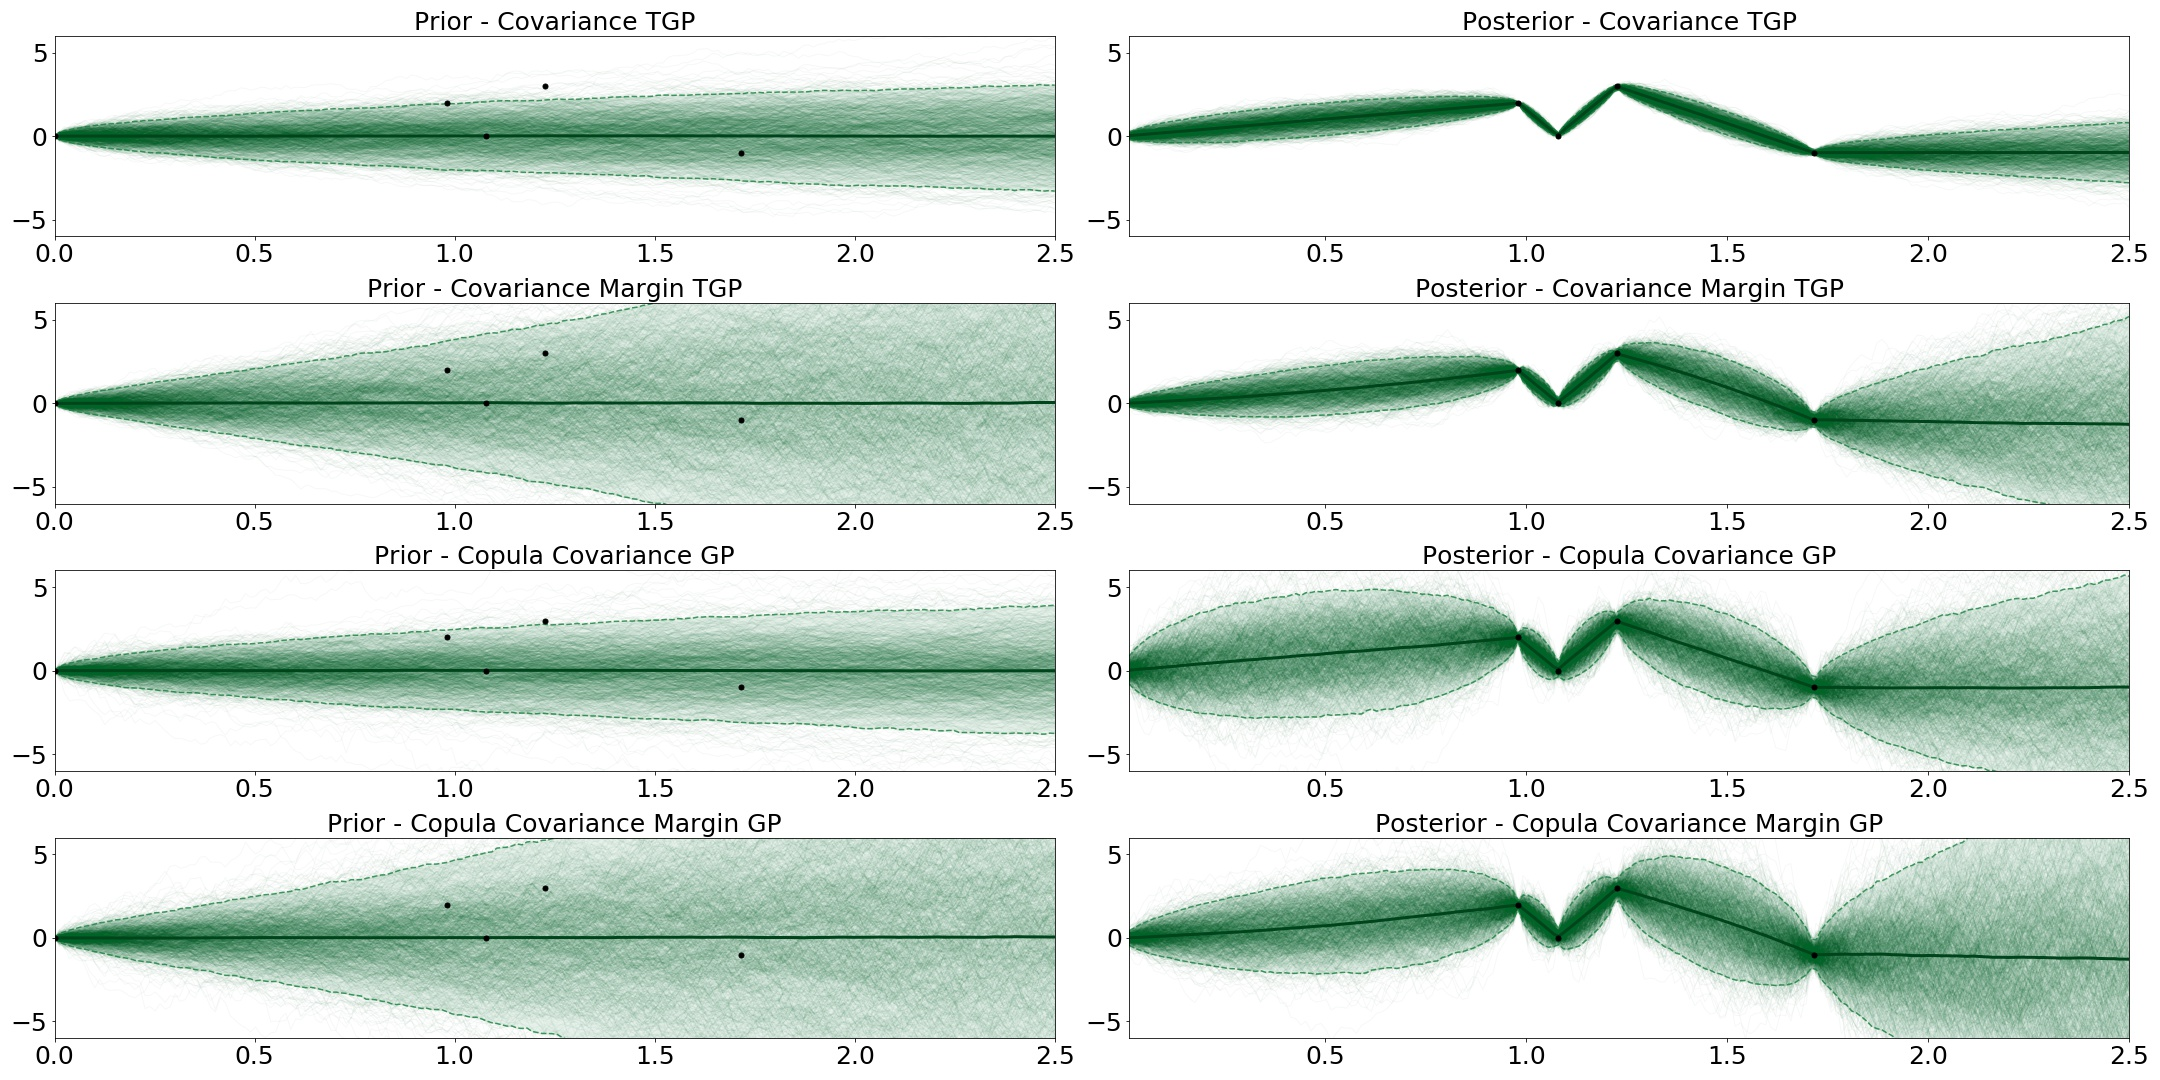
\includegraphics[width=0.9\textwidth]{tgp}
	\caption{Muestras de cuatro TGP: el primer y segundo ejemplos tienen cópula gaussiana, mientras que el tercero y cuarto tienen cópulas de \(t\) de Student.}
	\label{fig_tgp1}
\end{figure}


\section{Proceso Transportado Profundo}
\label{sec:computationtgp}
Tanto la generalidad como el cálculo factible del enfoque presentado basado en el transporte para la regresión no paramétrica nos motivan a definir modelos complejos inspirados en los avances recientes de la comunidad de aprendizaje profundo. Mediante la composición de transportes elementales (o \emph{capas}) podemos generar transportes más expresivos (o \emph{profundos}). En esta sección, explicaremos cómo construir dicha arquitectura, describiremos las propiedades que se heredan a través de la composición, para finalmente proponer familias de transportes que se pueden componer juntos y estudiar sus propiedades en el problema de regresión.



\subsection{Consistencia de un proceso transportado profundo}

En este artículo presentamos cuatro tipos de transportes, que pueden verse como \emph{capas} elementales para los modelos de regresión. Nuestro enfoque parte de una referencia de ruido blanco gaussiano \(f \sim \eta\), ya que es un proceso bien conocido con densidad explícita y métodos de muestreo eficientes. La primera capa determina la \emph{cópula} del proceso inducido (elíptica) mediante transportes elípticos. En el caso elíptico, es posible componerlo con un transporte de covarianza para determinar la correlación sobre el proceso estocástico inducido. Finalmente, en cualquier caso, podemos componer cualquier número de transportes marginales para definir una distribución marginal expresiva sobre el proceso estocástico inducido, como se muestra en el trabajo anterior \cite{cwgp}. Como vimos en las secciones anteriores, estas composiciones son lo suficientemente consistentes y expresivas como para incluir GP, GP alabeadas, procesos de Student-t, procesos elípticos y los que podríamos llamar \emph{procesos elípticos deformados}.


\subsection{Entrenamiento de un proceso transportado profundo}
Asumiendo \(T\#\eta = \pi\), donde \(T\) es una composición de \(k\) transportes, es decir \(T = T^{(k)} \circ ... \circ T^{(1)}\). Denotando \(\eta^{(0)}=\eta\) y asumiendo que cada \(\eta^{(j)}=T^{(j)}\#\eta^{(j-1)}\) es un proceso transportado con transportes finito dimensionales \(\{T_{\bft}^{(j)}\}_{j=1}^k\). Notemos que \(\eta^{(k)} = T\#\eta = \pi\), donde \(T_{\bft} = T_{\bft}^{(k)} \circ ... \circ T_{\bft}^{(1)}\) son transportes finito dimensionales con \(S_{\bft} = S_{\bft}^{(1)} \circ ... \circ S_{\bft}^{(k)}\). Como consecuencia, la composición de procesos transportados es un proceso transportado. En consecuencia, la NLL puede ser calculada como
\begin{align}
\label{eq:TGP_NLL2}
-\log \pi_{\bft}(\bfy|\theta) = -\log \eta_{\bft}(S_{\bft}(\bfy)) - \sum\nolimits_{j=1}^k \log |\nabla S_{\bft}^{(j)}(S_{\bft}^{[(j+1):k]}(\bfy))|,
\end{align}
donde \(S_{\bft}^{[j:k]}(\bfy) = S_{\bft}^{(j)} \circ ... \circ S_{\bft}^{(k)} (\bfy)\), con la convención \(S_{\bft}^{[(k+1):k]}(\bfy) = \bfy\). La fórmula anterior se basa en el cálculo de cada \(F_{\bft}^{(j)}(\bfz)= \log |\nabla S_{\bft}^{(j)}(\bfz)|\), que se puede calcular alternativamente como \(F_{\bft}^{(j)}(\bfz)=- \log |\nabla T_{\bft}^{(j)}(S_{\bft}^{(j)}(\bfz))|\), o, para el caso triangular y diagonal, como \(F_{\bft}^{(j)}(\bfz)=\sum_{i} \log \frac{\partial (S_{\bft})_i}{\partial y_i}(\bfz)\). El siguiente algoritmo calcula la NLL, sujeto a poder evaluar cada función \(F_{\bft}^{(j)}\) t \(S_{\bft}^{(j)}\).

\begin{algorithm}[!h]
	\caption{Calcula la NLL de un proceso transportado profundo}
	\label{algo1}
	\begin{algorithmic} 
		\Require Datos \((\bft,\bfy )\), transportes inversos \(T^{-1}_{\bft}(\bfz) = S_{\bft}^{(1)} \circ ... \circ S_{\bft}^{(k)}(\bfz)\) y \(F_{\bft}^{(j)}(\bfz)=\log |\nabla S_{\bft}^{(j)}(\bfz)|\).
		\Ensure  \(\mathcal{L} = -\log \pi_{\bft}(\bfy|\theta)\)
		\State \(\bfz \gets \bfy\), \(\mathcal{L} \gets 0\)
		\For{\( j \in k,...,1 \)}
		\State \(\mathcal{L} \gets \mathcal{L} - F_{\bft}^{(j)}(\bfz)\)
		\State \(\bfz \gets S_{\bft}^{(j)}(\bfz)\)
		\EndFor
		\State \(\mathcal{L} \gets \mathcal{L} - \log \eta_{\bft}(\bfz)\)
		\Return \(\mathcal{L}\)
	\end{algorithmic}
\end{algorithm}

\begin{remark}
	El algoritmo \ref{algo1} está basado en aplicar la regla de la cadena y el teorema de la función inversa sobre la composición de inversas \(S_{\bft} = S_{\bft}^{(1)} \circ ... \circ S_{\bft}^{(k)}\), entonces
	\begin{align}
	\nabla S_{\bft}(\bfy) &= \nabla S_{\bft}^{(1)}( S_{\bft}^{(2)} \circ ... \circ S_{\bft}^{(k)}) \nabla S_{\bft}^{(2)}( S_{\bft}^{(3)} \circ ... \circ S_{\bft}^{(k)}) .... \nabla S_{\bft}^{(k-1)}(S_{\bft}^{(k)}(\bfy))  \nabla S_{\bft}^{(k)}(\bfy),\\
	&= \nabla T_{\bft}^{(1)}( S_{\bft}^{(1)} \circ ... \circ S_{\bft}^{(k)})^{-1} \nabla T_{\bft}^{(2)}( S_{\bft}^{(2)} \circ ... \circ S_{\bft}^{(k)})^{-1} .... \nabla T_{\bft}^{(k)}(S_{\bft}^{(k)}(\bfy))^{-1}.
	\end{align}
\end{remark}

El algoritmo \ref{algo1} es computacionalmente eficiente en términos de uso mínimo de memoria (incluso la variable \(\bfz\) puede usar la misma memoria que \(\bfy\)), y se puede ejecutar en el menor tiempo posible llamando a cada función \(F_{\bft}^{(j)}\) y \(S_{\bft}^{(j)}\) solo una vez. Al implementar los cálculos de NLL en cualquier marco de tensor moderno, como PyTorch, es posible aplicar la diferenciación automática \cite{paszke2017automatic} para calcular la derivada de NLL con respecto a los parámetros. Además, este algoritmo es paralelizable en \(\theta\), lo que permite una evaluación eficiente de NLL para múltiples valores de \(\theta\) simultáneamente en arquitecturas como las GPU. Esta es una propiedad deseada para los métodos de optimización sin derivados, como la optimización de enjambres de partículas \cite{kennedy2010particle}, o los muestreadores de conjuntos MCMC \cite{goodman2010ensemble}. En los métodos de descenso de gradiente estocástico \cite{bottou2010large}, dado que en cada paso usamos un submuestreo de los datos, podemos aprovechar las arquitecturas basadas en GPU que se ejecutan en múltiples ejecuciones paralelas, para navegar mejor en el espacio de los modelos.


\subsection{Inferencia de un proceso transportado profundo}

Como la operación de composición conserva la triangularidad, asumimos que \(T^{(j)}\) son triangulares para \(j > l\), además de poder calcular la parte posterior de \(\eta^{(l)}\), es decir, calcular \(\eta_{\bfto|\bft}^{(l)}(\cdot|\bfx)\) para cualquier entrada \(\bfto\). Sin pérdida de generalidad, se puede suponer que \(l = 1\), ya que es posible colapsar por composición los transportes de \(l\) en uno solo. El siguiente algoritmo genera muestras de la distribución posterior \(\pi_{\bfto|\bft}(\bfyo|\bfy)\) bajo los supuestos anteriores.

\begin{algorithm}[!h]
	\caption{Generar muestras desde la posterior}
	\label{algo2}
	\begin{algorithmic} 
		\Require Observaciones \(\bfy \sim \pi_{\bft}\), nuevas entradas \(\bfto \in \calI^d, d \in \mathbb{N}\), número de muestras \(N \in \naturals\).
		\Ensure  \(\bfyo_i \sim \pi_{\bfto|\bft}(\bfyo|\bfy)\) para \(i=1,...,N\)
		\State \(\bfx \gets S_{\bft}^{[l+1:k]}(\bfy)\)
		\State \(R(\cdot) \gets P_{\bfto} \circ T_{\bft,\bfto}^{[l+1:k]}(\bfx, \cdot)\)
		\For{\( i \in 1,...,N \)}
		\State \(\bfxo_i \sim \eta_{\bfto|\bft}^{(l)}(\cdot|\bfx)\)
		\State \(\bfyo_i \leftarrow R(\bfxo_i)\)
		\EndFor
		\Return \(\{\bfyo_1,...,\bfyo_N\}\)
	\end{algorithmic}
\end{algorithm}

El algoritmo \ref{algo2} es paralelizable en \(N\), ya que la función \(R(\cdot)\) es la misma para todas las muestras, y por lo tanto nos permite obtener múltiples muestras simultáneamente de manera eficiente. Este puede ser utilizado a su vez para calcular momentos, cuantiles u otras estadísticas de forma empírica a través de Monte Carlo.

\subsection{Capa ruidosa}

Bajo la presencia de observaciones ruidosas, siguiendo la misma lógica que los GPs, warped GPs \cite{snelson2004warped} y los procesos Student-t \cite{shah2014student}, consideramos que el transporte de covarianza tiene un comportamiento especial. Sea \(k(t,s) = r(t,s) + \sigma_0\delta_{t,s}\), donde \(\delta\) es delta de Kronecker, \(\sigma_0\) es el parámetro que controla la intensidad del ruido y \(r(t,s)\) es la función de covarianza libre de ruido. Consideramos que las observaciones tienen ruido no correlacionado. Mientras que para el entrenamiento usamos \(k(t,s)\) en la fórmula de NLL, en la inferencia usamos \(k(t,s)\) en el paso hacia atrás (es decir, para el mapa inverso \(\bfx = T_{\bft }^{-1}(\bfy)\)), y en el paso hacia adelante (es decir, para impulsar la distribución de referencia) usamos \(r(t,s)\), en lugar de \(k(t,s)\) , para realizar una predicción de ruido libre.


\subsection{Sparse layer}
Mientras que los transportes marginales y de cópula se pueden evaluar de manera eficiente sin necesidad de datos de entrenamiento, los transportes de covarianza necesitan todos los datos \(\bfy\) para la inferencia de rendimiento. La complejidad computacional de la evaluación es \(\O(n^2)\) en memoria y \(\O(n^3)\) en tiempo, donde \(n=|\bfy|\). Las aproximaciones dispersas se usan ampliamente para resolver este problema en los GP \cite{quinonero2005unifying, snelson2006sparse, titsias2009variational}, y es natural definir un transporte \emph{sparse} como \(T_{\bfto}(\bfu) = \Sigma_{\ bfto\bfs}\Sigma_{\bfs\bfs}^{-1}\bfz + \chol(\Sigma_{\bfto\bfto} - \Sigma_{\bfto\bfs}\Sigma_{\bfs\bfs}^{ -1}\Sigma_{\bfto\bfs})\bfu\), donde \((\bfs,\bfz)\) son pseudodatos entrenables con \(|\bfs| = m < n\). El entrenamiento de pseudodatos sigue las mismas ideas que los GP dispersos, como las aproximaciones SoD y SoR \cite{quinonero2005unifying}, donde el costo computacional cae a \(\O(nm)\) en el espacio y \(\O(nm^2)\) a tiempo.


\section{Validación Experimental}
\label{sec:experimentstgp}

\comment{le cambiaria el nombre a algo asi como: 'aplicación' o ejemplo, porque como es algo ya establecido no deberia ser una validación}

Validamos nuestro enfoque con tres series de tiempo del mundo real, descritas a continuación:
\begin{enumerate}
	\item \textbf{Datos de manchas solares}: La serie temporal de manchas solares \cite{sunspots} corresponde al número anual de manchas solares entre 1700 y 2008, lo que da como resultado 309 puntos de datos, uno por año. Estas medidas son positivas y semiperiódicas, con un ciclo de alrededor de 11 años.
	\item \textbf{Datos de frecuencia cardíaca}: Esta es una serie temporal de frecuencia cardíaca de la base de datos MIT-BIH (ecg.mit.edu) \cite{glass2012theory}. Esta serie contiene 1800 mediciones positivas espaciadas uniformemente de la frecuencia cardíaca instantánea (en unidades de latidos por minuto) de un solo sujeto, que ocurren a intervalos de 0,5 segundos y muestran un patrón semiperiódico. Para problemas de rendimiento, tomamos una submuestra de 450 medidas en intervalos de 2,0 segundos.
	\item \textbf{Datos económicos}: Esta serie de tiempo corresponde al promedio trimestral \emph{3-Month Treasury Bill: Secondary Market Rate} \cite{tb3ms} entre el primer trimestre de 1959 y el tercer trimestre de 2009, es decir, 203 observaciones, una por trimestre. Sabemos de antemano que esta señal macroeconómica es el precio de los bonos libres de riesgo del gobierno estadounidense, que no pueden tomar valores negativos y pueden tener grandes desviaciones positivas.
\end{enumerate}

Debido a la naturaleza semiperiódica de la serie temporal, consideramos una mezcla espectral ruidosa con dos componentes kernel \(k_{SM}\) \cite{wilson2013gaussian} para el transporte de covarianza. Dado que las series de tiempo son positivas, usamos una deformación de Box-Cox desplazada \(\phi_{BC}\) \cite{rios2018learning} para el transporte marginal. Comparamos dos modelos: un GP distorsionado, con \(k_{SM}\) kernel y \(\phi_{BC}\) warping; y un TGP con un transporte de cópula Student-t, además de los transportes marginales y de covarianza descritos anteriormente.

Dejamos los GP estándar fuera del experimento ya que la suposición de gaussianidad viola la naturaleza de los conjuntos de datos, ya que tiene un poder predictivo más bajo que el WGP, como se muestra en \cite{rios2018learning, riostobar2019cwgp}. Para ilustrar este hecho, en la Fig. \ref{fig_sunspots} mostramos la parte posterior de tres modelos entrenados: GP en azul, WGP en verde y TGP en morado. Graficamos las observaciones (puntos negros), la media (línea continua), el intervalo de confianza de 95\textbf{\%} (línea discontinua) y 25 muestras (líneas borrosas). Observe cómo el GP falla al modelar la positividad y la amplitud correcta de los fenómenos.

\begin{figure}
	\centering
	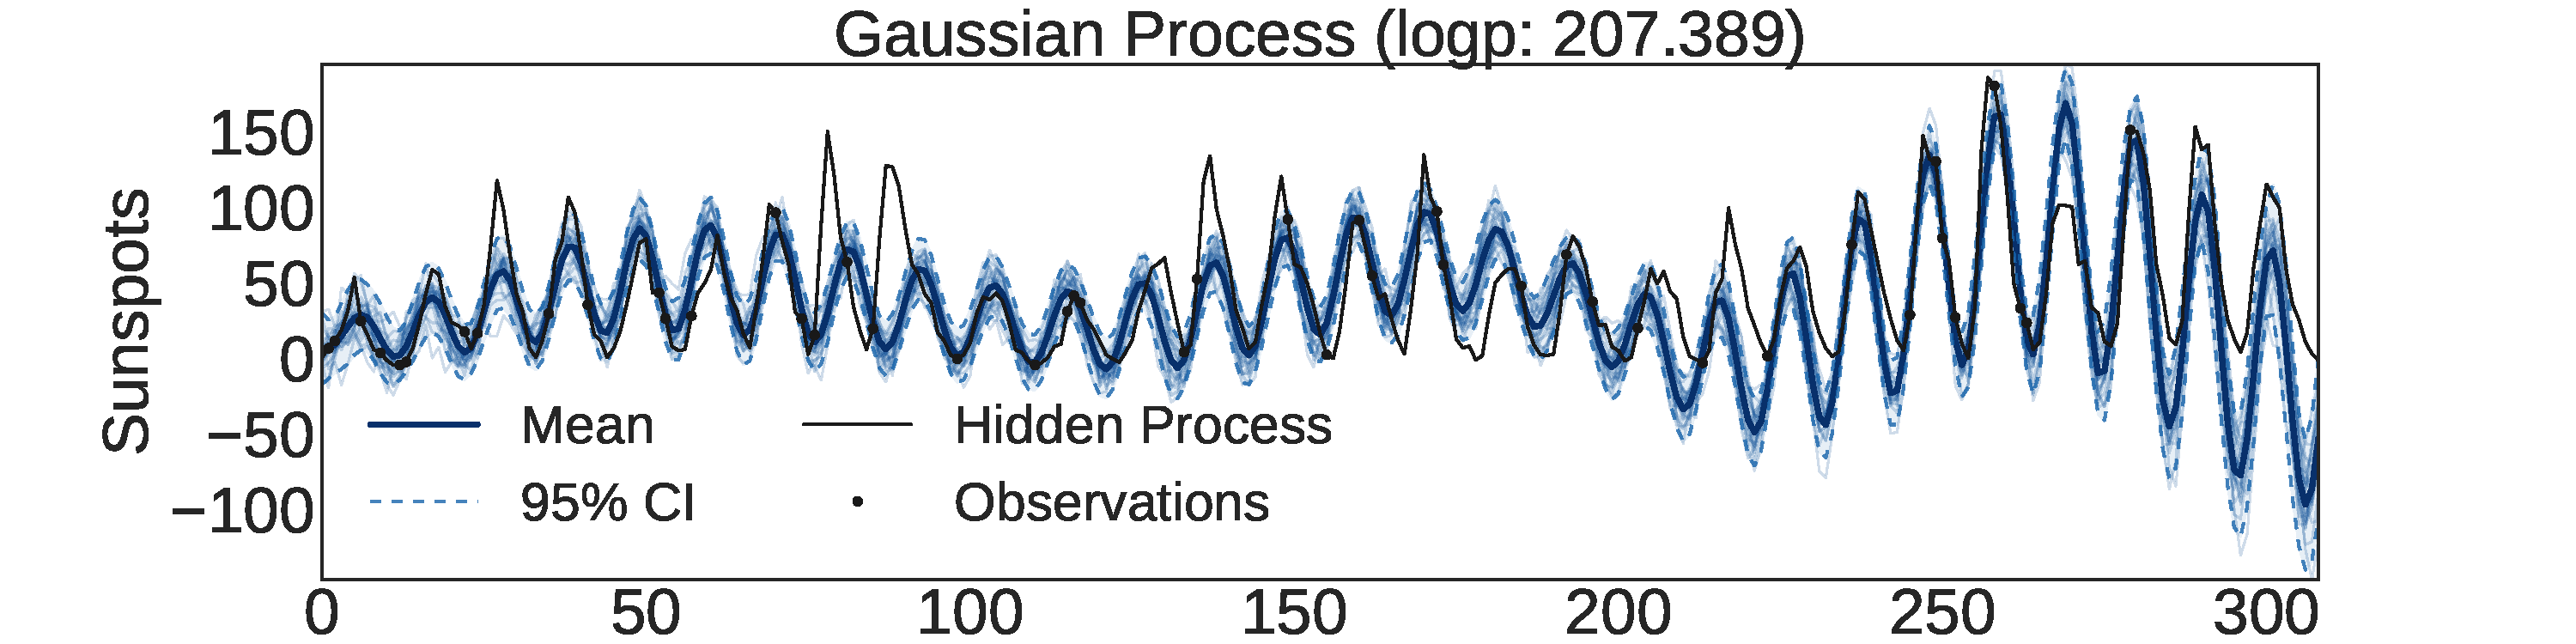
\includegraphics[width=0.7\textwidth]{example_sunspots_gp}
	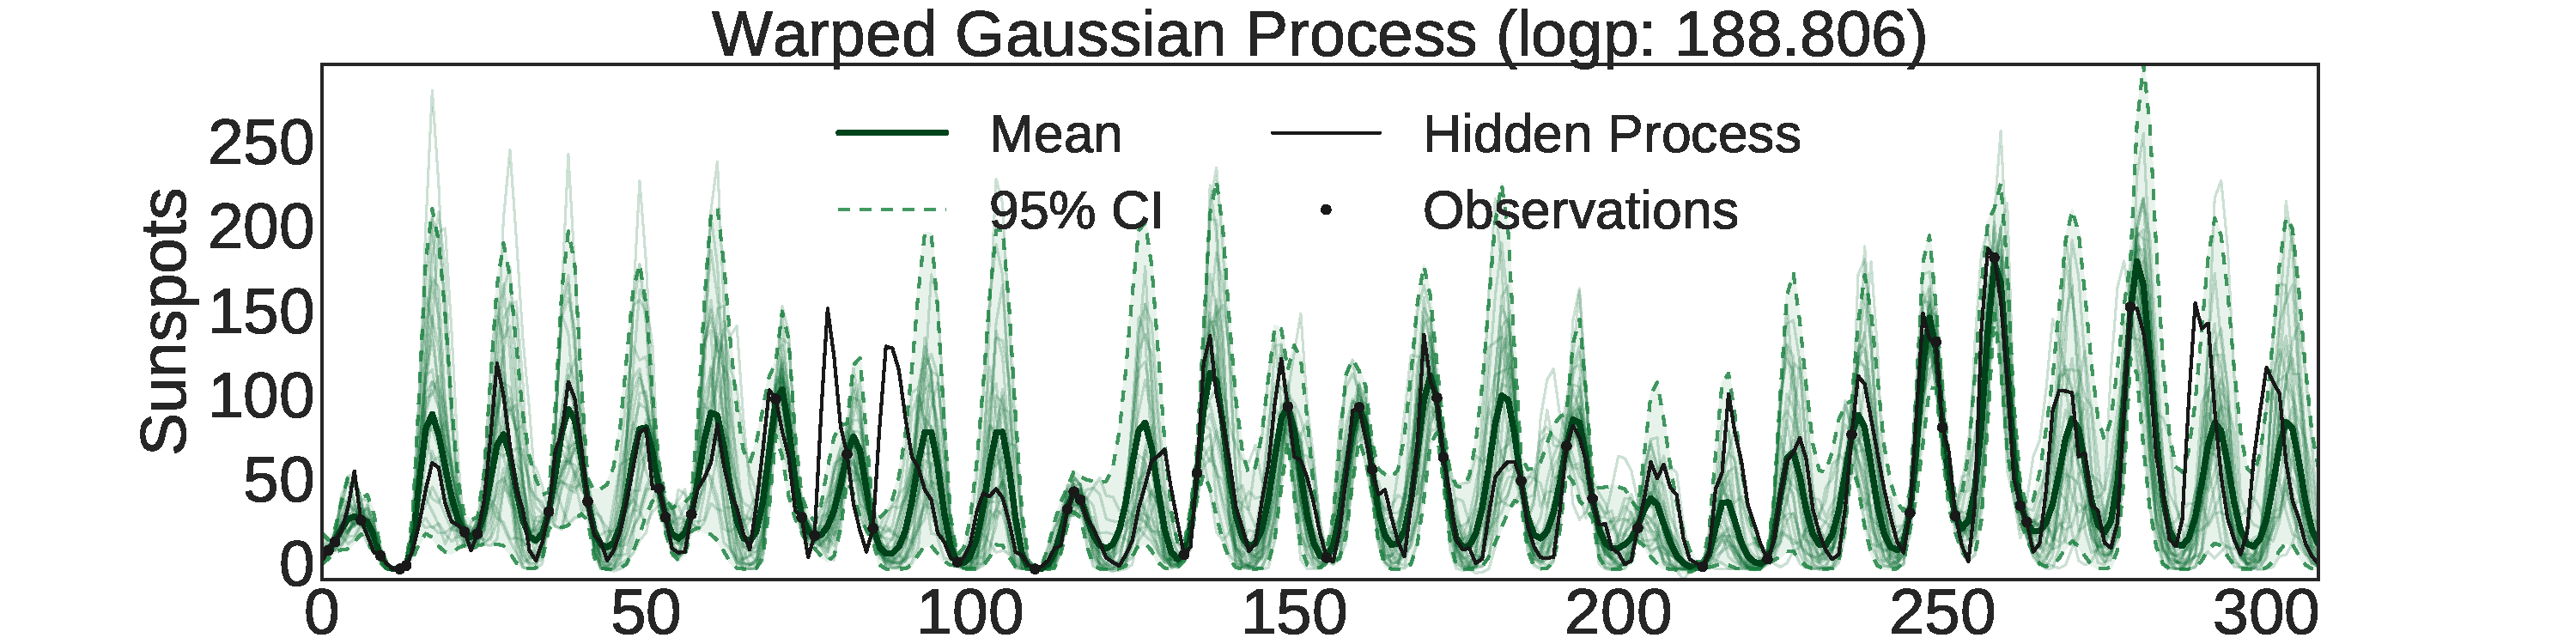
\includegraphics[width=0.7\textwidth]{example_sunspots_wgp}
	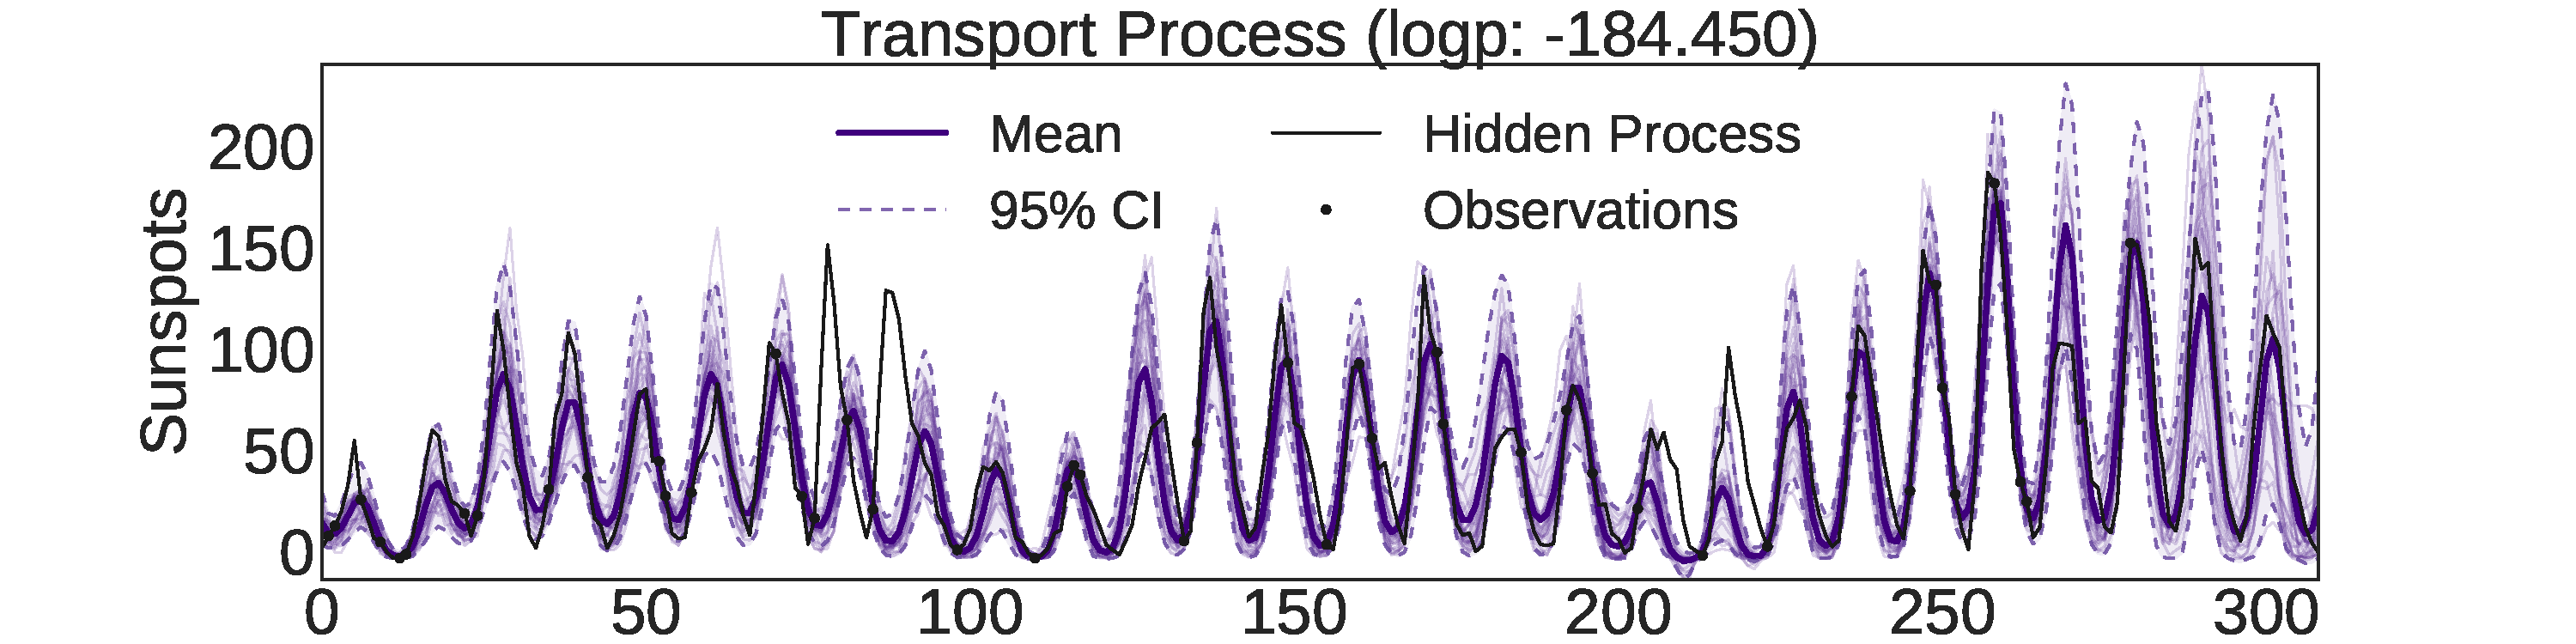
\includegraphics[width=0.7\textwidth]{example_sunspots_tgp}
	\caption{GP (azul), WGP (verde) y TGP (púrpura) sobre los datos de manchas solares.}
	\label{fig_sunspots}
\end{figure}


\begin{table}
	\centering
	\tiny
	\begin{tabular}{l|ll|ll|ll}
		\toprule
		{} & \multicolumn{2}{l}{Manchas Solares} & \multicolumn{2}{l}{Frecuencia Cardíaca} & \multicolumn{2}{l}{Económica} \\
		{} &                      WGP &                      TGP &                 WGP &                 TGP &                WGP &                TGP \\
		\midrule
		MAE &       25.266 \(\pm\) 4.607 &       24.710 \(\pm\) 4.271 &   2.965 \(\pm\) 0.827 &   2.907 \(\pm\) 0.715 &  1.132 \(\pm\) 0.260 &  1.111 \(\pm\) 0.215 \\
		EAE &       30.166 \(\pm\) 4.374 &       29.649 \(\pm\) 4.168 &   3.431 \(\pm\) 0.732 &   3.388 \(\pm\) 0.660 &  1.392 \(\pm\) 0.235 &  1.380 \(\pm\) 0.206 \\
		MSE &  1,306.253 \(\pm\) 560.496 &  1,223.257 \(\pm\) 421.385 &  16.405 \(\pm\) 8.809 &  15.740 \(\pm\) 7.619 &  3.002 \(\pm\) 1.643 &  2.860 \(\pm\) 1.311 \\
		ESE &  1,889.318 \(\pm\) 633.325 &  1,796.989 \(\pm\) 514.193 &  21.963 \(\pm\) 8.524 &  21.554 \(\pm\) 8.213 &  4.376 \(\pm\) 1.725 &  4.272 \(\pm\) 1.424 \\
		\bottomrule
	\end{tabular}
	\vspace{0.5em}
	\caption{WGP and TGP results over Sunspots, Heart and Economic datasets.}
	\label{tab:table_results} 
\end{table}


El experimento se implementó en una biblioteca basada en Python llamada \emph{tpy: Transport Processes in Python}\cite{tpy}, con un backend de PyTorch para compatibilidad con GPU y diferenciación automática \cite{paszke2017automatic}. El entrenamiento se realizó minimizando el NLL de eq.~\eqref{eq:TGP_NLL2}, a través de un método rprop de mini lotes estocásticos \cite{riedmiller1993direct}, para luego terminar con iteraciones no estocásticas.

En cada experimento, seleccionamos al azar (uniformemente) 15\text{\%} de los datos para entrenamiento y los 85\text{\%} restantes para validación. Dados los puntos de datos de validación \(\{y_i\}_{i=1}^n\), para cada modelo generamos \(S\) muestras \(\{y_i^{(k)}\}_{i=1}^n \) para \(k=1,...,S\), y luego calculamos cuatro índices de rendimiento: el error cuadrático medio como \(\text{MSE} = \frac{1}{n}\sum\limits_{i=1 }^{n}\left(y_{i} - \frac{1}{S}\sum_{k=1}^{S}y_i^{(k)}\right)^2\), el error absoluto medio como \(\text{MAE} = \frac{1}{n}\sum\limits_{i=1}^{n}|y_{i} - \frac{1}{S}\sum_{k=1} ^{S}y_i^{(k)}|\), el error cuadrado esperado como \(\text{ESE} = \frac{1}{n}\sum\limits_{i=1}^{n}\frac{ 1}{S}\sum_{k=1}^{S}(y_{i} - y_{i}^{(k)})^2\), y el error absoluto esperado como \(\text{EAE} = \frac{1}{n}\sum\limits_{i=1}^{n}\frac{1}{S}\sum_{k=1}^{S}|y_{i} - y_{i} ^{(k)}|\). Repetimos cada experimento 100 veces. Los resultados de todos estos experimentos se resumen en la Tabla 1, que muestra cada media y desviación estándar. Consistentemente, el TGP propuesto tiene un mejor rendimiento que la alternativa de warped GP, para cada conjunto de datos e índice de evaluación.

\comment{parrafo: concluir y aterrizar los conceptos mencionados, generar una pequeña discusión sobre aplicaciones, limitantes y demasese. motivar la lectura tanto de otros capitulos como de demás literatura}
	%!TEX root = main.tex

\chapter{Marketing Mix Modeling}

\begin{chapquote}{John Wanamaker}
	``"La mitad del dinero que me gasto en publicidad es un desperdicio: el problema es que no sé qué mitad es.''
\end{chapquote}

\comment{contextualizar con otras partes del libro, mencionar la motivación y de por que esta este capitulo en el libro.}

\comment{parrafo: agregar resumen del capitulo y los temas que se mencionan}

El modelado de mezcla de marketing, conocido como (\emph{marketing mix modeling} en inglés denotado como MMM) constituye una técnica de modelado destinada a discernir las conexiones entre la inversión en marketing en diversos canales y los logros alcanzados, ya sea en términos de tráfico web, ventas, captación de clientes u otros idicadores clave de rendimiento (\emph{key performance indicator} en inglés denotado como KPI). El enfoque del MMM se basa en el análisis de datos históricos y la aplicación de métodos de regresión para desentrañar la contribución de cada canal en relación con los KPI.

En este capítulo, se expondrán y detallarán los aspectos fundamentales de nuestra metodología en el ámbito del MMM. Se ofrecerá una panorámica del modelo básico empleado, seguido de una descripción minuciosa con el enfoque de aprendizaje automático bayesiano.

\section{Introducción al MMM}

La revolución de los grandes datos de los últimos años se deriva del aumento en la cantidad de datos disponibles, la expansión del poder de cómputo y los avances en los algoritmos de aprendizaje profundo utilizados por los profesionales. A la luz de la forma en que se ha desarrollado el campo, puede parecer que cualquier problema que involucre datos puede resolverse con éxito mediante una aplicación de procesamiento numérico suficiente.

La realidad, sin embargo, es que para una gran clase de problemas, la cantidad de datos disponibles es demasiado pequeña para que las técnicas de aprendizaje profundo sean aplicables. Esta es la categoría en la que cae MMM: los volúmenes de datos sobre gastos de marketing y ventas u otras métricas comerciales relevantes que están disponibles al construir un MMM están lejos de los utilizados en el ámbito de las grandes empresas de big data. Esto es inherente a los problemas de regresión de series temporales, donde el horizonte temporal de los datos disponibles es cercano a los tres años en un caso ideal, es decir, menos de doscientos puntos temporales semanales.

El gran desafío en MMM es extraer la mayor cantidad de inteligencia posible de pequeños conjuntos de datos para brindar una solución que funcione para la mayoría de los anunciantes. Logramos esto mediante el uso de un enfoque bayesiano de MMM, que es diferente en varios aspectos del marco clásico basado en la regresión.


\section{Input Data}

Comenzamos con un conjunto de datos indexados en el tiempo (generalmente ventas) \(\mathcal{D} = \{(t_1, y_1), \dotsc, (t_n, y_n)\}\) y variables explicativas indexadas en el tiempo.

\begin{figure}[h]
	\centering
	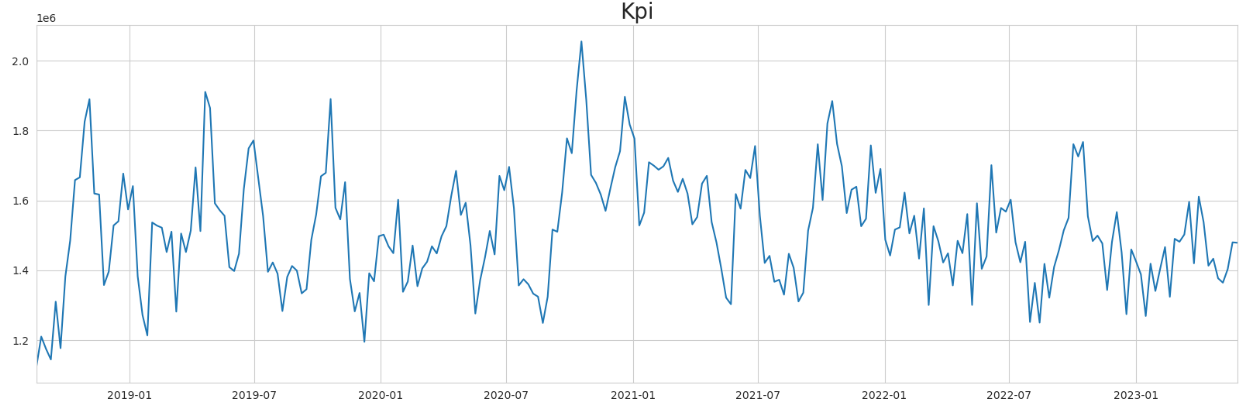
\includegraphics[width=0.9\textwidth]{KPI}
	\caption{Ejemplo de un serie de KPI.}\label{KPI}
\end{figure}

La cantidad mínima de datos necesaria para estimar un modelo de mezcla de marketing es una variable dependiente (generalmente ventas, denotadas por \(y_0, \dotsc y_t\)), y series de inversión para una cantidad de medios, denotadas \(x_0^m, \dotsc, x_t^m\), y \(m \in M\) es el conjunto de medios. Siempre que hablamos de series asumimos que son series temporales, indexadas en el tiempo.


\begin{figure}[h]
	\centering
	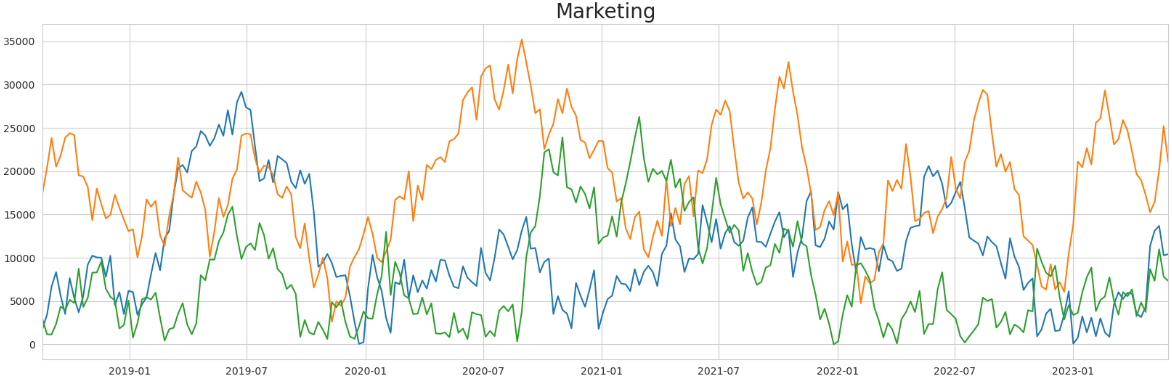
\includegraphics[width=0.9\textwidth]{Marketing}
	\caption{Ejemplo de series de marketing.}\label{Marketing}
\end{figure}

Otros datos opcionales que se pueden considerar son la inversión de la competencia, las inversiones no controlables, el precio, la distribución, las variables macroeconómicas, las fechas especiales, etc. Nuevamente, estas deben ser series de tiempo.

Sin pérdida de generalidad, cada serie se reducirá en el intervalo \([-1, 1]\) para trabajar. Algunas series se reducirán utilizando el cuantil 95 ya que deben ser no negativas (como gasto o ventas), mientras que otras se normalizarán (centradas y normalizadas por la desviación estándar), como precio, distribución u otras.

\subsection{MMM}


Para simplificar, supondremos aquí que la variable objetivo corresponde a las ventas, aunque la estructura básica del modelo se puede aplicar a una variedad de otras métricas comerciales de interés (como visitas a tiendas o un sitio web, oportunidades de ventas o el número de clientes captados de los competidores) con sólo modificaciones menores. Para cada período de tiempo $t$, las ventas ($S_t$) se descomponen como el producto entre un componente de tendencia, compuesta por una componente incremental y una componente base, y una componente de estacionalidad: \medskip
\begin{equation*}
\tikzmark{s} S_t ~~~=~~~ \tikzmark{t} T_t \, \cdot \, F_t \tikzmark{p}.
\begin{tikzpicture}[overlay,remember picture]
\node (S1) [left of = s, node distance = 4.5em, yshift=0.5em]{\footnotesize ventas};
\node (S2) [left of = s, node distance = 0em, yshift=0.25em]{};
\draw[->, in=180, out=350] (S1.east) to (S2.west);
\node (T1) [left of = t, node distance = 4.5em, yshift=1.5em]{\footnotesize tendencia};
\node (T2) [left of = t, node distance = 0em, yshift=0.8em]{};
\draw[->, in=150, out=350] (T1.east) to (T2.west);
\node (P1) [right of = p, node distance = 4.5em, yshift=1.5em]{\footnotesize factor};
\node (P2) [right of = p, node distance = -0.5em, yshift=0.8em]{};
\draw[->, in=45, out=210] (P1.west) to (P2.east);
\end{tikzpicture}
\end{equation*}

La componente de tendencia de las ventas $T_t$ se da a su vez como la suma de dos componentes de ventas incrementales más las ventas bases:\medskip
\begin{equation*}
\tikzmark{t} T_t ~~~=~~~ \tikzmark{im} I^\calM_t ~+~ I^\calC_t \tikzmark{ic} ~+~ B_t \tikzmark{b}.
\begin{tikzpicture}[overlay,remember picture]
\node (E1) [left of = im, node distance = 4.5em, yshift=1.5em]{\footnotesize marketing inc.};
\node (E2) [left of = im, node distance = 0em, yshift=0.8em]{};
\draw[->, in=150, out=350] (E1.east) to (E2.west);
\node (T1) [right of = ic, node distance = 5.5em, yshift=1.3em]{\footnotesize no controlable inc.};
\node (T2) [right of = ic, node distance = 0em, yshift=0.8em]{};
\draw[->, in=25, out=200] (T1.west) to (T2.east);
\node (B1) [right of = b, node distance = 4.5em, yshift=0.5em]{\footnotesize base};
\node (B2) [right of = b, node distance = 0em, yshift=0.25em]{};
\draw[->, in=0, out=180] (B1.west) to (B2.east);
\end{tikzpicture}
\end{equation*}

Los componentes incrementales $I_t = I^\calM_t + I^\calC_t$ modelan ventas que resultan, respectivamente, directamente de acciones de marketing y de acciones no controladas por el cliente. En la versión más básica del modelo, $I^\calM_t$ se modela como una suma sobre las ventas que son atribuibles directamente al gasto en cada uno de los diferentes canales de medios,
\begin{equation}\label{incremental}
\tikzmark{i} I^\calM_t ~~~=~~~ \sum_{m=1}^{\tikzmark{mtot} M} A^{(m)}_t \tikzmark{a}.
\begin{tikzpicture}[overlay,remember picture]
% \node (I1) [left of = i, node distance = 4.5em, yshift=0.6em]{\footnotesize incremental};
% \node (I2) [left of = i, node distance = 0em, yshift=0.25em]{};
% \draw[->, in=180, out=350] (I1.east) to (I2.west);
\node (M1) [left of = mtot, node distance = 9.5em, yshift=0.5em]{\footnotesize número de medios};
\node (M2) [left of = mtot, node distance = 0em, yshift=0.2em]{};
\draw[->, in=185, out=0] (M1.east) to (M2.west);
\node (A1) [right of = a, node distance = 9.5em, yshift=0.85em]{\footnotesize adstock del medio $m$};
\node (A2) [right of = a, node distance = 0em, yshift=0.8em]{};
\draw[->, in=10, out=185] (A1.west) to (A2.east);
\end{tikzpicture}
\end{equation}

El incremental no controlable $I^\calC_t$ se modela de manera similar. La componente de factor $F_t$ tiene un patrón cíclico y debe considerarse como un factor multiplicativo que oscila alrededor de $1$ para representar los diversos efectos estacionales a lo largo de múltiples periodicidades (semanales, mensuales, anuales) que se estiman por separado; este componente también tiene en cuenta campañas o eventos especiales únicos. Toda esta notación nos permite escribir nuestro modelo de una manera más clara como
\[f_t = (I_t + B_t) (1 + V_t).\]

Cada término tiene un significado distinto: en el momento \(t\), la componente incremental \(I_t\) representa el efecto de marketing (y otros efectos aditivos), la componente base \(B_t\) representa las ventas no directamente atribuibles a \( I_t\), y \(V_t\) representa las variaciones dadas por efectos temporales y otros efectos multiplicativos. Aclaramos que \(I_t\) y \(V_t\) son paramétricos y dependen de los datos de entrada (gastos de marketing, variables económicas, estacionalidades, precio, distribución, etc.), mientras que \(B_t\) no es paramétrico.

Ahora definimos varias cantidades de interés para el modelo:
\begin{itemize}
	\item La \emph{variación} es simplemente \(V_t\).
	\item El \emph{factor} se define como \(F_t = 1+V_t\).
	\item La \emph{tendencia} se define como \(T_t = I_t + B_t = \frac{f_t}{1+V_t}\).
	\item El término \emph{aditivo} se define como \(D_t = f_t - T_t = T_t V_t\).
	\item La componente \emph{explicado} se define como \(E_t = I_t (1 + V_t)\).
	\item La componente \emph{no explicado} se define como \(U_t = B_t (1 + V_t)\).
\end{itemize}

A continuación se expone un diagrama de un MMM básico.
\begin{figure}[h]
	\centering
	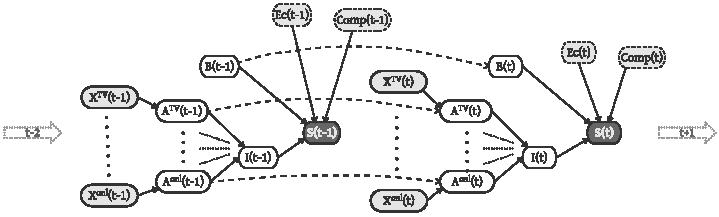
\includegraphics[width=\textwidth]{MMM.pdf}
	\caption{El MMM básico. Por ejemplo, las variables de stock publicitario $A^{\rm TV}(t),\dotsc,A^{\rm online}(t)$ dependen del nivel de inversión en los medios asociados en el período dado, $X^ {\rm TV}(t),\dotsc,X^{\rm online}(t)$, y en los niveles de acciones publicitarias del período anterior. Los detalles de esta dependencia se especifican como una propiedad del nodo adstock. En esta red también añadimos dependencia de las ventas $S\hspace{-0.15ex}(t)$ de un conjunto de variables económicas y de información sobre la competencia, ${\rm Ec}(t)$ y ${\rm Comp}(t)$.}\label{MMM-DBN}
\end{figure}

\subsection{Adstocks}
\label{subsec:adstocks}

\textit{Adstock} aquí se refiere al efecto agregado (medido como ventas) de los esfuerzos de marketing en los períodos actuales y pasados en un canal de medios determinado (en una versión más general del modelo, los anuncios de diferentes puntos de contacto de medios se pueden combinar en cualquier otra forma para modelar los efectos multiplicadores no lineales resultantes de acciones en diferentes medios). Al modelar la evolución del stock de anuncios publicitarios, se deben considerar tres aspectos: los efectos retardados o rezagados de las acciones publicitarias, la disminución de estos efectos a lo largo del tiempo y el efecto de saturación al que está sujeto el gasto en marketing. La dinámica básica de las acciones publicitarias en nuestro modelo implica, por lo tanto, una combinación entre los efectos de la publicidad en el período actual y en el pasado.


El adstock es, en palabras simples, el efecto que ha tenido una inversión a lo largo del tiempo. Construimos este efecto de la siguiente manera: primero definimos una función \(H\) en forma de S, llamada \textit{saturación}, usando dos parámetros \(u \in (0,1)\) y \(b > 0 \) (el punto de semisaturación y un parámetro de forma), de la siguiente manera:
\[ H_{ u,b }(x) = \frac{ x^b }{ u^b + x^b }. \]

Si \(x\) es un valor de gasto, \(H(x)\) modela la saturación de dicho gasto. Claramente tenemos que \( H(x) \in [0,1) \) y \(H(x) \to 1\) como \(x \to \infty\). \(u\) se llama semisaturación porque \(H(u) = 1/2\) (recuerde que la inversión se reduce, por lo que para recuperar \(u\) en la escala original simplemente multiplicamos \(u\) por la escala de esa serie).

\begin{figure}
	\centering
	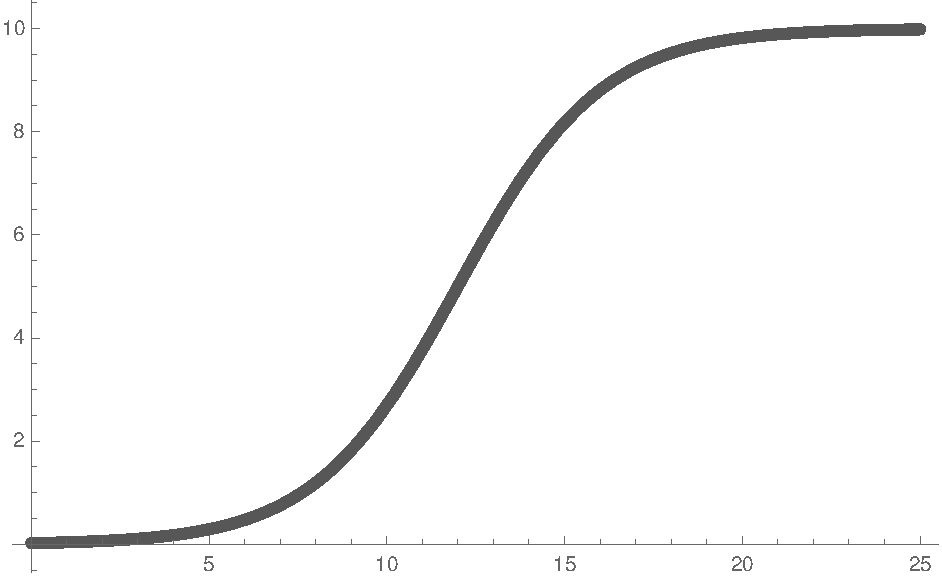
\includegraphics[width=0.52\textwidth]{logistic.pdf}
	\caption{Función sigmoidea típica \(H_m\). Depende de un conjunto de parámetros que controlan las principales características de su forma: el nivel de saturación (aquí alrededor de 10), el nivel de inversión en el que se alcanza la saturación (aquí alrededor de 22) y el punto donde comienzan los rendimientos decrecientes (es decir, donde la curva cambia de convexa a cóncava, aquí alrededor de 12)}
	\label{logística}
\end{figure}

Agregamos otro parámetro \(c\), el carry-cap, para modelar el efecto actual de un gasto a la vez. Entonces, en el momento \(s\) y la inversión \(x_s\), \(cH(x_s)\) modela el impacto en el momento \(s\) de la inversión saturada. Aunque técnicamente tenemos que \(c > 0\), a continuación especificamos que (y por qué) \(c \in (0,1)\).

Para modelar el efecto que ha tenido el gasto en el tiempo consideramos un retraso \(p\) en el tiempo (perdón por la redundancia) que afecta a los términos \(cH(x_s)\) en el tiempo. En detalle, \(p\) es una distribución binomial negativa\footnote{Esta variable aleatoria modela la probabilidad de obtener \(k\) éxitos al lanzar una moneda con probabilidad \(d\) de éxito dado que \(r\) ( no aleatorios) deben ocurrir fallas.}, uno versátil que nos permite modelar muchas formas de retraso. Dicha distribución está definida por dos parámetros \(d \in [0,1]\), \(r_l \in \naturals\), llamados decay y r-lag, que son la probabilidad de la moneda y la moda de la binomial negativa . La media de \(p\) viene dada por \(r = (1 - d) r_l / d + 1 \) y la distribución es:
\[ p(s) = \frac{ \Gamma(s + r) }{ s! \Gamma(r) } (1 - d)^{r} d^s. \]
Un valor más bajo de \(d\) implicará un retraso más rápido, ya que una menor probabilidad de éxito implicará acumular los fallos corregidos (aquí \(r\)) rápidamente. $r_l$ es la semana/mes donde un pulso de inversión alcanza su efecto máximo.


Juntando todo esto, para una serie de gastos \(x_0, \dotsc, x_t\) la función adstock para un medio \(m\) es una convolución en el tiempo entre la curva \(cH\) y el retraso \(p \):
\[ A(x_0^m, \dotsc, x_t^m) = \sum_{s=0}^t p(t-s) c H(x_s^m). \]
Un pequeño detalle a tener en cuenta es este: los datos tienen un tiempo de inicio, y no es posible tener datos antes de ese tiempo. Incluimos entonces otro término, un ``gasto en tiempo pasado'', denotado \(x_{-1}^m\) y denominado init-control, que pretende representar todo el gasto realizado antes de la primera vez de los datos. Este control de inicio también está saturado y complicado con \(p\). Por lo tanto, la función adstock se modifica para
\[ A(x_0^m, \dotsc, x_t^m) = \sum_{s=0}^t p(t-s) cH(x_s^m) + [1 - F_p(t+1)] cH(x_{- 1}^m), \]
donde \(F_p\) es la distribución acumulada de \(p\). Para una serie de gasto \((x_0^m, \dotsc, x_t^m)\) los parámetros \(c, u, b, d, r, x_{-1}\) deben ser entrenados para dicho \(m\).

La curva de descomposición $p_m$ se estima por separado para cada medio y modela la tasa a la que el efecto de una acción de marketing determinada en ese medio decae con el tiempo. $H_m$, por otro lado, es una función de forma sigmoidea que modela el efecto de saturación del gasto en un medio dado (ver Figura \ref{logística}). Esta curva de saturación se estima por separado para cada medio.

Dado que todas las inversiones deben modelarse como acciones publicitarias, también incluimos un parámetro de escala \(\alpha\) para entrenar, que modela el impacto de todas las acciones publicitarias de la siguiente manera:
\[ I_t^M = \alpha \sum_{m \in M} A(x_0^m, \dotsc, x_t^m). \]
Tenga en cuenta que \(\alpha\) multiplica todos los carry-caps, por lo que normalizamos todos los carry-caps a \([0,1]\) (y suman 1). Por lo general, se agrega una serie de stock publicitario (es decir, como una suma) al incremental. El efecto incremental es la suma de todos los incrementales, es decir \( I_t = I_t^M + I_t^{M'} + I_t^{M''} + \dotsb, \) donde los \(M\) posteriores son diferentes conjuntos de datos.


\subsection{Saturaciones}

Algunas series, como la económica, la de precios, la de distribución o las de valores atípicos, se pueden modelar mediante saturaciones. Actualmente consideramos cuatro efectos de saturación donde, independientemente del método, se debe entrenar un peso \(w\) y una escala \(\alpha\).
\begin{enumerate}
	\item Saturación por defecto: \(E(z_t) = \alpha \tanh(w z_t)\),
	\item Saturación lineal: \(E(z_t) = \alpha w z_t\),
	\item ``Uno más'' saturación: \(E(z_t) = 1 + \alpha \tanh(w z_t)\),
	\item ``Uno más'' saturación lineal: \(E(z_t) = 1 + \alpha w z_t\),
\end{enumerate}
Los dos primeros se suelen sumar al incremental. Los dos últimos se multiplican por el factor.

\subsection{Estacionalidad}

Un efecto particular que consideramos (multiplicado al factor actual) es el efecto estacional. Intentamos estimar una suma de senos y cosenos donde los periodos son las divisiones habituales de un año: un año entero, un semestre, un cuatrimestre, un trimestre, un bimestre y un mes. El efecto se define como
\[ Es(t) = 1 + \alpha \sum_{p\in P} c^1_p \sin\left(\frac{2\pi t}{p \varepsilon}\right) + c^2_p \cos \left(\frac{2\pi t}{p \varepsilon}\right),\]
donde \(P\) es el conjunto de periodos y \(\varepsilon \sim 1\) es un pequeño jitter en el caso semanal, pero igual a \(1\) en el caso mensual. Se deben entrenar los parámetros \(\varepsilon\) y \(c^1_p, c^2_p\), para todos los períodos.

\section{MMM as TGP}

Nuestro modelo es una regresión de la forma de un Proceso Gaussiano de Transporte (TGP) denotado \(f \sim \mathcal{TGP}(h, k)\), donde \(h\) es un transporte marginal y \(k\) un kernel de covarianza. A continuación explicamos cómo se eligen estas funciones \(h\) y \(k\) para dar forma al modelo final.

Observamos que dado que este es un problema de regresión, nuestro objetivo es encontrar el mejor predictor \(f\) tal que \(f\) esté cerca de los puntos de datos \(y\).

\subsection{Base}

Nuestra descripción hasta ahora ha sido puramente determinista, pero en realidad también debemos considerar la incertidumbre sobre lo que no podemos observar ni medir. Para ello añadimos dos componentes estocásticos diferentes. El primero es un vector de componentes base que pretende representar ventas base aleatorias.

El kernel de covarianza \(k\) determina la componente no paramétrico del modelo, que llamamos base. Este transporte de covarianza con el ruido viene dado por
\begin{align*}
k(s, t)	&= (1-\sigma) r(s, t) + \sigma \delta(s, t),\\
r(s, t)	&= \mathrm{SE}_{\ell_l}(s, t) \; \mathrm{SE}_{\ell_s}(s, t),\\
\mathrm{SE}_{\ell}(s, t) &= \exp\left( -\left(\frac{s-t}{100 \; \ell}\right)^2 \right),
\end{align*}
donde \(\sigma \in (0, 1)\) es la escala de ruido, \(\ell_l \in (0, 1)\) y \(\ell_s \in (0, 1)\) son largas y escalas de longitud corta, y \(\delta\) es el delta de Kronecker. Especificamos que \(\ell_s < \ell_l\).

Después de esto, consideramos el transporte marginal \( h_R(t, x) = \alpha \relu(2 + x) \). La razón para hacer esto es ``mover'' el proceso gaussiano generado por \(k\) lejos de \(0\), dejando solo alrededor de \(2\%\) de la masa debajo de \(0\). El \(\relu\) luego concentra este \(2\%\) de masa en \(0\). Esto da como resultado un TGP con distribuciones marginales gaussianas rectificadas (de ahí el subíndice \(R\)) y, por ahora, el TGP tiene la forma \( f \sim \mathcal{TGP}(h_R, k) \). Se deben entrenar los hiperparámetros $\sigma$, $\ell_l$, $\ell_s$ y $\alpha$.

\subsection{Noise}
Tenga en cuenta que el transporte de covarianza dado por \(k\) tiene ruido, dado por el delta de Kronecker. Podemos hacer la distinción entre un modelo ruidoso y uno silencioso, y simplemente denotar la predicción ruidosa con un superíndice como
\[f^{\mathrm{(n)}}_t = (I_t + B^{\mathrm{(n)}}_t) (1 + V_t).\]
Con esto, la componente de ruido es \(N_t = f_t^{\mathrm{(n)}} - f_t = (B^{\mathrm{(n)}}_t - B_t) (1 + V_t)\). En aras de la exhaustividad también podemos definir
\begin{itemize}
	\item The \emph{base ruidoso} as \(B^{\mathrm{(n)}}_t = B_t + \frac{N_t}{1 + V_t}\).
	\item The \emph{inexplicable ruidoso} as \(U^{\mathrm{(n)}}_t = U_t + N_t = B^{\mathrm{(n)}}_t (1 + V_t)\).
\end{itemize}
Finalmente, dado que \(y_t\) denota los datos observados (la variable a explicar), podemos definir la componente residual como \(R_t = f^{\mathrm{(o)}}_t - f_t = y_t - f_t\), donde el superíndice significa \emph{observado}. Especificamos que \( f^{\mathrm{(o)}}_t \stackrel{\mathrm{d}}{=} f^{\mathrm{(n)}}_t \), es decir, la predicción observada y la predicción ruidosa comparten la misma ley de probabilidad, pero es la posterior de la predicción observada la que coincide con los datos en sus tiempos asociados.

Todas las definiciones anteriores nos dan buenas formas diferentes de escribir y hablar sobre el modelo, como
\begin{align*}
f_t					&= (I_t + B_t) (1 + V_t) = T_t + A_t = E_t + U_t,\\
f_t^{\mathrm{(n)}}	&= (I_t + B^\mathrm{(n)}_t) (1 + V_t) = E_t + U_t + N_t,
\end{align*}
es decir, ``la predicción es tendencia más aditivo, pero también es explicado más no explicado''.

\subsection{Incremental}

El segundo y principal componente de nuestro modelo se llama incremental, una componente paramétrica que modela todos los efectos directos sobre la variable dependiente. Dadas algunas variables explicativas indexadas en el tiempo \(S_1, \dotsc, S_n\), la componente incremental viene dado por una función positiva \(I(t, S_1, \dotsc, S_n)\), con el transporte marginal asociado dado por \(h_I(t, x) = I_t + x\), donde \(I_t\) es el incremental en el tiempo \(t\).

Con esto, por ahora el modelo sigue la relación \(f \sim \mathcal{TGP}(h_I \circ h_R, k)\) y se cumple que en el tiempo \(t\) \(f_t = I_t + B_t\), donde \(B \sim \mathcal{TGP}(h_R, k)\) es la componente base.

\subsection{Factor}

Mientras que los componentes incremental y base intentan especificar una tendencia general al modelo, la siguiente componente, el factor, apunta a modelar variaciones alrededor de esta tendencia. Dadas algunas variables explicativas indexadas en el tiempo \(P_1, \dotsc, P_m\), la componente del factor viene dado por una función positiva alrededor de \(1\), específicamente, \(F(t, P_1, \dotsc, P_m) = 1 + V(t, P_1, \dotsc, P_m)\), con \(V\) una función alrededor de \(0\).

El respectivo transporte marginal está dado por \(h_F(t, x) = F_t x\), donde \(F_t\) es el factor en el tiempo \(t\). Por lo tanto, el modelo final sigue que \(f \sim \mathcal{TGP}(h_F \circ h_I \circ h_R, k)\) y satisface que en el tiempo \(t\), \(f_t = (I_t + B_t) F_t\), donde \(B \sim \mathcal{TGP}(h_R, k)\) es la componente base.

\section{Model training}

Entrenamos el modelo utilizando modelos gráficos probabilísticos y, en particular, una red bayesiana dinámica. No entraremos en el detalle de los modelos gráficos, pero hay que señalar que uno de los componentes centrales es su naturaleza bayesiana. Esto nos permite especificar información a priori sobre los hiperparámetros del modelo de forma natural, y eso proporciona un mecanismo para factorizar la información del modelo que no se puede capturar directamente de los datos (generalmente limitados). Este método nos permite utilizar fácilmente una amplia familia de priores multidimensionales. Si denotamos por \(\theta\) el conjunto de parámetros a entrenar y \(\calD\) el conjunto de datos, entonces
\begin{equation}
\label{eq:posterior}
\tikzmark{post}\prob(\theta \mid \calD) ~=~ \frac{\tikzmark{lik} \prob(\calD \mid \theta) \prob(\theta) \tikzmark{pri}}{\int \prob(\calD, \theta) \dd \theta. \tikzmark{marg}} 
\begin{tikzpicture}[overlay, remember picture]
\node (Po1) [left of = post, node distance = 5.5em, yshift=0.6em]{\footnotesize posterior};
\node (Po2) [left of = post, node distance = 0em, yshift=0.2em]{};
\draw [->, in=180, out=350] (Po1.east) to (Po2.west);
\node (Lik1) [left of = lik, node distance = 5.5 em, yshift=1em]{\footnotesize verosimilitud};
\node (Lik2) [left of = lik, node distance = -0.1em, yshift=0.3em]{};
\draw[->, in=180, out=340] (Lik1.east) to (Lik2.west);
\node (Pri1) [right of = pri, node distance = 5.5 em, yshift=1em]{\footnotesize prior};
\node (Pri2) [right of = pri, node distance = -0.1em, yshift=0.3em]{};
\draw[->, in=25, out=215] (Pri1.west) to (Pri2.east);
\node (Mar1) [right of = marg, node distance = 8.5 em, yshift=-0.6em]{\footnotesize evidencia \( \prob(\calD) \)};
\node (Mar2) [right of = marg, node distance = -0.1em, yshift=0.3em]{};
\draw[->, in=-25, out=160] (Mar1.west) to (Mar2.east);
\end{tikzpicture}
\end{equation}


Un enfoque estándar para encontrar los parámetros es maximizar la parte posterior de este modelo. Aplicando logaritmo a ambos lados e ignorando el término de evidencia (ya que es una constante en \(\theta\)), tenemos que
\[ \log (\prob(\theta \mid \calD)) \propto \log(\prob( \calD \mid \theta )) + \log(\prob(\theta)). \]
El lado derecho es el log-posterior (logp) (no normalizado), la función objetivo a maximizar. El primer término es el log-verosimilitud, y el segundo es el log-prior. Dado que maximizar es lo mismo que minimizar la función negativa, minimizamos el logaritmo posterior negativo.

Aplicando la regla de la cadena y el teorema del cambio de variables, especificamos la fórmula final, introduciendo la siguiente notación: sean \(\mathbf{t}\) y \(\mathbf{y}\) los puntos de datos en \(\mathcal{D}\) como vectores ; sea \(g_\phi = h_\phi^{-1}\) la inversa de un transporte, para cada símbolo \(\phi \in \{R, I, F\}\); sea \(\mathbf{x} = g_R \circ g_I \circ g_F(\mathbf{t}, \mathbf{y})\) la composición de los inversos en orden inverso; y sea \(\Sigma_{\mathbf{xx}}\) la matriz de covarianza dada por el kernel \(k\). Entonces la log-verosimilitud es
\begin{align*}
-\log(\prob(\calD \mid \theta)) =	& \underbrace{\frac{n}{2} \log(2\pi)}_{\text{término constante}} + \underbrace{\frac{1}{2}\mathbf{x}^\top \Sigma_{\mathbf{xx}} \mathbf{x}}_{\text{término de ajuste}} + \underbrace{\frac{1}{2} \log |\Sigma_{\mathbf{xx}}|}_{\substack{\text{término de}\\ \text{complejidad del kernel}}}\\
& - \underbrace{ \log|\nabla g_R (\mathbf{t}, g_I \circ g_F (\mathbf{t}, \mathbf{y}))| - \log|\nabla g_I (\mathbf{t}, g_F (\mathbf{t}, \mathbf{y}))| - \log|\nabla g_F (\mathbf{t}, \mathbf{y})|}_{\substack{\text{término de complejidad del transporte}}}.
\end{align*}


\subsection{Priors}

Dado que nuestro enfoque para estimar los parámetros es bayesiano, debemos especificar los priores de los parámetros. Para cada parámetro \( \theta \), cualquiera de los enumerados anteriormente, su anterior es una versión especial de la distribución Beta, llamada ``Ubicación Beta'', porque es lo suficientemente flexible para modelar muchas formas de distribución. Esta distribución está definida por cuatro parámetros: un límite inferior \(l\) y un límite superior \(u\) que definen el soporte \( [l, u] \), y dos parámetros de forma \(\alpha, \beta > 0\). Denotamos esto por \( \theta \sim \Betaloc(l, u, \alpha, \beta)\).

Algunas notas sobre esta distribución. Primero, \(\alpha\) y \(\beta\) pueden interpretarse como parámetros de penalización, donde un alto \(\alpha\) hace que la distribución tenga una masa baja en su lado izquierdo (cerca de \( l\)); ídem con \(\beta\) y \(u\) en el lado derecho. También tenemos que los cuatro parámetros caracterizan completamente la media y la moda de la distribución por
\begin{align*}
\mu	&= l + \frac{\alpha}{\alpha + \beta} (u-l),	& \nu	&= l + \nu_{\Beta(\alpha, \beta)} (u-l),
\end{align*}
where the mode of \(\Beta\) is
	\[ \nu_{\Beta(\alpha, \beta)} =
\left\{ \begin{matrix*}[l]
\frac{\alpha - 1}{\alpha + \beta - 2}	& \alpha > 1, \beta > 1;	& 0	& \alpha \leq 1, \beta > 1;\\
\text{any value in } (0,1)				& \alpha = 1, \beta = 1;	& 1	& \alpha > 1, \beta \leq 1;\\
\{0,1\}									& \alpha < 1, \beta < 1.	& 	& \\
\end{matrix*} \right.
\]
La \(\Betaloc\) nos permite usar cualquier par de los cuatro parámetros \(\{\alpha, \beta, \mu, \nu\}\) para caracterizar completamente los otros dos. Esto es útil en situaciones donde se necesita una interpretación simple, en lugar de encontrar por ensayo y error un conjunto adecuado de parámetros.

\subsection{Adam: a Stochastic Gradient Descent technique}

Uno de los algoritmos clave utilizados para optimizar la probabilidad de registro son los métodos de descenso de gradiente estocástico (SGD). Estos algoritmos funcionan de manera muy similar a un método de  gradiente pero, en lugar de considerar todos los datos disponibles, eligen un subconjunto aleatorio de ellos en cada iteración. Recuerde que un algoritmo Vanilla SGD minimiza una función \(L\) (en nuestro caso, la probabilidad logarítmica negativa) sobre los parámetros \(\mathbf{\theta}\) usando una tasa de aprendizaje \(\alpha\) iterando como
\[ \theta_{t+1} \gets \theta_t - \alpha \frac{\partial L}{\partial \theta_t}, \]
El método particular utilizado es Adam (estimación de momento adaptativo), una técnica SGD que actualiza tanto la componente de gradiente como la tasa de aprendizaje. Primero calculamos estimaciones del primer momento (la media) y el segundo momento (varianza no centrada) de los gradientes, utilizando dos tasas de disminución:
\begin{align*}
m_t	&= \beta_1 m_{t-1} + (1-\beta_1) \frac{\partial L}{\partial \theta_t},	& v_t	&= \beta_2 v_{t-1} + (1-\beta_2) \left[\frac{\partial L}{\partial \theta_t}\right]^2,
\end{align*}
donde el cuadrado es por coordenada, y \(m_0 = v_0 = \mathbf{0}\). Para evitar el sesgo hacia \(\mathbf{0}\) corregimos los términos:
\begin{align*}
\hat{m}_t	&= \frac{m_t}{1 - \beta_1^t},	& \hat{v}_t	&= \frac{v_t}{1 - \beta_2^t}.
\end{align*}
Tenga en cuenta que las tasas de decaimiento están elevadas a \(t\). Con estos términos calculamos el siguiente paso:
\[ \theta_{t+1} \gets \theta_t - \frac{\alpha}{\sqrt{\hat{v}_t} + \varepsilon}\hat{m}_t, \]
donde la raíz se toma por coordenada (por lo que la tasa de aprendizaje también se modifica por coordenada)

Una de las razones para usar SGD con datos aleatorios es que el algoritmo evita mínimos locales falsos y el muestreo permite explorar el espacio alrededor de los modos de los parámetros.

\subsection{Markov Chain Monte Carlo (MCMC)}

El segundo algoritmo clave son los métodos MCMC para muestrear estas distribuciones posteriores. En resumen, el principal objetivo de los algoritmos MCMC es obtener muestras de la densidad posterior en la ecuación (\ref{eq:posterior}) cuando las distribuciones anterior y de probabilidad son algo fáciles (aunque no rápidas) de calcular. La evidencia \(\prob(\calD)\) se puede ignorar con seguridad porque las cantidades de intereses son razones y la constante no depende de los valores de los parámetros (por lo tanto, se puede cancelar). Esta característica es importante ya que \(\prob(\calD)\) puede ser difícil de calcular. MCMC es un procedimiento para generar un paseo aleatorio sobre el espacio de los parámetros que, con el tiempo, produce un conjunto representativo de muestras de la distribución. Cada paso de la cadena de Markov \( X(t_i) = \theta_i \) depende únicamente del paso anterior.

En su representación más abstracta, dada una posición \(X(t)\) de la cadena, muestreamos una posición propuesta \(X^*\) a partir de una probabilidad de transición \(\probQ(\cdot \mid X(t))\) y aceptar esta propuesta con probabilidad
\[ \min \left\{ 1, \frac{\prob(X^* \mid \calD)}{\prob(X(t) \mid \calD)} \frac{\probQ(X(t) \mid X^* )}{\probQ(X^* \mid X(t))} \right\}. \]
Si se acepta la propuesta, entonces \(X(t+1) \gets X^*\). De lo contrario, \(X(t+1) \gets X(t)\).

El método de maestro de ceremonias (\emph{emcee} en inglés) involucra la evolución simultánea de un conjunto de \(K\) cadenas \( C = \{X_k\}_{k=1}^K \) en paralelo, y la propuesta de actualizar una de estas cadenas \( X_k \) depende de la posición de las otras cadenas \( C_{[k]}(t) = \{X_j(t)\}_{j\neq k} \). Para actualizar la posición de una cadena \(X_k\) muestreamos aleatoriamente otra cadena \( X_j \) de \( C_{[k]}(t) \) y la posición propuesta es \( X_k(t + 1)\) obtiene \(Y = X_j(t) + Z ( X_k(t) - X_j(t) )\), donde \(Z\) es una variable aleatoria muestreada de una distribución \(g\) que sigue la regla
\[ g(z) \propto
\begin{cases}
\frac{1}{\sqrt{z}}	& \text{if } z \in [1/a, a],\\
0					& \text{otherwise,}
\end{cases}
\]
y el valor de \(a\) se puede modificar (normalmente \( a = 2 \)). La propuesta es aceptada con probabilidad
\[ q = \min \left\{ 1, Z^{N-1} \frac{ \prob(Y) }{ \prob(X_k(t+1)) } \right\}, \]
y \(X_k(t+1) \gets Y\). Si rechaza, \( X_k(t+1) \gets X_k(t) \).

\section{Escenarios}

Una vez que se estima el modelo y se generan los informes, el siguiente paso consiste en emplear el modelo para crear recomendaciones presupuestarias procesables con el objetivo de mejorar las métricas o disminuir el gasto. Nuestro marco de optimización nos permite dar respuestas en una amplia variedad de escenarios. Los dos básicos corresponden a maximizar las ventas y minimizar el gasto necesario para lograr un determinado nivel de ventas, pero hay muchas personalizaciones disponibles, incluida la optimización de acciones publicitarias ponderadas si es necesario tener en cuenta diferentes tasas de conversión, la optimización en un período de tiempo completo o dentro de cada semana, considerando escenarios donde los presupuestos varían en porcentajes fijos, optimizando solo algunos canales de medios y considerando el gasto mensual/trimestral. Las modernas técnicas de optimización y la potencia computacional lograda mediante el uso de GPU nos permiten ejecutar muchos escenarios de optimización en poco tiempo.

Los escenarios en los que nos centramos se pueden dividir en dos categorías principales. Los escenarios hipotéticos implican optimizar la inversión en canales de medios en el pasado, cuando los datos están disponibles. Estos escenarios permiten a los especialistas en marketing comprender cómo podrían haber gastado su presupuesto de manera diferente para obtener mejores resultados. Los escenarios prospectivos, por otro lado, tienen como objetivo optimizar los presupuestos en el futuro, utilizando el modelo para predecir ventas u otras métricas en función de la inversión en diferentes canales.

\section{Marketing Mix}
\label{sec:optimizing}

Una vez que el modelo está entrenado y cargado, se desean hacer dos cosas: una calculadora de planes y un optimizador de planes. A continuación explicamos estas dos funciones, pero antes debemos aclarar un punto importante previo a estos dos ejercicios.

El efecto no paramétrico (la base) se ``congela'' antes que nada, porque las ventas base no pueden cambiar bajo ninguna circunstancia, y deben tener siempre el mismo valor después del entrenamiento. En términos complicados, cualquier ejercicio (calculadora de planes u optimizador de planes) implicará una modificación de algunos componentes del modelo, ya sea en el factor o en el incremental, y ese cambio modificará, en términos matemáticos, los transportes marginales \(h_F\) y \(h_I\). Por lo tanto, los datos \(h_I^{-1} \circ h_F^{-1}(y_t)\) que observa el proceso gaussiano cambian. Congelar la componente base nos permite a nosotros y al cliente comparar ejercicios y predecir ventas que de otro modo no serían posibles, ya que la base se ajustaría a los datos observados.

\subsection{Calculadora de planes}

Esta característica le permite al cliente evaluar montos de inversión en el modelo, como si fuera una función. Las entradas de esta función son el gasto mensual, uno para cada medio, y las modificaciones de las variables externas (es decir, cualquier variable que no sea de marketing controlada directamente por el cliente). Como salida obtenemos las atribuciones (adstocks) para ese marketing mix, ventas previstas y análisis más específicos.

\subsection{Optimizador de planes}

Esta característica le permite al cliente ejecutar escenarios de optimización con restricciones, con el objetivo de recomendar una combinación óptima de medios. Las entradas de esta característica son un lapso de tiempo \(T\), un presupuesto \(b\) a gastar, modificaciones de variables externas y restricciones del tipo
\[ l_m \leq \sum_{t \in T} x_t^m \leq u_m, \]
donde la variable \(x_t^m\) es la inversión en medios \(m\) en el momento (semana/mes) \(t\), y \(l_m\), \(u_m\) son dos límites. Permitimos los siguientes valores: \(l_m \geq 0\); \(u_m\) puede ser igual a \(\infty\) (es decir, sin límite superior); y, cuando \(u_m < \infty\), entonces \(l_m \leq u_m\), por lo que permitimos restricciones de desigualdad e igualdad.

\subsection{Problema de optimización}

Además de las restricciones dadas anteriormente, otra restricción que debe cumplirse es que el presupuesto debe distribuirse a lo largo del tiempo y los medios:
\[ \sum_{m \in M} \sum_{t \in T} x_t^m = b. \]

La restricción final, con respecto a la naturaleza de las variables, es un poco más complicada. Para cada medio tenemos un número llamado \emph{gasto mínimo semanal} \(r_m\), y como su nombre lo dice, invertir en una semana no puede ser menor que \emph{excepto cuando esa inversión es igual a} \(0 \). Entonces, técnicamente, tenemos que \(x_t^m \in \{0\} \cup [r_m, \infty)\).

La función objetivo de este problema de optimización (teórico) es la componente explicada, es decir,
\begin{equation}
\label{eq:strategy}
g(x) = \mean \left[\sum_{t \in T} I_t (1 + V_t)\right],
\end{equation}
donde la expectativa se toma sobre todos los modelos (es decir, el \emph{model average}), considerando que los parámetros que no son de marketing se muestrean solo una vez y se fijan. 
	\chapter{Anexo de Optimización}

\begin{chapquote}{Gonzalo Ríos, 2023}
	``Aquí falta una cita.''
\end{chapquote}

Durante todo el libro asumimos que el lector tiene conocimientos básicos de optimización, por lo que este capítulo final es un anexo con diferentes métodos de optimización, criterios de parada, tamaño del paso, control óptimo, problemas con restricciones y el método de multiplicadores de Lagrange.

\section{Aproximación Numérica de Derivadas}

Todos los algoritmos necesitan calcular derivadas de primer y/o segundo orden, y si no es posible hacerlo de forma exacta, se realizan aproximaciones numéricas. Las aproximaciones de las tres posibles derivadas son las siguientes:

\begin{align*}
\dv{f(x)}{x}		& \approx \frac{f(x+h) - f(x-h)}{2h} \\
\dv[2]{f(x)}{x}		& \approx \frac{f(x+h) - 2f(x) + f(x-h)}{h^2} \\
\pdv{f(x, y)}{x}{y}	& \approx \frac{f(x+h_x, y+h_y) - f(x-h_x, y+h_y) - f(x+h_x, y-h_y) + f(x-h_x, y-h_y)}{4 h_{x} h_{y}}
\end{align*}

Para el tamaño de \(h\), \(h_x\) y \(h_y\) podemos considerar un valor fijo o un valor que dependa del valor de la variable, por ejemplo \(h_x = \varepsilon x,\) donde \(\varepsilon\) es una constante fija pequeña, por ejemplo \(O(10^{-3})\). Los gradientes y los hessianos se construyen componente a componente con las fórmulas descritas.

\section{Derivación automática}

Los paquetes computacionales actuales, tales como PyTorch y Jax, permiten calcular las derivadas de forma automática. Los métodos de \emph{autograd} están basados en construir un grafo acíclico dirigido de computación, donde las hojas son los parámetros y la salida del grafo es la función objetiva, por lo que a partir de las derivadas de las funciones elementales y la regla de la cadena, que anunciamos a continuación.

\begin{theorem}
	(Regla de la cadena) Sean \(I\) y \(J\) dos intervalos abiertos de \(\reals\), \(g:I\to\reals\) y \(f:J\to\reals\) dos funciones tales que \(g(I)\subseteq J\) y \(a \in I\). Si \(g\) es diferenciable en \(a\) y \(f\) es diferenciable en \(g(a)\), entonces la composición \(f \circ g\) es diferenciable en \(a\) y se cumple la identidad \[(f \circ g)'(a) = f'(g(a))g'(a).\]
\end{theorem}

\section{Metodos de Optimización Iterativos}
A continuación veremos los distintos métodos iterativos que se utilizan para resolver un problema de optimización, en particular maximizar la verosimilitud de los datos dado el modelo y sus parámetros a entrenar. Una gran familia de métodos de optimización son aquellos que tienen la siguiente forma iterativa
\[x_{k+1} = x_k + \alpha_k D_{k},\]
donde \(D_k\) es el vector que indica la dirección del paso iterativo, y \(\alpha_k\) es el tamaño del paso. Estos tamaños pueden ser asignados de múltiples formas, como constantes, decrecientes, o soluciones de un subproblema de optimización (de paso máximo). La elección de \(D_k\) y \(\alpha_k\) deben cumplir, por lo general, que \(f(x_k + \alpha_k D_{k}) < f(x_k).\)


\subsection{Método del Gradiente}

Uno de los métodos más simples para optimizar es el conocido método del gradiente, que se basa en que el gradiente indica la dirección de máximo ascenso, por lo que el método recursivo comienza desde algún \(x_0\) inicial para luego calcular
\[x_{k+1} = x_k - \alpha_k \nabla f(x_k).\]

\subsection{Método del Gradiente Conjugado}

Otro método utilizado, basado en el problema de optimización cuadrática, es el método de gradiente conjugado. Las iteraciones del método son de la siguiente forma:
\begin{align*}
x_{k+1}		&= x_k + \alpha_k D_k, \\
\alpha_k	&= \argmin_{\alpha} f(x_k + \alpha D_k),\\
D_k			&= -\nabla f(x_k) + \beta_k D_{k-1}, \\
\beta_k		&= \frac{\nabla f(x_k)^{\top} (\nabla f(x_k) - \nabla f(x_{k-1}))}{\nabla f(x_{k-1})^{\top} \nabla f(x_{k-1})}.
\end{align*}

La idea del método es generar direcciones \(D_k\) conjugadas entre sí. Con \(x_k \in \reals^n\), este método es utilizado cuando \(n\) es muy grande, pero a medida que la cantidad de iteraciones es cercana a \(n\), las direcciones generadas pierden la propiedad de ser conjugadas, por lo que es recomendable tener una política de reinicio, normalmente a través de una iteración normal del método del gradiente cada \(n\) iteraciones, o cada \(k < n\) iteraciones, o si
\[\left \vert \nabla f(x_k)^{\top} \nabla f(x_{k-1}) \right\vert > \gamma \left\Vert \nabla f(x_{k-1}) \right\Vert^2,\]
con \(\gamma \in (0,1)\). Este último criterio es un test de pérdida de conjugación, ya que es deseable que \(\nabla f(x_k)^{\top} \nabla f(x_{k-1}) = 0\).

\subsection{Método de Newton-Raphson}

Un método alternativo al método del gradiente es el método de \emph{Newton-Raphson} (también conocido simplemente como el método de \emph{Newton}), que realiza una aproximación de segundo orden, por lo que teóricamente su tasa de convergencia es mayor. Análogamente, el método comienza desde algún \(x_0\) inicial para luego calcular:
\[x_{k+1} = x_k - \alpha_k H_f^{-1} (x_k) \nabla f(x_k).\]
Cuando \(\alpha_k = 1\), se dice que es una iteración de Newton puro.

\subsubsection{Aproximación diagonal al método de Newton}

Si la dimensión de \(f\) es muy grande, entonces calcular su hessiano e invertirlo en cada iteración puede ser extremadamente costo, por lo que una opción es aproximar el hessiano de forma que el costo computacional baje considerablemente. Existen diversas formas de aproximarlo, y una elección común es sólo considerar las derivadas de la diagonal del hessiano, es decir:
\begin{equation*}
[H_f^{-1}(x_k)]_{i, j} \approx
\begin{dcases*}
\left(\dv[2]{f(x)}{x_i}\right)^{-1}	& si \(i = j\),\\
0									& si \(i\neq j\).
\end{dcases*}
\end{equation*}

\subsubsection{Método de Newton modificado}

En muchos casos, el hessiano de \(f\) en \(x_k\) existe pero está mal condicionado, por lo que su inversa tiene muchos errores numéricos o simplemente no existe. En esos casos se puede modificar el método de Newton para que escoja de manera inteligente la dirección \(D_k\). Una opción es simplemente considerar que \(D_k = -H_f^{-1}(x_0) \nabla f(x_k)\), es decir, considerar el hessiano sólo del punto inicial. Una opción más exacta es actualizar el hessiano cada \(p > 1\) iteraciones. Otra opción es escoger \(D_k = -H_f^{-1}(x_k) \nabla f(x_k)\) solo si \(H_f^{-1}(x_k)\) existe y no está mal condicionado. En caso contrario, se puede escoger \(D_k = -D \nabla f(x_k)\) con \(D\) una matriz definida positiva y simétrica, como por ejemplo la identidad \(D = I\), resultando \(D_k = -\nabla f(x_k)\) que corresponde a una iteración del método del gradiente.

\subsubsection{Métodos de Quasi-Newton}

Los métodos de Quasi-Newton son métodos de descenso de la forma
\begin{equation*}
x_{k+1} = x_k - \alpha_k D_k \nabla f(x_k),
\end{equation*}
donde \(D_k\) es una matriz definida positiva, la cual trata de aproximar al método de Newton. En la práctica, estos métodos tienen un buen orden de convergencia, y el cálculo de \(D_k\) es considerablemente menor que calcular el inverso del hessiano de \(f\), ya que utilizan la matriz de la iteración anterior para calcular la actual. Existe un gran variedad de estos métodos, pero la subclase conocida como \emph{Broyden Class of Quasi-Newton Algorithms} es la más conocida. Los cálculos iterativos del método parten desde \(x_k\), \(\alpha_k,\) \(\nabla f(x_k)\) y \(D_k\) para calcular \(D_{k+1}\) como sigue:
\begin{align*}
x_{k+1}		&= x_k - \alpha_k D_k \nabla f(x_k),\\
\Delta_k	&= x_{k+1} - x_k,\\
y_k			&= \nabla f(x_{k+1}) - \nabla f(x_k), \\
\sigma_k	&= \Delta_k^{\top} y_k,\\
\lambda_k	&= D_k y_k,\\
\tau_k		&= y_k^{\top} \lambda_k,\\
\upsilon_k	&= \frac{\Delta_k}{\sigma_k} - \frac{\lambda_k}{\tau_k}, \\
D_{k+1}		&= D_k + \frac{\Delta_k \Delta_k^{\top}}{\sigma_k} - \frac{\lambda_k y_k^{\top} D_k}{\tau_k} + \zeta_k \tau_k \upsilon_k \upsilon_k^{\top},
\end{align*}
donde \(D_0\) es una matriz definida positiva arbitraria y \(\zeta_k \in [0, 1]\). El caso particular de \(\zeta_k = 0\) se llama \emph{Davidon-Fletcher-Powell Method (DFP)}, el cual fue el primer método histórico de \emph{Quasi-Newton}. Si \(\zeta_k = 1\) se obtiene el conocido \emph{Bloyden-Fletcher-Goldfarb-Shanno Method (BFGS)}, el cual presenta mayor evidencia que es el mejor método de \emph{Quasi-Newton} de forma general.

\subsection{Métodos de descenso incrementales}

Si se da el caso que nuestro problema tiene la forma de
\[f(x) = \sum_{i=1}^m g_i(x),\]
entonces todos los métodos pueden implementarse en su versión incremental. Para un índice \(k\) y un valor \(x_k,\) se realiza el siguiente ciclo para obtener \(x_{k+1}\):
\begin{align*}
\psi_0	&= x_k,\\
\psi_i	&= \psi_{i-1} - \alpha_{k, i} D_{k, i} \nabla g_i(\psi_{i-1}), \text{ para } i=1, \dotsc, m,\\
x_{k+1}	&= \psi_m\\
&= x_k - \sum_{i=1}^m \alpha_{k, i} D_{k, i} \nabla g_i(\psi_{i-1}).
\end{align*}

Un ejemplo clásico es el \emph{problema de mínimos cuadrados} donde \(f(x)=\frac{1}{2}\sum\limits_{i=1}^{m}\left\Vert g_{i}(x)\right\Vert ^{2}\). Aplicando el método del gradiente incremental, la iteración incremental queda
\[\psi_i = \psi_{i-1} - \alpha_k \nabla g_i(\psi_{i-1}) g_i(\psi_{i-1}),\]
terminando en
\[x_{k+1} = x_k - \alpha_k \sum_{i=1}^m \nabla g_i(\psi_{i-1}) g_i(\psi_{i-1}),\]
difiriendo de la iteración en la versión normal, vale decir,
\[x_{k+1} = x_k - \alpha_k \sum_{i=1}^m \nabla g_i(x_k) g_i(x_k).\]

\subsection{Métodos de descenso por coordenadas}

Una variación simple de los métodos es considerar que en cada iteración se dejan fijas \(n-1\) coordenadas y se optimiza sólo la coordenada restante, y esto se repite recorriendo todas las coordenadas de forma determinista o aleatoria. En el caso en que el orden es cíclico, partiendo desde un punto \(x_k\) se itera desde \(i = 1, \dotsc, n\) de forma que la \(i\)-ésima coordenada de \(x_{k+1}\) es
\begin{equation*}
x_{k+1}^i = \argmin_{\xi} f(x_{k+1}^1, \dotsc, x_{k+1}^{i-1}, \xi, x_k^{i+1}, \dotsc, x_k^n).
\end{equation*}

\subsection{Métodos libres de derivadas}

Un método conocido como \emph{Nelder-Mead Simplex Method} (no confundir con el método de Simplex de programación lineal) tiene la gran gracia que no necesita evaluar ninguna derivada de la función, por lo que es bastante deseable en casos donde \(f\) y/o sus derivadas presenta discontinuidades de algún tipo, o son muy costosas de evaluar. El algoritmo comienza con \(n + 1\) puntos \(x_0, \dotsc, x_n\) y se definen cinco puntos:
\begin{align*}
x_{\min}			&= \argmin_{i=0, \dotsc, n} f(x_i),\\
x_{\max}			&= \argmax_{i=0, \dotsc, n} f(x_i),\\
x_{2-\max}			&= \argmax_{\substack{i=0, \dotsc, n\\ x_i \neq x_{\max}}} f(x_i),\\
\hat{x}				&= \frac{1}{n} \left(\sum_{i=0}^n x_{i} - x_{\max}\right),\\
x_{\mathrm{ref}}	&= 2\hat{x} - x_{\max}.
\end{align*}
Luego, pueden pasar tres acciones diferentes según el valor de \(f(x_{\mathrm{ref}})\):
\begin{enumerate}
	\item \textbf{Expansión}: si \(f(x_{\min}) > f(x_{ref})\):
	\begin{align*}
	x_{\exp}			&= 2 x_{\mathrm{ref}} - \hat{x},\\
	x_{\mathrm{new}}	&= \argmin_{x_{\exp}, x_{\mathrm{ref}}} f(x).
	\end{align*}
	\item \textbf{Reflexión}: si \(f(x_{2-\max}) > f(x_{\mathrm{ref}}) \geq f(x_{\min})\):
	\begin{equation*}
	x_{\mathrm{new}} = x_{\mathrm{ref}}.
	\end{equation*}
	\item \textbf{Contracción}: si \(f(x_{\mathrm{ref}}) \geq f(x_{2-\max})\):
	\begin{equation*}
	x_{\mathrm{new}} = x_{\mathrm{con}} = \frac{1}{2} \left(\hat{x} + \argmin_{x_{\max}, x_{\mathrm{ref}}}f(x)\right).
	\end{equation*}
\end{enumerate}
Luego la iteración termina con un nuevo conjunto de punto donde \(x_{\max}\) es reemplazado por \(x_{\mathrm{new}}\). En caso más general, la definición de los puntos \(x_{\mathrm{ref}}\), \(x_{\exp}\) y \(x_{\mathrm{con}}\) pueden realizarse con coeficientes diferentes, pero siguiendo la misma idea. Para revisar otros métodos libres de derivadas de mayor complejidad de construcción pero con mejores resultados revisar los trabajos de \cite{39}\cite{40}\cite{41}

\section{Criterios de parada}

Como en general los métodos iterativos no convergen en una cantidad finita de pasos, es necesario tener un criterio de término para el número de iteraciones. Un enfoque común es parar cuando el gradiente se vuelve lo suficientemente pequeño, es decir,
\begin{equation*}
\left\Vert \nabla f(x_k) \right\Vert \leq \varepsilon,
\end{equation*}
con \(\varepsilon > 0\) pequeño. El problema de este enfoque es que no podemos saber a priori el tamaño de \(\varepsilon\) para que el método termine en un buen punto estacionario. Una opción es escalar el \(\varepsilon\) de forma que
\begin{equation*}
\frac{\left\Vert \nabla f(x_k) \right\Vert}{\left\Vert \nabla f(x_0) \right\Vert} \leq \varepsilon.
\end{equation*}
El problema de este enfoque es que puede darse el caso de que algunas coordenadas son mucho más pequeñas que otras, por lo que el gradiente no está cerca de anularse en algunas coordenadas. Otra opción es escalar las componentes, de forma que si \(d_k\) captura el escalado relativo entre las variables, por ejemplo,
\[d_k = \left( \frac{\partial^1 f(x_k)}{\partial_1 f(x_0)}, \dotsc, \frac{\partial^n f(x_k)}{\partial_n f(x_0)}\right),\]
entonces podemos considerar el criterio \(\left\Vert d_k \right\Vert \leq \varepsilon\). Otros criterios consideran que los cambios relativos en \(x_k\) son pequeños, o que los cambios relativos en \(f(x_k)\) son pequeños:
\begin{align*}
\frac{\left\Vert x_{k+1} - x_k \right\Vert}{\left\Vert x_k \right\Vert}			&\leq \varepsilon,\\
\frac{\left\Vert f(x_{k+1}) - f(x_k)\right\Vert}{\left\Vert f(x_k)\right\Vert}	&\leq \varepsilon.
\end{align*}
Si \(x_k \to 0\) en el primer caso o \(f(x_k) \to 0\) en el segundo caso, entonces se pueden producir errores numéricos de punto flotante, por lo que es mejor considerar un divisor que siempre sea positivo. Para eso, escogemos un \(\bar{x}\) tal que o él sea distinto de \(0\) en el primer caso o haga que \(f(\bar{x})\) sea distinto de \(0\) en el segundo caso, como por ejemplo \(\bar{x} = x_0\) o \(\bar{x} = x_s\) con \(s\) alguna de las iteraciones pasadas, para luego hacer
\begin{align*}
\frac{\left\Vert x_{k+1} - x_k \right\Vert}{\left\Vert x_k \right\Vert + \left\Vert \bar{x}\right\Vert}				&\leq \varepsilon,\\
\frac{\left\Vert f(x_{k+1}) - f(x_k) \right\Vert}{\left\Vert f(x_k) \right\Vert + \left\Vert f(\bar{x})\right\Vert}	&\leq \varepsilon.
\end{align*}
Todos estos criterios pueden mezclarse y solicitar que se cumplan todos juntos, además de fijar una cantidad máxima de iteraciones.

\section{Reglas del Tamaño del Paso}

Como vimos en la sección anterior, casi todos los métodos tienen la forma \(x_{k+1} = x_k + \alpha_k D_k\), donde \(D_k\) es la dirección del paso iterativo, escogida utilizando alguno de los métodos señalados anteriormente, y \(\alpha_k\) es el tamaño del paso. Existen diversos métodos y reglas para escoger \(\alpha_k\), desde el más simple de todos en donde \(\alpha_k\) es constante. A continuación se presentan distintas reglas para escoger \(\alpha_k\).

\begin{itemize}
	\item \textbf{Regla de Minimización}: dada una dirección \(D_k,\) entonces \(\alpha_k\) se escoge como la solución del problema
	\begin{equation*}
	\alpha_k = \argmin_{\alpha \geq 0} f(x_k + \alpha D_k).
	\end{equation*}
	
	\item \textbf{Regla de Minimización Limitada}: dada una constante \(s > 0\) se intenta resolver
	\begin{equation*}
	\alpha_k = \argmin_{\alpha \in [0, s]} f(x_k + \alpha D_k).
	\end{equation*}
	
	\item \textbf{Regla de Armijo}: se fijan tres constantes \(s > 0\), \(\beta \in (0, 1)\) y \(\sigma \in (0, \frac{1}{2})\) y se escoge \(\alpha_k = \beta^{m_k} s\), donde \(m_k\) es el primer entero no negativo tal que
	\begin{equation*}
	f(x_k) - f(x_k + \beta^{m_k} s D_k) \geq -\sigma \beta^{m_k} s \nabla f(x_k)^{\top} D_k.
	\end{equation*}
	
	\item \textbf{Regla de Goldstein}: se fija una constante \(\sigma \in (0, \frac{1}{2})\) y se escoge \(\alpha_k\) tal que cumpla
	\begin{equation*}
	\sigma \leq \frac{f(x_k + \alpha_k D_k) - f(x_k)}{\alpha_k \nabla f(x_k)^{\top} D_k} \leq 1-\sigma.
	\end{equation*}
	
	\item \textbf{Regla Geométrica}: se fijan las constantes \(s > 0\), \(\beta \in (0, 1)\) y \(\sigma \in (0, \frac{1}{2})\), y se escoge \(\alpha_k = \beta^{m_k}s\), donde \(m_k\) es el primer entero no negativo tal que
	\begin{align*}
	f(x_k)						&> f(x_k + \beta^{m_k} s D_k),\\
	f(x_k + \beta^{m_k} s D_k)	&< f(x_k + \beta^{m_k + 1} s D_k).
	\end{align*}
	
	\item \textbf{Paso decreciente}: se escoge una sucesión decreciente de \(\alpha_k\) tal que \(\alpha_k \to 0\), pero que no decrezca rápidamente, es decir, que \(\sum_{k=0}^{\infty} \alpha_k\) diverja. Un ejemplo es \(\alpha_k = (k+1)^{-p}\) con \(p \leq 1\).
	
	\item \textbf{Interpolación Cúbica}: dado un punto \(x\) y una dirección \(D\), entonces se define la función
	\begin{align*}
	g(\alpha)			&= f(x + \alpha D),\\
	g^{\prime}(\alpha)	&= \dv{g(\alpha)}{\alpha} = \nabla f(x + \alpha D)^{\top} D.
	\end{align*}
	Vamos a suponer que \(D\) es una dirección de descenso en \(x\), por lo que se tiene que \(g^{\prime}(0) = \nabla f(x)^{\top} D < 0\). El método de Interpolación Cúbica determina en cada iteración un intervalo \([a, b]\) que contiene al menos un mínimo local de \(g(\alpha)\). Luego se ajusta un polinomio cúbico a los valores \(g(a)\), \(g(b)\), \(g^{\prime}(a)\) y \(g^{\prime}(b)\). El punto mínimo del polinomio, denotado \(\bar{\alpha}\), se encuentra en \([a, b]\) y se utiliza para reemplazar alguno de los puntos \(a\) o \(b\) para la próxima iteración. El algoritmo procede de la siguiente forma:
	
	\begin{enumerate}
		\item Sea \(s > 0\) un escalar (en el caso que \(D\) aproxima bien la dirección de Newton entonces se toma \(s = 1\)). Si \(g(s)\) es \textbf{mucho mayor} que \(g(0)\) entonces es aconsejable reemplazar \(s\) por \(\beta s\) con \(\beta \in (0,1)\).
		
		\item Evaluar \(g(\alpha)\) y \(g^{\prime}(\alpha)\) en los puntos \(\alpha = 2^n s\) con \(n=0, 1, 2, \dotsc\) hasta encontrar dos puntos sucesivos \(a\) y \(b\) tales que o bien \(g^{\prime}(b) \geq 0\) o bien \(g(b) \geq g(a)\). En dicho caso, existe un mínimo local de \(g\) en \((a, b]\).
		
		\item Dado el intervalo actual \([a, b]\), se ajusta un polinomio cúbico a los valores \(g(a)\), \(g(b)\), \(g^{\prime}(a)\) y \(g^{\prime}(b)\), el cual tiene un único mínimo \(\bar{\alpha}\) en \((a,b]\) dado por
		\begin{align*}
		\bar{\alpha}	&= b - \frac{g^{\prime}(b) + w - z}{g^{\prime}(b) - g^{\prime}(a) + 2w}(b - a),\\
		z				&= \frac{3(g(a) - g(b))}{b - a} + g^{\prime}(a) + g^{\prime}(b),\\
		w				&= \sqrt{z^{2} - g^{\prime}(a) g^{\prime}(b)}.
		\end{align*}
		
		\item Si \(g^{\prime}(\bar{\alpha}) \geq 0\) o \(g(\bar{\alpha}) \geq g(a)\), entonces se reemplaza \(b\) por \(\bar{\alpha}\). En caso contrario, es decir \(g^{\prime}(\bar{\alpha}) < 0\) y \(g(\bar{\alpha}) < g(a)\), entonces se reemplaza \(a\) por \(\bar{\alpha}\).
		
		\item El algoritmo termina cuando el intervalo tiene una longitud menor a un valor de tolerancia \(\varepsilon\) o cuando se obtiene\(\bar{\alpha} = b\).
	\end{enumerate}
	
	\item \textbf{Interpolación Cuadrática}: definiendo \(g\) como en el método anterior, este método utiliza tres puntos \(a\), \(b\) y \(c\) tales que \(a < b < c\) y \(g(a) > g(b) < g(c)\). Un mínimo local de \(g\) debe estar entre los puntos \(a\) y \(c\), y en cada iteración el método ajusta un polinomio cuadrático a los valores \(g(a)\), \(g(b)\) y \(g(c)\), y reemplaza unos de los puntos \(a\), \(b\) o \(c\) por el punto mínimo del polinomio \(\bar{\alpha}\).
	
	El algoritmo procede de la siguiente forma:
	\begin{enumerate}
		\item Sea \(s > 0\) un escalar (en el caso que \(D\) aproxima bien la dirección de Newton entonces se toma \(s = 1\)). Si \(g(s)\) es \textbf{mucho mayor} que \(g(0)\) entonces es aconsejable reemplazar \(s\) por \(\beta s\) con \(\beta \in (0,1)\).
		\item Evaluar \(g(\alpha)\) en los puntos \(\alpha = 2^n s\) con \(n = 0, 1, 2, \dotsc\) hasta encontrar tres puntos sucesivos \(a\), \(b\) y \(c\) tal que \(g(a) > g(b)\) y \(g(b) < g(c)\). En dicho caso, entonces existe un mínimo local de \(g\) en \((a, c)\).
		\item Dados los puntos \(a\), \(b\) y \(c\), se ajusta un polinomio cuadrático a los valores \(g(a)\), \(g(b)\) y \(g(c)\) y se calcula el único mínimo \(\bar{\alpha}\) de dicho polinomio:
		\begin{equation*}
		\bar{\alpha} = \frac{1}{2} \frac{g(a)(c^2 - b^2) + g(b)(a^2 - c^2) + g(c)(b^2 - a^2)}{g(a)(c - b) + g(b)(a - c) + g(c)(b - a)}.
		\end{equation*}
		\item Si \(\bar{\alpha} > b\) entonces reemplazamos \(a\) por \(\bar{\alpha}\) si \(g(\bar{\alpha}) < g(b)\), o reemplazamos \(c\) por \(\bar{\alpha}\) si \(g(\bar{\alpha}) > g(b)\). Si \(\bar{\alpha} < b\) entonces reemplazamos \(c\) por \(\bar{\alpha}\) si \(g(\bar{\alpha}) < g(b)\), o reemplazamos \(a\) por \(\bar{\alpha}\) si \(g(\bar{\alpha}) > g(b)\). En el caso que \(g(\bar{\alpha}) = g(b)\) entonces se debe realizar un búsqueda local cerca de \(\bar{\alpha}\) para encontrar un punto \(\bar{\alpha}^{\prime}\) tal que \(g(\bar{\alpha}^{\prime}) \neq g(b)\).
		\item El algoritmo termina cuando el intervalo tiene una longitud menor a un valor de tolerancia \(\varepsilon\).
	\end{enumerate}
	Una alternativa más simple de encontrar los puntos iniciales es, dado un \(a > 0\), considerar el polinomio que se ajusta a \(g(0)\), \(g^{\prime}(0)\) y \(g(a)\). En dicho caso, el mínimo corresponde a
	\begin{equation*}
	\bar{\alpha} = \frac{g^{\prime}(0) a^2}{2 (g^{\prime}(0)a + g(0) - g(a))}.
	\end{equation*}
	
	\item \textbf{Método de la Sección Dorada}: en este método vamos a suponer que \(g(\alpha)\) es estrictamente unimodal en el intervalo \([0, s]\). Este método minimiza \(g\) sobre \([0, s]\) determinando en la \(k\)-ésima iteración un intervalo \([\alpha_k, \bar{\alpha}_k]\) que contiene al mínimo \(\alpha^{\ast}\). Para esto vamos a considerar el número
	\begin{equation*}
	\tau = \frac{3 - \sqrt{5}}{2},
	\end{equation*}
	que satisface la ecuación \(\tau = (1-\tau)^2\). El algoritmo parte desde \([\alpha_0, \bar{\alpha}_0] = [0, s]\) y procede de la siguiente forma:
	\begin{enumerate}
		\item Dado el intervalo \([\alpha_k, \bar{\alpha}_k]\) se calcula
		\begin{align*}
		b_k			&= \alpha_k + \tau (\bar{\alpha}_k - \alpha_k),\\
		\bar{b}_k	&= \bar{\alpha}_k - \tau (\bar{\alpha}_k - \alpha_k).
		\end{align*}
		\item Si \(g(b_k) < g(\bar{b}_k)\) entonces
		\[ [\alpha_{k+1}, \bar{\alpha}_{k+1}] =
		\begin{dcases*}
		[\alpha_k, b_{k}]		& si \(g(\alpha_k) \leq g(b_k)\),\\
		[\alpha_k, \bar{b}_k]	& si \(g(\alpha_k) > g(b_k)\).
		\end{dcases*}
		\]
		\item Si \(g(b_k) > g(\bar{b}_k)\) entonces
		\[ [\alpha_{k+1}, \bar{\alpha}_{k+1}] =
		\begin{dcases*}
		[\bar{b}_k, \bar{\alpha}_k]	& si \(g(\bar{b}_k) \geq g(\bar{\alpha}_k)\), \\
		[b_k, \bar{\alpha}_k]		& si \(g(\bar{b}_k) < g(\bar{\alpha}_k)\).
		\end{dcases*}
		\]
		\item Si \(g(b_k) = g(\bar{b}_k)\) entonces \([\alpha_{k+1}, \bar{\alpha}_{k+1}] = [b_k, \bar{b}_k]\).
		\item El algoritmo termina cuando \((\bar{\alpha}_k - \alpha_k)\) es menor a un valor de tolerancia \(\varepsilon\).
	\end{enumerate}
	La razón de escoger \(\tau\) es que se cumple
	\begin{align*}
	[\alpha_{k+1}, \bar{\alpha}_{k+1}]	&= [\alpha_k, \bar{b}_k] \implies \bar{b}_{k+1} = b_k,\\
	[\alpha_{k+1}, \bar{\alpha}_{k+1}]	&= [b_k, \bar{\alpha}_k] \implies b_{k+1} = \bar{b}_k.
	\end{align*}
	por lo que en el primer caso \(\bar{b}_{k+1}\) y \(g(\bar{b}_{k+1})\) están calculados desde la iteración anterior, y lo mismo para \(b_{k+1}\) y \(g(b_{k+1})\) en el segundo caso, por lo que cada iteración (después de la primera iteración) se evalúa \(g\) solamente una vez en vez de dos.
	
	\item \textbf{Criterio de Parada del Paso}: existen distintos criterios de parada en la búsqueda del parámetro \(\alpha_k\). Un ejemplo bastante usado utiliza dos constantes \(\sigma \in (0, \frac{1}{2})\) y \(\beta \in (\sigma, 1)\) tal que se cumplan
	\begin{align*}
	f(x_k) - f(x_k + \alpha_k D_k)									&\geq -\sigma \alpha_k \nabla f(x_k)^{\top} D_k,\\
	\left\vert \nabla f(x_k + \alpha_k D_k)^{\top} D_k \right\vert	&\leq \beta \left\vert \nabla f(x_k)^{\top} D_k \right\vert.
	\end{align*}
	Si \(\alpha_k\) es efectivamente el paso óptimo, entonces se cumple que
	\[\nabla f(x_k + \alpha_k D_k)^{\top} D_k = \pdv{f(x_k + \alpha_k D_k)}{\alpha} = 0.\] Como se cumple que \(\nabla f(x_k)^{\top} D_k < 0\), entonces la segunda condición se puede reemplazar por un criterio menos estricto:
	\begin{equation*}
	\nabla f(x_k + \alpha_k D_k)^{\top} D_k \geq \beta \nabla f(x_k)^{\top} D_k.
	\end{equation*}
\end{itemize}

\section{Métodos Online}

Los algoritmos de entrenamiento \emph{online} se basan en entrenar los parámetros del modelo para cada nuevo dato al cual se tiene acceso. Estos algoritmos son especialmente útiles cuando los datos tienen forma de \emph{streaming}, es decir, datos que van llegando a lo largo del tiempo. Existen diversos enfoques, desde los algoritmos de fuerza bruta que hacen el entrenamiento completo agregando los nuevos casos al conjunto de datos, hasta los algoritmos incrementales que realizan nuevos cálculos usando los nuevos datos y los parámetros precalculados. Muchos algoritmos \emph{online} se obtienen a partir de adaptaciones de los algoritmos \emph{offline}, tales como aquellos que utilizan sumas a lo largo de todo el conjunto de datos, separando la suma en el conjunto del paso anterior y la suma del nuevo dato. Otros algoritmos realizan aproximaciones que, a pesar de no converger al modelo exacto, si entregan buenas aproximaciones en la práctica. A continuación se muestran algunas de las reglas generales que se usan en los algoritmos \emph{online}.

\begin{itemize}
	\item Dados los parámetros \(\theta_k\), se ponderan por \(\lambda \in (0, 1)\) y se suma una diferencia de los parámetros calculada por el nuevo dato \(D_{k+1}\) para obtener los nuevos parámetros \(\theta_{k+1}\):
	\begin{equation*}
	\theta_{k+1} \gets \lambda \theta_k + \partial \theta (D_{k+1}).
	\end{equation*}
	\item Dada la función objetivo \(Q_k\), esta se pondera por \(\lambda \in (0, 1)\) y se suma una diferencia de la función calculada por el nuevo dato \(D_{k+1}\), para luego optimizar la nueva función \(Q_{k+1}\):
	\begin{align*}
	Q_{k+1}			& \gets \lambda Q_k + \partial Q(D_{k+1}),\\
	\theta_{k+1}	& \gets \argmax_{\theta} Q_{k+1}.
	\end{align*}
	\item Dado los parámetros \(\theta_k\), se define la función de log-verosimilitud \(\ell\) para el nuevo dato \(D_{k+1}\), la cual se pondera por \(\lambda \in (0, 1)\) y se penaliza por alguna función de distancia entre los parámetros, para luego optimizar los nuevos parámetros \(\theta_{k+1}\). Algunos de los ejemplos más comunes de la función de distancia \(d\) son la norma en \(L_2\), \(\int (\theta - \theta_k)^2 \dd{\theta}\); la distancia \(\chi\)-cuadrado \(\int \frac{(\theta - \theta_k)^2}{\theta_k} \dd{\theta}\); y la divergencia de Kullback-Leibler \(\int \theta \log (\frac{\theta}{\theta_k}) \dd{\theta}\):
	\begin{equation*}
	\theta_{k+1} \gets \argmax_{\theta} \lambda \ell (D_{k+1} \mid \theta) - d(\theta, \theta_k).
	\end{equation*}
\end{itemize}



\section{Gradiente Estocástico}

Si se da el caso que nuestra función objetiva depende de \(n\) datos \(D_n = (d_1,...,d_n)\), entonces en cada iteración de gradiente se puede usar una versión modificada de la función, al samplear un subconjunto de \(D_n\) de \(k\) elementos, denotada una instancia como \(\hat{D_k}\), por lo que en cada iteración usamos una estimación de \(f(\theta\lvert D_n)\) como \(\hat{f}_k(\theta) = f(\theta\lvert \hat{D}_k)\), generando la iteración \[\theta_{t+1} = \theta_t - \alpha_t \nabla \hat{f_{k_t}}(\theta_t).\]

En general tenemos que \(\mathcal{O}(f) = \mathcal{O}(n)\), por lo que la aproximación se puede ajustar por un factor correctivo que es la proporción de datos, quedando una mejor estimación como \[\hat{f}_k(\theta) = \frac{n}{k}f(\theta\lvert \hat{D}_k).\]

\section{Momentum}

Puede ser que, al cambiar la función objetivo en cada iteración, la dirección cambie significativamente de una iteración a otra. Es deseable tener una cierta consistencia en la dirección del gradiente, por lo que se puede tomar una versión suavizada con memoria exponencial de los gradientes. Esto se llama momentum, y dado un parámetro del momentum \(\beta \in (0,1)\), la iteración del algoritmo SGD se ve reemplazada por
\[m_{t+1} = \beta m_t + (1-\beta) \nabla \hat{f_{k_t}}(\theta_t),\]
\[\theta_{t+1} = \theta_t - \alpha_t  m_{t+1}.\]

\section{Tasas de aprendizajes dinámicas}

Un problema conocido es que a medida que nos vamos acercando al óptimo, las derivadas van haciéndose cercanas a cero, por lo que el tamaño del paso tiende a ser cero y el algoritmo no converge al óptimo. Una forma de abordar este problema es haciendo que la tasa de aprendizaje \(\alpha_t\) crezca a medida que las derivadas se hacen pequeñas. Esto se quiere hacer por coordenada, por lo que necesitamos un vector de tasas de aprendizajes, que cumplan
\[\mathcal{O}(\alpha_{t}) = \frac{\alpha_0}{\lvert m_{t+1} \rvert}.\]
	%!TEX root = main.tex

\section{Control Óptimo}

Un problema de control óptimo es un problema de optimización sobre un sistema que evoluciona en el tiempo y es susceptible de ser influenciado por fuerzas externas, algunas de las cuales podemos controlar. Estas variables se denominan \emph{variables de control}, mientras que las variables internas del sistema que no podemos controlar de forma directa se denominan \emph{variables de estado}. La definición típica de un problema de control óptimo a tiempo discreto y horizonte finito es la siguiente:
\begin{align*}
	J(\bfu, \bfx)		&= \min_{\bfu,\bfx} g_{N}(x_{N}) + \sum_{i=0}^{N-1} g_{i}(x_{i}, u_{i}), \\
	\text{s.a. } x_{i+1}	&= f_{i}(x_{i},u_{i}), \text{ para } i = 0, \dotsc, N-1 \\
	x_{i}					&\in X_{i} \subseteq \reals^{n}, \text{ para } i = 1, \dotsc, N,\\
	x_{0}					&\text{ dado,} \\
	u_{i}					&\in U_{i} \subseteq \reals^{m}, \text{ para } i = 0, \dotsc, N-1,
\end{align*}
donde cada uno de los elementos recibe el siguiente nombre: \(u_i\) es el vector de control, \(x_i\) es la trayectoria de control, \(\bfu\) es el vector de estado, \(\bfx\) es la trayectoria de estado, y \(x_{i+1} = f_{i}(x_{i}, u_{i})\) es el sistema de ecuaciones. La solución analítica se obtiene resolviendo el siguiente sistema de ecuaciones, llamado \emph{ecuación adjunta}:
\begin{align*}
	p_{N}				&= \nabla g_{N} \\
	p_{i}				&= \nabla_{x_{i}} g_{i} + \langle \nabla_{x_{i}} f_{i}, p_{i+1} \rangle \\
	\nabla_{u_{i}} J	&= \nabla_{u_{i}} g_{i} + \langle \nabla_{u_{i}} f_{i}, p_{i+1} \rangle \\
	\text{para }		&i = N-1, \dotsc, 0,
\end{align*}
donde los \(p_{i}\) se llaman los \emph{vectores de coestado}. Utilizando estas ecuaciones, para cualquier \(\bfu\) podemos calcular \(\nabla J\) en tres pasos: el primero es un paso \emph{hacia adelante}, en donde resolvemos para \(x_{i+1}\); el segundo es un paso \emph{hacia atrás}, en donde resolvemos para \(p_i\); y el tercero es un paso \emph{paralelo}, en donde resolvemos para \(\nabla_{u_i} J\).

Definamos la función hamiltoniana del sistema como
\[ H_{i}(x_{i}, u_{i}, p_{i+1}) = g_{i}(x_{i}, u_{i}) + \langle f_{i}(x_{i}, u_{i}), p_{i+1} \rangle,\]
para \(i = 0, \dotsc, N-1\). Entonces el óptimo \((\bfx^{\ast}, \bfu^{\ast}, \bfp^{\ast})\) cumple las siguientes propiedades necesarias:
\begin{align*}
	\nabla_{u_{i}} H_{i}(x_{i}^{\ast}, u_{i}^{\ast}, p_{i+1}^{\ast})	&= 0, \text{ para } i = 0, \dotsc, N-1,\\
	\nabla_{x_{i}} H_{i}(x_{i}^{\ast}, u_{i}^{\ast}, p_{i+1}^{\ast})	&= p_{i}^{\ast}, \text { para } i = 1, \dotsc, N-1,\\
	\nabla g_{N}(x_{N}^{\ast})											&= p_{N}^{\ast}.
\end{align*}
De esta forma, se puede implementar fácilmente un método del gradiente para el problema de control óptimo:
\begin{equation*}
	u_{i}^{k+1} \gets u_{i}^{k} - \alpha^{k} \nabla_{u_{i}} H_{i}(x_{i}^{k}, u_{i}^{k}, p_{i+1}^{k}).
\end{equation*}
El problema con este enfoque es que es necesario poder expresar las funciones \(f_{i}(x_{i}, u_{i})\) de forma explícita, para así calcular sus derivadas. No siempre es posible conocer las funciones de forma explícita, pero sí es posible calcular \(f_{i}(x_{i}, u_{i})\) para cualquier par \((x_{i}, u_{i}).\) Es fácil ver que, dado \(x_{0}\) y \(\bfu\), entonces existen funciones
\[\phi_{i} : \bigotimes_{k=0}^{N-1} U_{k} \to X_{i}\]
tales que \(x_{i} = \phi_{i}(\bfu) = \phi_{i}(u_{0}, \dotsc, u_{N-1})\) para \(i = 1, \dotsc, N\). Reemplazando \(x_{i}\) por \(\phi_{i}(\bfu)\) obtenemos el siguiente problema equivalente:
\begin{align*}
	J(\bfu)			&= \min_{\bfu, \bfx} g_{N}(\phi_{N}(\bfu)) + \sum_{i=0}^{N-1} g_{i}(\phi_{i}(\bfu), u_{i}) \\
	\text{s.a. } u_{i}	&\in U_{i} \subseteq \reals^{m}, \text{ para } i = 0, \dotsc, N-1.
\end{align*}
De esta forma, obtenemos un problema de optimización no lineal en las variables de control \(\bfu\), el cuál se puede resolver con cualquier método clásico. Sin embargo, si nuestro sistema no es determinista, es decir, las funciones \(f_{i}(x_{i}, u_{i})\) son variables aleatorias, entonces debemos replantear el problema para poder resolverlo.

\subsection{Control Óptimo Estocástico}

Un problema de control óptimo estocástico a tiempo discreto y horizonte finito \(N\) se define de la siguiente forma:
\begin{align*}
	J(\bfu, \bfx)				&= \min_{\bfu, \bfx} \mean_{w}\left[g_{N}(x_{N}) + \sum_{k=0}^{N-1} g_{k}(x_{k}, u_{k}, w_{k})\right] \\
	\text{s.a. } x_{k+1}			&= f_{k}(x_{k}, u_{k}, w_{k}), \text{ para } k = 0, \dotsc, N-1, \\
	x_{k}							&\in X_{k} \subseteq \reals^{n}, \text{ para } k = 1, \dotsc, N,\\
	x_{0}							&\text{ fijo,} \\
	u_{k}							&\in U_{k}(x_{k}) \subseteq \reals^{m}, \text{ para } k = 0, \dotsc, N-1, \\
	w_{k}							&\in W \text{ son variables aleatorias,} \\
	\prob(w_{k} \mid x_{k}, u_{k})	&\text{ es una medida en }W.
\end{align*}

Como podemos observar, la ecuación de estado ahora depende de las variables aleatorias \(w_{k}\), por lo que las variables de estado \(x_{k}\) se generan de forma aleatoria. Una manera alternativa de definir el problema es considerar a los \(X_{k}\) como espacios medibles dotados de una función de probabilidad condicional \(\prob(x_{k+1} \mid x_{k}, u_{k})\) y definir \(x_{k+1} = f_{k}(x_{k}, u_{k}, w_{k}) = w_{k}\), por lo que \(\prob(w_{k} \mid x_{k}, u_{k}) = \prob(x_{k+1} \mid x_{k}, u_{k})\). Utilizando esta nomenclatura, el problema queda de la siguiente forma:
\begin{align*}
	J(\bfu)							&= \min_{\bfu} \mean_{x} \left[g_{N}(x_{N}) + \sum_{k=0}^{N-1} g_{k}(x_{k}, u_{k})\right] \\
	\text{s.a. } x_{k}					&\in X_{k} \subseteq \reals^{n}, \text{ para } k = 1, \dotsc,N,\\
	x_{0}								&\text{ fijo,} \\
	u_{k}								&\in U_{k}(x_{k}) \subseteq \reals^{m}, \text{ para } k = 0, \dotsc, N-1,\\
	\prob(x_{k+1} \mid x_{k}, u_{k})	&\text{ es una medida en } X_{k+1}.
\end{align*}

Definimos una política del problema como una secuencia de medidas \(\pi = (\mu_{0}, \dotsc, \mu_{N-1})\) tal que para todo \(k\) se cumple que \(\mu_{k}(U(x_{k}) \mid x_{0}, u_{0}, \dotsc, u_{k-1}, x_{k}) = 1.\) En el caso en que para todo \(k\) y secuencia \((x_{0}, u_{0}, \dotsc, u_{k-1}, x_{k})\) asigna un único punto \(u_{k}\), entonces denotamos que \(\mu_{k}(u_{0}, \dotsc, u_{k-1}, x_{k}) = u_{k} \in U(x_{k})\). En otras palabras, \(\mu_{k}\) mapea el estado \(x_{k}\) al control \(u_{k}\). De esta forma, denotamos
\begin{equation*}
	J_{\pi}(x_{0}) = \mean_{x}\left[g_{N}(x_{N}) + \sum_{k=0}^{N-1} g_{k}(x_{k}, u_{k})\right],
\end{equation*}
y \(\pi^{\ast}\) es la \emph{política óptima} que cumple con \(J_{\pi ^{\ast}}(x_{0})=\min_{\pi }J_{\pi }(x_{0})=\min_{\bfu}J(\bfu)\).

Si se da el caso de que los \(x_k\) no son observables de forma directa, entonces decimos que el problema es un \emph{problema con información de estado imperfecta}. En vez de \(x_{k}\) observamos \(z_{0} = h_{0}(x_{0}, v_{0})\) y \(z_{k} = h_{k}(x_{k}, u_{k-1}, v_{k})\) para \(k\geq 1\), donde \(v_{k}\) son perturbaciones. En este caso definimos el \emph{vector de información} en el instante \(k\) como
\begin{equation*}
	I_{k} = (z_{0}, \dotsc, z_{k}, u_{0}, \dotsc, u_{k-1}),
\end{equation*}
el cual se ocupa en \(\mu_{k}(I_{k}) = u_{k} \in U_{k}\), donde \(U_{k}\) ya no depende de \(x_{k}\), y la esperanza es en función de las perturbaciones \(v_{k}\) y las variables aleatorias \(w_{k}\). En el caso en donde se observan los \(x_{k}\), entonces se tiene que \(I_{k} = (x_{0}, \dotsc, x_{k}, u_{0}, \dotsc, u_{k-1})\).

\subsection{Control Subóptimo}

En la práctica es muy difícil, y a veces imposible, resolver de forma exacta un problema de control óptimo estocástico, por lo que la única solución práctica es resolver un problema similar al original, de menor complejidad, y de forma numérica. A estas simplificaciones se les conoce como \emph{esquemas de control subóptimas}, y generalmente permiten resolver distintas instancias de una misma familia de problemas con la misma estructura, pero con distintos valores en sus parámetros.

Uno de los esquemas de control subóptimo más utilizado es el Controlador Equivalente de Certeza (CEC por sus siglas tanto en español como en inglés, \emph{Certainty Equivalent Controller}), el cual está inspirado en la teoría del control lineal-cuadrático. La idea es construir \emph{estimadores} de los valores \emph{típicos} de los estados \(x_{k}\), los cuales se calculan a partir del vector de información \(I_{k}\), y/o de las perturbaciones \(w_{k}\). El estimador más común es considerar la esperanza condicional, es decir,
\begin{align*}
	\bar{x}_{k}(I_{k})			&= \mean(x_k \mid I_k) \\
	\bar{w}_{k}(x_{k},u_{k})	&= \mean(w_k \mid x_k, u_k),
\end{align*}
para los valores de \(x_{k}\) y \(w_{k}\). En cada tiempo \(k\) se calcula el control \(\tilde{\mu}_{k}(I_{k})\) de la siguiente forma:
\begin{enumerate}
	\item Dado \(I_{k}\), calcular el estimador \(\bar{x}_{k}(I_{k})\).
	\item Fijando \(x_{k} = \bar{x}_{k}(I_{k})\) y \(w_{k}, \dotsc, w_{N-1}\) a valores típicos \(\bar{w}_{k}, \dotsc, \bar{w}_{N-1}\), calcular la secuencia \(\{\tilde{u}_{k}, \tilde{u}_{k+1}, \dotsc, \tilde{u}_{N-1}\}\) que resuelve el problema determinista
	\begin{align*}
		J_{k}(u_{k}, \dotsc, u_{N-1})	&= \min_{u_{k}, \dotsc, u_{N-1}} g_{N}(x_{N}) + \sum_{i=k}^{N-1} g_{i}(x_{i}, u_{i}, \bar{w}_{i}) \\
		\text{s.a. } x_{k}				&= \bar{x}_{k}(I_{k}),\\
		u_{i}							&\in U_{i}(x_{i}), \\
		x_{i+1}							&= f_{i}(x_{i}, u_{i}, \bar{w}_{i}), \text{ para } i = k, k+1, \dotsc, N-1.
	\end{align*}
	\item Usar como control el primer elemento \(\tilde{\mu}_{k}(I_{k}) = \tilde{u}_{k}\).
\end{enumerate}

Notemos que el primer paso no es necesario en el caso de información perfecta, y se necesita resolver \(N\) problemas para obtener la secuencia completa de \(u_{0}, \dotsc, u_{N-1}\). Todos estos problemas pueden resolverse de forma numérica utilizando alguno de los algoritmos iterativos de optimización como el método del gradiente o de Newton.

Otra forma alternativa de resolver el problema es, en vez de resolver los \(N\) problemas recién descritos (lo que se llama enfoque \emph{on-line}), utilizar un enfoque \emph{off-line} que calcula un controlador de retroalimentación óptimo (\emph{optimal feedback controller} en inglés) para el problema determinista que se obtiene a partir del problema original, reemplazando todos las cantidades inciertas por sus valores esperados, es decir,
\begin{align*}
	J(\mu_{0}(x_{0}), \dotsc, \mu_{N-1}(x_{N-1}))	&= \min g_{N}(x_{N}) + \sum_{k=0}^{N-1} g_{k}(x_{k}, \mu_{k}(x_{k}), \bar{w}_{k}) \\
	\text{s.a. } x_{k+1}							&= f_{k}(x_{k}, \mu_{k}(x_{k}), \bar{w}_{k}), \\
	\mu_{k}(x_{k})									&\in U_{k}(x_{k}),
\end{align*}
y así el control en el tiempo \(k\) corresponde a \(u_{k} = \mu_{k}(x_{k})\). En el caso de información imperfecta, los \(x_{k}\) son reemplazados por \(\bar{x}_{k}(I_{k})\).

Utilizando la definición equivalente con \(\prob(x_{k+1} \mid x_{k}, u_{k})\) (o \(\prob(x_{k+1} \mid I_{k}, u_{k})\) en el caso más general) en lugar de los \(w_{k}\), el problema a resolver queda de la forma
\begin{align*}
	J(u_{0}, \dotsc, u_{N-1})		&= \min g_{N}(x_{N}) + \sum_{k=0}^{N-1} g_{k}(x_{k}, u_{k})\\
	\text{s.a. } x_{k+1}			&= \mean(x_{k+1} \mid I_k, u_k), \\
	u_{k}							&\in U_{k}(x_{k}).
\end{align*}

El enfoque CEC es bastante simple, pero en general entrega buenos resultados en la práctica. Existen múltiples variaciones, tales como fijar sólo algunos \(w_{k}\) (denotado como CEC estocástico parcial). En el caso de información imperfecta, un enfoque muy utilizado es el denotado Controlador de retroalimentación de bucle abierto (OLCF por sus siglas en inglés, \emph{open-loop feedback controller}), el cual es similar al anterior, pero considera la distribución de probabilidades condicional de \(x_{k}\) dado \(I_{k}\), para luego calcular la esperanza utilizando dicha distribución:
\begin{equation*}
	J_{k}(u_{k}, \dotsc, u_{N-1}) = \min_{u_{k}, \dotsc, u_{N-1}} \mean\left[g_{N}(x_{N}) + \sum_{i=k}^{N-1} g_{i}(x_{i},u_{i},w_{i}) \mid I_{k}\right].
\end{equation*}

\subsection{Problema Subóptimo Modificado}

Sin pérdida de generalidad, vamos a considerar una definición equivalente del problema de control óptimo estocástico.

\begin{definition}
	Sea \(x_{0}\) fijo y \(N\) el horizonte de tiempo. Para \(k = 1, \dotsc, N\) sean \(x_{k}\) las variables de estado, \(u_{k}\) las variables de control, \(g_{k}(x_{k}, u_{k})\) las funciones de costo y \(\prob(x_{k} \mid x_{k-1}, u_{k})\) una función de probabilidad condicional de \(x_{k}\) dado \(x_{k-1}\) y \(u_{k}.\) Sea \(\bfu = (u_{1}, \dotsc, u_{N})\) la trayectoria de control, con \(\bfu \in U\) el dominio de las trayectorias permitidas. Entonces definimos el problema de Control Óptimo Estocástico a Tiempo Discreto y Control Instantáneo como
	\begin{align*}
		J(\bfu; x_{0})					&= \min_{\bfu} \mean_{x} \left[\sum_{k=1}^{N} g_{k}(x_{k}, u_{k})\right] \\
		\text{s.a. } \bfu				&\in U,\\
		\prob(x_{k} \mid x_{k-1}, u_{k})	&\text{ es una medida en } X_{k}.
	\end{align*}
\end{definition}

Es fácil ver que ambas definiciones son equivalentes, ya que desde la definición original y utilizando las variables auxiliares \(y_{k} = (x_{k}, x_{k-1})\) y \(v_{k} = u_{k-1}\) se reduce a la definición alternativa con las siguientes construcciones:
\begin{enumerate}
	\item Para \(k = 1, \dotsc, N+1\),se tiene que
	\begin{align*}
		\prob(y_{k} \mid y_{k-1}, v_{k})	&= \prob((x_{k-1}, x_{k}) \mid (x_{k-2}, x_{k-1}), u_{k-1})\\
											&= \prob(x_{k} \mid (x_{k-2}, x_{k-1}), u_{k-1})\\
											&= \prob(x_{k} \mid x_{k-1},u_{k-1}).
	\end{align*}
	\item Para \(k = 1, \dotsc, N\) se tiene que
	\begin{align*}
		\tilde{g}_{N+1}(y_{N+1}, v_{N+1})	&= g_{N}(x_{N})\\
		\tilde{g}_{k}(y_{k}, v_{k})			&= g_{k-1}(x_{k-1}, u_{k-1}).
	\end{align*}
\end{enumerate}
Con estas construcciones, podemos reducir el primer problema al segundo y las soluciones de ambos problemas coinciden.

\begin{proposition}
	El vector \(\bfu = (u_{0}, \dotsc, u_{N-1})\) es solución del primer problema si y solo si el vector \(\bfv = (v_{1}, \dotsc, v_{N}) = (u_{0}, \dotsc, u_{N-1})\) es solución del segundo problema.
\end{proposition}

\begin{definition}
	Dado \(x_{0}\) fijo y una trayectoria \(\bfu = (\bar{u}_{1}, \dotsc, \bar{u}_{N})\) cualquiera, utilizando las distribuciones condiciones \(\prob(x_{k} \mid x_{k-1}, u_{k})\) definimos los valores típicos esperados de \(x_{1}, \dotsc, x_{N}\) dado \(\bfu\) de manera recursiva:
	\begin{align*}
		\bar{x}_{0}	&= x_{0}, \\
		\bar{x}_{1}	&= \mean[x_{1} \mid x_{0} = \bar{x}_{0}, u_{1} = \bar{u}_{1}] = f_{1}(\bar{u}_{1}), \\
		\bar{x}_{2}	&= \mean[x_{2} \mid x_{1} = \bar{x}_{1}, u_{2} = \bar{u}_{2}] = \tilde{f}_{2}(\bar{u}_{1}, \bar{x}_{1}) = \tilde{f}_{2}(\bar{u}_{1}, f_{1}(\bar{u}_{1})) = f_{2}(\bar{u}_{1}, \bar{u}_{2}), \\
		\bar{x}_{k}	&= \mean[x_{k} \mid x_{k-1} = \bar{x}_{k-1}, u_{k} = \bar{u}_{k}] = f_{k}(\bar{u}_{1}, \dotsc, \bar{u}_{k}), \\
		\bar{x}_{N}	&= \mean[x_{N} \mid x_{N-1} = \bar{x}_{N-1}, u_{N} = \bar{u}_{N}] = f_{N}(\bar{u}_{1}, \dotsc, \bar{u}_{N}).
	\end{align*}
\end{definition}

\begin{definition}
	Dado \(x_{0}\) fijo, definimos la función de costo de valores típicos esperados como
	\begin{equation*}
		J(\bfu; x_{0}) = \sum_{k=1}^{N} g_{k}(\bar{x}_{k}, u_{k}).
	\end{equation*}
\end{definition}

\begin{definition}
	Dado \(x_{0}\) fijo, definimos la función de costo de valores típicos esperados desde el instante \(k = 1, \dotsc, N\) como
	\begin{equation*}
		J_{k}(u_{k}, \dotsc, u_{N}; \bar{x}_{k-1}) = \sum_{i=k}^{N} g_{i}(\bar{x}_{i}, u_{i})
	\end{equation*}
\end{definition}


\begin{proposition}
	Supongamos que las funciones \(g_{k}\) y \(f_{k}\) son continuas y derivables. Sea \(\bfu^{\ast} = (u_{1}^{\ast}, \dotsc, u_{N}^{\ast})\) una trayectoria que cumple con
	\begin{equation*}
		\nabla_{\bfu} J(\bfu^{\ast}; x_{0}) = 0.
	\end{equation*}
	Entonces para todo \(k = 1, \dotsc, N\) se cumple que
	\begin{equation*}
		\nabla_{\bfu_{k}} J_{k}(u_{k}^{\ast}, \dotsc, u_{N}^{\ast}; \bar{x}_{k-1}) = 0.
	\end{equation*}
\end{proposition}

\begin{proof}
	La demostración es directa del hecho de que \(\bar{x}_{k} = f_{k}(u_{1}, \dotsc, u_{k})\), por lo tanto \(g_{k}(\bar{x}_{i}, u_{k}) = \tilde{g}_{k}(u_{1}, \dotsc, u_{k})\). Entonces, las derivadas parciales de las funciones \(\tilde{g}_{k}\) cumplen que \(\pdv*{g_{k}}{u_{j}} = 0\) si \(j > k\). Haciendo inducción en \(k\) desde \(N\):
	
	\begin{enumerate}
		\item Como \(\pdv*{g_{k}(\bar{x}_{k}, u_{k}^{\ast})}{u_{N}} = 0\) para \(k < N\), entonces
		\begin{align*}
			\nabla_{\bfu_{N}} J_{k}(u_{N}^{\ast}; \bar{x}_{N-1})	&= \pdv{g_{N}(\bar{x}_{N}, u_{N}^{\ast})}{u_{N}}\\
																	&= \pdv{g_{N}(\bar{x}_{N}, u_{N}^{\ast})}{u_{N}} + \sum_{k=1}^{N-1} \pdv{g_{k}(\bar{x}_{k}, u_{k}^{\ast})}{u_{N}}\\
																	&= \pdv{J(\bfu; x_{0})}{u_{N}}\\
																	&= 0.
		\end{align*}
		\item Supongamos que \(\nabla_{\bfu_{k+1}} J_{k+1}(u_{k+1}^{\ast}, \dotsc, u_{N}^{\ast}; \bar{x}_{k}) = 0\). Para todo \(j > k\) tenemos que
		\begin{align*}
			\pdv{J_{k}(u_{k}^{\ast}, \dotsc, u_{N}^{\ast}; \bar{x}_{k-1})}{u_{j}}	&= \sum_{i=k}^{N}\pdv{g_{i}(\bar{x}_{i}, u_{i}^{\ast})}{u_{j}}\\
																					&= \pdv{g_{k}(\bar{x}_{i}, u_{i}^{\ast})}{u_{j}} + \sum_{i = k + 1}^{N}\pdv{g_{i}(\bar{x}_{i}, u_{i}^{\ast})}{u_{j}}\\
																					&= 0 + 0.
		\end{align*}
		La última igualdad se tiene por lo siguiente: el primer término vale \(0\) pues \(\pdv*{g_{k}}{u_{j}} = 0\) si \(j > k\), y el segundo término vale \(0\) ya que
		\[\sum_{i = k + 1}^{N} \pdv{g_{i}(\bar{x}_{i}, u_{i}^{\ast})}{u_{j}} = \pdv{J_{k+1}(u_{k+1}^{\ast}, \dotsc, u_{N}^{\ast}; \bar{x}_{k})}{u_{j}},\]
		y aplicamos la hipótesis inductiva.
		
		\item Tenemos que para \(k > i\), \(\pdv*{g_{i}}{u_{k}} = 0\). Esto implica que
		\[\sum_{i=1}^{k-1} \pdv{g_{i}(\bar{x}_{i}, u_{i}^{\ast})}{u_{k}} = 0,\]
		por lo que tenemos que
		\begin{align*}
			\pdv{J_{k}(u_{k}^{\ast}, \dotsc, u_{N}^{\ast}; \bar{x}_{k-1})}{u_{k}}	&= \sum_{i=k}^{N} \pdv{g_{i}(\bar{x}_{i}, u_{i}^{\ast})}{u_{k}}\\
																					&= \sum_{i=k}^{N} \pdv{g_{i}(\bar{x}_{i}, u_{i}^{\ast})}{u_{k}} + \sum_{i=1}^{k-1} \pdv{g_{i}(\bar{x}_{i}, u_{i}^{\ast})}{u_{k}}\\
																					&= \sum_{i=1}^{N} \pdv{g_{i}(\bar{x}_{i}, u_{i}^{\ast})}{u_{k}}\\
																					&= \pdv{J(\bfu^{\ast}; x_{0})}{u_{k}}\\
																					&= 0.
		\end{align*}
	\end{enumerate}
\end{proof}

Esta proposición nos entrega un resultado que dice que si obtenemos una trayectoria crítica \(\bfu^{\ast}\) de \(J(\bfu; x_{0})\), entonces las colas \(\bfu_{k}^{\ast} = (u_{k}^{\ast}, \dotsc, u_{N}^{\ast})\) son trayectorias críticas de \(J_{k}(\bfu_{k}; \bar{x}_{k-1})\), por lo cual solo basta con resolver el problema inicial una vez, sin la necesidad de hacer las \(N\) etapas como en el caso de CEC.

	%!TEX root = main.tex

\section{Problemas con Restricciones}

En las secciones anteriores mencionamos que para resolver el problema de optimización que obtuvimos debemos utilizar algún método iterativo, tal como el método del gradiente o de Newton. Lo que no hemos mencionado hasta ahora es que la solución debe cumplir las restricciones de la forma \(\bfu \in U\), por lo que debemos utilizar técnicas de optimización con restricciones. Vamos a ver distintos tipos de restricciones y cómo replantear los problemas para poder utilizar los métodos estudiados.

\subsection{Restricciones de Igualdad}

Un problema con restricciones de igualdad (PRI) es un problema de optimización de la siguiente forma:
\begin{align*}
					& \min f(x) \\
	\text{s.a. }	& h(x) = \mathbf{0},
\end{align*}
donde \(f : \reals^{n} \to \reals\) y \(h : \reals^{n} \to \reals^{m}\).

\begin{definition}
	Dado un PRI, se define su lagrangiano como
	\begin{align*}
		L : \reals^n \times \reals^m	&\to \reals\\
		(x, \lambda)					&\mapsto L(x, \lambda) = f(x) + \lambda^{\top} h(x).
	\end{align*}
\end{definition}

\begin{proposition}
	Si \(x^{\ast}\) es un mínimo local de un PRI, entonces para todo \(\lambda \in \reals^m\) se tiene que \(f(x^{\ast}) = L(x^{\ast}, \lambda)\).
\end{proposition}

\begin{proposition}
	Si \(x^{\ast}\) es un mínimo local de un PRI, entonces existe un \(\lambda^{\ast} \in \reals^m\) tal que \(\nabla_{x} L(x^{\ast}, \lambda^{\ast}) = 0\).
\end{proposition}

\begin{proposition}
	Si \(x^{\ast}\) es tal que \(h(x^{\ast}) = \mathbf{0}\) y existe un \(\lambda^{\ast} \in \reals^m\) tal que para todo \(z \neq \mathbf{0}\) se tiene que (i) \(\nabla h(x^{\ast})^\top z = 0\), (ii) \(\nabla_{x} L(x^{\ast}, \lambda^{\ast}) = \mathbf{0}\), y (iii) \(z^{\top} \nabla_{xx} L(x^{\ast}, \lambda^{\ast}) z > 0\), entonces \(x^{\ast}\) es un mínimo local del PRI.
\end{proposition}

\begin{definition}
	Dado un PRI, se define su lagrangiano aumentado como
	\[L_{c}(x, \lambda) = f(x) + \lambda^{\top} h(x) + c \frac{\lvert h(x)\rvert^2}{2}.\]
\end{definition}

\begin{proposition}
	Si \(x^{\ast}\) es un mínimo local de un PRI, entonces para todo par \(\lambda, c\) se tiene que \(f(x^{\ast}) = L_{c}(x^{\ast}, \lambda)\).
\end{proposition}

\begin{proposition}
	Existe un valor \(\bar{c} > 0\) tal que para todo \(c \geq \bar{c}\) se cumple que
	\begin{align*}
		\nabla_{x} L_{c}(x^{\ast}, \lambda^{\ast})	&= \nabla_{x} L(x^{\ast}, \lambda^{\ast}) = 0,\\
		\nabla_{xx} L_{c}(x^{\ast}, \lambda^{\ast})	&= \nabla_{xx}L(x^{\ast}, \lambda^{\ast}) + c\nabla h(x^{\ast}) \nabla h(x^{\ast})^{\top} > 0.
	\end{align*}
\end{proposition}
El resultado anterior nos permite decir que para un \(c\) lo suficientemente grande, resolver el problema de optimización sin restricciones \(\min L_{c}(x^{\ast}, \lambda^{\ast})\) es equivalente a resolver el PRI.

\subsection{Restricciones de Desigualdad}

Consideremos el caso de un problema no lineal (PNL), en donde el problema de optimización tiene restricciones de igualdad y restricciones de desigualdad, es decir,
\begin{align*}
					&\min f(x) \\
	\text{s.a. }	& h(x) = \mathbf{0}, \\
					& g(x) \leq \mathbf{0}.
\end{align*}
donde \(f : \reals^n \to \reals\), \(h : \reals^n \to \reals^m\) y \(g : \reals^n \to \reals^r\).

\begin{definition}
	Dado un PNL, se define su lagrangiano como
	\begin{align*}
		L : \reals^n \times \reals^m \times \reals^r	&\to \reals\\
		(x, \lambda, \mu)								&\mapsto L(x, \lambda) = f(x) + \lambda^{\top} h(x) + \mu^{\top} g(x).
	\end{align*}
\end{definition}

\begin{proposition}
	\label{prop:PNL_multipliers}
	Si \(x^{\ast}\) es un mínimo local de PNL, entonces existen \(\lambda^{\ast} \in \reals^m\) y \(\mu^{\ast} \in \reals^r\) tales que
	\begin{align*}
		\nabla_{x} L(x^{\ast}, \lambda^{\ast}, \mu^{\ast})	&= 0,\\
		\mu_{j}^{\ast}										&\geq 0,\\
		\mu_{j}^{\ast} g_{j}(x^{\ast})						&=0, \text{ para todo } j.
	\end{align*}
	Además, para todo \(z\) tal que \(\nabla h(x^{\ast})^{\top} z = 0\) y \(\nabla g_{j}(x^{\ast})^{\top} z = 0\) con \(j \in A(x^{\ast}) \coloneqq \{j \mid g_{j}(x^{\ast}) = 0\}\), se cumple que \(z^{\top} \nabla_{xx} L(x^{\ast}, \lambda^{\ast}) z \geq 0\).
\end{proposition}

Como se puede ver, el caso de las desigualdades es más complejo desde el punto de vista teórico, ya que debemos discriminar cuáles desigualdades son activas (aquellas donde \(g_{j}(x^{\ast}) = 0\)) y cuáles no lo son (aquellas donde \(g_{j}(x^{\ast}) < 0\)). Ahora bien, podemos convertir un PLN en un PRI (denotado PLN-a-PRI) agregando una variable auxiliar por cada \(g_{j}(x)\). Replanteamos el problema original de la siguiente forma:
\begin{align*}
					& \min \bar{f}(x,z) \coloneqq f(x) \\
	\text{s.a. }	& \bar{h}(x,z) \coloneqq h(x) = 0, \\
					& \bar{g}_{j}(x, z) \coloneqq g_{j}(x) + z_{j}^{2} = 0.
\end{align*}

\begin{proposition}
	\(x^{\ast}\) es un mínimo local de un PNL si y solo si \((x^{\ast}, [-g_{j}(x^{\ast})]_{j}^{\frac{1}{2}})\) es un mínimo local de PLN-a-PRI.
\end{proposition}

De esta forma, se puede utilizar el mismo resultado que en el caso un PRI para un PLN. El problema de esta transformación es que aumenta la cantidad de variables de forma considerable, dificultando la resolución del problema. Veamos algunos casos particulares en donde se puede proceder de una forma más eficiente.

\subsection{Restricciones Simples}

Supongamos que las únicas restricciones que tenemos son del estilo \(x \geq 0\). Este problema de restricciones simples (PRS) tiene la siguiente forma:
\begin{align*}
					& \min f(x) \\
	\text{s.a. }	& x \geq 0.
\end{align*}

En este caso, tenemos que \(g_{j}(x) = -x_{j}\) y que \(L(x, \mu) = f(x) - \mu^{\top} x\). Entonces, por la proposición \ref{prop:PNL_multipliers} se cumple que si \(x^{\ast}\) es un mínimo local de un PRS entonces existe un \(\mu^{\ast}\) tal que para todo \(j\) se tiene que  \(\mu_{j}^{\ast} \geq 0\), \(\mu_{j}^{\ast}x_{j}^{\ast} = 0\), y \(\pdv*{f(x^{\ast})}{x_{j}} = \mu_{j}^{\ast}\). Esto implica que
\[ \pdv{f(x^\ast)}{x_j} \begin{dcases*}
	= 0,	& si \(x^\ast_j > 0\),\\
	\geq 0,	& si \(x^\ast_j = 0\).
\end{dcases*} \]

Dado un valor \(\alpha > 0\), en el primer caso se cumple que \(x_{j}^{\ast} - \alpha\pdv*{f(x^{\ast})}{x_{j}} = x_{j}^{\ast} > 0\), y en el segundo caso se cumple que \(x_{j}^{\ast} - \alpha \pdv*{f(x^{\ast})}{x_{j}} = -\alpha \pdv*{f(x^{\ast})}{x_{j}} \leq 0 = x_{j}^{\ast}\). Si definimos
\begin{equation*}
	[z]^+ = \begin{bmatrix}
		\max\{0, z_{1}\} \\
		\vdots \\
		\max\{0, z_n\}
	\end{bmatrix},
\end{equation*}
entonces podemos afirmar que \(x^{\ast} = [x^{\ast} - \alpha \nabla f(x^{\ast})]^{+}\) para todo \(\alpha > 0\). Esta ecuación nos motiva a extender los métodos de optimización en donde la iteración toma forma
\[x_{k+1} \gets [x_{k} - \alpha_{k} \nabla f(x_{k})]^{+},\]
o de forma más general,
\[x_{k+1} \gets [x_{k} - \alpha_{k} D_{k} \nabla f(x_{k})]^{+}.\]
La búsqueda del paso \(\alpha_{k}\) se realiza también considerando esta modificación, es decir,
\[\alpha_{k} = \argmin x_{k}(\alpha) = [x_{k} - \alpha D_{k} \nabla f(x_{k})]^{+}.\]

\subsection{Restricciones de Intervalo}

Consideremos ahora un caso más general de restricciones sobre las variables, en donde tenemos una cota inferior \(a\) y una cota superior \(b\). Los valores \(-\infty \) y \(\infty \) son válidos, respectivamente. El problema de cota superior e inferior (CSI) se plantea de la siguiente forma:
\begin{align*}
					& \min f(x) \\
	\text{s.a. }	& a \leq x \leq b.
\end{align*}
Si definimos \(g_{j}^{a}(x) = a_{j} - x_{j}\) y \(g_{j}^{b}(x) = x_{j} - b_{j}\), entonces tenemos que \(g_{j}^{a}(x) \leq 0\) y \(g_{j}^{b}(x) \leq 0\) si y solo si \(a_{j} \leq x_{j} \leq b_{j}\). Con un desarrollo análogo al anterior, tenemos que \(x^{\ast} = [x^{\ast} - \alpha \nabla f(x^{\ast})]^{\#}\), en donde
\begin{equation*}
	[z]_i^{\#} = \begin{dcases*}
		a_{i},	& si \(z_{i} \leq a_{i}\), \\
		z_{i},	& si \(a_{i} \leq z_{i}\leq b_{i}\), \\
		b_{i},	& si \(z_{i} \geq b_{i}\),
	\end{dcases*}
\end{equation*}
y podemos extender los métodos iterativos con la siguiente modificación en la iteración:
\begin{align*}
	x_{k}(\alpha)	&= [x_{k} - \alpha D_{k} \nabla f(x_{k})]^{\#} \\
	\alpha_{k}		&= \argmin x_{k}(\alpha) \\
	x_{k+1}			& \gets [x_{k} - \alpha_{k} D_{k} \nabla f(x_{k})]^{\#}.
\end{align*}

\section{Método de los Multiplicadores de Lagrange}

La idea básica en los métodos de penalización es eliminar las restricciones y agregar a la función objetivo un término de penalización que prescribe el alto costo de los puntos infactibles. Asociado a estos métodos está el parámetro \(c\), el cual determina el tamaño de la penalización y el grado de aproximación del problema original. A medida de que \(c\) aumenta, la aproximación se vuelve más exacta. Veamos como procede este método.

\subsection{Lagrangiano Aumentado}

Recordemos que para un PRI su lagrangiano aumentado se define como 
\[L_{c}(x, \lambda) = f(x) + \lambda^{\top} h(x) + c \frac{\lvert h(x) \rvert^2}{2},\]
donde \(\lambda\) se conoce como el vector multiplicador, \(c\) es el parámetro de penalización y \(\varphi(x) = \frac{x^2}{2}\) es la función de penalización cuadrática. Este método consiste en resolver una secuencia de problemas de la forma
\begin{align*}
					& \min L_{c_{k}} (x, \lambda_{k}) = f(x) + \lambda_{k}^{\top} h(x) + c_{k} \frac{\lvert h(x) \rvert^2}{2} \\
	\text{s.a. } x	& \in X,
\end{align*}
donde \(\{\lambda_{k}\}\) es una secuencia acotada y \(\{c_{k}\}\) es una secuencia creciente no acotada, es decir, \(c_{k} \to \infty\). En la versión original del método se toma \(\lambda_{k} = 0\) para todo \(k = 0, 1, \dotsc, \) por lo que la secuencia \(\{c_{k}\}\) determina si el método converge a la solución. El problema de este enfoque es que para valores muy altos de \(c_{k}\) el problema de optimización se vuelve mal condicionado y muy difícil de resolver. Sin embargo, la eficiencia del método mejora considerablemente si se usan valores no nulos para \(\{\lambda_{k}\}\), y se vuelve estable si se usa una secuencia no decreciente para \(\{c_{k}\}\) que crezca sólo cuando sea necesario. Veamos a continuación este enfoque.

\subsection{Multiplicadores con Igualdades}

Dado un PRI, el método de los multiplicadores procede de la siguiente forma:
\begin{algorithm}[h]
	\caption{Multiplicadores con Igualdades}
	\begin{algorithmic}[1]
		\Require{\(\lambda_{0} > 0\), \(c_{0} > 0\), \(\beta > 1\) y \(\gamma < 1\).}
		\For{\(k \geq 0\)}
			\State \(x_k \gets \argmin L_{c_k}(x, \lambda_k)\).
			\State \(\lambda_{k + 1} \gets \lambda_k + c_k h(x_k)\).
			\State \( c_{k+1} \gets \begin{dcases*}
				c_k,		& si \(\lvert h(x_k) \rvert \leq \gamma \lvert h(x_{k-1}) \rvert\),\\
				\beta c_k,	& si \(\lvert h(x_k) \rvert > \gamma \lvert h(x_{k-1}) \rvert\).
			\end{dcases*} \)
		\EndFor
	\end{algorithmic}
\end{algorithm}

Lo bueno de este método es que no es necesario que \(c_{k} \to \infty\), por lo que la secuencia de problemas están bien condicionados. En lugar de \(c_{k+1} = \beta c_{k}\) también es factible actualizar \(c_{k+1} = c_{k} + \beta\), que crece de forma lineal.

\subsection{Multiplicadores con Desigualdades}

El método anterior aplica para los PRI, por lo que ahora veremos cómo lo podemos aplicar a un PNL. Recordemos que si agregamos una variable \(z_{j}\) por cada restricción \(g_{j}(x)\), entonces \(g_{j}(x) \leq 0\) si y solo si \(g_{j}(x) + z_{j}^{2} = 0\). Dicho esto, el lagrangiano aumentado de esta transformación tiene la forma
\begin{equation*}
	L_{c}(x, z, \lambda, \mu) = f(x) + \lambda^{\top} h(x) + c \frac{\lvert h(x) \rvert^2}{2} + \sum_{j=1}^{r} \mu_{j} [g_{j}(x) + z_{j}^{2}] + c\frac{(g_{j}(x) + z_{j}^{2})^{2}}{2}.
\end{equation*}
Para distintos valores de \(\lambda\), \(\mu\) y \(c\), se debe minimizar \(L_{c}(x, z, \lambda, \mu)\) con respecto a \(x\) y a \(z\), pero notemos que minimizar con respecto a \(z\) es equivalente a tener:
\begin{equation*}
	z_{j} [\mu_{j} + c (g_{j}(x) + z_{j}^{2})] = 0.
\end{equation*}
Como tenemos que \(\mu_{j} \geq 0\) y \(c > 0\), las soluciones posibles para \(z_{j}^{2}\) son
\begin{align*}
	\hat{z}_{j}^{2} = 0								&\implies g_{j}(x) + z_{j}^{2} = 0 \implies \min L(\hat{z}_{j}^{2}) = \mu_{j} g_{j}(x) + c \frac{g_{j}(x)^{2}}{2} = 0, \\
	\hat{z}_{j}^{2} = -[\frac{\mu_{j}}{c}+g_{j}(x)]	&\implies g_{j}(x) + z_{j}^{2} = -\frac{\mu_{j}}{c} \implies \min L(\hat{z}_{j}^{2}) = -\frac{\mu_{j}^2}{2c}.
\end{align*}

Si \(\hat{z}_{j}^{2} \geq 0\), entonces la solución es \(-[\frac{\mu_{j}}{c} + g_{j}(x)]\), y \(0\) en caso contrario. De forma equivalente, haciendo \(w_{j} = z_{j}^{2}\) tenemos que el óptimo es
\begin{align*}
	w_{j}^{\ast}			&= \max \Bigl\{0, - \Bigl[\frac{\mu_{j}}{c} + g_{j}(x)\Bigr]\Bigr\} \\
	g_{j}(x) + w_{j}^{\ast}	&= \max \Bigl\{g_{j}(x), -\frac{\mu_{j}}{c}\Bigr\}.
\end{align*}
Con este resultado, definamos la siguiente función auxiliar:
\begin{align*}
	g_{j}^{+}(x, \mu_{j}, c)	&= \max \Bigl\{g_{j}(x), -\frac{\mu_{j}}{c}\Bigr\} \\
	g^{+}(x, \mu, c)			&= \begin{bmatrix} g_{1}^{+}(x,\mu_{1},c) \\ \vdots \\ g_{r}^{+}(x,\mu_{r},c) \end{bmatrix},
\end{align*}
lo que nos permite escribir el lagrangiano aumentado de la siguiente forma equivalente:
\begin{align*}
	L_{c}(x, \lambda, \mu)	&= f(x) + \lambda^{\top} h(x) + \mu^{\top} g^{+}(x, \mu, c) + \frac{c}{2} \bigl[\lvert h(x) \rvert^{2} + \lvert g^{+}(x, \mu, c) \rvert^{2}\bigr] \\
							&= f(x) + \lambda^{\top} h(x) + \frac{c}{2} \Bigl[\lvert h(x) \rvert^{2} + \frac{1}{2c} \sum_{j=1}^{r} \bigl(\max\{0, \mu_{j} + cg_{j}(x)\}^{2} - \mu_{j}^{2}\bigr)\Bigr].
\end{align*}
De este resultado es fácil deducir que las iteraciones para los multiplicadores \(\mu\) son
\begin{align*}
	\mu_{k+1}	&= \mu_{k} + c_{k} g^{+}(x_{k}, \mu_{k}, c_{k}) \\
				&= \max \{0, \mu_{k} + c_{k} g(x_{k})\}.
\end{align*}
Observemos finalmente que
\[\pdv{g_{j}^{+}(x, \mu, c)}{x_{i}} = \begin{dcases*}
	0,						& si \(g_{j}(x) \leq -\frac{\mu_{j}}{c}\), \\
	\pdv{g_{j}(x)}{x_{i}},	& si \(g_{j}(x) > -\frac{\mu_{j}}{c}\).
\end{dcases*}
\]

\subsection{Multiplicadores con Desigualdes Dobles}

Si nuestro PNL tiene restricciones con cotas inferiores y superiores de la forma \(\alpha_{j} \leq g_{j}(x) \leq \beta_{j}\) estas se pueden transformar en dos restricciones de la forma
\begin{align*}
	g_{j}(x) - \beta_{j}	&\leq 0 \\
	\alpha_{j}-g_{j}(x)		&\leq 0,
\end{align*}
y así podemos utilizar el método anterior. El problema es que utilizamos el doble de multiplicadores, por lo que puede volverse muy ineficiente. Para poder deducir un método eficiente vamos a replantear el problema de la siguiente forma equivalente
\begin{align*}
					& \min \bar{f}(x,v) = f(x) \\
	\text{s.a. }	& \alpha_{j} \leq g_{j}(x)-v_{j} \leq \beta_{j}, \text{ para } j = 1, \dotsc, r, \\
					& v_{j} = 0, \text{ para } j = 1, \dotsc, r.
\end{align*}

Aplicando los multiplicadores a las ecuaciones \(v_{j}=0\) obtenemos:
\begin{align*}
					& \min L_{c}(x, v, \mu) = f(x) + \mu^{\top} v + c \frac{\lvert v \rvert^{2}}{2} \\
	\text{s.a. }	& \alpha_{j} \leq g_{j}(x) - v_{j} \leq \beta_{j}, \text{ para } j = 1, \dotsc, r.
\end{align*}
Usando una idea similar a la de la sección anterior, definimos las funciones
\begin{align*}
	\min L_{c}(x, v, \mu)		&= \min f(x) + \sum_{j=1}^{r} p_{j}[g_{j}(x), \mu_{j}, c] \\
	p_{j}[g_{j}(x), \mu_{j}, c]	&= \min_{\alpha_{j} \leq g_{j}(x) - v_{j} \leq \beta_{j}} \Bigl\{\mu_{j} v_{j} + \frac{c}{2} \lvert v_{j} \rvert^{2}\Bigr\}.
\end{align*}
Como el mínimo se debe cumplir o en los extremos o en el interior del intervalo, es fácil calcular que se llega al mínimo en
\begin{equation*}
	v_{j}^{\ast} = \begin{dcases*}
		g_{j}(x) - \beta_{j},	& si \(\mu_{j} + c[g_{j}(x) - \beta_{j}] > 0\), \\
		g_{j}(x)-\alpha_{j},	& si \(\mu_{j} + c[g_{j}(x) - \alpha_{j}] < 0\) \\
		-\frac{\mu_{j}}{c},		& en otro caso,
	\end{dcases*}
\end{equation*}
por lo tanto, el valor de la función es
\begin{equation*}
	p_{j}[g_{j}(x), \mu_{j}, c] = \begin{dcases*}
		(g_{j}(x) - \beta_{j}) \left[\mu_{j} + \frac{c (g_{j}(x) - \beta_{j})}{2}\right],	& si \(\mu_{j} + c[g_{j}(x) - \beta_{j}] > 0\), \\
		(g_{j}(x) - \alpha_{j}) \left[\mu_{j} + \frac{c (g_{j}(x) - \alpha_{j})}{2}\right],	& si \(\mu_{j} + c[g_{j}(x) - \alpha_{j}] < 0\), \\
		-\frac{\left( \mu_{j}\right)^{2}}{2c},												& en otro caso.
	\end{dcases*}
\end{equation*}
Con este resultado, es fácil deducir que las iteraciones para los multiplicadores \(\mu\) son
\begin{equation*}
	\mu_{k+1}^{j} = \begin{dcases*}
		\mu_{k}^{j} + c_{k}[g_{j}(x_{k}) - \beta_{j}],	& si \(\mu_{k}^{j} + c_{k}[g_{j}(x_{k}) - \beta_{j}] > 0\), \\
		\mu_{k}^{j} + c_{k}[g_{j}(x_{k}) - \alpha_{j}],	& si \(\mu_{k}^{j} + c_{k}[g_{j}(x_{k}) - \alpha_{j}] < 0\), \\
		0,												& en otro caso.
	\end{dcases*}
\end{equation*}
Observemos finalmente que
\begin{equation*}
	\pdv{p_{j}[g_{j}(x), \mu_{j}, c]}{x_{i}} = \begin{dcases*}
		\pdv{g_{j}(x)}{x_{i}} [\mu_{j} + c (g_{j}(x) - \beta_{j})],		& si \(\mu_{j} + c[g_{j}(x) - \beta_{j}] > 0\),\\
		\pdv{g_{j}(x)}{x_{i}} [\mu_{j} + c (g_{j}(x) - \alpha_{j})],	& si \(\mu_{j} + c[g_{j}(x) - \alpha_{j}] < 0\),\\
		0, 																& en otro caso.
	\end{dcases*}
\end{equation*}

\subsection{Funciones de penalización no cuadráticas}

Todos los resultados anteriores consideran una función de penalización cuadrática, es decir, \(\phi(u) = \frac{u^{2}}{2}\). Es posible utilizar otras funciones de penalización, la cuales deben tener las siguientes propiedades.

\begin{definition}
	Una función \(\phi : \reals \to \reals\) es una función de penalización si cumple que:
	\begin{enumerate}
		\item \(\phi\) es continua, diferenciable y estrictamente convexa en \(\reals\).
		\item \(\phi(0) = 0\) y \(\nabla \phi(0) = 0\).
		\item \(\nabla \phi(u) \to -\infty\) cuando \(u \to -\infty\), y \(\nabla \phi(u) \to \infty\) cuando \(u \to \infty\). Si además se cumple que \(\nabla^{2} \phi(0) = 1\), entonces se dice que \(\phi\) es \emph{esencialmente cuadrática}.
	\end{enumerate}
\end{definition}

\begin{proposition}
	Las siguientes funciones son funciones de penalización:
	\begin{enumerate}
		\item \(\phi(u) = \frac{u^{2}}{2}\).
		\item \(\phi(u) = \frac{\lvert u \rvert^{\rho}}{\rho}\) con \(\rho >1\).
		\item \(\phi(u) = \cosh(u) - 1\).
		\item \(\phi(u) = \frac{u^{2}}{2} + \frac{\lvert u \rvert^{\rho}}{\rho}\) con \(\rho > 1\). Cuando \(\rho \in (1, 2)\) la convergencia puede ser \emph{superlineal}, pero se debe tener cuidado ya que \(\nabla^{2} \phi(0) = \infty\).
	\end{enumerate}
\end{proposition}

Todos los métodos anteriores se pueden extender a una función de penalización \(\phi\) cualquiera, y el lagrangiano aumentado queda de la forma
\begin{align*}
	L_{c}(x, \lambda)	&= f(x) + \lambda^{\top} h(x) + \frac{1}{c} \sum_{i=1}^{m} \phi[c_k h_i(x)] \\
	\lambda_{k+1}^{i}	&= \lambda_{k}^{i} + \nabla \phi [c_{k} h_{i}(x_{k})].
\end{align*}

Para el caso de las desigualdades la definición es un poco más complicada, pero a partir de cualquier función de penalización para igualdades \(\phi\) se puede construir una función de penalización de desigualdades \(\psi\) de la siguiente forma
\begin{equation*}
	\psi (t, \mu) = \begin{dcases*}
		\mu t + \phi(t),								& si \(\mu + \nabla \phi (t) \geq 0\), \\
		\min_{\tau \in \reals} \mu \tau + \phi (\tau),	& si \(\mu + \nabla \phi (t) < 0\),
	\end{dcases*}
\end{equation*}
de la cual se obtienen los siguientes resultados:
\begin{align*}
	L_{c}(x, \mu)			&= f(x) + \frac{1}{c} \sum_{j=1}^{r} \psi [c g_{j}(x), \mu_{j}] \\
	\nabla_{t} \psi(t, \mu)	&= \max \{0, \mu + \nabla \phi(t)\} \\
	\mu_{k+1}^{j}			&= \max \{0, \mu_{k}^{j} + \nabla \phi[c_{k} g_{j}(x_{k})]\}.
\end{align*}
De forma análoga, en el caso de restricciones con cota inferior y superior la iteración de los multiplicadores son de la forma
\begin{equation*}
	\mu_{k+1}^{j} = \begin{dcases*}
		\mu_{k}^{j} + \nabla \phi[c_{k} (g_{j}(x_{k}) - \beta_{j})],	& si \(\mu_{k}^{j} + \nabla \phi [c_{k} (g_{j}(x_{k}) - \beta_{j})] > 0\), \\
		\mu_{k}^{j} + \nabla \phi[c_{k} (g_{j}(x_{k}) - \alpha_{j})],	& si \(\mu_{k}^{j} + \nabla \phi [c_{k} (g_{j}(x_{k}) - \alpha_{j})] < 0\), \\
		0,																& en otro caso.
	\end{dcases*}
\end{equation*}

\subsection{Caso General}

Consideremos el PNL general
\begin{align*}
					& \min f(x) \\
	\text{s.a. }	& \alpha_{j} \leq g_{j}(x) \leq \beta_{j}, \text{ para } j = 1, \dotsc, r, \\
					& a_{i} \leq x_{i} \leq b_{i}, \text{ para } i = 1, \dotsc, n,
\end{align*}
donde \(\alpha_{j}, \beta_{j} \in \reals \cup \{-\infty, \infty\}\), con \(\alpha_{j} \leq \beta_{j}\) para todo \(j = 1, \dotsc, r\), y \(a_{i}, b_{i} \in \reals \cup \{-\infty, \infty\}\), con \(a_{i} \leq b_{i}\) para todo \(i = 1, \dotsc, n\). A continuación mostraremos el algoritmo del método de los multiplicadores de Lagrange general, en donde, para simplificar la lectura, denotaremos a las condiciones sobre \(p_j\) como
\begin{align*}
	\zeta_j	&= \mu_{j} + \nabla \phi_{j}[c_{j}(g_{j}(x) - \beta_{j})],\\
	\xi_j	&= \mu_{j} + \nabla \phi_{j}[c_{j}(g_{j}(x) - \alpha_{j})].
\end{align*}

\begin{algorithm}[h]
	\caption{Método de los Multiplicadores de Lagrange General}
	\begin{algorithmic}[1]
		\Require{Penalizaciones \(\phi_{j}(t)\), multiplicadores iniciales \(\mu_{0,j} \geq 0\), de \(g_{j}(x)\), constantes de penalización iniciales \(c_{0,j} \geq 0\), parámetros de umbral \(0 < \gamma_{j} < 1\), y parámetros de actualización \(\rho_{j} > 1\), para \(j = 1, \dotsc, r\); punto inicial \(x_{0, i}\) para \(i = 1, \dotsc, n\).}
		\State Definir el lagrangiano aumentado de la siguiente forma:
		\begin{align*}
			L_{c}(x, \mu)					&= \min f(x) + \sum_{j=1}^{r} p_{j}[g_{j}(x), \mu_{j}, c_{j}] \\
			p_{j}[g_{j}(x), \mu_{j}, c_{j}]	&= \begin{dcases*}
				(g_{j}(x)-\beta_{j}) \mu_{j} + \frac{\phi_{j} [c_{j}(g_{j}(x) - \beta_{j})]}{c_{j}},					& si \(\zeta_j > 0\), \\
				(g_{j}(x)-\alpha_{j}) \mu_{j} + \frac{\phi_{j} [c_{j}(g_{j}(x) - \alpha_{j})]}{c_{j}},					& si \(\xi_j < 0\), \\
				\frac{[\mu_{j} (\nabla\phi_{j})^{-1}(-\mu_{j}) + \phi_{j}((\nabla\phi_{j})^{-1}(-\mu_{j}))]}{c_{j}},	& en otro caso,
			\end{dcases*}\\
			\pdv{p_{j}[g_{j}(x), \mu_{j}, c_{j}]}{x_{i}}	&= \begin{dcases*}
				\pdv{g_{j}(x)}{x_{i}} (\mu_{j} + \nabla \phi_{j}[c_{j}(g_{j}(x)-\beta_{j})]), & si \(\zeta_j > 0\), \\
				\pdv{g_{j}(x)}{x_{i}} (\mu_{j}+\nabla \phi_{j}[c_{j}(g_{j}(x)-\alpha_{j})]), & si \(\xi_j < 0\), \\
				0 & en otro caso.
			\end{dcases*}
		\end{align*}
		\For{\(k \geq 0\)}
			\State Calcular multiplicadores \(\mu_{k,j}\), constantes de penalización \(c_{k,j}\) y punto actual \(x_{k}\).
			\State Calcular dirección de descenso \(D_k\) para \(x\) usando algún método de optimización.
			\State Calcular, con algún método de paso óptimo, \(\delta_k = \argmin_\delta J_{c_k}^{a \# b}(\delta)\), donde
			\[J_{c_k}^{a \# b}(\delta) = f([x_{k} + \delta D_{k}]^{a \# b}) + \sum_{j=1}^{r} p_{j} [g_{j}([x_{k} + \delta D_{k}]^{a \# b}), \mu_{k,j}, c_{k,j}],\]
			y \([z]_i^{a \# b} = \begin{dcases*}
				a_{i},	& si \(z_{i} \leq a_{i}\), \\
				z_{i},	& si \(a_{i} \leq z_{i} \leq b_{i}\), \\
				b_{i},	& si \(z_{i} \geq b_{i}\).
			\end{dcases*}\)
			\State \(x_{k+1, i} \gets [x_{k,i} + \delta_{k} D_{k,i}]^{a \# b}\).
			\State \(\mu_{k+1, j}´ \gets \begin{dcases*}
					\mu_{k,j} + \nabla \phi_{j}[c_{k,j}(g_{j}(x_{k})-\beta_{j})],	& si \(\mu_{k,j} + \nabla \phi_{j}[c_{k,j}(g_{j}(x_{k}) - \beta_{j})] > 0\), \\
					\mu_{k,j} + \nabla \phi_{j}[c_{k,j}(g_{j}(x_{k})-\alpha_{j})],	& si \(\mu_{k,j} + \nabla \phi_{j}[c_{k,j}(g_{j}(x_{k}) - \alpha_{j})] < 0\), \\
					0																& en otro caso.
				\end{dcases*}\)
			\State \(\Delta_{k, j} \gets \begin{dcases*}
				g_{j}(x_{k}) - \beta_{j},	& si \(g_{j}(x_{k}) > \beta_{j}\), \\
				\alpha_{j}-g_{j}(x_{k}),	& si \(g_{j}(x_{k}) < \alpha_{j}\), \\
				0							& si \(\alpha_{j} \leq g_{j}(x_{k}) \leq \beta_{j}\).
			\end{dcases*}\)
			\State \(c_{k+1, j} \gets \begin{dcases*}
				c_{k,j},			& si \(\Delta_{k+1,j} \leq \gamma_{j} \Delta_{k,j}\),\\
				c_{k,j}+\rho_{j},	& si \(\Delta_{k+1,j} > \gamma_{j} \Delta_{k,j}\).
			\end{dcases*}\)
			\State Si se cumple un criterio de parada, retornar \(x_{k+1}\) como solución. De otra forma, volver al paso 3.
		\EndFor
	\end{algorithmic}
\end{algorithm}
	%\begin{thebibliography}{99}
\bibitem{A} Williams, C. K., \& Rasmussen, C. E. (2006). Gaussian processes
for machine learning. the MIT Press, 2(3), 4.

\bibitem{B} Sch\"{o}lkopf, B., \& Smola, A. J. (2002). Learning with
kernels: support vector machines, regularization, optimization, and beyond.
MIT press.

\bibitem{C} Bishop, C. M. (2006). Pattern Recognition. Machine Learning.

\bibitem{D} Murphy, K. P. (2012). Machine learning: a probabilistic
perspective. MIT press.

\bibitem{E} Barber, D. (2012). Bayesian reasoning and machine learning.
Cambridge University Press.

\bibitem{F} Friedman, A. (1970). Foundations of modern analysis. Courier
Corporation.

\bibitem{1} Williams, C. K., \& Rasmussen, C. E. (1996). Gaussian processes
for regression.

\bibitem{2} Turner, R. D., Deisenroth, M. P., \& Rasmussen, C. E. (2010).
State-space inference and learning with Gaussian processes. In International
Conference on Artificial Intelligence and Statistics (pp. 868-875).

\bibitem{3} Frigola, R., Lindsten, F., Sch\"{o}n, T. B., \& Rasmussen, C.
(2013). Bayesian inference and learning in Gaussian process state-space
models with particle MCMC. In Advances in Neural Information Processing
Systems (pp. 3156-3164).

\bibitem{4} Frigola, R., Chen, Y., \& Rasmussen, C. (2014). Variational
Gaussian process state-space models. In Advances in Neural Information
Processing Systems (pp. 3680-3688).

\bibitem{5} Tobar, F., Djuric, P. M., \& Mandic, D. P. (2015). Unsupervised
State-Space Modeling Using Reproducing Kernels. Signal Processing, IEEE
Transactions on, 63(19), 5210-5221.

\bibitem{6} Steinwart, I., Hush, D., \& Scovel, C. (2006). An explicit
description of the reproducing kernel Hilbert spaces of Gaussian RBF
kernels. Information Theory, IEEE Transactions on, 52(10), 4635-4643.

\bibitem{7} Minh, H. Q. (2010). Some properties of Gaussian reproducing
kernel Hilbert spaces and their implications for function approximation and
learning theory. Constructive Approximation, 32(2), 307-338.

\bibitem{8} Fukumizu, K., Song, L., \& Gretton, A. (2013). Kernel Bayes'
rule: Bayesian inference with positive definite kernels. The Journal of
Machine Learning Research, 14(1), 3753-3783.

\bibitem{9} Smola, A., Gretton, A., Song, L., \& Sch\"{o}lkopf, B. (2007,
October). A Hilbert space embedding for distributions. In Algorithmic
learning theory (pp. 13-31). Springer Berlin Heidelberg.

\bibitem{10} Song, L., Fukumizu, K., \& Gretton, A. (2013). Kernel
embeddings of conditional distributions: A unified kernel framework for
nonparametric inference in graphical models. Signal Processing Magazine,
IEEE, 30(4), 98-111.

\bibitem{11} Kanagawa, M., Nishiyama, Y., Gretton, A., \& Fukumizu, K.
(2014, June). Monte Carlo Filtering Using Kernel Embedding of Distributions.
In AAAI (pp. 1897-1903).

\bibitem{12} Duvenaud, D., Lloyd, J. R., Grosse, R., Tenenbaum, J. B., \&
Ghahramani, Z. (2013). Structure discovery in nonparametric regression
through compositional kernel search. arXiv preprint arXiv:1302.4922.

\bibitem{13} Lloyd, J. R., Duvenaud, D., Grosse, R., Tenenbaum, J. B., \&
Ghahramani, Z. (2014). Automatic construction and natural-language
description of nonparametric regression models. arXiv preprint
arXiv:1402.4304.

\bibitem{14} Wilson, A. G., \& Adams, R. P. (2013). Gaussian process kernels
for pattern discovery and extrapolation. arXiv preprint arXiv:1302.4245.

\bibitem{16} Tobar, F., Bui, T. D., \& Turner, R. E. (2015). Design of
Covariance Functions using Inter-Domain Inducing Variables. In Time Series
Workshop - NIPS 28

\bibitem{17} Tobar, F., Bui, T. D., \& Turner, R. E. (2015). Learning
stationary time series using Gaussian processes with nonparametric kernels.
In Advances in Neural Information Processing Systems (pp. 3483-3491).

\bibitem{18} Ambikasaran, S., Foreman-Mackey, D., Greengard, L., Hogg, D.,
\& O Neil, M. (2016). Fast Direct Methods for Gaussian Processes.

\bibitem{19} Gonzalez, J., \& Hong, S. A. Linear-Time Inverse Covariance
Matrix Estimation in Gaussian Processes.

\bibitem{20} Bui, T. D., \& Turner, R. E. (2014). Tree-structured Gaussian
process approximations. In Advances in Neural Information Processing Systems
(pp. 2213-2221).

\bibitem{21} Snelson, E., \& Ghahramani, Z. (2005). Sparse Gaussian
processes using pseudo-inputs. In Advances in neural information processing
systems (pp. 1257-1264).

\bibitem{22} Quinonero-Candela, J., \& Rasmussen, C. E. (2005). A unifying
view of sparse approximate Gaussian process regression. The Journal of
Machine Learning Research, 6, 1939-1959.

\bibitem{23} Hensman, J., Fusi, N., \& Lawrence, N. D. (2013). Gaussian
processes for big data. arXiv preprint arXiv:1309.6835.

\bibitem{24} Titsias, M. K. (2009). Variational learning of inducing
variables in sparse Gaussian processes. In International Conference on
Artificial Intelligence and Statistics (pp. 567-574).

\bibitem{25} Gal, Y., \& van der Wilk, M. (2014). Variational Inference in
Sparse Gaussian Process Regression and Latent Variable Models-a Gentle
Tutorial. arXiv preprint arXiv:1402.1412.

\bibitem{26} Matthews, A. G. D. G., Hensman, J., Turner, R. E., \&
Ghahramani, Z. (2015). On Sparse variational methods and the
Kullback-Leibler divergence between stochastic processes. arXiv preprint
arXiv:1504.07027.

\bibitem{27} Boyle, P., \& Frean, M. (2004). Dependent gaussian processes.
In Advances in neural information processing systems (pp. 217-224).

\bibitem{28} Seeger, M., Teh, Y. W., \& Jordan, M. (2005). Semiparametric
latent factor models (No. EPFL-REPORT-161465).

\bibitem{29} Titsias, M. K., \& Lawrence, N. D. (2010). Bayesian Gaussian
process latent variable model. In International Conference on Artificial
Intelligence and Statistics (pp. 844-851).

\bibitem{30} Duvenaud, D. K., Nickisch, H., \& Rasmussen, C. E. (2011).
Additive gaussian processes. In Advances in neural information processing
systems (pp. 226-234).

\bibitem{31} Alvarez, M. A., \& Lawrence, N. D. (2011). Computationally
efficient convolved multiple output gaussian processes. The Journal of
Machine Learning Research, 12, 1459-1500.

\bibitem{32} Figueiras-vidal, A., \& L\'{a}zaro-gredilla, M. (2009).
Inter-domain Gaussian processes for sparse inference using inducing
features. In Advances in Neural Information Processing Systems (pp.
1087-1095).

\bibitem{33} Alvarez, M., \& Lawrence, N. D. (2009). Sparse convolved
Gaussian processes for multi-output regression. In Advances in neural
information processing systems (pp. 57-64).

\bibitem{34} Yang, X., \& Maciejowski, J. M. (2015). Fault tolerant control
using Gaussian processes and model predictive control. International Journal
of Applied Mathematics and Computer Science, 25(1), 133-148.

\bibitem{35} Archambeau, C., Cornford, D., Opper, M., \& Shawe-Taylor, J.
(2007). Gaussian process approximations of stochastic differential
equations. Journal of machine learning research, 1, 1-16.

\bibitem{36} Murray, I., MacKay, D., \& Adams, R. P. (2009). The Gaussian
process density sampler. In Advances in Neural Information Processing
Systems (pp. 9-16).

\bibitem{37} Green, P. J. (1995). Reversible jump Markov chain Monte Carlo
computation and Bayesian model determination. Biometrika, 82(4), 711-732.

\bibitem{38} MacKay, D. J. (1999). Comparison of approximate methods for
handling hyperparameters. Neural computation, 11(5), 1035-1068.

\bibitem{39} Powell, M. J. (2007). A view of algorithms for optimization
without derivatives. Mathematics Today-Bulletin of the Institute of
Mathematics and its Applications, 43(5), 170-174.

\bibitem{40} Powell, M. J. (2009). The BOBYQA algorithm for bound
constrained optimization without derivatives. Cambridge NA Report NA2009/06,
University of Cambridge, Cambridge.

\bibitem{41} Gratton, S., Royer, C. W., Vicente, L. N., \& Zhang, Z. (2015).
Direct search based on probabilistic descent. SIAM Journal on Optimization,
25(3), 1515-1541.

\bibitem{42} Tobar, F., \& Turner, R. E. (2015, April). Modelling of complex
signals using gaussian processes. In Acoustics, Speech and Signal Processing
(ICASSP), 2015 IEEE International Conference on (pp. 2209-2213). IEEE.

\bibitem{43} Bonilla, E. V., Chai, K. M., \& Williams, C. (2007). Multi-task
Gaussian process prediction. In Advances in neural information processing
systems (pp. 153-160).

\bibitem{44} Bonilla, E. V., Agakov, F. V., \& Williams, C. (2007). Kernel
multi-task learning using task-specific features. In International
Conference on Artificial Intelligence and Statistics (pp. 43-50).

\bibitem{45} Wilson, A., Ghahramani, Z., \& Knowles, D. A. (2012). Gaussian
Process Regression Networks. In Proceedings of the 29th International
Conference on Machine Learning (ICML-12) (pp. 599-606).

\bibitem{46} Alvarez, M. A., Rosasco, L., \& Lawrence, N. D. (2011). Kernels
for vector-valued functions: A review. arXiv preprint arXiv:1106.6251.

\bibitem{47} Aronszajn, N. (1950). Theory of reproducing kernels.
Transactions of the American mathematical society, 68(3), 337-404.

\bibitem{48} Kimeldorf, G., \& Wahba, G. (1971). Some results on
Tchebycheffian spline functions. Journal of mathematical analysis and
applications, 33(1), 82-95.

\bibitem{49} Gihman, I. I. and Skorohod, A. V. (1974), The theory of
stochastic processes 1 (Springer, Berlin).

\bibitem{50} Byron, M. Y., Cunningham, J. P., Santhanam, G., Ryu, S. I.,
Shenoy, K. V., \& Sahani, M. (2009). Gaussian-process factor analysis for
low-dimensional single-trial analysis of neural population activity. In
Advances in neural information processing systems (pp. 1881-1888).

\bibitem{51} Friedman, N., \& Nachman, I. (2000, June). Gaussian process
networks. In Proceedings of the Sixteenth conference on Uncertainty in
artificial intelligence (pp. 211-219). Morgan Kaufmann Publishers Inc.

\bibitem{52} Damianou, A. C., \& Lawrence, N. D. (2013, August). Deep
Gaussian Processes. In AISTATS (pp. 207-215).

\bibitem{53} Duvenaud, D. K., Rippel, O., Adams, R. P., \& Ghahramani, Z.
(2014, February). Avoiding pathologies in very deep networks. In AISTATS
(pp. 202-210).

\bibitem{54} Chan, A. B., \& Dong, D. (2011, June). Generalized Gaussian
process models. In CVPR (pp. 2681-2688).

\bibitem{55} Neal, R. M. (1996). Priors for infinite networks. In Bayesian
Learning for Neural Networks (pp. 29-53). Springer New York.

\bibitem{56} Wilson, A. G., \& Ghahramani, Z. (2010). Generalised wishart
processes. arXiv preprint arXiv:1101.0240.

\bibitem{57} Goldberg, P. W., Williams, C. K., \& Bishop, C. M. (1997).
Regression with input-dependent noise: A Gaussian process treatment.
Advances in neural information processing systems, 10, 493-499.

\bibitem{58} Wang, J., Hertzmann, A., \& Blei, D. M. (2005). Gaussian
process dynamical models. In Advances in neural information processing
systems (pp. 1441-1448).

\bibitem{59} Kersting, K., Plagemann, C., Pfaff, P., \& Burgard, W. (2007,
June). Most likely heteroscedastic Gaussian process regression. In
Proceedings of the 24th international conference on Machine learning (pp.
393-400). ACM.

\bibitem{60} Adams, R. P., \& Stegle, O. (2008, July). Gaussian process
product models for nonparametric nonstationarity. In Proceedings of the 25th
international conference on Machine learning (pp. 1-8). ACM.

\bibitem{61} Titsias, M. K., \& L\'{a}zaro-gredilla, M. (2011). Variational
heteroscedastic Gaussian process regression. In Proceedings of the 28th
International Conference on Machine Learning (ICML-11) (pp. 841-848).

\bibitem{62} Wilson, A., \& Ghahramani, Z. (2010). Copula processes. In
Advances in Neural Information Processing Systems (pp. 2460-2468).

\bibitem{63} Wu, Y., Hern\'{a}ndez-Lobato, J. M., \& Ghahramani, Z. (2014).
Gaussian process volatility model. In Advances in Neural Information
Processing Systems (pp. 1044-1052).

\bibitem{64} Fox, E., \& Dunson, D. (2011). Bayesian nonparametric
covariance regression. arXiv preprint arXiv:1101.2017.

\bibitem{65} Adams, R. P., Murray, I., \& MacKay, D. J. (2009, June).
Tractable nonparametric Bayesian inference in Poisson processes with
Gaussian process intensities. In Proceedings of the 26th Annual
International Conference on Machine Learning (pp. 9-16). ACM.

\bibitem{66} Shah, A., Wilson, A. G., \& Ghahramani, Z. (2014, February).
Student-t Processes as Alternatives to Gaussian Processes. In AISTATS (pp.
877-885).

\bibitem{67} Snoek, J., Larochelle, H., \& Adams, R. P. (2012). Practical
bayesian optimization of machine learning algorithms. In Advances in neural
information processing systems (pp. 2951-2959).

\bibitem{68} Martinez-Cantin, R. (2014). BayesOpt: a Bayesian optimization
library for nonlinear optimization, experimental design and bandits. Journal
of Machine Learning Research, 15(1), 3735-3739.


\bibitem{MMM-MarketShare} {\small Cavender, David et al. "Automated
	specification, estimation, discovery of causal drivers and market response
	elasticities or lift factors." US Patent 8468045 B2 (2013).}

\bibitem{MMM-Tellis} {\small Tellis, Gerard J. "Modeling marketing mix."
	Handbook of marketing research (2006): 506-522.}

\bibitem{DBN-BookN} {\small Neapolitan, Richard E. Learning bayesian
	networks. Vol. 38. Upper Saddle River: Prentice Hall, 2004.}

\bibitem{DBN-StateOfArt} {\small Mihajlovic, V., and Milan Petkovic.
	"Dynamic bayesian networks: A state of the art." (2001).}

\bibitem{DBN-LearningDBN} {\small Ghahramani, Zoubin. "Learning dynamic
	Bayesian networks." Adaptive processing of sequences and data structures.
	Springer Berlin Heidelberg (1998). 168-197.}

\bibitem{DBN-Murphy} {\small Murphy, Kevin Patrick. Dynamic bayesian
	networks: representation, inference and learning. Diss. University of
	California, Berkeley (2002).}

\bibitem{DBN-DAEM} {\small Ueda, Naonori, and Ryohei Nakano. "Deterministic
	annealing EM algorithm." Neural Networks 11.2 (1998): 271-282.}
\end{thebibliography}
	
	%\input{glosario.tex} % opcional
	%\newpage
	%\phantomsection 
	%\addcontentsline{toc}{chapter}{\protect\numberline{}Bibliography}
	\bibliographystyle{plain}
	\bibliography{bibliography}
	%\listoftables % opcional
	\listoffigures % opcional
	%\input{anexo_apendices.tex} % opcionales
	
\end{document}